\chapter{The First 16 Milliseconds} 
\lstset{style=6502Style}

The race is now on to get the title sequence up on the screen. After a little more setup in \icode{MainControlLoop}
we call a routine to set up the main title screen:

\begin{lstlisting}[caption=In \icode{MainControlLoop}]
        ; Display the title screen. We'll stay in here until the
        ; player presses fire or we time out and go into attract mode.
        JSR EnterMainTitleScreen
\end{lstlisting}

This brings us to a routine called \icode{InitializeSpritesAndInterruptsForTitleScreen} in
which we do some vital setup for the next 16 milliseconds and how we go about getting everything
on the screen that we need to:


\begin{lstlisting}[caption=In \icode{InitializeSpritesAndInterruptsForTitleScreen}]
        ; Set up the our interrupt handler for the title
        ; screen. This will do all the animation and title
        ; music work.
        LDA #<TitleScreenInterruptHandler
        STA $0314    ;IRQ
        LDA #>TitleScreenInterruptHandler
        STA $0315    ;IRQ

        ; Acknowledge the interrupt, so the CPU knows that
        ; we have handled it.
        LDA #$01
        STA $D019    ;VIC Interrupt Request Register (IRR)
        STA $D01A    ;VIC Interrupt Mask Register (IMR)

        ; Set up the raster interrupt to happen when the
        ; raster reaches the position we specify in D012.
        LDA $D011    ;VIC Control Register 1
        AND #$7F
        STA $D011    ;VIC Control Register 1

        ; Set the position for triggering our interrupt.
        LDA #$10
        STA $D012    ;Raster Position
\end{lstlisting}

You'll notice we've changed our interrupt handler again, this time to a routine called
\icode{TitleScreenInterruptHandler}. What we also do is make this interrupt something
called a 'Raster Interrupt'. A 'raster' can be thought of as a beam of light that scans
across the screen from top to bottom and left to right painting each pixel on the screen
one at a time. It travels so quickly down and across the screen painting pixels that it
can do so up to 60 times a second. As it makes this journey our 'Raster Interrupt' gives
us the opportunity to tell it to stop once it reaches a certain position on the screen
and allow us to run some code before it resumes again. We can do this as many times as
we want along the journey, but each time we interrupt it we have to be quick. If our code
takes too long the display will flicker and the content of the screen become inconsistent.

In this routine we set our first interrupt to line 16 (\icode{\$10} on the screen:

\begin{lstlisting}[caption=In \icode{InitializeSpritesAndInterruptsForTitleScreen}]
        ; Set the position for triggering our interrupt.
        LDA #$10
        STA $D012    ;Raster Position
\end{lstlisting}

This facility is the key that will allow us to do all sorts of magic in the 16 milliseconds
it takes to traverse the screen. Every time we get the opportunity to run some code thanks
to this interrupt we'll change the location of the screen it should stop at the next time
so that we get to stop dozens of times in each single 16 millisecond traversal.

Before we look at how we fit it all in, let's first appreciate just how much we plan to
do each time the screen is painted.

\subsection{Sprites}
The C64 makes 8 sprites available to us. A sprite is a special purpose graphical object that
can be up to 24 pixels wide by 20 pixels high. We can place them wherever we want on the
screen. They are the core of graphics programming and Iridis Alpha has dozens of them. But
if the C64 only has 8 sprites, are we limited to displaying just 8 sprites at once on the
screen? The simple answer is that thanks to Raster Interrupts we are not: when we run
some code after receiving an interrupt we can place new sprites wherever we like in any
position that the raster hasn't reached yet. This means our only effective limitation is
the number of sprites we can place on a single line, which is eight. 

If you look carefully at the title screen of Iridis Alpha you'll notice that it is actually
split in two. The top half has the title in large letters and the bottom half has a rainbow
of jumping gilbies. Each half uses seven sprites to display these assets.


\begin{figure}[H]
  {
    \setlength{\tabcolsep}{1.0pt}
    \setlength\cmidrulewidth{\heavyrulewidth} % Make cmidrule = 
    \begin{adjustbox}{width=14cm,center}
      \begin{tabular}{ccccccc}
        \toprule
        Sprite0 & Sprite1 & Sprite2 & Sprite3 & Sprite4 & Sprite5 & Sprite6 \\
        \midrule
\makecell[l]{
	\begin{subfigure}{0.3\textwidth}
    \def\MULTICOLORONE{gray}
    \def\MULTICOLORTWO{black}
    \def\SPRITECOLOR{yellow}
		
\begin{figure}[H]
  {
    \setlength{\tabcolsep}{3.0pt}
    \setlength\cmidrulewidth{\heavyrulewidth} % Make cmidrule = 
    \begin{adjustbox}{width=3cm,center}
      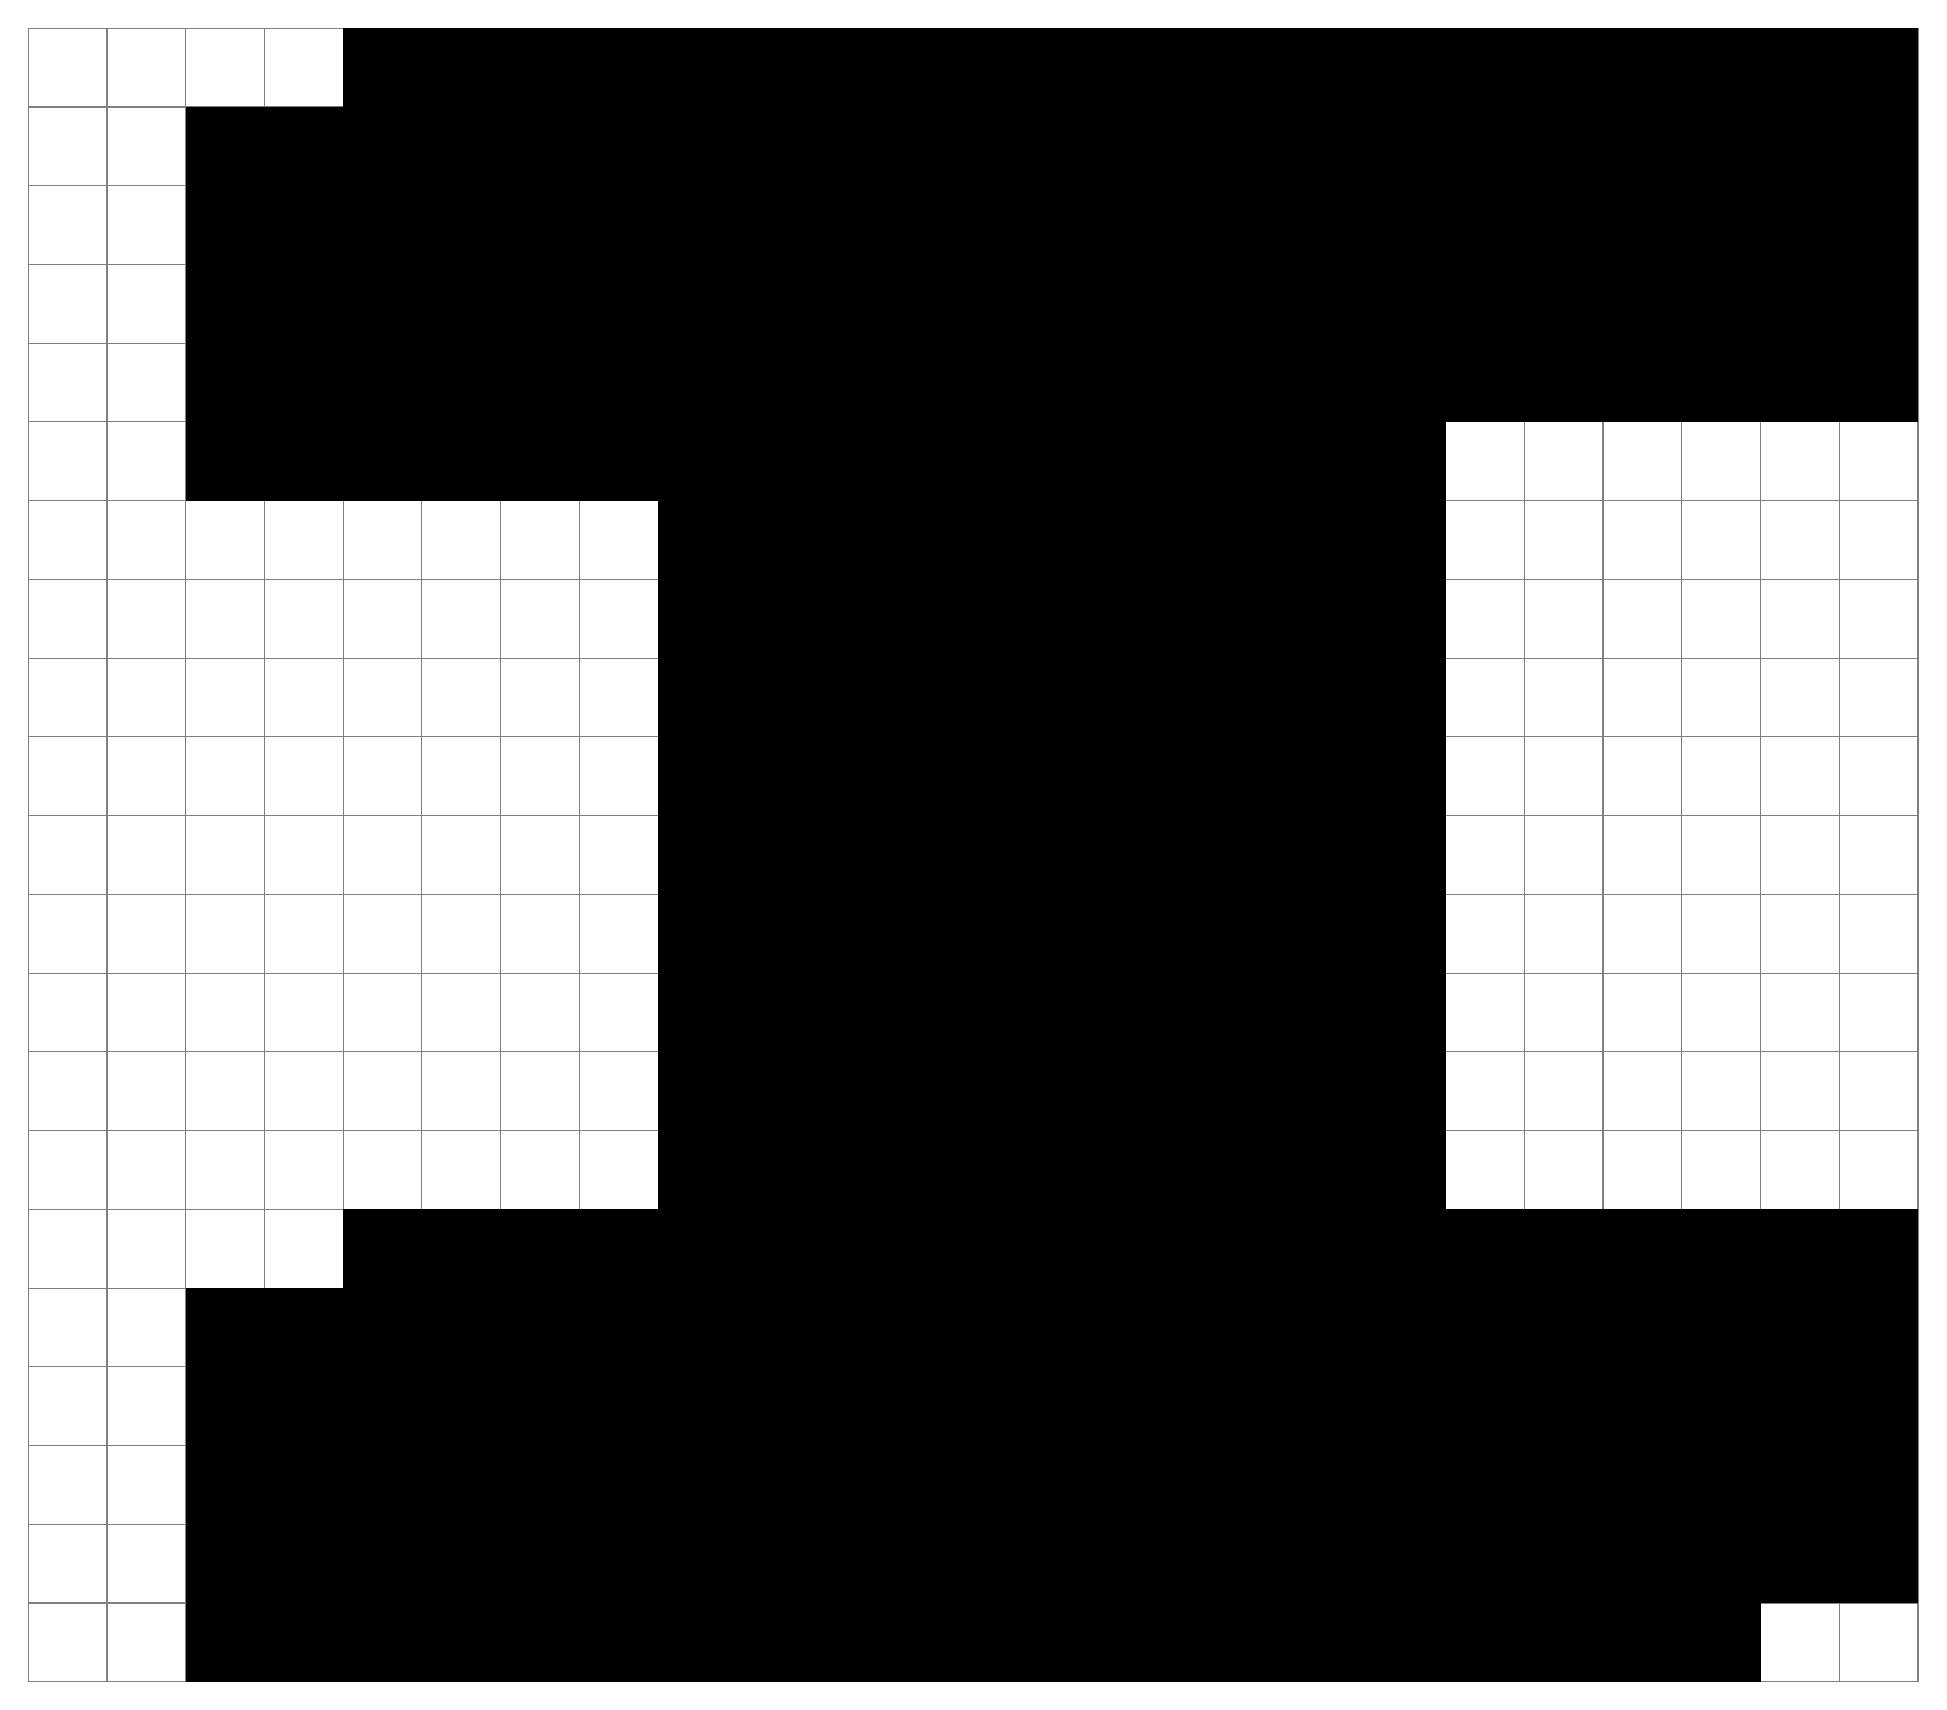
\begin{tikzpicture}

	\draw[step=1.0,gray,thin] (0,0) grid (24,21);
	\fill[\MULTICOLORTWO] (4,20) rectangle ++ (1,1);
	\fill[\MULTICOLORTWO] (5,20) rectangle ++ (1,1);
	\fill[\MULTICOLORTWO] (6,20) rectangle ++ (1,1);
	\fill[\MULTICOLORTWO] (7,20) rectangle ++ (1,1);
	\fill[\MULTICOLORTWO] (8,20) rectangle ++ (1,1);
	\fill[\MULTICOLORTWO] (9,20) rectangle ++ (1,1);
	\fill[\MULTICOLORTWO] (10,20) rectangle ++ (1,1);
	\fill[\MULTICOLORTWO] (11,20) rectangle ++ (1,1);
	\fill[\MULTICOLORTWO] (12,20) rectangle ++ (1,1);
	\fill[\MULTICOLORTWO] (13,20) rectangle ++ (1,1);
	\fill[\MULTICOLORTWO] (14,20) rectangle ++ (1,1);
	\fill[\MULTICOLORTWO] (15,20) rectangle ++ (1,1);
	\fill[\MULTICOLORTWO] (16,20) rectangle ++ (1,1);
	\fill[\MULTICOLORTWO] (17,20) rectangle ++ (1,1);
	\fill[\MULTICOLORTWO] (18,20) rectangle ++ (1,1);
	\fill[\MULTICOLORTWO] (19,20) rectangle ++ (1,1);
	\fill[\MULTICOLORTWO] (20,20) rectangle ++ (1,1);
	\fill[\MULTICOLORTWO] (21,20) rectangle ++ (1,1);
	\fill[\MULTICOLORTWO] (22,20) rectangle ++ (1,1);
	\fill[\MULTICOLORTWO] (23,20) rectangle ++ (1,1);
	\fill[\MULTICOLORONE] (2,19) rectangle ++ (1,1);
	\fill[\MULTICOLORONE] (3,19) rectangle ++ (1,1);
	\fill[\MULTICOLORTWO] (4,19) rectangle ++ (1,1);
	\fill[\MULTICOLORTWO] (5,19) rectangle ++ (1,1);
	\fill[\SPRITECOLOR] (6,19) rectangle ++ (1,1);
	\fill[\SPRITECOLOR] (7,19) rectangle ++ (1,1);
	\fill[\SPRITECOLOR] (8,19) rectangle ++ (1,1);
	\fill[\SPRITECOLOR] (9,19) rectangle ++ (1,1);
	\fill[\SPRITECOLOR] (10,19) rectangle ++ (1,1);
	\fill[\SPRITECOLOR] (11,19) rectangle ++ (1,1);
	\fill[\SPRITECOLOR] (12,19) rectangle ++ (1,1);
	\fill[\SPRITECOLOR] (13,19) rectangle ++ (1,1);
	\fill[\SPRITECOLOR] (14,19) rectangle ++ (1,1);
	\fill[\SPRITECOLOR] (15,19) rectangle ++ (1,1);
	\fill[\SPRITECOLOR] (16,19) rectangle ++ (1,1);
	\fill[\SPRITECOLOR] (17,19) rectangle ++ (1,1);
	\fill[\SPRITECOLOR] (18,19) rectangle ++ (1,1);
	\fill[\SPRITECOLOR] (19,19) rectangle ++ (1,1);
	\fill[\SPRITECOLOR] (20,19) rectangle ++ (1,1);
	\fill[\SPRITECOLOR] (21,19) rectangle ++ (1,1);
	\fill[\MULTICOLORTWO] (22,19) rectangle ++ (1,1);
	\fill[\MULTICOLORTWO] (23,19) rectangle ++ (1,1);
	\fill[\MULTICOLORONE] (2,18) rectangle ++ (1,1);
	\fill[\MULTICOLORONE] (3,18) rectangle ++ (1,1);
	\fill[\MULTICOLORTWO] (4,18) rectangle ++ (1,1);
	\fill[\MULTICOLORTWO] (5,18) rectangle ++ (1,1);
	\fill[\SPRITECOLOR] (6,18) rectangle ++ (1,1);
	\fill[\SPRITECOLOR] (7,18) rectangle ++ (1,1);
	\fill[\SPRITECOLOR] (8,18) rectangle ++ (1,1);
	\fill[\SPRITECOLOR] (9,18) rectangle ++ (1,1);
	\fill[\SPRITECOLOR] (10,18) rectangle ++ (1,1);
	\fill[\SPRITECOLOR] (11,18) rectangle ++ (1,1);
	\fill[\SPRITECOLOR] (12,18) rectangle ++ (1,1);
	\fill[\SPRITECOLOR] (13,18) rectangle ++ (1,1);
	\fill[\SPRITECOLOR] (14,18) rectangle ++ (1,1);
	\fill[\SPRITECOLOR] (15,18) rectangle ++ (1,1);
	\fill[\SPRITECOLOR] (16,18) rectangle ++ (1,1);
	\fill[\SPRITECOLOR] (17,18) rectangle ++ (1,1);
	\fill[\SPRITECOLOR] (18,18) rectangle ++ (1,1);
	\fill[\SPRITECOLOR] (19,18) rectangle ++ (1,1);
	\fill[\SPRITECOLOR] (20,18) rectangle ++ (1,1);
	\fill[\SPRITECOLOR] (21,18) rectangle ++ (1,1);
	\fill[\MULTICOLORTWO] (22,18) rectangle ++ (1,1);
	\fill[\MULTICOLORTWO] (23,18) rectangle ++ (1,1);
	\fill[\MULTICOLORONE] (2,17) rectangle ++ (1,1);
	\fill[\MULTICOLORONE] (3,17) rectangle ++ (1,1);
	\fill[\MULTICOLORTWO] (4,17) rectangle ++ (1,1);
	\fill[\MULTICOLORTWO] (5,17) rectangle ++ (1,1);
	\fill[\SPRITECOLOR] (6,17) rectangle ++ (1,1);
	\fill[\SPRITECOLOR] (7,17) rectangle ++ (1,1);
	\fill[\SPRITECOLOR] (8,17) rectangle ++ (1,1);
	\fill[\SPRITECOLOR] (9,17) rectangle ++ (1,1);
	\fill[\SPRITECOLOR] (10,17) rectangle ++ (1,1);
	\fill[\SPRITECOLOR] (11,17) rectangle ++ (1,1);
	\fill[\SPRITECOLOR] (12,17) rectangle ++ (1,1);
	\fill[\SPRITECOLOR] (13,17) rectangle ++ (1,1);
	\fill[\SPRITECOLOR] (14,17) rectangle ++ (1,1);
	\fill[\SPRITECOLOR] (15,17) rectangle ++ (1,1);
	\fill[\SPRITECOLOR] (16,17) rectangle ++ (1,1);
	\fill[\SPRITECOLOR] (17,17) rectangle ++ (1,1);
	\fill[\SPRITECOLOR] (18,17) rectangle ++ (1,1);
	\fill[\SPRITECOLOR] (19,17) rectangle ++ (1,1);
	\fill[\SPRITECOLOR] (20,17) rectangle ++ (1,1);
	\fill[\SPRITECOLOR] (21,17) rectangle ++ (1,1);
	\fill[\MULTICOLORTWO] (22,17) rectangle ++ (1,1);
	\fill[\MULTICOLORTWO] (23,17) rectangle ++ (1,1);
	\fill[\MULTICOLORONE] (2,16) rectangle ++ (1,1);
	\fill[\MULTICOLORONE] (3,16) rectangle ++ (1,1);
	\fill[\MULTICOLORTWO] (4,16) rectangle ++ (1,1);
	\fill[\MULTICOLORTWO] (5,16) rectangle ++ (1,1);
	\fill[\MULTICOLORTWO] (6,16) rectangle ++ (1,1);
	\fill[\MULTICOLORTWO] (7,16) rectangle ++ (1,1);
	\fill[\MULTICOLORTWO] (8,16) rectangle ++ (1,1);
	\fill[\MULTICOLORTWO] (9,16) rectangle ++ (1,1);
	\fill[\MULTICOLORTWO] (10,16) rectangle ++ (1,1);
	\fill[\MULTICOLORTWO] (11,16) rectangle ++ (1,1);
	\fill[\SPRITECOLOR] (12,16) rectangle ++ (1,1);
	\fill[\SPRITECOLOR] (13,16) rectangle ++ (1,1);
	\fill[\SPRITECOLOR] (14,16) rectangle ++ (1,1);
	\fill[\SPRITECOLOR] (15,16) rectangle ++ (1,1);
	\fill[\MULTICOLORTWO] (16,16) rectangle ++ (1,1);
	\fill[\MULTICOLORTWO] (17,16) rectangle ++ (1,1);
	\fill[\MULTICOLORTWO] (18,16) rectangle ++ (1,1);
	\fill[\MULTICOLORTWO] (19,16) rectangle ++ (1,1);
	\fill[\MULTICOLORTWO] (20,16) rectangle ++ (1,1);
	\fill[\MULTICOLORTWO] (21,16) rectangle ++ (1,1);
	\fill[\MULTICOLORTWO] (22,16) rectangle ++ (1,1);
	\fill[\MULTICOLORTWO] (23,16) rectangle ++ (1,1);
	\fill[\MULTICOLORONE] (2,15) rectangle ++ (1,1);
	\fill[\MULTICOLORONE] (3,15) rectangle ++ (1,1);
	\fill[\MULTICOLORONE] (4,15) rectangle ++ (1,1);
	\fill[\MULTICOLORONE] (5,15) rectangle ++ (1,1);
	\fill[\MULTICOLORONE] (6,15) rectangle ++ (1,1);
	\fill[\MULTICOLORONE] (7,15) rectangle ++ (1,1);
	\fill[\MULTICOLORONE] (8,15) rectangle ++ (1,1);
	\fill[\MULTICOLORONE] (9,15) rectangle ++ (1,1);
	\fill[\MULTICOLORTWO] (10,15) rectangle ++ (1,1);
	\fill[\MULTICOLORTWO] (11,15) rectangle ++ (1,1);
	\fill[\SPRITECOLOR] (12,15) rectangle ++ (1,1);
	\fill[\SPRITECOLOR] (13,15) rectangle ++ (1,1);
	\fill[\SPRITECOLOR] (14,15) rectangle ++ (1,1);
	\fill[\SPRITECOLOR] (15,15) rectangle ++ (1,1);
	\fill[\MULTICOLORTWO] (16,15) rectangle ++ (1,1);
	\fill[\MULTICOLORTWO] (17,15) rectangle ++ (1,1);
	\fill[\MULTICOLORONE] (8,14) rectangle ++ (1,1);
	\fill[\MULTICOLORONE] (9,14) rectangle ++ (1,1);
	\fill[\MULTICOLORTWO] (10,14) rectangle ++ (1,1);
	\fill[\MULTICOLORTWO] (11,14) rectangle ++ (1,1);
	\fill[\SPRITECOLOR] (12,14) rectangle ++ (1,1);
	\fill[\SPRITECOLOR] (13,14) rectangle ++ (1,1);
	\fill[\SPRITECOLOR] (14,14) rectangle ++ (1,1);
	\fill[\SPRITECOLOR] (15,14) rectangle ++ (1,1);
	\fill[\MULTICOLORTWO] (16,14) rectangle ++ (1,1);
	\fill[\MULTICOLORTWO] (17,14) rectangle ++ (1,1);
	\fill[\MULTICOLORONE] (8,13) rectangle ++ (1,1);
	\fill[\MULTICOLORONE] (9,13) rectangle ++ (1,1);
	\fill[\MULTICOLORTWO] (10,13) rectangle ++ (1,1);
	\fill[\MULTICOLORTWO] (11,13) rectangle ++ (1,1);
	\fill[\SPRITECOLOR] (12,13) rectangle ++ (1,1);
	\fill[\SPRITECOLOR] (13,13) rectangle ++ (1,1);
	\fill[\SPRITECOLOR] (14,13) rectangle ++ (1,1);
	\fill[\SPRITECOLOR] (15,13) rectangle ++ (1,1);
	\fill[\MULTICOLORTWO] (16,13) rectangle ++ (1,1);
	\fill[\MULTICOLORTWO] (17,13) rectangle ++ (1,1);
	\fill[\MULTICOLORONE] (8,12) rectangle ++ (1,1);
	\fill[\MULTICOLORONE] (9,12) rectangle ++ (1,1);
	\fill[\MULTICOLORTWO] (10,12) rectangle ++ (1,1);
	\fill[\MULTICOLORTWO] (11,12) rectangle ++ (1,1);
	\fill[\SPRITECOLOR] (12,12) rectangle ++ (1,1);
	\fill[\SPRITECOLOR] (13,12) rectangle ++ (1,1);
	\fill[\SPRITECOLOR] (14,12) rectangle ++ (1,1);
	\fill[\SPRITECOLOR] (15,12) rectangle ++ (1,1);
	\fill[\MULTICOLORTWO] (16,12) rectangle ++ (1,1);
	\fill[\MULTICOLORTWO] (17,12) rectangle ++ (1,1);
	\fill[\MULTICOLORONE] (8,11) rectangle ++ (1,1);
	\fill[\MULTICOLORONE] (9,11) rectangle ++ (1,1);
	\fill[\MULTICOLORTWO] (10,11) rectangle ++ (1,1);
	\fill[\MULTICOLORTWO] (11,11) rectangle ++ (1,1);
	\fill[\SPRITECOLOR] (12,11) rectangle ++ (1,1);
	\fill[\SPRITECOLOR] (13,11) rectangle ++ (1,1);
	\fill[\SPRITECOLOR] (14,11) rectangle ++ (1,1);
	\fill[\SPRITECOLOR] (15,11) rectangle ++ (1,1);
	\fill[\MULTICOLORTWO] (16,11) rectangle ++ (1,1);
	\fill[\MULTICOLORTWO] (17,11) rectangle ++ (1,1);
	\fill[\MULTICOLORONE] (8,10) rectangle ++ (1,1);
	\fill[\MULTICOLORONE] (9,10) rectangle ++ (1,1);
	\fill[\MULTICOLORTWO] (10,10) rectangle ++ (1,1);
	\fill[\MULTICOLORTWO] (11,10) rectangle ++ (1,1);
	\fill[\SPRITECOLOR] (12,10) rectangle ++ (1,1);
	\fill[\SPRITECOLOR] (13,10) rectangle ++ (1,1);
	\fill[\SPRITECOLOR] (14,10) rectangle ++ (1,1);
	\fill[\SPRITECOLOR] (15,10) rectangle ++ (1,1);
	\fill[\MULTICOLORTWO] (16,10) rectangle ++ (1,1);
	\fill[\MULTICOLORTWO] (17,10) rectangle ++ (1,1);
	\fill[\MULTICOLORONE] (8,9) rectangle ++ (1,1);
	\fill[\MULTICOLORONE] (9,9) rectangle ++ (1,1);
	\fill[\MULTICOLORTWO] (10,9) rectangle ++ (1,1);
	\fill[\MULTICOLORTWO] (11,9) rectangle ++ (1,1);
	\fill[\SPRITECOLOR] (12,9) rectangle ++ (1,1);
	\fill[\SPRITECOLOR] (13,9) rectangle ++ (1,1);
	\fill[\SPRITECOLOR] (14,9) rectangle ++ (1,1);
	\fill[\SPRITECOLOR] (15,9) rectangle ++ (1,1);
	\fill[\MULTICOLORTWO] (16,9) rectangle ++ (1,1);
	\fill[\MULTICOLORTWO] (17,9) rectangle ++ (1,1);
	\fill[\MULTICOLORONE] (8,8) rectangle ++ (1,1);
	\fill[\MULTICOLORONE] (9,8) rectangle ++ (1,1);
	\fill[\MULTICOLORTWO] (10,8) rectangle ++ (1,1);
	\fill[\MULTICOLORTWO] (11,8) rectangle ++ (1,1);
	\fill[\SPRITECOLOR] (12,8) rectangle ++ (1,1);
	\fill[\SPRITECOLOR] (13,8) rectangle ++ (1,1);
	\fill[\SPRITECOLOR] (14,8) rectangle ++ (1,1);
	\fill[\SPRITECOLOR] (15,8) rectangle ++ (1,1);
	\fill[\MULTICOLORTWO] (16,8) rectangle ++ (1,1);
	\fill[\MULTICOLORTWO] (17,8) rectangle ++ (1,1);
	\fill[\MULTICOLORONE] (8,7) rectangle ++ (1,1);
	\fill[\MULTICOLORONE] (9,7) rectangle ++ (1,1);
	\fill[\MULTICOLORTWO] (10,7) rectangle ++ (1,1);
	\fill[\MULTICOLORTWO] (11,7) rectangle ++ (1,1);
	\fill[\SPRITECOLOR] (12,7) rectangle ++ (1,1);
	\fill[\SPRITECOLOR] (13,7) rectangle ++ (1,1);
	\fill[\SPRITECOLOR] (14,7) rectangle ++ (1,1);
	\fill[\SPRITECOLOR] (15,7) rectangle ++ (1,1);
	\fill[\MULTICOLORTWO] (16,7) rectangle ++ (1,1);
	\fill[\MULTICOLORTWO] (17,7) rectangle ++ (1,1);
	\fill[\MULTICOLORONE] (8,6) rectangle ++ (1,1);
	\fill[\MULTICOLORONE] (9,6) rectangle ++ (1,1);
	\fill[\MULTICOLORTWO] (10,6) rectangle ++ (1,1);
	\fill[\MULTICOLORTWO] (11,6) rectangle ++ (1,1);
	\fill[\SPRITECOLOR] (12,6) rectangle ++ (1,1);
	\fill[\SPRITECOLOR] (13,6) rectangle ++ (1,1);
	\fill[\SPRITECOLOR] (14,6) rectangle ++ (1,1);
	\fill[\SPRITECOLOR] (15,6) rectangle ++ (1,1);
	\fill[\MULTICOLORTWO] (16,6) rectangle ++ (1,1);
	\fill[\MULTICOLORTWO] (17,6) rectangle ++ (1,1);
	\fill[\MULTICOLORTWO] (4,5) rectangle ++ (1,1);
	\fill[\MULTICOLORTWO] (5,5) rectangle ++ (1,1);
	\fill[\MULTICOLORTWO] (6,5) rectangle ++ (1,1);
	\fill[\MULTICOLORTWO] (7,5) rectangle ++ (1,1);
	\fill[\MULTICOLORTWO] (8,5) rectangle ++ (1,1);
	\fill[\MULTICOLORTWO] (9,5) rectangle ++ (1,1);
	\fill[\MULTICOLORTWO] (10,5) rectangle ++ (1,1);
	\fill[\MULTICOLORTWO] (11,5) rectangle ++ (1,1);
	\fill[\SPRITECOLOR] (12,5) rectangle ++ (1,1);
	\fill[\SPRITECOLOR] (13,5) rectangle ++ (1,1);
	\fill[\SPRITECOLOR] (14,5) rectangle ++ (1,1);
	\fill[\SPRITECOLOR] (15,5) rectangle ++ (1,1);
	\fill[\MULTICOLORTWO] (16,5) rectangle ++ (1,1);
	\fill[\MULTICOLORTWO] (17,5) rectangle ++ (1,1);
	\fill[\MULTICOLORTWO] (18,5) rectangle ++ (1,1);
	\fill[\MULTICOLORTWO] (19,5) rectangle ++ (1,1);
	\fill[\MULTICOLORTWO] (20,5) rectangle ++ (1,1);
	\fill[\MULTICOLORTWO] (21,5) rectangle ++ (1,1);
	\fill[\MULTICOLORTWO] (22,5) rectangle ++ (1,1);
	\fill[\MULTICOLORTWO] (23,5) rectangle ++ (1,1);
	\fill[\MULTICOLORONE] (2,4) rectangle ++ (1,1);
	\fill[\MULTICOLORONE] (3,4) rectangle ++ (1,1);
	\fill[\MULTICOLORTWO] (4,4) rectangle ++ (1,1);
	\fill[\MULTICOLORTWO] (5,4) rectangle ++ (1,1);
	\fill[\SPRITECOLOR] (6,4) rectangle ++ (1,1);
	\fill[\SPRITECOLOR] (7,4) rectangle ++ (1,1);
	\fill[\SPRITECOLOR] (8,4) rectangle ++ (1,1);
	\fill[\SPRITECOLOR] (9,4) rectangle ++ (1,1);
	\fill[\SPRITECOLOR] (10,4) rectangle ++ (1,1);
	\fill[\SPRITECOLOR] (11,4) rectangle ++ (1,1);
	\fill[\SPRITECOLOR] (12,4) rectangle ++ (1,1);
	\fill[\SPRITECOLOR] (13,4) rectangle ++ (1,1);
	\fill[\SPRITECOLOR] (14,4) rectangle ++ (1,1);
	\fill[\SPRITECOLOR] (15,4) rectangle ++ (1,1);
	\fill[\SPRITECOLOR] (16,4) rectangle ++ (1,1);
	\fill[\SPRITECOLOR] (17,4) rectangle ++ (1,1);
	\fill[\SPRITECOLOR] (18,4) rectangle ++ (1,1);
	\fill[\SPRITECOLOR] (19,4) rectangle ++ (1,1);
	\fill[\SPRITECOLOR] (20,4) rectangle ++ (1,1);
	\fill[\SPRITECOLOR] (21,4) rectangle ++ (1,1);
	\fill[\MULTICOLORTWO] (22,4) rectangle ++ (1,1);
	\fill[\MULTICOLORTWO] (23,4) rectangle ++ (1,1);
	\fill[\MULTICOLORONE] (2,3) rectangle ++ (1,1);
	\fill[\MULTICOLORONE] (3,3) rectangle ++ (1,1);
	\fill[\MULTICOLORTWO] (4,3) rectangle ++ (1,1);
	\fill[\MULTICOLORTWO] (5,3) rectangle ++ (1,1);
	\fill[\SPRITECOLOR] (6,3) rectangle ++ (1,1);
	\fill[\SPRITECOLOR] (7,3) rectangle ++ (1,1);
	\fill[\SPRITECOLOR] (8,3) rectangle ++ (1,1);
	\fill[\SPRITECOLOR] (9,3) rectangle ++ (1,1);
	\fill[\SPRITECOLOR] (10,3) rectangle ++ (1,1);
	\fill[\SPRITECOLOR] (11,3) rectangle ++ (1,1);
	\fill[\SPRITECOLOR] (12,3) rectangle ++ (1,1);
	\fill[\SPRITECOLOR] (13,3) rectangle ++ (1,1);
	\fill[\SPRITECOLOR] (14,3) rectangle ++ (1,1);
	\fill[\SPRITECOLOR] (15,3) rectangle ++ (1,1);
	\fill[\SPRITECOLOR] (16,3) rectangle ++ (1,1);
	\fill[\SPRITECOLOR] (17,3) rectangle ++ (1,1);
	\fill[\SPRITECOLOR] (18,3) rectangle ++ (1,1);
	\fill[\SPRITECOLOR] (19,3) rectangle ++ (1,1);
	\fill[\SPRITECOLOR] (20,3) rectangle ++ (1,1);
	\fill[\SPRITECOLOR] (21,3) rectangle ++ (1,1);
	\fill[\MULTICOLORTWO] (22,3) rectangle ++ (1,1);
	\fill[\MULTICOLORTWO] (23,3) rectangle ++ (1,1);
	\fill[\MULTICOLORONE] (2,2) rectangle ++ (1,1);
	\fill[\MULTICOLORONE] (3,2) rectangle ++ (1,1);
	\fill[\MULTICOLORTWO] (4,2) rectangle ++ (1,1);
	\fill[\MULTICOLORTWO] (5,2) rectangle ++ (1,1);
	\fill[\SPRITECOLOR] (6,2) rectangle ++ (1,1);
	\fill[\SPRITECOLOR] (7,2) rectangle ++ (1,1);
	\fill[\SPRITECOLOR] (8,2) rectangle ++ (1,1);
	\fill[\SPRITECOLOR] (9,2) rectangle ++ (1,1);
	\fill[\SPRITECOLOR] (10,2) rectangle ++ (1,1);
	\fill[\SPRITECOLOR] (11,2) rectangle ++ (1,1);
	\fill[\SPRITECOLOR] (12,2) rectangle ++ (1,1);
	\fill[\SPRITECOLOR] (13,2) rectangle ++ (1,1);
	\fill[\SPRITECOLOR] (14,2) rectangle ++ (1,1);
	\fill[\SPRITECOLOR] (15,2) rectangle ++ (1,1);
	\fill[\SPRITECOLOR] (16,2) rectangle ++ (1,1);
	\fill[\SPRITECOLOR] (17,2) rectangle ++ (1,1);
	\fill[\SPRITECOLOR] (18,2) rectangle ++ (1,1);
	\fill[\SPRITECOLOR] (19,2) rectangle ++ (1,1);
	\fill[\SPRITECOLOR] (20,2) rectangle ++ (1,1);
	\fill[\SPRITECOLOR] (21,2) rectangle ++ (1,1);
	\fill[\MULTICOLORTWO] (22,2) rectangle ++ (1,1);
	\fill[\MULTICOLORTWO] (23,2) rectangle ++ (1,1);
	\fill[\MULTICOLORONE] (2,1) rectangle ++ (1,1);
	\fill[\MULTICOLORONE] (3,1) rectangle ++ (1,1);
	\fill[\MULTICOLORTWO] (4,1) rectangle ++ (1,1);
	\fill[\MULTICOLORTWO] (5,1) rectangle ++ (1,1);
	\fill[\MULTICOLORTWO] (6,1) rectangle ++ (1,1);
	\fill[\MULTICOLORTWO] (7,1) rectangle ++ (1,1);
	\fill[\MULTICOLORTWO] (8,1) rectangle ++ (1,1);
	\fill[\MULTICOLORTWO] (9,1) rectangle ++ (1,1);
	\fill[\MULTICOLORTWO] (10,1) rectangle ++ (1,1);
	\fill[\MULTICOLORTWO] (11,1) rectangle ++ (1,1);
	\fill[\MULTICOLORTWO] (12,1) rectangle ++ (1,1);
	\fill[\MULTICOLORTWO] (13,1) rectangle ++ (1,1);
	\fill[\MULTICOLORTWO] (14,1) rectangle ++ (1,1);
	\fill[\MULTICOLORTWO] (15,1) rectangle ++ (1,1);
	\fill[\MULTICOLORTWO] (16,1) rectangle ++ (1,1);
	\fill[\MULTICOLORTWO] (17,1) rectangle ++ (1,1);
	\fill[\MULTICOLORTWO] (18,1) rectangle ++ (1,1);
	\fill[\MULTICOLORTWO] (19,1) rectangle ++ (1,1);
	\fill[\MULTICOLORTWO] (20,1) rectangle ++ (1,1);
	\fill[\MULTICOLORTWO] (21,1) rectangle ++ (1,1);
	\fill[\MULTICOLORTWO] (22,1) rectangle ++ (1,1);
	\fill[\MULTICOLORTWO] (23,1) rectangle ++ (1,1);
	\fill[\MULTICOLORONE] (2,0) rectangle ++ (1,1);
	\fill[\MULTICOLORONE] (3,0) rectangle ++ (1,1);
	\fill[\MULTICOLORONE] (4,0) rectangle ++ (1,1);
	\fill[\MULTICOLORONE] (5,0) rectangle ++ (1,1);
	\fill[\MULTICOLORONE] (6,0) rectangle ++ (1,1);
	\fill[\MULTICOLORONE] (7,0) rectangle ++ (1,1);
	\fill[\MULTICOLORONE] (8,0) rectangle ++ (1,1);
	\fill[\MULTICOLORONE] (9,0) rectangle ++ (1,1);
	\fill[\MULTICOLORONE] (10,0) rectangle ++ (1,1);
	\fill[\MULTICOLORONE] (11,0) rectangle ++ (1,1);
	\fill[\MULTICOLORONE] (12,0) rectangle ++ (1,1);
	\fill[\MULTICOLORONE] (13,0) rectangle ++ (1,1);
	\fill[\MULTICOLORONE] (14,0) rectangle ++ (1,1);
	\fill[\MULTICOLORONE] (15,0) rectangle ++ (1,1);
	\fill[\MULTICOLORONE] (16,0) rectangle ++ (1,1);
	\fill[\MULTICOLORONE] (17,0) rectangle ++ (1,1);
	\fill[\MULTICOLORONE] (18,0) rectangle ++ (1,1);
	\fill[\MULTICOLORONE] (19,0) rectangle ++ (1,1);
	\fill[\MULTICOLORONE] (20,0) rectangle ++ (1,1);
	\fill[\MULTICOLORONE] (21,0) rectangle ++ (1,1);

      \end{tikzpicture}
    \end{adjustbox}
  }\caption{BIG\_I}
\end{figure}

	\end{subfigure}
} &
\makecell[l]{
	\begin{subfigure}{0.3\textwidth}
    \def\MULTICOLORONE{gray}
    \def\MULTICOLORTWO{black}
    \def\SPRITECOLOR{green}
		
\begin{figure}[H]
  {
    \setlength{\tabcolsep}{3.0pt}
    \setlength\cmidrulewidth{\heavyrulewidth} % Make cmidrule = 
    \begin{adjustbox}{width=3cm,center}
      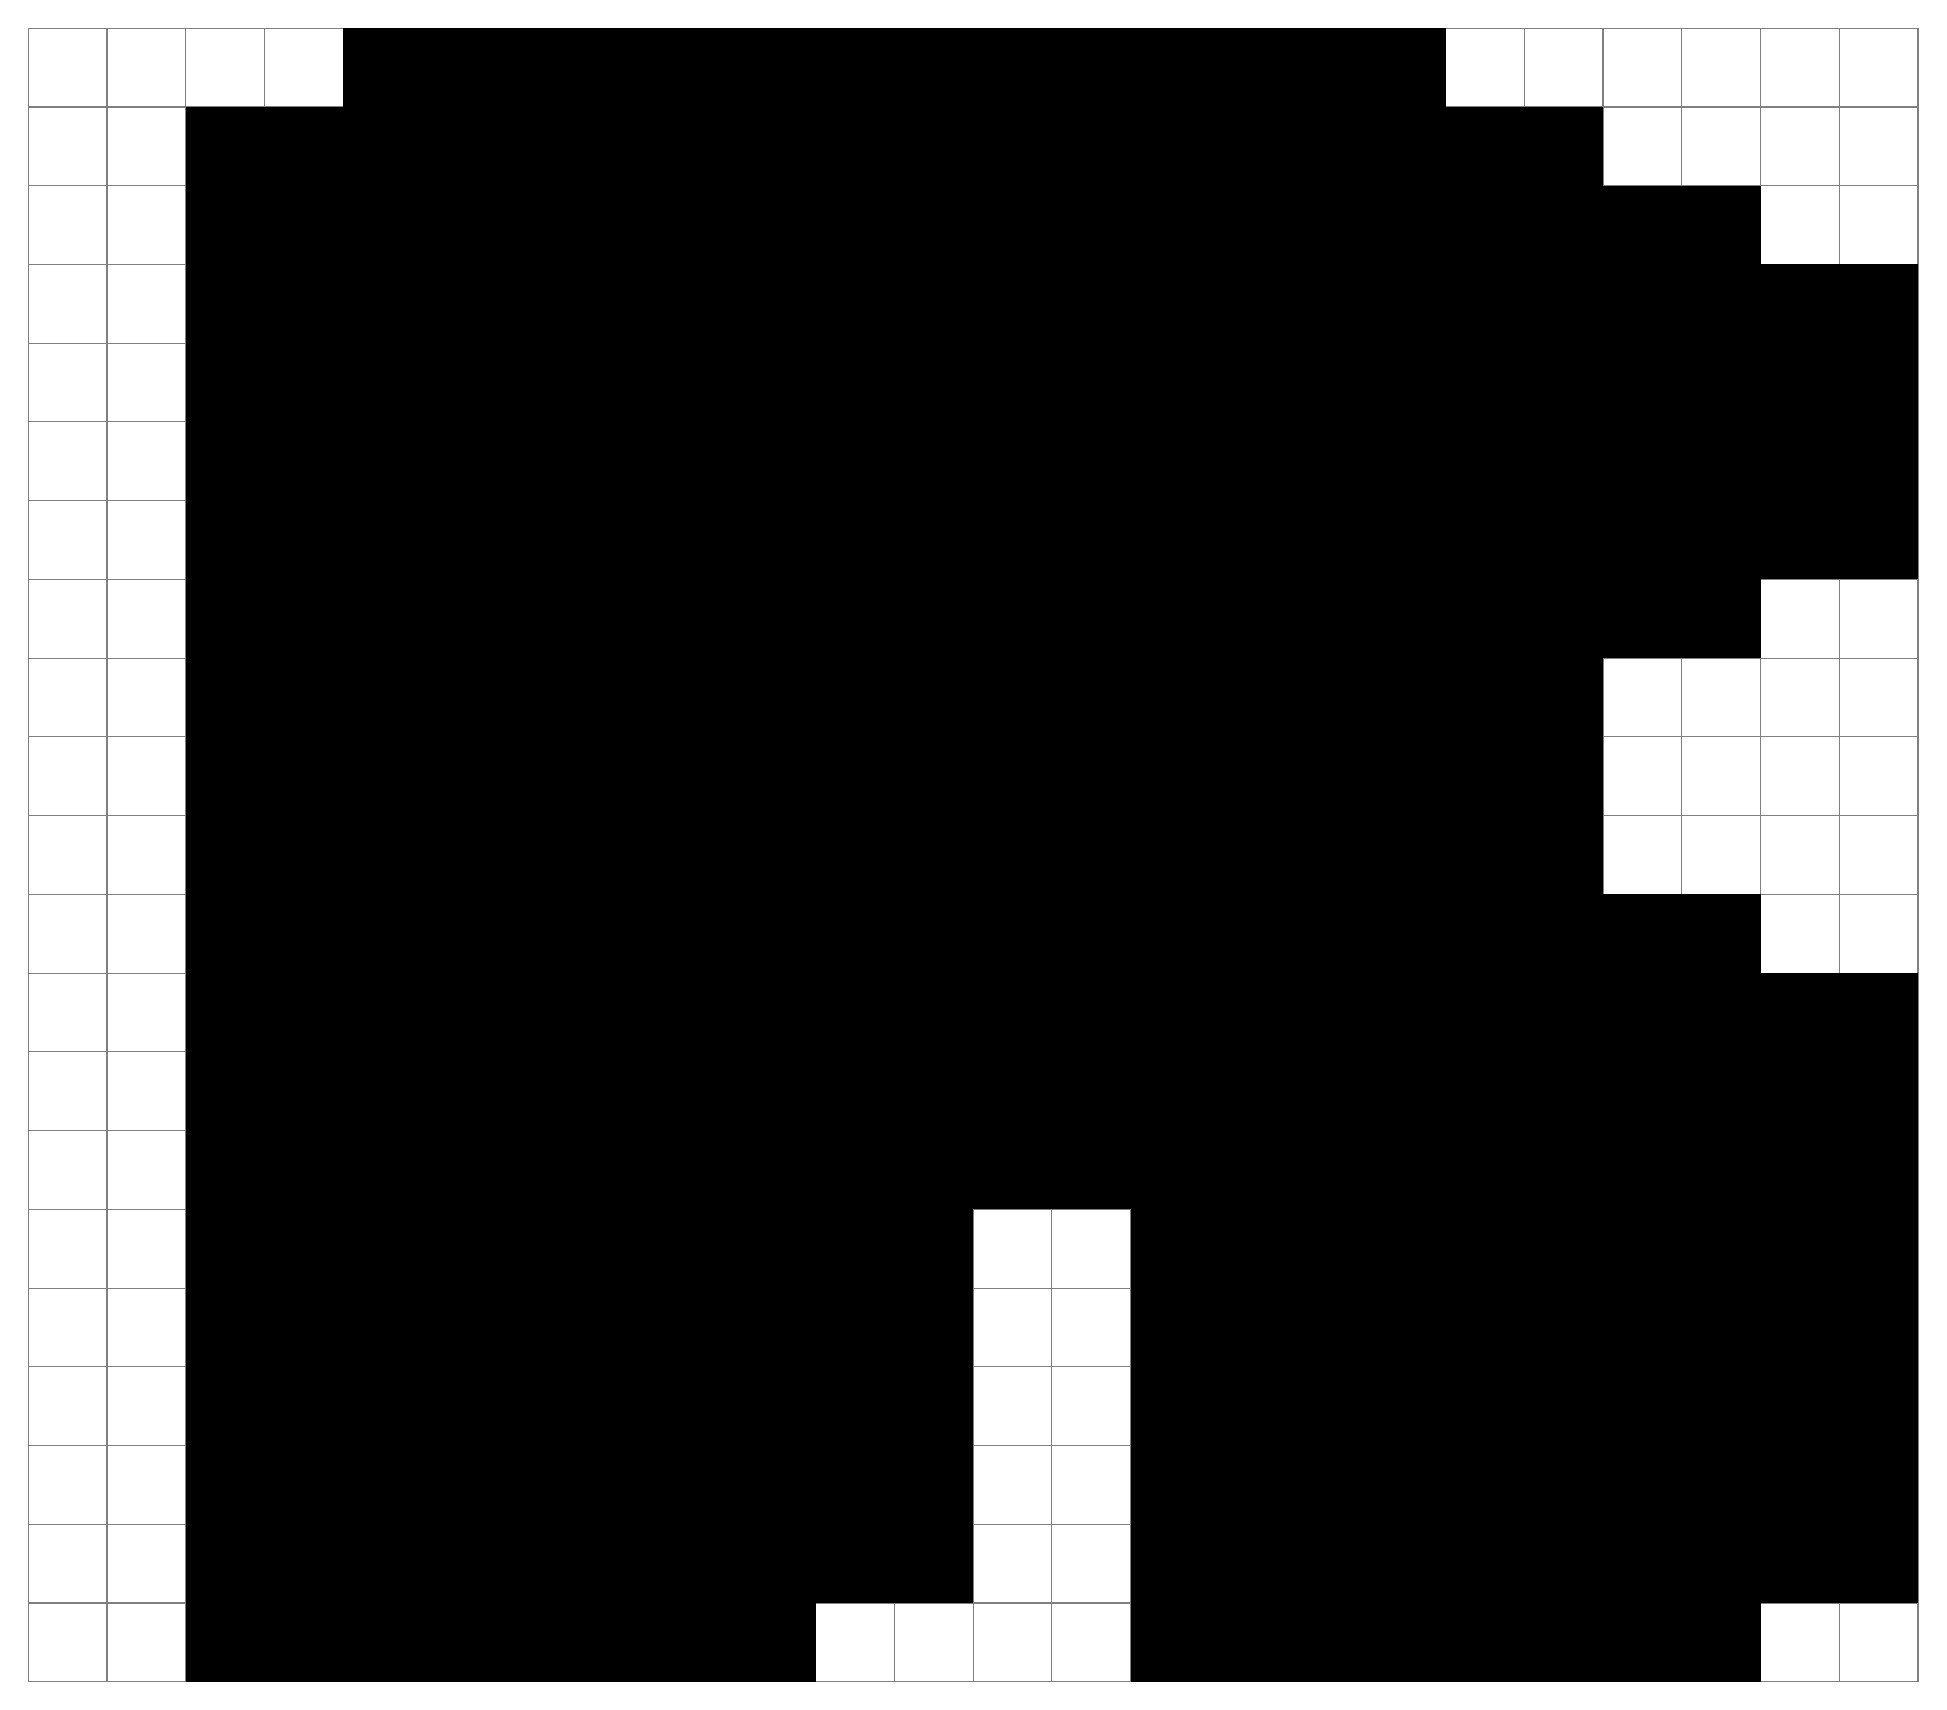
\begin{tikzpicture}

	\draw[step=1.0,gray,thin] (0,0) grid (24,21);
	\fill[\MULTICOLORTWO] (4,20) rectangle ++ (1,1);
	\fill[\MULTICOLORTWO] (5,20) rectangle ++ (1,1);
	\fill[\MULTICOLORTWO] (6,20) rectangle ++ (1,1);
	\fill[\MULTICOLORTWO] (7,20) rectangle ++ (1,1);
	\fill[\MULTICOLORTWO] (8,20) rectangle ++ (1,1);
	\fill[\MULTICOLORTWO] (9,20) rectangle ++ (1,1);
	\fill[\MULTICOLORTWO] (10,20) rectangle ++ (1,1);
	\fill[\MULTICOLORTWO] (11,20) rectangle ++ (1,1);
	\fill[\MULTICOLORTWO] (12,20) rectangle ++ (1,1);
	\fill[\MULTICOLORTWO] (13,20) rectangle ++ (1,1);
	\fill[\MULTICOLORTWO] (14,20) rectangle ++ (1,1);
	\fill[\MULTICOLORTWO] (15,20) rectangle ++ (1,1);
	\fill[\MULTICOLORTWO] (16,20) rectangle ++ (1,1);
	\fill[\MULTICOLORTWO] (17,20) rectangle ++ (1,1);
	\fill[\MULTICOLORONE] (2,19) rectangle ++ (1,1);
	\fill[\MULTICOLORONE] (3,19) rectangle ++ (1,1);
	\fill[\MULTICOLORTWO] (4,19) rectangle ++ (1,1);
	\fill[\MULTICOLORTWO] (5,19) rectangle ++ (1,1);
	\fill[\SPRITECOLOR] (6,19) rectangle ++ (1,1);
	\fill[\SPRITECOLOR] (7,19) rectangle ++ (1,1);
	\fill[\SPRITECOLOR] (8,19) rectangle ++ (1,1);
	\fill[\SPRITECOLOR] (9,19) rectangle ++ (1,1);
	\fill[\SPRITECOLOR] (10,19) rectangle ++ (1,1);
	\fill[\SPRITECOLOR] (11,19) rectangle ++ (1,1);
	\fill[\SPRITECOLOR] (12,19) rectangle ++ (1,1);
	\fill[\SPRITECOLOR] (13,19) rectangle ++ (1,1);
	\fill[\SPRITECOLOR] (14,19) rectangle ++ (1,1);
	\fill[\SPRITECOLOR] (15,19) rectangle ++ (1,1);
	\fill[\SPRITECOLOR] (16,19) rectangle ++ (1,1);
	\fill[\SPRITECOLOR] (17,19) rectangle ++ (1,1);
	\fill[\MULTICOLORTWO] (18,19) rectangle ++ (1,1);
	\fill[\MULTICOLORTWO] (19,19) rectangle ++ (1,1);
	\fill[\MULTICOLORONE] (2,18) rectangle ++ (1,1);
	\fill[\MULTICOLORONE] (3,18) rectangle ++ (1,1);
	\fill[\MULTICOLORTWO] (4,18) rectangle ++ (1,1);
	\fill[\MULTICOLORTWO] (5,18) rectangle ++ (1,1);
	\fill[\SPRITECOLOR] (6,18) rectangle ++ (1,1);
	\fill[\SPRITECOLOR] (7,18) rectangle ++ (1,1);
	\fill[\SPRITECOLOR] (8,18) rectangle ++ (1,1);
	\fill[\SPRITECOLOR] (9,18) rectangle ++ (1,1);
	\fill[\SPRITECOLOR] (10,18) rectangle ++ (1,1);
	\fill[\SPRITECOLOR] (11,18) rectangle ++ (1,1);
	\fill[\SPRITECOLOR] (12,18) rectangle ++ (1,1);
	\fill[\SPRITECOLOR] (13,18) rectangle ++ (1,1);
	\fill[\SPRITECOLOR] (14,18) rectangle ++ (1,1);
	\fill[\SPRITECOLOR] (15,18) rectangle ++ (1,1);
	\fill[\SPRITECOLOR] (16,18) rectangle ++ (1,1);
	\fill[\SPRITECOLOR] (17,18) rectangle ++ (1,1);
	\fill[\SPRITECOLOR] (18,18) rectangle ++ (1,1);
	\fill[\SPRITECOLOR] (19,18) rectangle ++ (1,1);
	\fill[\MULTICOLORTWO] (20,18) rectangle ++ (1,1);
	\fill[\MULTICOLORTWO] (21,18) rectangle ++ (1,1);
	\fill[\MULTICOLORONE] (2,17) rectangle ++ (1,1);
	\fill[\MULTICOLORONE] (3,17) rectangle ++ (1,1);
	\fill[\MULTICOLORTWO] (4,17) rectangle ++ (1,1);
	\fill[\MULTICOLORTWO] (5,17) rectangle ++ (1,1);
	\fill[\SPRITECOLOR] (6,17) rectangle ++ (1,1);
	\fill[\SPRITECOLOR] (7,17) rectangle ++ (1,1);
	\fill[\SPRITECOLOR] (8,17) rectangle ++ (1,1);
	\fill[\SPRITECOLOR] (9,17) rectangle ++ (1,1);
	\fill[\SPRITECOLOR] (10,17) rectangle ++ (1,1);
	\fill[\SPRITECOLOR] (11,17) rectangle ++ (1,1);
	\fill[\SPRITECOLOR] (12,17) rectangle ++ (1,1);
	\fill[\SPRITECOLOR] (13,17) rectangle ++ (1,1);
	\fill[\SPRITECOLOR] (14,17) rectangle ++ (1,1);
	\fill[\SPRITECOLOR] (15,17) rectangle ++ (1,1);
	\fill[\SPRITECOLOR] (16,17) rectangle ++ (1,1);
	\fill[\SPRITECOLOR] (17,17) rectangle ++ (1,1);
	\fill[\SPRITECOLOR] (18,17) rectangle ++ (1,1);
	\fill[\SPRITECOLOR] (19,17) rectangle ++ (1,1);
	\fill[\SPRITECOLOR] (20,17) rectangle ++ (1,1);
	\fill[\SPRITECOLOR] (21,17) rectangle ++ (1,1);
	\fill[\MULTICOLORTWO] (22,17) rectangle ++ (1,1);
	\fill[\MULTICOLORTWO] (23,17) rectangle ++ (1,1);
	\fill[\MULTICOLORONE] (2,16) rectangle ++ (1,1);
	\fill[\MULTICOLORONE] (3,16) rectangle ++ (1,1);
	\fill[\MULTICOLORTWO] (4,16) rectangle ++ (1,1);
	\fill[\MULTICOLORTWO] (5,16) rectangle ++ (1,1);
	\fill[\SPRITECOLOR] (6,16) rectangle ++ (1,1);
	\fill[\SPRITECOLOR] (7,16) rectangle ++ (1,1);
	\fill[\SPRITECOLOR] (8,16) rectangle ++ (1,1);
	\fill[\SPRITECOLOR] (9,16) rectangle ++ (1,1);
	\fill[\MULTICOLORTWO] (10,16) rectangle ++ (1,1);
	\fill[\MULTICOLORTWO] (11,16) rectangle ++ (1,1);
	\fill[\MULTICOLORTWO] (12,16) rectangle ++ (1,1);
	\fill[\MULTICOLORTWO] (13,16) rectangle ++ (1,1);
	\fill[\SPRITECOLOR] (14,16) rectangle ++ (1,1);
	\fill[\SPRITECOLOR] (15,16) rectangle ++ (1,1);
	\fill[\SPRITECOLOR] (16,16) rectangle ++ (1,1);
	\fill[\SPRITECOLOR] (17,16) rectangle ++ (1,1);
	\fill[\SPRITECOLOR] (18,16) rectangle ++ (1,1);
	\fill[\SPRITECOLOR] (19,16) rectangle ++ (1,1);
	\fill[\SPRITECOLOR] (20,16) rectangle ++ (1,1);
	\fill[\SPRITECOLOR] (21,16) rectangle ++ (1,1);
	\fill[\MULTICOLORTWO] (22,16) rectangle ++ (1,1);
	\fill[\MULTICOLORTWO] (23,16) rectangle ++ (1,1);
	\fill[\MULTICOLORONE] (2,15) rectangle ++ (1,1);
	\fill[\MULTICOLORONE] (3,15) rectangle ++ (1,1);
	\fill[\MULTICOLORTWO] (4,15) rectangle ++ (1,1);
	\fill[\MULTICOLORTWO] (5,15) rectangle ++ (1,1);
	\fill[\SPRITECOLOR] (6,15) rectangle ++ (1,1);
	\fill[\SPRITECOLOR] (7,15) rectangle ++ (1,1);
	\fill[\SPRITECOLOR] (8,15) rectangle ++ (1,1);
	\fill[\SPRITECOLOR] (9,15) rectangle ++ (1,1);
	\fill[\MULTICOLORTWO] (10,15) rectangle ++ (1,1);
	\fill[\MULTICOLORTWO] (11,15) rectangle ++ (1,1);
	\fill[\MULTICOLORONE] (12,15) rectangle ++ (1,1);
	\fill[\MULTICOLORONE] (13,15) rectangle ++ (1,1);
	\fill[\MULTICOLORTWO] (14,15) rectangle ++ (1,1);
	\fill[\MULTICOLORTWO] (15,15) rectangle ++ (1,1);
	\fill[\SPRITECOLOR] (16,15) rectangle ++ (1,1);
	\fill[\SPRITECOLOR] (17,15) rectangle ++ (1,1);
	\fill[\SPRITECOLOR] (18,15) rectangle ++ (1,1);
	\fill[\SPRITECOLOR] (19,15) rectangle ++ (1,1);
	\fill[\SPRITECOLOR] (20,15) rectangle ++ (1,1);
	\fill[\SPRITECOLOR] (21,15) rectangle ++ (1,1);
	\fill[\MULTICOLORTWO] (22,15) rectangle ++ (1,1);
	\fill[\MULTICOLORTWO] (23,15) rectangle ++ (1,1);
	\fill[\MULTICOLORONE] (2,14) rectangle ++ (1,1);
	\fill[\MULTICOLORONE] (3,14) rectangle ++ (1,1);
	\fill[\MULTICOLORTWO] (4,14) rectangle ++ (1,1);
	\fill[\MULTICOLORTWO] (5,14) rectangle ++ (1,1);
	\fill[\SPRITECOLOR] (6,14) rectangle ++ (1,1);
	\fill[\SPRITECOLOR] (7,14) rectangle ++ (1,1);
	\fill[\SPRITECOLOR] (8,14) rectangle ++ (1,1);
	\fill[\SPRITECOLOR] (9,14) rectangle ++ (1,1);
	\fill[\MULTICOLORTWO] (10,14) rectangle ++ (1,1);
	\fill[\MULTICOLORTWO] (11,14) rectangle ++ (1,1);
	\fill[\MULTICOLORONE] (12,14) rectangle ++ (1,1);
	\fill[\MULTICOLORONE] (13,14) rectangle ++ (1,1);
	\fill[\MULTICOLORTWO] (14,14) rectangle ++ (1,1);
	\fill[\MULTICOLORTWO] (15,14) rectangle ++ (1,1);
	\fill[\SPRITECOLOR] (16,14) rectangle ++ (1,1);
	\fill[\SPRITECOLOR] (17,14) rectangle ++ (1,1);
	\fill[\SPRITECOLOR] (18,14) rectangle ++ (1,1);
	\fill[\SPRITECOLOR] (19,14) rectangle ++ (1,1);
	\fill[\SPRITECOLOR] (20,14) rectangle ++ (1,1);
	\fill[\SPRITECOLOR] (21,14) rectangle ++ (1,1);
	\fill[\MULTICOLORTWO] (22,14) rectangle ++ (1,1);
	\fill[\MULTICOLORTWO] (23,14) rectangle ++ (1,1);
	\fill[\MULTICOLORONE] (2,13) rectangle ++ (1,1);
	\fill[\MULTICOLORONE] (3,13) rectangle ++ (1,1);
	\fill[\MULTICOLORTWO] (4,13) rectangle ++ (1,1);
	\fill[\MULTICOLORTWO] (5,13) rectangle ++ (1,1);
	\fill[\SPRITECOLOR] (6,13) rectangle ++ (1,1);
	\fill[\SPRITECOLOR] (7,13) rectangle ++ (1,1);
	\fill[\SPRITECOLOR] (8,13) rectangle ++ (1,1);
	\fill[\SPRITECOLOR] (9,13) rectangle ++ (1,1);
	\fill[\MULTICOLORTWO] (10,13) rectangle ++ (1,1);
	\fill[\MULTICOLORTWO] (11,13) rectangle ++ (1,1);
	\fill[\MULTICOLORONE] (12,13) rectangle ++ (1,1);
	\fill[\MULTICOLORONE] (13,13) rectangle ++ (1,1);
	\fill[\MULTICOLORTWO] (14,13) rectangle ++ (1,1);
	\fill[\MULTICOLORTWO] (15,13) rectangle ++ (1,1);
	\fill[\SPRITECOLOR] (16,13) rectangle ++ (1,1);
	\fill[\SPRITECOLOR] (17,13) rectangle ++ (1,1);
	\fill[\SPRITECOLOR] (18,13) rectangle ++ (1,1);
	\fill[\SPRITECOLOR] (19,13) rectangle ++ (1,1);
	\fill[\MULTICOLORTWO] (20,13) rectangle ++ (1,1);
	\fill[\MULTICOLORTWO] (21,13) rectangle ++ (1,1);
	\fill[\MULTICOLORONE] (2,12) rectangle ++ (1,1);
	\fill[\MULTICOLORONE] (3,12) rectangle ++ (1,1);
	\fill[\MULTICOLORTWO] (4,12) rectangle ++ (1,1);
	\fill[\MULTICOLORTWO] (5,12) rectangle ++ (1,1);
	\fill[\SPRITECOLOR] (6,12) rectangle ++ (1,1);
	\fill[\SPRITECOLOR] (7,12) rectangle ++ (1,1);
	\fill[\SPRITECOLOR] (8,12) rectangle ++ (1,1);
	\fill[\SPRITECOLOR] (9,12) rectangle ++ (1,1);
	\fill[\MULTICOLORTWO] (10,12) rectangle ++ (1,1);
	\fill[\MULTICOLORTWO] (11,12) rectangle ++ (1,1);
	\fill[\MULTICOLORONE] (12,12) rectangle ++ (1,1);
	\fill[\MULTICOLORONE] (13,12) rectangle ++ (1,1);
	\fill[\MULTICOLORTWO] (14,12) rectangle ++ (1,1);
	\fill[\MULTICOLORTWO] (15,12) rectangle ++ (1,1);
	\fill[\SPRITECOLOR] (16,12) rectangle ++ (1,1);
	\fill[\SPRITECOLOR] (17,12) rectangle ++ (1,1);
	\fill[\MULTICOLORTWO] (18,12) rectangle ++ (1,1);
	\fill[\MULTICOLORTWO] (19,12) rectangle ++ (1,1);
	\fill[\MULTICOLORONE] (2,11) rectangle ++ (1,1);
	\fill[\MULTICOLORONE] (3,11) rectangle ++ (1,1);
	\fill[\MULTICOLORTWO] (4,11) rectangle ++ (1,1);
	\fill[\MULTICOLORTWO] (5,11) rectangle ++ (1,1);
	\fill[\SPRITECOLOR] (6,11) rectangle ++ (1,1);
	\fill[\SPRITECOLOR] (7,11) rectangle ++ (1,1);
	\fill[\SPRITECOLOR] (8,11) rectangle ++ (1,1);
	\fill[\SPRITECOLOR] (9,11) rectangle ++ (1,1);
	\fill[\MULTICOLORTWO] (10,11) rectangle ++ (1,1);
	\fill[\MULTICOLORTWO] (11,11) rectangle ++ (1,1);
	\fill[\MULTICOLORTWO] (12,11) rectangle ++ (1,1);
	\fill[\MULTICOLORTWO] (13,11) rectangle ++ (1,1);
	\fill[\SPRITECOLOR] (14,11) rectangle ++ (1,1);
	\fill[\SPRITECOLOR] (15,11) rectangle ++ (1,1);
	\fill[\SPRITECOLOR] (16,11) rectangle ++ (1,1);
	\fill[\SPRITECOLOR] (17,11) rectangle ++ (1,1);
	\fill[\MULTICOLORTWO] (18,11) rectangle ++ (1,1);
	\fill[\MULTICOLORTWO] (19,11) rectangle ++ (1,1);
	\fill[\MULTICOLORONE] (2,10) rectangle ++ (1,1);
	\fill[\MULTICOLORONE] (3,10) rectangle ++ (1,1);
	\fill[\MULTICOLORTWO] (4,10) rectangle ++ (1,1);
	\fill[\MULTICOLORTWO] (5,10) rectangle ++ (1,1);
	\fill[\SPRITECOLOR] (6,10) rectangle ++ (1,1);
	\fill[\SPRITECOLOR] (7,10) rectangle ++ (1,1);
	\fill[\SPRITECOLOR] (8,10) rectangle ++ (1,1);
	\fill[\SPRITECOLOR] (9,10) rectangle ++ (1,1);
	\fill[\SPRITECOLOR] (10,10) rectangle ++ (1,1);
	\fill[\SPRITECOLOR] (11,10) rectangle ++ (1,1);
	\fill[\SPRITECOLOR] (12,10) rectangle ++ (1,1);
	\fill[\SPRITECOLOR] (13,10) rectangle ++ (1,1);
	\fill[\SPRITECOLOR] (14,10) rectangle ++ (1,1);
	\fill[\SPRITECOLOR] (15,10) rectangle ++ (1,1);
	\fill[\SPRITECOLOR] (16,10) rectangle ++ (1,1);
	\fill[\SPRITECOLOR] (17,10) rectangle ++ (1,1);
	\fill[\MULTICOLORTWO] (18,10) rectangle ++ (1,1);
	\fill[\MULTICOLORTWO] (19,10) rectangle ++ (1,1);
	\fill[\MULTICOLORONE] (2,9) rectangle ++ (1,1);
	\fill[\MULTICOLORONE] (3,9) rectangle ++ (1,1);
	\fill[\MULTICOLORTWO] (4,9) rectangle ++ (1,1);
	\fill[\MULTICOLORTWO] (5,9) rectangle ++ (1,1);
	\fill[\SPRITECOLOR] (6,9) rectangle ++ (1,1);
	\fill[\SPRITECOLOR] (7,9) rectangle ++ (1,1);
	\fill[\SPRITECOLOR] (8,9) rectangle ++ (1,1);
	\fill[\SPRITECOLOR] (9,9) rectangle ++ (1,1);
	\fill[\SPRITECOLOR] (10,9) rectangle ++ (1,1);
	\fill[\SPRITECOLOR] (11,9) rectangle ++ (1,1);
	\fill[\SPRITECOLOR] (12,9) rectangle ++ (1,1);
	\fill[\SPRITECOLOR] (13,9) rectangle ++ (1,1);
	\fill[\SPRITECOLOR] (14,9) rectangle ++ (1,1);
	\fill[\SPRITECOLOR] (15,9) rectangle ++ (1,1);
	\fill[\SPRITECOLOR] (16,9) rectangle ++ (1,1);
	\fill[\SPRITECOLOR] (17,9) rectangle ++ (1,1);
	\fill[\SPRITECOLOR] (18,9) rectangle ++ (1,1);
	\fill[\SPRITECOLOR] (19,9) rectangle ++ (1,1);
	\fill[\MULTICOLORTWO] (20,9) rectangle ++ (1,1);
	\fill[\MULTICOLORTWO] (21,9) rectangle ++ (1,1);
	\fill[\MULTICOLORONE] (2,8) rectangle ++ (1,1);
	\fill[\MULTICOLORONE] (3,8) rectangle ++ (1,1);
	\fill[\MULTICOLORTWO] (4,8) rectangle ++ (1,1);
	\fill[\MULTICOLORTWO] (5,8) rectangle ++ (1,1);
	\fill[\SPRITECOLOR] (6,8) rectangle ++ (1,1);
	\fill[\SPRITECOLOR] (7,8) rectangle ++ (1,1);
	\fill[\SPRITECOLOR] (8,8) rectangle ++ (1,1);
	\fill[\SPRITECOLOR] (9,8) rectangle ++ (1,1);
	\fill[\SPRITECOLOR] (10,8) rectangle ++ (1,1);
	\fill[\SPRITECOLOR] (11,8) rectangle ++ (1,1);
	\fill[\SPRITECOLOR] (12,8) rectangle ++ (1,1);
	\fill[\SPRITECOLOR] (13,8) rectangle ++ (1,1);
	\fill[\SPRITECOLOR] (14,8) rectangle ++ (1,1);
	\fill[\SPRITECOLOR] (15,8) rectangle ++ (1,1);
	\fill[\SPRITECOLOR] (16,8) rectangle ++ (1,1);
	\fill[\SPRITECOLOR] (17,8) rectangle ++ (1,1);
	\fill[\SPRITECOLOR] (18,8) rectangle ++ (1,1);
	\fill[\SPRITECOLOR] (19,8) rectangle ++ (1,1);
	\fill[\SPRITECOLOR] (20,8) rectangle ++ (1,1);
	\fill[\SPRITECOLOR] (21,8) rectangle ++ (1,1);
	\fill[\MULTICOLORTWO] (22,8) rectangle ++ (1,1);
	\fill[\MULTICOLORTWO] (23,8) rectangle ++ (1,1);
	\fill[\MULTICOLORONE] (2,7) rectangle ++ (1,1);
	\fill[\MULTICOLORONE] (3,7) rectangle ++ (1,1);
	\fill[\MULTICOLORTWO] (4,7) rectangle ++ (1,1);
	\fill[\MULTICOLORTWO] (5,7) rectangle ++ (1,1);
	\fill[\SPRITECOLOR] (6,7) rectangle ++ (1,1);
	\fill[\SPRITECOLOR] (7,7) rectangle ++ (1,1);
	\fill[\SPRITECOLOR] (8,7) rectangle ++ (1,1);
	\fill[\SPRITECOLOR] (9,7) rectangle ++ (1,1);
	\fill[\MULTICOLORTWO] (10,7) rectangle ++ (1,1);
	\fill[\MULTICOLORTWO] (11,7) rectangle ++ (1,1);
	\fill[\MULTICOLORTWO] (12,7) rectangle ++ (1,1);
	\fill[\MULTICOLORTWO] (13,7) rectangle ++ (1,1);
	\fill[\SPRITECOLOR] (14,7) rectangle ++ (1,1);
	\fill[\SPRITECOLOR] (15,7) rectangle ++ (1,1);
	\fill[\SPRITECOLOR] (16,7) rectangle ++ (1,1);
	\fill[\SPRITECOLOR] (17,7) rectangle ++ (1,1);
	\fill[\SPRITECOLOR] (18,7) rectangle ++ (1,1);
	\fill[\SPRITECOLOR] (19,7) rectangle ++ (1,1);
	\fill[\SPRITECOLOR] (20,7) rectangle ++ (1,1);
	\fill[\SPRITECOLOR] (21,7) rectangle ++ (1,1);
	\fill[\MULTICOLORTWO] (22,7) rectangle ++ (1,1);
	\fill[\MULTICOLORTWO] (23,7) rectangle ++ (1,1);
	\fill[\MULTICOLORONE] (2,6) rectangle ++ (1,1);
	\fill[\MULTICOLORONE] (3,6) rectangle ++ (1,1);
	\fill[\MULTICOLORTWO] (4,6) rectangle ++ (1,1);
	\fill[\MULTICOLORTWO] (5,6) rectangle ++ (1,1);
	\fill[\SPRITECOLOR] (6,6) rectangle ++ (1,1);
	\fill[\SPRITECOLOR] (7,6) rectangle ++ (1,1);
	\fill[\SPRITECOLOR] (8,6) rectangle ++ (1,1);
	\fill[\SPRITECOLOR] (9,6) rectangle ++ (1,1);
	\fill[\MULTICOLORTWO] (10,6) rectangle ++ (1,1);
	\fill[\MULTICOLORTWO] (11,6) rectangle ++ (1,1);
	\fill[\MULTICOLORONE] (12,6) rectangle ++ (1,1);
	\fill[\MULTICOLORONE] (13,6) rectangle ++ (1,1);
	\fill[\MULTICOLORTWO] (14,6) rectangle ++ (1,1);
	\fill[\MULTICOLORTWO] (15,6) rectangle ++ (1,1);
	\fill[\SPRITECOLOR] (16,6) rectangle ++ (1,1);
	\fill[\SPRITECOLOR] (17,6) rectangle ++ (1,1);
	\fill[\SPRITECOLOR] (18,6) rectangle ++ (1,1);
	\fill[\SPRITECOLOR] (19,6) rectangle ++ (1,1);
	\fill[\SPRITECOLOR] (20,6) rectangle ++ (1,1);
	\fill[\SPRITECOLOR] (21,6) rectangle ++ (1,1);
	\fill[\MULTICOLORTWO] (22,6) rectangle ++ (1,1);
	\fill[\MULTICOLORTWO] (23,6) rectangle ++ (1,1);
	\fill[\MULTICOLORONE] (2,5) rectangle ++ (1,1);
	\fill[\MULTICOLORONE] (3,5) rectangle ++ (1,1);
	\fill[\MULTICOLORTWO] (4,5) rectangle ++ (1,1);
	\fill[\MULTICOLORTWO] (5,5) rectangle ++ (1,1);
	\fill[\SPRITECOLOR] (6,5) rectangle ++ (1,1);
	\fill[\SPRITECOLOR] (7,5) rectangle ++ (1,1);
	\fill[\SPRITECOLOR] (8,5) rectangle ++ (1,1);
	\fill[\SPRITECOLOR] (9,5) rectangle ++ (1,1);
	\fill[\MULTICOLORTWO] (10,5) rectangle ++ (1,1);
	\fill[\MULTICOLORTWO] (11,5) rectangle ++ (1,1);
	\fill[\MULTICOLORONE] (14,5) rectangle ++ (1,1);
	\fill[\MULTICOLORONE] (15,5) rectangle ++ (1,1);
	\fill[\MULTICOLORTWO] (16,5) rectangle ++ (1,1);
	\fill[\MULTICOLORTWO] (17,5) rectangle ++ (1,1);
	\fill[\SPRITECOLOR] (18,5) rectangle ++ (1,1);
	\fill[\SPRITECOLOR] (19,5) rectangle ++ (1,1);
	\fill[\SPRITECOLOR] (20,5) rectangle ++ (1,1);
	\fill[\SPRITECOLOR] (21,5) rectangle ++ (1,1);
	\fill[\MULTICOLORTWO] (22,5) rectangle ++ (1,1);
	\fill[\MULTICOLORTWO] (23,5) rectangle ++ (1,1);
	\fill[\MULTICOLORONE] (2,4) rectangle ++ (1,1);
	\fill[\MULTICOLORONE] (3,4) rectangle ++ (1,1);
	\fill[\MULTICOLORTWO] (4,4) rectangle ++ (1,1);
	\fill[\MULTICOLORTWO] (5,4) rectangle ++ (1,1);
	\fill[\SPRITECOLOR] (6,4) rectangle ++ (1,1);
	\fill[\SPRITECOLOR] (7,4) rectangle ++ (1,1);
	\fill[\SPRITECOLOR] (8,4) rectangle ++ (1,1);
	\fill[\SPRITECOLOR] (9,4) rectangle ++ (1,1);
	\fill[\MULTICOLORTWO] (10,4) rectangle ++ (1,1);
	\fill[\MULTICOLORTWO] (11,4) rectangle ++ (1,1);
	\fill[\MULTICOLORONE] (14,4) rectangle ++ (1,1);
	\fill[\MULTICOLORONE] (15,4) rectangle ++ (1,1);
	\fill[\MULTICOLORTWO] (16,4) rectangle ++ (1,1);
	\fill[\MULTICOLORTWO] (17,4) rectangle ++ (1,1);
	\fill[\SPRITECOLOR] (18,4) rectangle ++ (1,1);
	\fill[\SPRITECOLOR] (19,4) rectangle ++ (1,1);
	\fill[\SPRITECOLOR] (20,4) rectangle ++ (1,1);
	\fill[\SPRITECOLOR] (21,4) rectangle ++ (1,1);
	\fill[\MULTICOLORTWO] (22,4) rectangle ++ (1,1);
	\fill[\MULTICOLORTWO] (23,4) rectangle ++ (1,1);
	\fill[\MULTICOLORONE] (2,3) rectangle ++ (1,1);
	\fill[\MULTICOLORONE] (3,3) rectangle ++ (1,1);
	\fill[\MULTICOLORTWO] (4,3) rectangle ++ (1,1);
	\fill[\MULTICOLORTWO] (5,3) rectangle ++ (1,1);
	\fill[\SPRITECOLOR] (6,3) rectangle ++ (1,1);
	\fill[\SPRITECOLOR] (7,3) rectangle ++ (1,1);
	\fill[\SPRITECOLOR] (8,3) rectangle ++ (1,1);
	\fill[\SPRITECOLOR] (9,3) rectangle ++ (1,1);
	\fill[\MULTICOLORTWO] (10,3) rectangle ++ (1,1);
	\fill[\MULTICOLORTWO] (11,3) rectangle ++ (1,1);
	\fill[\MULTICOLORONE] (14,3) rectangle ++ (1,1);
	\fill[\MULTICOLORONE] (15,3) rectangle ++ (1,1);
	\fill[\MULTICOLORTWO] (16,3) rectangle ++ (1,1);
	\fill[\MULTICOLORTWO] (17,3) rectangle ++ (1,1);
	\fill[\SPRITECOLOR] (18,3) rectangle ++ (1,1);
	\fill[\SPRITECOLOR] (19,3) rectangle ++ (1,1);
	\fill[\SPRITECOLOR] (20,3) rectangle ++ (1,1);
	\fill[\SPRITECOLOR] (21,3) rectangle ++ (1,1);
	\fill[\MULTICOLORTWO] (22,3) rectangle ++ (1,1);
	\fill[\MULTICOLORTWO] (23,3) rectangle ++ (1,1);
	\fill[\MULTICOLORONE] (2,2) rectangle ++ (1,1);
	\fill[\MULTICOLORONE] (3,2) rectangle ++ (1,1);
	\fill[\MULTICOLORTWO] (4,2) rectangle ++ (1,1);
	\fill[\MULTICOLORTWO] (5,2) rectangle ++ (1,1);
	\fill[\SPRITECOLOR] (6,2) rectangle ++ (1,1);
	\fill[\SPRITECOLOR] (7,2) rectangle ++ (1,1);
	\fill[\SPRITECOLOR] (8,2) rectangle ++ (1,1);
	\fill[\SPRITECOLOR] (9,2) rectangle ++ (1,1);
	\fill[\MULTICOLORTWO] (10,2) rectangle ++ (1,1);
	\fill[\MULTICOLORTWO] (11,2) rectangle ++ (1,1);
	\fill[\MULTICOLORONE] (14,2) rectangle ++ (1,1);
	\fill[\MULTICOLORONE] (15,2) rectangle ++ (1,1);
	\fill[\MULTICOLORTWO] (16,2) rectangle ++ (1,1);
	\fill[\MULTICOLORTWO] (17,2) rectangle ++ (1,1);
	\fill[\SPRITECOLOR] (18,2) rectangle ++ (1,1);
	\fill[\SPRITECOLOR] (19,2) rectangle ++ (1,1);
	\fill[\SPRITECOLOR] (20,2) rectangle ++ (1,1);
	\fill[\SPRITECOLOR] (21,2) rectangle ++ (1,1);
	\fill[\MULTICOLORTWO] (22,2) rectangle ++ (1,1);
	\fill[\MULTICOLORTWO] (23,2) rectangle ++ (1,1);
	\fill[\MULTICOLORONE] (2,1) rectangle ++ (1,1);
	\fill[\MULTICOLORONE] (3,1) rectangle ++ (1,1);
	\fill[\MULTICOLORTWO] (4,1) rectangle ++ (1,1);
	\fill[\MULTICOLORTWO] (5,1) rectangle ++ (1,1);
	\fill[\MULTICOLORTWO] (6,1) rectangle ++ (1,1);
	\fill[\MULTICOLORTWO] (7,1) rectangle ++ (1,1);
	\fill[\MULTICOLORTWO] (8,1) rectangle ++ (1,1);
	\fill[\MULTICOLORTWO] (9,1) rectangle ++ (1,1);
	\fill[\MULTICOLORTWO] (10,1) rectangle ++ (1,1);
	\fill[\MULTICOLORTWO] (11,1) rectangle ++ (1,1);
	\fill[\MULTICOLORONE] (14,1) rectangle ++ (1,1);
	\fill[\MULTICOLORONE] (15,1) rectangle ++ (1,1);
	\fill[\MULTICOLORTWO] (16,1) rectangle ++ (1,1);
	\fill[\MULTICOLORTWO] (17,1) rectangle ++ (1,1);
	\fill[\MULTICOLORTWO] (18,1) rectangle ++ (1,1);
	\fill[\MULTICOLORTWO] (19,1) rectangle ++ (1,1);
	\fill[\MULTICOLORTWO] (20,1) rectangle ++ (1,1);
	\fill[\MULTICOLORTWO] (21,1) rectangle ++ (1,1);
	\fill[\MULTICOLORTWO] (22,1) rectangle ++ (1,1);
	\fill[\MULTICOLORTWO] (23,1) rectangle ++ (1,1);
	\fill[\MULTICOLORONE] (2,0) rectangle ++ (1,1);
	\fill[\MULTICOLORONE] (3,0) rectangle ++ (1,1);
	\fill[\MULTICOLORONE] (4,0) rectangle ++ (1,1);
	\fill[\MULTICOLORONE] (5,0) rectangle ++ (1,1);
	\fill[\MULTICOLORONE] (6,0) rectangle ++ (1,1);
	\fill[\MULTICOLORONE] (7,0) rectangle ++ (1,1);
	\fill[\MULTICOLORONE] (8,0) rectangle ++ (1,1);
	\fill[\MULTICOLORONE] (9,0) rectangle ++ (1,1);
	\fill[\MULTICOLORONE] (14,0) rectangle ++ (1,1);
	\fill[\MULTICOLORONE] (15,0) rectangle ++ (1,1);
	\fill[\MULTICOLORONE] (16,0) rectangle ++ (1,1);
	\fill[\MULTICOLORONE] (17,0) rectangle ++ (1,1);
	\fill[\MULTICOLORONE] (18,0) rectangle ++ (1,1);
	\fill[\MULTICOLORONE] (19,0) rectangle ++ (1,1);
	\fill[\MULTICOLORONE] (20,0) rectangle ++ (1,1);
	\fill[\MULTICOLORONE] (21,0) rectangle ++ (1,1);

      \end{tikzpicture}
    \end{adjustbox}
  }\caption{BIG\_R}
\end{figure}

	\end{subfigure}
} &
\makecell[l]{
	\begin{subfigure}{0.3\textwidth}
    \def\MULTICOLORONE{gray}
    \def\MULTICOLORTWO{black}
    \def\SPRITECOLOR{lightblue}
		
\begin{figure}[H]
  {
    \setlength{\tabcolsep}{3.0pt}
    \setlength\cmidrulewidth{\heavyrulewidth} % Make cmidrule = 
    \begin{adjustbox}{width=3cm,center}
      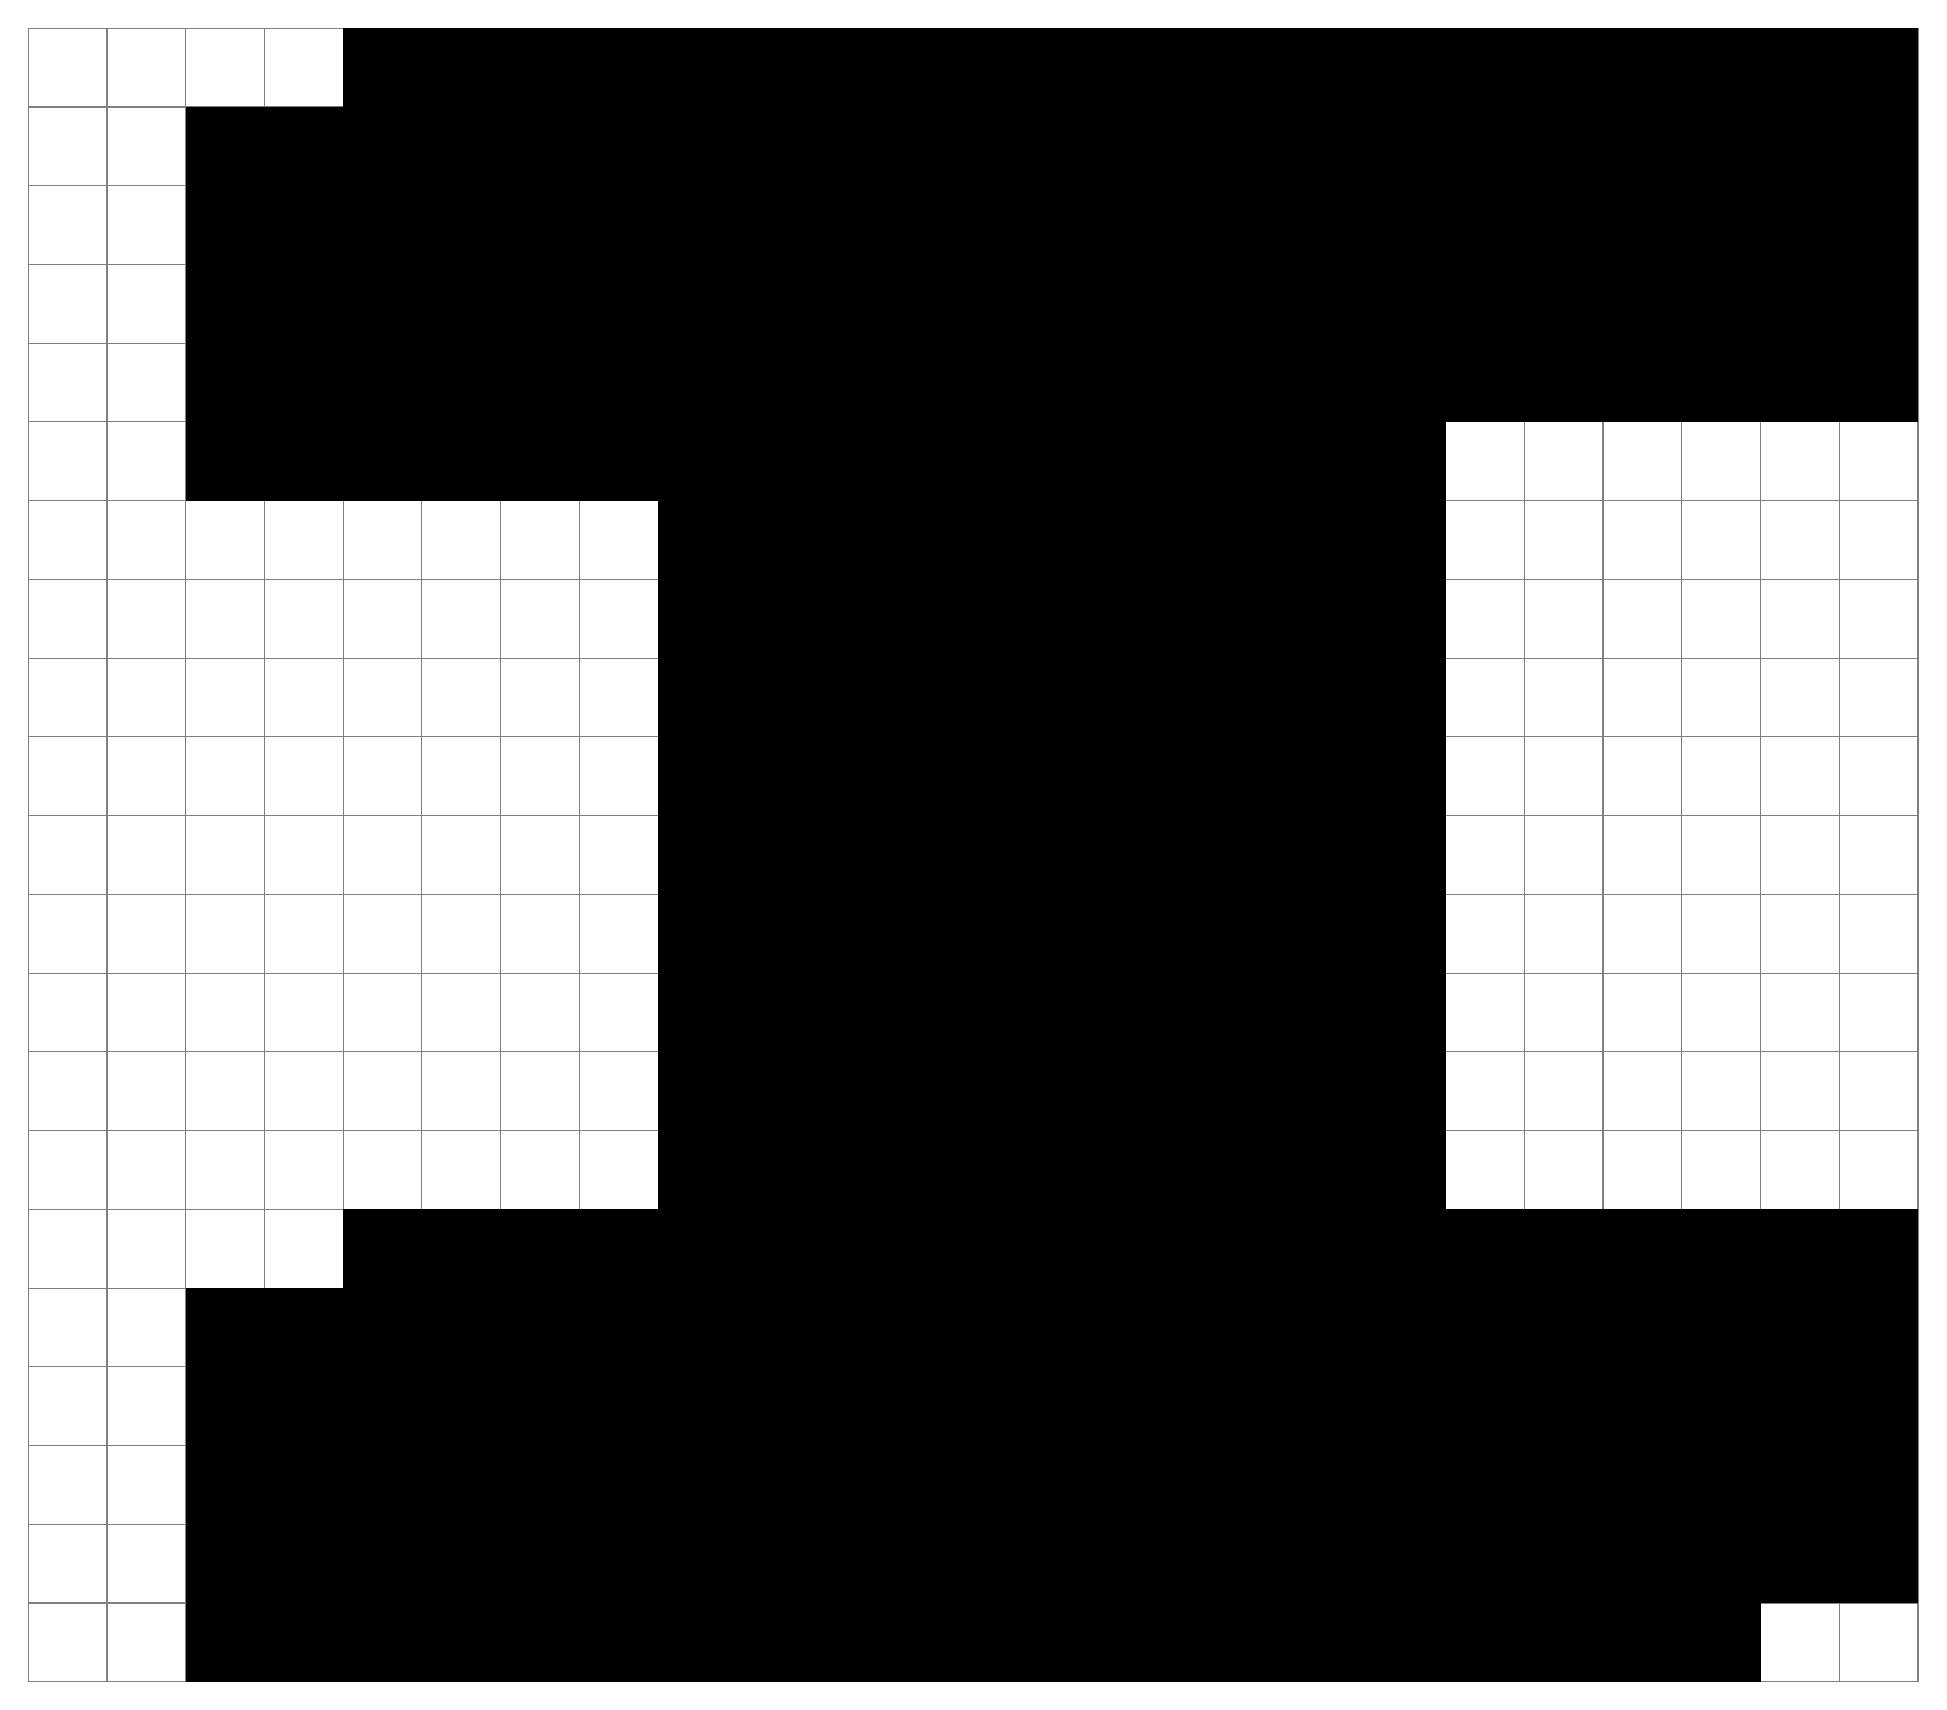
\begin{tikzpicture}

	\draw[step=1.0,gray,thin] (0,0) grid (24,21);
	\fill[\MULTICOLORTWO] (4,20) rectangle ++ (1,1);
	\fill[\MULTICOLORTWO] (5,20) rectangle ++ (1,1);
	\fill[\MULTICOLORTWO] (6,20) rectangle ++ (1,1);
	\fill[\MULTICOLORTWO] (7,20) rectangle ++ (1,1);
	\fill[\MULTICOLORTWO] (8,20) rectangle ++ (1,1);
	\fill[\MULTICOLORTWO] (9,20) rectangle ++ (1,1);
	\fill[\MULTICOLORTWO] (10,20) rectangle ++ (1,1);
	\fill[\MULTICOLORTWO] (11,20) rectangle ++ (1,1);
	\fill[\MULTICOLORTWO] (12,20) rectangle ++ (1,1);
	\fill[\MULTICOLORTWO] (13,20) rectangle ++ (1,1);
	\fill[\MULTICOLORTWO] (14,20) rectangle ++ (1,1);
	\fill[\MULTICOLORTWO] (15,20) rectangle ++ (1,1);
	\fill[\MULTICOLORTWO] (16,20) rectangle ++ (1,1);
	\fill[\MULTICOLORTWO] (17,20) rectangle ++ (1,1);
	\fill[\MULTICOLORTWO] (18,20) rectangle ++ (1,1);
	\fill[\MULTICOLORTWO] (19,20) rectangle ++ (1,1);
	\fill[\MULTICOLORTWO] (20,20) rectangle ++ (1,1);
	\fill[\MULTICOLORTWO] (21,20) rectangle ++ (1,1);
	\fill[\MULTICOLORTWO] (22,20) rectangle ++ (1,1);
	\fill[\MULTICOLORTWO] (23,20) rectangle ++ (1,1);
	\fill[\MULTICOLORONE] (2,19) rectangle ++ (1,1);
	\fill[\MULTICOLORONE] (3,19) rectangle ++ (1,1);
	\fill[\MULTICOLORTWO] (4,19) rectangle ++ (1,1);
	\fill[\MULTICOLORTWO] (5,19) rectangle ++ (1,1);
	\fill[\SPRITECOLOR] (6,19) rectangle ++ (1,1);
	\fill[\SPRITECOLOR] (7,19) rectangle ++ (1,1);
	\fill[\SPRITECOLOR] (8,19) rectangle ++ (1,1);
	\fill[\SPRITECOLOR] (9,19) rectangle ++ (1,1);
	\fill[\SPRITECOLOR] (10,19) rectangle ++ (1,1);
	\fill[\SPRITECOLOR] (11,19) rectangle ++ (1,1);
	\fill[\SPRITECOLOR] (12,19) rectangle ++ (1,1);
	\fill[\SPRITECOLOR] (13,19) rectangle ++ (1,1);
	\fill[\SPRITECOLOR] (14,19) rectangle ++ (1,1);
	\fill[\SPRITECOLOR] (15,19) rectangle ++ (1,1);
	\fill[\SPRITECOLOR] (16,19) rectangle ++ (1,1);
	\fill[\SPRITECOLOR] (17,19) rectangle ++ (1,1);
	\fill[\SPRITECOLOR] (18,19) rectangle ++ (1,1);
	\fill[\SPRITECOLOR] (19,19) rectangle ++ (1,1);
	\fill[\SPRITECOLOR] (20,19) rectangle ++ (1,1);
	\fill[\SPRITECOLOR] (21,19) rectangle ++ (1,1);
	\fill[\MULTICOLORTWO] (22,19) rectangle ++ (1,1);
	\fill[\MULTICOLORTWO] (23,19) rectangle ++ (1,1);
	\fill[\MULTICOLORONE] (2,18) rectangle ++ (1,1);
	\fill[\MULTICOLORONE] (3,18) rectangle ++ (1,1);
	\fill[\MULTICOLORTWO] (4,18) rectangle ++ (1,1);
	\fill[\MULTICOLORTWO] (5,18) rectangle ++ (1,1);
	\fill[\SPRITECOLOR] (6,18) rectangle ++ (1,1);
	\fill[\SPRITECOLOR] (7,18) rectangle ++ (1,1);
	\fill[\SPRITECOLOR] (8,18) rectangle ++ (1,1);
	\fill[\SPRITECOLOR] (9,18) rectangle ++ (1,1);
	\fill[\SPRITECOLOR] (10,18) rectangle ++ (1,1);
	\fill[\SPRITECOLOR] (11,18) rectangle ++ (1,1);
	\fill[\SPRITECOLOR] (12,18) rectangle ++ (1,1);
	\fill[\SPRITECOLOR] (13,18) rectangle ++ (1,1);
	\fill[\SPRITECOLOR] (14,18) rectangle ++ (1,1);
	\fill[\SPRITECOLOR] (15,18) rectangle ++ (1,1);
	\fill[\SPRITECOLOR] (16,18) rectangle ++ (1,1);
	\fill[\SPRITECOLOR] (17,18) rectangle ++ (1,1);
	\fill[\SPRITECOLOR] (18,18) rectangle ++ (1,1);
	\fill[\SPRITECOLOR] (19,18) rectangle ++ (1,1);
	\fill[\SPRITECOLOR] (20,18) rectangle ++ (1,1);
	\fill[\SPRITECOLOR] (21,18) rectangle ++ (1,1);
	\fill[\MULTICOLORTWO] (22,18) rectangle ++ (1,1);
	\fill[\MULTICOLORTWO] (23,18) rectangle ++ (1,1);
	\fill[\MULTICOLORONE] (2,17) rectangle ++ (1,1);
	\fill[\MULTICOLORONE] (3,17) rectangle ++ (1,1);
	\fill[\MULTICOLORTWO] (4,17) rectangle ++ (1,1);
	\fill[\MULTICOLORTWO] (5,17) rectangle ++ (1,1);
	\fill[\SPRITECOLOR] (6,17) rectangle ++ (1,1);
	\fill[\SPRITECOLOR] (7,17) rectangle ++ (1,1);
	\fill[\SPRITECOLOR] (8,17) rectangle ++ (1,1);
	\fill[\SPRITECOLOR] (9,17) rectangle ++ (1,1);
	\fill[\SPRITECOLOR] (10,17) rectangle ++ (1,1);
	\fill[\SPRITECOLOR] (11,17) rectangle ++ (1,1);
	\fill[\SPRITECOLOR] (12,17) rectangle ++ (1,1);
	\fill[\SPRITECOLOR] (13,17) rectangle ++ (1,1);
	\fill[\SPRITECOLOR] (14,17) rectangle ++ (1,1);
	\fill[\SPRITECOLOR] (15,17) rectangle ++ (1,1);
	\fill[\SPRITECOLOR] (16,17) rectangle ++ (1,1);
	\fill[\SPRITECOLOR] (17,17) rectangle ++ (1,1);
	\fill[\SPRITECOLOR] (18,17) rectangle ++ (1,1);
	\fill[\SPRITECOLOR] (19,17) rectangle ++ (1,1);
	\fill[\SPRITECOLOR] (20,17) rectangle ++ (1,1);
	\fill[\SPRITECOLOR] (21,17) rectangle ++ (1,1);
	\fill[\MULTICOLORTWO] (22,17) rectangle ++ (1,1);
	\fill[\MULTICOLORTWO] (23,17) rectangle ++ (1,1);
	\fill[\MULTICOLORONE] (2,16) rectangle ++ (1,1);
	\fill[\MULTICOLORONE] (3,16) rectangle ++ (1,1);
	\fill[\MULTICOLORTWO] (4,16) rectangle ++ (1,1);
	\fill[\MULTICOLORTWO] (5,16) rectangle ++ (1,1);
	\fill[\MULTICOLORTWO] (6,16) rectangle ++ (1,1);
	\fill[\MULTICOLORTWO] (7,16) rectangle ++ (1,1);
	\fill[\MULTICOLORTWO] (8,16) rectangle ++ (1,1);
	\fill[\MULTICOLORTWO] (9,16) rectangle ++ (1,1);
	\fill[\MULTICOLORTWO] (10,16) rectangle ++ (1,1);
	\fill[\MULTICOLORTWO] (11,16) rectangle ++ (1,1);
	\fill[\SPRITECOLOR] (12,16) rectangle ++ (1,1);
	\fill[\SPRITECOLOR] (13,16) rectangle ++ (1,1);
	\fill[\SPRITECOLOR] (14,16) rectangle ++ (1,1);
	\fill[\SPRITECOLOR] (15,16) rectangle ++ (1,1);
	\fill[\MULTICOLORTWO] (16,16) rectangle ++ (1,1);
	\fill[\MULTICOLORTWO] (17,16) rectangle ++ (1,1);
	\fill[\MULTICOLORTWO] (18,16) rectangle ++ (1,1);
	\fill[\MULTICOLORTWO] (19,16) rectangle ++ (1,1);
	\fill[\MULTICOLORTWO] (20,16) rectangle ++ (1,1);
	\fill[\MULTICOLORTWO] (21,16) rectangle ++ (1,1);
	\fill[\MULTICOLORTWO] (22,16) rectangle ++ (1,1);
	\fill[\MULTICOLORTWO] (23,16) rectangle ++ (1,1);
	\fill[\MULTICOLORONE] (2,15) rectangle ++ (1,1);
	\fill[\MULTICOLORONE] (3,15) rectangle ++ (1,1);
	\fill[\MULTICOLORONE] (4,15) rectangle ++ (1,1);
	\fill[\MULTICOLORONE] (5,15) rectangle ++ (1,1);
	\fill[\MULTICOLORONE] (6,15) rectangle ++ (1,1);
	\fill[\MULTICOLORONE] (7,15) rectangle ++ (1,1);
	\fill[\MULTICOLORONE] (8,15) rectangle ++ (1,1);
	\fill[\MULTICOLORONE] (9,15) rectangle ++ (1,1);
	\fill[\MULTICOLORTWO] (10,15) rectangle ++ (1,1);
	\fill[\MULTICOLORTWO] (11,15) rectangle ++ (1,1);
	\fill[\SPRITECOLOR] (12,15) rectangle ++ (1,1);
	\fill[\SPRITECOLOR] (13,15) rectangle ++ (1,1);
	\fill[\SPRITECOLOR] (14,15) rectangle ++ (1,1);
	\fill[\SPRITECOLOR] (15,15) rectangle ++ (1,1);
	\fill[\MULTICOLORTWO] (16,15) rectangle ++ (1,1);
	\fill[\MULTICOLORTWO] (17,15) rectangle ++ (1,1);
	\fill[\MULTICOLORONE] (8,14) rectangle ++ (1,1);
	\fill[\MULTICOLORONE] (9,14) rectangle ++ (1,1);
	\fill[\MULTICOLORTWO] (10,14) rectangle ++ (1,1);
	\fill[\MULTICOLORTWO] (11,14) rectangle ++ (1,1);
	\fill[\SPRITECOLOR] (12,14) rectangle ++ (1,1);
	\fill[\SPRITECOLOR] (13,14) rectangle ++ (1,1);
	\fill[\SPRITECOLOR] (14,14) rectangle ++ (1,1);
	\fill[\SPRITECOLOR] (15,14) rectangle ++ (1,1);
	\fill[\MULTICOLORTWO] (16,14) rectangle ++ (1,1);
	\fill[\MULTICOLORTWO] (17,14) rectangle ++ (1,1);
	\fill[\MULTICOLORONE] (8,13) rectangle ++ (1,1);
	\fill[\MULTICOLORONE] (9,13) rectangle ++ (1,1);
	\fill[\MULTICOLORTWO] (10,13) rectangle ++ (1,1);
	\fill[\MULTICOLORTWO] (11,13) rectangle ++ (1,1);
	\fill[\SPRITECOLOR] (12,13) rectangle ++ (1,1);
	\fill[\SPRITECOLOR] (13,13) rectangle ++ (1,1);
	\fill[\SPRITECOLOR] (14,13) rectangle ++ (1,1);
	\fill[\SPRITECOLOR] (15,13) rectangle ++ (1,1);
	\fill[\MULTICOLORTWO] (16,13) rectangle ++ (1,1);
	\fill[\MULTICOLORTWO] (17,13) rectangle ++ (1,1);
	\fill[\MULTICOLORONE] (8,12) rectangle ++ (1,1);
	\fill[\MULTICOLORONE] (9,12) rectangle ++ (1,1);
	\fill[\MULTICOLORTWO] (10,12) rectangle ++ (1,1);
	\fill[\MULTICOLORTWO] (11,12) rectangle ++ (1,1);
	\fill[\SPRITECOLOR] (12,12) rectangle ++ (1,1);
	\fill[\SPRITECOLOR] (13,12) rectangle ++ (1,1);
	\fill[\SPRITECOLOR] (14,12) rectangle ++ (1,1);
	\fill[\SPRITECOLOR] (15,12) rectangle ++ (1,1);
	\fill[\MULTICOLORTWO] (16,12) rectangle ++ (1,1);
	\fill[\MULTICOLORTWO] (17,12) rectangle ++ (1,1);
	\fill[\MULTICOLORONE] (8,11) rectangle ++ (1,1);
	\fill[\MULTICOLORONE] (9,11) rectangle ++ (1,1);
	\fill[\MULTICOLORTWO] (10,11) rectangle ++ (1,1);
	\fill[\MULTICOLORTWO] (11,11) rectangle ++ (1,1);
	\fill[\SPRITECOLOR] (12,11) rectangle ++ (1,1);
	\fill[\SPRITECOLOR] (13,11) rectangle ++ (1,1);
	\fill[\SPRITECOLOR] (14,11) rectangle ++ (1,1);
	\fill[\SPRITECOLOR] (15,11) rectangle ++ (1,1);
	\fill[\MULTICOLORTWO] (16,11) rectangle ++ (1,1);
	\fill[\MULTICOLORTWO] (17,11) rectangle ++ (1,1);
	\fill[\MULTICOLORONE] (8,10) rectangle ++ (1,1);
	\fill[\MULTICOLORONE] (9,10) rectangle ++ (1,1);
	\fill[\MULTICOLORTWO] (10,10) rectangle ++ (1,1);
	\fill[\MULTICOLORTWO] (11,10) rectangle ++ (1,1);
	\fill[\SPRITECOLOR] (12,10) rectangle ++ (1,1);
	\fill[\SPRITECOLOR] (13,10) rectangle ++ (1,1);
	\fill[\SPRITECOLOR] (14,10) rectangle ++ (1,1);
	\fill[\SPRITECOLOR] (15,10) rectangle ++ (1,1);
	\fill[\MULTICOLORTWO] (16,10) rectangle ++ (1,1);
	\fill[\MULTICOLORTWO] (17,10) rectangle ++ (1,1);
	\fill[\MULTICOLORONE] (8,9) rectangle ++ (1,1);
	\fill[\MULTICOLORONE] (9,9) rectangle ++ (1,1);
	\fill[\MULTICOLORTWO] (10,9) rectangle ++ (1,1);
	\fill[\MULTICOLORTWO] (11,9) rectangle ++ (1,1);
	\fill[\SPRITECOLOR] (12,9) rectangle ++ (1,1);
	\fill[\SPRITECOLOR] (13,9) rectangle ++ (1,1);
	\fill[\SPRITECOLOR] (14,9) rectangle ++ (1,1);
	\fill[\SPRITECOLOR] (15,9) rectangle ++ (1,1);
	\fill[\MULTICOLORTWO] (16,9) rectangle ++ (1,1);
	\fill[\MULTICOLORTWO] (17,9) rectangle ++ (1,1);
	\fill[\MULTICOLORONE] (8,8) rectangle ++ (1,1);
	\fill[\MULTICOLORONE] (9,8) rectangle ++ (1,1);
	\fill[\MULTICOLORTWO] (10,8) rectangle ++ (1,1);
	\fill[\MULTICOLORTWO] (11,8) rectangle ++ (1,1);
	\fill[\SPRITECOLOR] (12,8) rectangle ++ (1,1);
	\fill[\SPRITECOLOR] (13,8) rectangle ++ (1,1);
	\fill[\SPRITECOLOR] (14,8) rectangle ++ (1,1);
	\fill[\SPRITECOLOR] (15,8) rectangle ++ (1,1);
	\fill[\MULTICOLORTWO] (16,8) rectangle ++ (1,1);
	\fill[\MULTICOLORTWO] (17,8) rectangle ++ (1,1);
	\fill[\MULTICOLORONE] (8,7) rectangle ++ (1,1);
	\fill[\MULTICOLORONE] (9,7) rectangle ++ (1,1);
	\fill[\MULTICOLORTWO] (10,7) rectangle ++ (1,1);
	\fill[\MULTICOLORTWO] (11,7) rectangle ++ (1,1);
	\fill[\SPRITECOLOR] (12,7) rectangle ++ (1,1);
	\fill[\SPRITECOLOR] (13,7) rectangle ++ (1,1);
	\fill[\SPRITECOLOR] (14,7) rectangle ++ (1,1);
	\fill[\SPRITECOLOR] (15,7) rectangle ++ (1,1);
	\fill[\MULTICOLORTWO] (16,7) rectangle ++ (1,1);
	\fill[\MULTICOLORTWO] (17,7) rectangle ++ (1,1);
	\fill[\MULTICOLORONE] (8,6) rectangle ++ (1,1);
	\fill[\MULTICOLORONE] (9,6) rectangle ++ (1,1);
	\fill[\MULTICOLORTWO] (10,6) rectangle ++ (1,1);
	\fill[\MULTICOLORTWO] (11,6) rectangle ++ (1,1);
	\fill[\SPRITECOLOR] (12,6) rectangle ++ (1,1);
	\fill[\SPRITECOLOR] (13,6) rectangle ++ (1,1);
	\fill[\SPRITECOLOR] (14,6) rectangle ++ (1,1);
	\fill[\SPRITECOLOR] (15,6) rectangle ++ (1,1);
	\fill[\MULTICOLORTWO] (16,6) rectangle ++ (1,1);
	\fill[\MULTICOLORTWO] (17,6) rectangle ++ (1,1);
	\fill[\MULTICOLORTWO] (4,5) rectangle ++ (1,1);
	\fill[\MULTICOLORTWO] (5,5) rectangle ++ (1,1);
	\fill[\MULTICOLORTWO] (6,5) rectangle ++ (1,1);
	\fill[\MULTICOLORTWO] (7,5) rectangle ++ (1,1);
	\fill[\MULTICOLORTWO] (8,5) rectangle ++ (1,1);
	\fill[\MULTICOLORTWO] (9,5) rectangle ++ (1,1);
	\fill[\MULTICOLORTWO] (10,5) rectangle ++ (1,1);
	\fill[\MULTICOLORTWO] (11,5) rectangle ++ (1,1);
	\fill[\SPRITECOLOR] (12,5) rectangle ++ (1,1);
	\fill[\SPRITECOLOR] (13,5) rectangle ++ (1,1);
	\fill[\SPRITECOLOR] (14,5) rectangle ++ (1,1);
	\fill[\SPRITECOLOR] (15,5) rectangle ++ (1,1);
	\fill[\MULTICOLORTWO] (16,5) rectangle ++ (1,1);
	\fill[\MULTICOLORTWO] (17,5) rectangle ++ (1,1);
	\fill[\MULTICOLORTWO] (18,5) rectangle ++ (1,1);
	\fill[\MULTICOLORTWO] (19,5) rectangle ++ (1,1);
	\fill[\MULTICOLORTWO] (20,5) rectangle ++ (1,1);
	\fill[\MULTICOLORTWO] (21,5) rectangle ++ (1,1);
	\fill[\MULTICOLORTWO] (22,5) rectangle ++ (1,1);
	\fill[\MULTICOLORTWO] (23,5) rectangle ++ (1,1);
	\fill[\MULTICOLORONE] (2,4) rectangle ++ (1,1);
	\fill[\MULTICOLORONE] (3,4) rectangle ++ (1,1);
	\fill[\MULTICOLORTWO] (4,4) rectangle ++ (1,1);
	\fill[\MULTICOLORTWO] (5,4) rectangle ++ (1,1);
	\fill[\SPRITECOLOR] (6,4) rectangle ++ (1,1);
	\fill[\SPRITECOLOR] (7,4) rectangle ++ (1,1);
	\fill[\SPRITECOLOR] (8,4) rectangle ++ (1,1);
	\fill[\SPRITECOLOR] (9,4) rectangle ++ (1,1);
	\fill[\SPRITECOLOR] (10,4) rectangle ++ (1,1);
	\fill[\SPRITECOLOR] (11,4) rectangle ++ (1,1);
	\fill[\SPRITECOLOR] (12,4) rectangle ++ (1,1);
	\fill[\SPRITECOLOR] (13,4) rectangle ++ (1,1);
	\fill[\SPRITECOLOR] (14,4) rectangle ++ (1,1);
	\fill[\SPRITECOLOR] (15,4) rectangle ++ (1,1);
	\fill[\SPRITECOLOR] (16,4) rectangle ++ (1,1);
	\fill[\SPRITECOLOR] (17,4) rectangle ++ (1,1);
	\fill[\SPRITECOLOR] (18,4) rectangle ++ (1,1);
	\fill[\SPRITECOLOR] (19,4) rectangle ++ (1,1);
	\fill[\SPRITECOLOR] (20,4) rectangle ++ (1,1);
	\fill[\SPRITECOLOR] (21,4) rectangle ++ (1,1);
	\fill[\MULTICOLORTWO] (22,4) rectangle ++ (1,1);
	\fill[\MULTICOLORTWO] (23,4) rectangle ++ (1,1);
	\fill[\MULTICOLORONE] (2,3) rectangle ++ (1,1);
	\fill[\MULTICOLORONE] (3,3) rectangle ++ (1,1);
	\fill[\MULTICOLORTWO] (4,3) rectangle ++ (1,1);
	\fill[\MULTICOLORTWO] (5,3) rectangle ++ (1,1);
	\fill[\SPRITECOLOR] (6,3) rectangle ++ (1,1);
	\fill[\SPRITECOLOR] (7,3) rectangle ++ (1,1);
	\fill[\SPRITECOLOR] (8,3) rectangle ++ (1,1);
	\fill[\SPRITECOLOR] (9,3) rectangle ++ (1,1);
	\fill[\SPRITECOLOR] (10,3) rectangle ++ (1,1);
	\fill[\SPRITECOLOR] (11,3) rectangle ++ (1,1);
	\fill[\SPRITECOLOR] (12,3) rectangle ++ (1,1);
	\fill[\SPRITECOLOR] (13,3) rectangle ++ (1,1);
	\fill[\SPRITECOLOR] (14,3) rectangle ++ (1,1);
	\fill[\SPRITECOLOR] (15,3) rectangle ++ (1,1);
	\fill[\SPRITECOLOR] (16,3) rectangle ++ (1,1);
	\fill[\SPRITECOLOR] (17,3) rectangle ++ (1,1);
	\fill[\SPRITECOLOR] (18,3) rectangle ++ (1,1);
	\fill[\SPRITECOLOR] (19,3) rectangle ++ (1,1);
	\fill[\SPRITECOLOR] (20,3) rectangle ++ (1,1);
	\fill[\SPRITECOLOR] (21,3) rectangle ++ (1,1);
	\fill[\MULTICOLORTWO] (22,3) rectangle ++ (1,1);
	\fill[\MULTICOLORTWO] (23,3) rectangle ++ (1,1);
	\fill[\MULTICOLORONE] (2,2) rectangle ++ (1,1);
	\fill[\MULTICOLORONE] (3,2) rectangle ++ (1,1);
	\fill[\MULTICOLORTWO] (4,2) rectangle ++ (1,1);
	\fill[\MULTICOLORTWO] (5,2) rectangle ++ (1,1);
	\fill[\SPRITECOLOR] (6,2) rectangle ++ (1,1);
	\fill[\SPRITECOLOR] (7,2) rectangle ++ (1,1);
	\fill[\SPRITECOLOR] (8,2) rectangle ++ (1,1);
	\fill[\SPRITECOLOR] (9,2) rectangle ++ (1,1);
	\fill[\SPRITECOLOR] (10,2) rectangle ++ (1,1);
	\fill[\SPRITECOLOR] (11,2) rectangle ++ (1,1);
	\fill[\SPRITECOLOR] (12,2) rectangle ++ (1,1);
	\fill[\SPRITECOLOR] (13,2) rectangle ++ (1,1);
	\fill[\SPRITECOLOR] (14,2) rectangle ++ (1,1);
	\fill[\SPRITECOLOR] (15,2) rectangle ++ (1,1);
	\fill[\SPRITECOLOR] (16,2) rectangle ++ (1,1);
	\fill[\SPRITECOLOR] (17,2) rectangle ++ (1,1);
	\fill[\SPRITECOLOR] (18,2) rectangle ++ (1,1);
	\fill[\SPRITECOLOR] (19,2) rectangle ++ (1,1);
	\fill[\SPRITECOLOR] (20,2) rectangle ++ (1,1);
	\fill[\SPRITECOLOR] (21,2) rectangle ++ (1,1);
	\fill[\MULTICOLORTWO] (22,2) rectangle ++ (1,1);
	\fill[\MULTICOLORTWO] (23,2) rectangle ++ (1,1);
	\fill[\MULTICOLORONE] (2,1) rectangle ++ (1,1);
	\fill[\MULTICOLORONE] (3,1) rectangle ++ (1,1);
	\fill[\MULTICOLORTWO] (4,1) rectangle ++ (1,1);
	\fill[\MULTICOLORTWO] (5,1) rectangle ++ (1,1);
	\fill[\MULTICOLORTWO] (6,1) rectangle ++ (1,1);
	\fill[\MULTICOLORTWO] (7,1) rectangle ++ (1,1);
	\fill[\MULTICOLORTWO] (8,1) rectangle ++ (1,1);
	\fill[\MULTICOLORTWO] (9,1) rectangle ++ (1,1);
	\fill[\MULTICOLORTWO] (10,1) rectangle ++ (1,1);
	\fill[\MULTICOLORTWO] (11,1) rectangle ++ (1,1);
	\fill[\MULTICOLORTWO] (12,1) rectangle ++ (1,1);
	\fill[\MULTICOLORTWO] (13,1) rectangle ++ (1,1);
	\fill[\MULTICOLORTWO] (14,1) rectangle ++ (1,1);
	\fill[\MULTICOLORTWO] (15,1) rectangle ++ (1,1);
	\fill[\MULTICOLORTWO] (16,1) rectangle ++ (1,1);
	\fill[\MULTICOLORTWO] (17,1) rectangle ++ (1,1);
	\fill[\MULTICOLORTWO] (18,1) rectangle ++ (1,1);
	\fill[\MULTICOLORTWO] (19,1) rectangle ++ (1,1);
	\fill[\MULTICOLORTWO] (20,1) rectangle ++ (1,1);
	\fill[\MULTICOLORTWO] (21,1) rectangle ++ (1,1);
	\fill[\MULTICOLORTWO] (22,1) rectangle ++ (1,1);
	\fill[\MULTICOLORTWO] (23,1) rectangle ++ (1,1);
	\fill[\MULTICOLORONE] (2,0) rectangle ++ (1,1);
	\fill[\MULTICOLORONE] (3,0) rectangle ++ (1,1);
	\fill[\MULTICOLORONE] (4,0) rectangle ++ (1,1);
	\fill[\MULTICOLORONE] (5,0) rectangle ++ (1,1);
	\fill[\MULTICOLORONE] (6,0) rectangle ++ (1,1);
	\fill[\MULTICOLORONE] (7,0) rectangle ++ (1,1);
	\fill[\MULTICOLORONE] (8,0) rectangle ++ (1,1);
	\fill[\MULTICOLORONE] (9,0) rectangle ++ (1,1);
	\fill[\MULTICOLORONE] (10,0) rectangle ++ (1,1);
	\fill[\MULTICOLORONE] (11,0) rectangle ++ (1,1);
	\fill[\MULTICOLORONE] (12,0) rectangle ++ (1,1);
	\fill[\MULTICOLORONE] (13,0) rectangle ++ (1,1);
	\fill[\MULTICOLORONE] (14,0) rectangle ++ (1,1);
	\fill[\MULTICOLORONE] (15,0) rectangle ++ (1,1);
	\fill[\MULTICOLORONE] (16,0) rectangle ++ (1,1);
	\fill[\MULTICOLORONE] (17,0) rectangle ++ (1,1);
	\fill[\MULTICOLORONE] (18,0) rectangle ++ (1,1);
	\fill[\MULTICOLORONE] (19,0) rectangle ++ (1,1);
	\fill[\MULTICOLORONE] (20,0) rectangle ++ (1,1);
	\fill[\MULTICOLORONE] (21,0) rectangle ++ (1,1);

      \end{tikzpicture}
    \end{adjustbox}
  }\caption{BIG\_I}
\end{figure}

	\end{subfigure}
} &
\makecell[l]{
	\begin{subfigure}{0.3\textwidth}
    \def\MULTICOLORONE{gray}
    \def\MULTICOLORTWO{black}
    \def\SPRITECOLOR{purple}
		
\begin{figure}[H]
  {
    \setlength{\tabcolsep}{3.0pt}
    \setlength\cmidrulewidth{\heavyrulewidth} % Make cmidrule = 
    \begin{adjustbox}{width=3cm,center}
      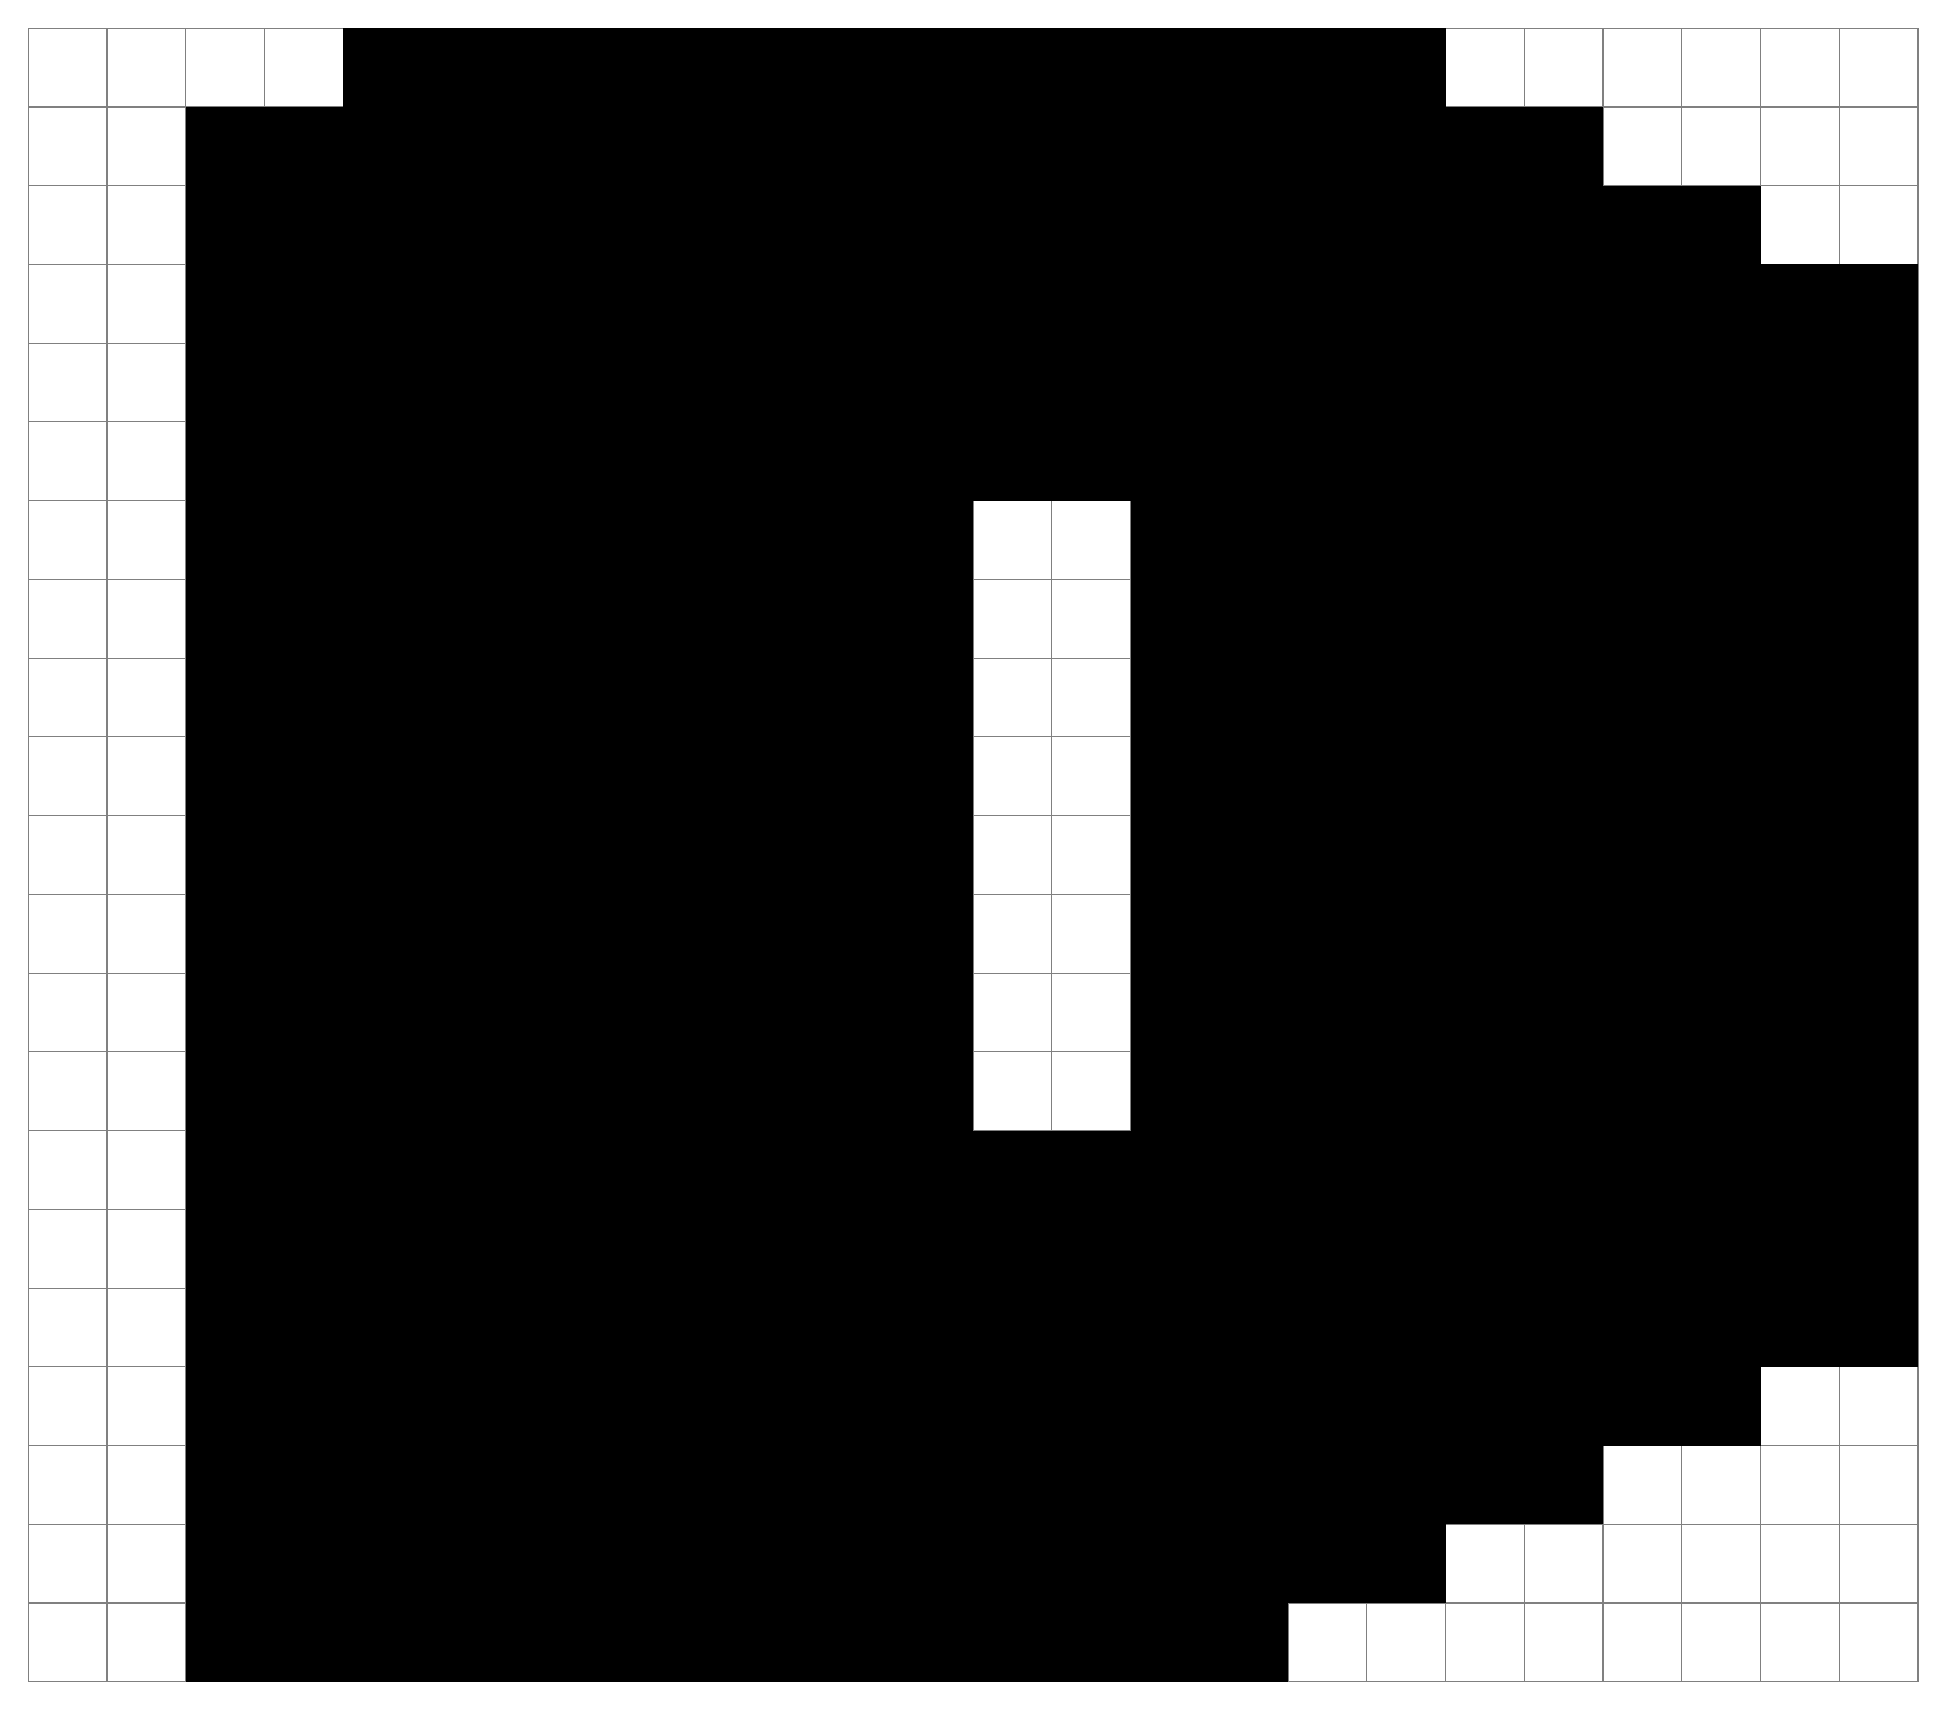
\begin{tikzpicture}

	\draw[step=1.0,gray,thin] (0,0) grid (24,21);
	\fill[\MULTICOLORTWO] (4,20) rectangle ++ (1,1);
	\fill[\MULTICOLORTWO] (5,20) rectangle ++ (1,1);
	\fill[\MULTICOLORTWO] (6,20) rectangle ++ (1,1);
	\fill[\MULTICOLORTWO] (7,20) rectangle ++ (1,1);
	\fill[\MULTICOLORTWO] (8,20) rectangle ++ (1,1);
	\fill[\MULTICOLORTWO] (9,20) rectangle ++ (1,1);
	\fill[\MULTICOLORTWO] (10,20) rectangle ++ (1,1);
	\fill[\MULTICOLORTWO] (11,20) rectangle ++ (1,1);
	\fill[\MULTICOLORTWO] (12,20) rectangle ++ (1,1);
	\fill[\MULTICOLORTWO] (13,20) rectangle ++ (1,1);
	\fill[\MULTICOLORTWO] (14,20) rectangle ++ (1,1);
	\fill[\MULTICOLORTWO] (15,20) rectangle ++ (1,1);
	\fill[\MULTICOLORTWO] (16,20) rectangle ++ (1,1);
	\fill[\MULTICOLORTWO] (17,20) rectangle ++ (1,1);
	\fill[\MULTICOLORONE] (2,19) rectangle ++ (1,1);
	\fill[\MULTICOLORONE] (3,19) rectangle ++ (1,1);
	\fill[\MULTICOLORTWO] (4,19) rectangle ++ (1,1);
	\fill[\MULTICOLORTWO] (5,19) rectangle ++ (1,1);
	\fill[\SPRITECOLOR] (6,19) rectangle ++ (1,1);
	\fill[\SPRITECOLOR] (7,19) rectangle ++ (1,1);
	\fill[\SPRITECOLOR] (8,19) rectangle ++ (1,1);
	\fill[\SPRITECOLOR] (9,19) rectangle ++ (1,1);
	\fill[\SPRITECOLOR] (10,19) rectangle ++ (1,1);
	\fill[\SPRITECOLOR] (11,19) rectangle ++ (1,1);
	\fill[\SPRITECOLOR] (12,19) rectangle ++ (1,1);
	\fill[\SPRITECOLOR] (13,19) rectangle ++ (1,1);
	\fill[\SPRITECOLOR] (14,19) rectangle ++ (1,1);
	\fill[\SPRITECOLOR] (15,19) rectangle ++ (1,1);
	\fill[\SPRITECOLOR] (16,19) rectangle ++ (1,1);
	\fill[\SPRITECOLOR] (17,19) rectangle ++ (1,1);
	\fill[\MULTICOLORTWO] (18,19) rectangle ++ (1,1);
	\fill[\MULTICOLORTWO] (19,19) rectangle ++ (1,1);
	\fill[\MULTICOLORONE] (2,18) rectangle ++ (1,1);
	\fill[\MULTICOLORONE] (3,18) rectangle ++ (1,1);
	\fill[\MULTICOLORTWO] (4,18) rectangle ++ (1,1);
	\fill[\MULTICOLORTWO] (5,18) rectangle ++ (1,1);
	\fill[\SPRITECOLOR] (6,18) rectangle ++ (1,1);
	\fill[\SPRITECOLOR] (7,18) rectangle ++ (1,1);
	\fill[\SPRITECOLOR] (8,18) rectangle ++ (1,1);
	\fill[\SPRITECOLOR] (9,18) rectangle ++ (1,1);
	\fill[\SPRITECOLOR] (10,18) rectangle ++ (1,1);
	\fill[\SPRITECOLOR] (11,18) rectangle ++ (1,1);
	\fill[\SPRITECOLOR] (12,18) rectangle ++ (1,1);
	\fill[\SPRITECOLOR] (13,18) rectangle ++ (1,1);
	\fill[\SPRITECOLOR] (14,18) rectangle ++ (1,1);
	\fill[\SPRITECOLOR] (15,18) rectangle ++ (1,1);
	\fill[\SPRITECOLOR] (16,18) rectangle ++ (1,1);
	\fill[\SPRITECOLOR] (17,18) rectangle ++ (1,1);
	\fill[\SPRITECOLOR] (18,18) rectangle ++ (1,1);
	\fill[\SPRITECOLOR] (19,18) rectangle ++ (1,1);
	\fill[\MULTICOLORTWO] (20,18) rectangle ++ (1,1);
	\fill[\MULTICOLORTWO] (21,18) rectangle ++ (1,1);
	\fill[\MULTICOLORONE] (2,17) rectangle ++ (1,1);
	\fill[\MULTICOLORONE] (3,17) rectangle ++ (1,1);
	\fill[\MULTICOLORTWO] (4,17) rectangle ++ (1,1);
	\fill[\MULTICOLORTWO] (5,17) rectangle ++ (1,1);
	\fill[\SPRITECOLOR] (6,17) rectangle ++ (1,1);
	\fill[\SPRITECOLOR] (7,17) rectangle ++ (1,1);
	\fill[\SPRITECOLOR] (8,17) rectangle ++ (1,1);
	\fill[\SPRITECOLOR] (9,17) rectangle ++ (1,1);
	\fill[\SPRITECOLOR] (10,17) rectangle ++ (1,1);
	\fill[\SPRITECOLOR] (11,17) rectangle ++ (1,1);
	\fill[\SPRITECOLOR] (12,17) rectangle ++ (1,1);
	\fill[\SPRITECOLOR] (13,17) rectangle ++ (1,1);
	\fill[\SPRITECOLOR] (14,17) rectangle ++ (1,1);
	\fill[\SPRITECOLOR] (15,17) rectangle ++ (1,1);
	\fill[\SPRITECOLOR] (16,17) rectangle ++ (1,1);
	\fill[\SPRITECOLOR] (17,17) rectangle ++ (1,1);
	\fill[\SPRITECOLOR] (18,17) rectangle ++ (1,1);
	\fill[\SPRITECOLOR] (19,17) rectangle ++ (1,1);
	\fill[\SPRITECOLOR] (20,17) rectangle ++ (1,1);
	\fill[\SPRITECOLOR] (21,17) rectangle ++ (1,1);
	\fill[\MULTICOLORTWO] (22,17) rectangle ++ (1,1);
	\fill[\MULTICOLORTWO] (23,17) rectangle ++ (1,1);
	\fill[\MULTICOLORONE] (2,16) rectangle ++ (1,1);
	\fill[\MULTICOLORONE] (3,16) rectangle ++ (1,1);
	\fill[\MULTICOLORTWO] (4,16) rectangle ++ (1,1);
	\fill[\MULTICOLORTWO] (5,16) rectangle ++ (1,1);
	\fill[\SPRITECOLOR] (6,16) rectangle ++ (1,1);
	\fill[\SPRITECOLOR] (7,16) rectangle ++ (1,1);
	\fill[\SPRITECOLOR] (8,16) rectangle ++ (1,1);
	\fill[\SPRITECOLOR] (9,16) rectangle ++ (1,1);
	\fill[\MULTICOLORTWO] (10,16) rectangle ++ (1,1);
	\fill[\MULTICOLORTWO] (11,16) rectangle ++ (1,1);
	\fill[\MULTICOLORTWO] (12,16) rectangle ++ (1,1);
	\fill[\MULTICOLORTWO] (13,16) rectangle ++ (1,1);
	\fill[\SPRITECOLOR] (14,16) rectangle ++ (1,1);
	\fill[\SPRITECOLOR] (15,16) rectangle ++ (1,1);
	\fill[\SPRITECOLOR] (16,16) rectangle ++ (1,1);
	\fill[\SPRITECOLOR] (17,16) rectangle ++ (1,1);
	\fill[\SPRITECOLOR] (18,16) rectangle ++ (1,1);
	\fill[\SPRITECOLOR] (19,16) rectangle ++ (1,1);
	\fill[\SPRITECOLOR] (20,16) rectangle ++ (1,1);
	\fill[\SPRITECOLOR] (21,16) rectangle ++ (1,1);
	\fill[\MULTICOLORTWO] (22,16) rectangle ++ (1,1);
	\fill[\MULTICOLORTWO] (23,16) rectangle ++ (1,1);
	\fill[\MULTICOLORONE] (2,15) rectangle ++ (1,1);
	\fill[\MULTICOLORONE] (3,15) rectangle ++ (1,1);
	\fill[\MULTICOLORTWO] (4,15) rectangle ++ (1,1);
	\fill[\MULTICOLORTWO] (5,15) rectangle ++ (1,1);
	\fill[\SPRITECOLOR] (6,15) rectangle ++ (1,1);
	\fill[\SPRITECOLOR] (7,15) rectangle ++ (1,1);
	\fill[\SPRITECOLOR] (8,15) rectangle ++ (1,1);
	\fill[\SPRITECOLOR] (9,15) rectangle ++ (1,1);
	\fill[\MULTICOLORTWO] (10,15) rectangle ++ (1,1);
	\fill[\MULTICOLORTWO] (11,15) rectangle ++ (1,1);
	\fill[\MULTICOLORONE] (12,15) rectangle ++ (1,1);
	\fill[\MULTICOLORONE] (13,15) rectangle ++ (1,1);
	\fill[\MULTICOLORTWO] (14,15) rectangle ++ (1,1);
	\fill[\MULTICOLORTWO] (15,15) rectangle ++ (1,1);
	\fill[\SPRITECOLOR] (16,15) rectangle ++ (1,1);
	\fill[\SPRITECOLOR] (17,15) rectangle ++ (1,1);
	\fill[\SPRITECOLOR] (18,15) rectangle ++ (1,1);
	\fill[\SPRITECOLOR] (19,15) rectangle ++ (1,1);
	\fill[\SPRITECOLOR] (20,15) rectangle ++ (1,1);
	\fill[\SPRITECOLOR] (21,15) rectangle ++ (1,1);
	\fill[\MULTICOLORTWO] (22,15) rectangle ++ (1,1);
	\fill[\MULTICOLORTWO] (23,15) rectangle ++ (1,1);
	\fill[\MULTICOLORONE] (2,14) rectangle ++ (1,1);
	\fill[\MULTICOLORONE] (3,14) rectangle ++ (1,1);
	\fill[\MULTICOLORTWO] (4,14) rectangle ++ (1,1);
	\fill[\MULTICOLORTWO] (5,14) rectangle ++ (1,1);
	\fill[\SPRITECOLOR] (6,14) rectangle ++ (1,1);
	\fill[\SPRITECOLOR] (7,14) rectangle ++ (1,1);
	\fill[\SPRITECOLOR] (8,14) rectangle ++ (1,1);
	\fill[\SPRITECOLOR] (9,14) rectangle ++ (1,1);
	\fill[\MULTICOLORTWO] (10,14) rectangle ++ (1,1);
	\fill[\MULTICOLORTWO] (11,14) rectangle ++ (1,1);
	\fill[\MULTICOLORONE] (14,14) rectangle ++ (1,1);
	\fill[\MULTICOLORONE] (15,14) rectangle ++ (1,1);
	\fill[\MULTICOLORTWO] (16,14) rectangle ++ (1,1);
	\fill[\MULTICOLORTWO] (17,14) rectangle ++ (1,1);
	\fill[\SPRITECOLOR] (18,14) rectangle ++ (1,1);
	\fill[\SPRITECOLOR] (19,14) rectangle ++ (1,1);
	\fill[\SPRITECOLOR] (20,14) rectangle ++ (1,1);
	\fill[\SPRITECOLOR] (21,14) rectangle ++ (1,1);
	\fill[\MULTICOLORTWO] (22,14) rectangle ++ (1,1);
	\fill[\MULTICOLORTWO] (23,14) rectangle ++ (1,1);
	\fill[\MULTICOLORONE] (2,13) rectangle ++ (1,1);
	\fill[\MULTICOLORONE] (3,13) rectangle ++ (1,1);
	\fill[\MULTICOLORTWO] (4,13) rectangle ++ (1,1);
	\fill[\MULTICOLORTWO] (5,13) rectangle ++ (1,1);
	\fill[\SPRITECOLOR] (6,13) rectangle ++ (1,1);
	\fill[\SPRITECOLOR] (7,13) rectangle ++ (1,1);
	\fill[\SPRITECOLOR] (8,13) rectangle ++ (1,1);
	\fill[\SPRITECOLOR] (9,13) rectangle ++ (1,1);
	\fill[\MULTICOLORTWO] (10,13) rectangle ++ (1,1);
	\fill[\MULTICOLORTWO] (11,13) rectangle ++ (1,1);
	\fill[\MULTICOLORONE] (14,13) rectangle ++ (1,1);
	\fill[\MULTICOLORONE] (15,13) rectangle ++ (1,1);
	\fill[\MULTICOLORTWO] (16,13) rectangle ++ (1,1);
	\fill[\MULTICOLORTWO] (17,13) rectangle ++ (1,1);
	\fill[\SPRITECOLOR] (18,13) rectangle ++ (1,1);
	\fill[\SPRITECOLOR] (19,13) rectangle ++ (1,1);
	\fill[\SPRITECOLOR] (20,13) rectangle ++ (1,1);
	\fill[\SPRITECOLOR] (21,13) rectangle ++ (1,1);
	\fill[\MULTICOLORTWO] (22,13) rectangle ++ (1,1);
	\fill[\MULTICOLORTWO] (23,13) rectangle ++ (1,1);
	\fill[\MULTICOLORONE] (2,12) rectangle ++ (1,1);
	\fill[\MULTICOLORONE] (3,12) rectangle ++ (1,1);
	\fill[\MULTICOLORTWO] (4,12) rectangle ++ (1,1);
	\fill[\MULTICOLORTWO] (5,12) rectangle ++ (1,1);
	\fill[\SPRITECOLOR] (6,12) rectangle ++ (1,1);
	\fill[\SPRITECOLOR] (7,12) rectangle ++ (1,1);
	\fill[\SPRITECOLOR] (8,12) rectangle ++ (1,1);
	\fill[\SPRITECOLOR] (9,12) rectangle ++ (1,1);
	\fill[\MULTICOLORTWO] (10,12) rectangle ++ (1,1);
	\fill[\MULTICOLORTWO] (11,12) rectangle ++ (1,1);
	\fill[\MULTICOLORONE] (14,12) rectangle ++ (1,1);
	\fill[\MULTICOLORONE] (15,12) rectangle ++ (1,1);
	\fill[\MULTICOLORTWO] (16,12) rectangle ++ (1,1);
	\fill[\MULTICOLORTWO] (17,12) rectangle ++ (1,1);
	\fill[\SPRITECOLOR] (18,12) rectangle ++ (1,1);
	\fill[\SPRITECOLOR] (19,12) rectangle ++ (1,1);
	\fill[\SPRITECOLOR] (20,12) rectangle ++ (1,1);
	\fill[\SPRITECOLOR] (21,12) rectangle ++ (1,1);
	\fill[\MULTICOLORTWO] (22,12) rectangle ++ (1,1);
	\fill[\MULTICOLORTWO] (23,12) rectangle ++ (1,1);
	\fill[\MULTICOLORONE] (2,11) rectangle ++ (1,1);
	\fill[\MULTICOLORONE] (3,11) rectangle ++ (1,1);
	\fill[\MULTICOLORTWO] (4,11) rectangle ++ (1,1);
	\fill[\MULTICOLORTWO] (5,11) rectangle ++ (1,1);
	\fill[\SPRITECOLOR] (6,11) rectangle ++ (1,1);
	\fill[\SPRITECOLOR] (7,11) rectangle ++ (1,1);
	\fill[\SPRITECOLOR] (8,11) rectangle ++ (1,1);
	\fill[\SPRITECOLOR] (9,11) rectangle ++ (1,1);
	\fill[\MULTICOLORTWO] (10,11) rectangle ++ (1,1);
	\fill[\MULTICOLORTWO] (11,11) rectangle ++ (1,1);
	\fill[\MULTICOLORONE] (14,11) rectangle ++ (1,1);
	\fill[\MULTICOLORONE] (15,11) rectangle ++ (1,1);
	\fill[\MULTICOLORTWO] (16,11) rectangle ++ (1,1);
	\fill[\MULTICOLORTWO] (17,11) rectangle ++ (1,1);
	\fill[\SPRITECOLOR] (18,11) rectangle ++ (1,1);
	\fill[\SPRITECOLOR] (19,11) rectangle ++ (1,1);
	\fill[\SPRITECOLOR] (20,11) rectangle ++ (1,1);
	\fill[\SPRITECOLOR] (21,11) rectangle ++ (1,1);
	\fill[\MULTICOLORTWO] (22,11) rectangle ++ (1,1);
	\fill[\MULTICOLORTWO] (23,11) rectangle ++ (1,1);
	\fill[\MULTICOLORONE] (2,10) rectangle ++ (1,1);
	\fill[\MULTICOLORONE] (3,10) rectangle ++ (1,1);
	\fill[\MULTICOLORTWO] (4,10) rectangle ++ (1,1);
	\fill[\MULTICOLORTWO] (5,10) rectangle ++ (1,1);
	\fill[\SPRITECOLOR] (6,10) rectangle ++ (1,1);
	\fill[\SPRITECOLOR] (7,10) rectangle ++ (1,1);
	\fill[\SPRITECOLOR] (8,10) rectangle ++ (1,1);
	\fill[\SPRITECOLOR] (9,10) rectangle ++ (1,1);
	\fill[\MULTICOLORTWO] (10,10) rectangle ++ (1,1);
	\fill[\MULTICOLORTWO] (11,10) rectangle ++ (1,1);
	\fill[\MULTICOLORONE] (14,10) rectangle ++ (1,1);
	\fill[\MULTICOLORONE] (15,10) rectangle ++ (1,1);
	\fill[\MULTICOLORTWO] (16,10) rectangle ++ (1,1);
	\fill[\MULTICOLORTWO] (17,10) rectangle ++ (1,1);
	\fill[\SPRITECOLOR] (18,10) rectangle ++ (1,1);
	\fill[\SPRITECOLOR] (19,10) rectangle ++ (1,1);
	\fill[\SPRITECOLOR] (20,10) rectangle ++ (1,1);
	\fill[\SPRITECOLOR] (21,10) rectangle ++ (1,1);
	\fill[\MULTICOLORTWO] (22,10) rectangle ++ (1,1);
	\fill[\MULTICOLORTWO] (23,10) rectangle ++ (1,1);
	\fill[\MULTICOLORONE] (2,9) rectangle ++ (1,1);
	\fill[\MULTICOLORONE] (3,9) rectangle ++ (1,1);
	\fill[\MULTICOLORTWO] (4,9) rectangle ++ (1,1);
	\fill[\MULTICOLORTWO] (5,9) rectangle ++ (1,1);
	\fill[\SPRITECOLOR] (6,9) rectangle ++ (1,1);
	\fill[\SPRITECOLOR] (7,9) rectangle ++ (1,1);
	\fill[\SPRITECOLOR] (8,9) rectangle ++ (1,1);
	\fill[\SPRITECOLOR] (9,9) rectangle ++ (1,1);
	\fill[\MULTICOLORTWO] (10,9) rectangle ++ (1,1);
	\fill[\MULTICOLORTWO] (11,9) rectangle ++ (1,1);
	\fill[\MULTICOLORONE] (14,9) rectangle ++ (1,1);
	\fill[\MULTICOLORONE] (15,9) rectangle ++ (1,1);
	\fill[\MULTICOLORTWO] (16,9) rectangle ++ (1,1);
	\fill[\MULTICOLORTWO] (17,9) rectangle ++ (1,1);
	\fill[\SPRITECOLOR] (18,9) rectangle ++ (1,1);
	\fill[\SPRITECOLOR] (19,9) rectangle ++ (1,1);
	\fill[\SPRITECOLOR] (20,9) rectangle ++ (1,1);
	\fill[\SPRITECOLOR] (21,9) rectangle ++ (1,1);
	\fill[\MULTICOLORTWO] (22,9) rectangle ++ (1,1);
	\fill[\MULTICOLORTWO] (23,9) rectangle ++ (1,1);
	\fill[\MULTICOLORONE] (2,8) rectangle ++ (1,1);
	\fill[\MULTICOLORONE] (3,8) rectangle ++ (1,1);
	\fill[\MULTICOLORTWO] (4,8) rectangle ++ (1,1);
	\fill[\MULTICOLORTWO] (5,8) rectangle ++ (1,1);
	\fill[\SPRITECOLOR] (6,8) rectangle ++ (1,1);
	\fill[\SPRITECOLOR] (7,8) rectangle ++ (1,1);
	\fill[\SPRITECOLOR] (8,8) rectangle ++ (1,1);
	\fill[\SPRITECOLOR] (9,8) rectangle ++ (1,1);
	\fill[\MULTICOLORTWO] (10,8) rectangle ++ (1,1);
	\fill[\MULTICOLORTWO] (11,8) rectangle ++ (1,1);
	\fill[\MULTICOLORONE] (14,8) rectangle ++ (1,1);
	\fill[\MULTICOLORONE] (15,8) rectangle ++ (1,1);
	\fill[\MULTICOLORTWO] (16,8) rectangle ++ (1,1);
	\fill[\MULTICOLORTWO] (17,8) rectangle ++ (1,1);
	\fill[\SPRITECOLOR] (18,8) rectangle ++ (1,1);
	\fill[\SPRITECOLOR] (19,8) rectangle ++ (1,1);
	\fill[\SPRITECOLOR] (20,8) rectangle ++ (1,1);
	\fill[\SPRITECOLOR] (21,8) rectangle ++ (1,1);
	\fill[\MULTICOLORTWO] (22,8) rectangle ++ (1,1);
	\fill[\MULTICOLORTWO] (23,8) rectangle ++ (1,1);
	\fill[\MULTICOLORONE] (2,7) rectangle ++ (1,1);
	\fill[\MULTICOLORONE] (3,7) rectangle ++ (1,1);
	\fill[\MULTICOLORTWO] (4,7) rectangle ++ (1,1);
	\fill[\MULTICOLORTWO] (5,7) rectangle ++ (1,1);
	\fill[\SPRITECOLOR] (6,7) rectangle ++ (1,1);
	\fill[\SPRITECOLOR] (7,7) rectangle ++ (1,1);
	\fill[\SPRITECOLOR] (8,7) rectangle ++ (1,1);
	\fill[\SPRITECOLOR] (9,7) rectangle ++ (1,1);
	\fill[\MULTICOLORTWO] (10,7) rectangle ++ (1,1);
	\fill[\MULTICOLORTWO] (11,7) rectangle ++ (1,1);
	\fill[\MULTICOLORONE] (14,7) rectangle ++ (1,1);
	\fill[\MULTICOLORONE] (15,7) rectangle ++ (1,1);
	\fill[\MULTICOLORTWO] (16,7) rectangle ++ (1,1);
	\fill[\MULTICOLORTWO] (17,7) rectangle ++ (1,1);
	\fill[\SPRITECOLOR] (18,7) rectangle ++ (1,1);
	\fill[\SPRITECOLOR] (19,7) rectangle ++ (1,1);
	\fill[\SPRITECOLOR] (20,7) rectangle ++ (1,1);
	\fill[\SPRITECOLOR] (21,7) rectangle ++ (1,1);
	\fill[\MULTICOLORTWO] (22,7) rectangle ++ (1,1);
	\fill[\MULTICOLORTWO] (23,7) rectangle ++ (1,1);
	\fill[\MULTICOLORONE] (2,6) rectangle ++ (1,1);
	\fill[\MULTICOLORONE] (3,6) rectangle ++ (1,1);
	\fill[\MULTICOLORTWO] (4,6) rectangle ++ (1,1);
	\fill[\MULTICOLORTWO] (5,6) rectangle ++ (1,1);
	\fill[\SPRITECOLOR] (6,6) rectangle ++ (1,1);
	\fill[\SPRITECOLOR] (7,6) rectangle ++ (1,1);
	\fill[\SPRITECOLOR] (8,6) rectangle ++ (1,1);
	\fill[\SPRITECOLOR] (9,6) rectangle ++ (1,1);
	\fill[\MULTICOLORTWO] (10,6) rectangle ++ (1,1);
	\fill[\MULTICOLORTWO] (11,6) rectangle ++ (1,1);
	\fill[\MULTICOLORONE] (12,6) rectangle ++ (1,1);
	\fill[\MULTICOLORONE] (13,6) rectangle ++ (1,1);
	\fill[\MULTICOLORTWO] (14,6) rectangle ++ (1,1);
	\fill[\MULTICOLORTWO] (15,6) rectangle ++ (1,1);
	\fill[\SPRITECOLOR] (16,6) rectangle ++ (1,1);
	\fill[\SPRITECOLOR] (17,6) rectangle ++ (1,1);
	\fill[\SPRITECOLOR] (18,6) rectangle ++ (1,1);
	\fill[\SPRITECOLOR] (19,6) rectangle ++ (1,1);
	\fill[\SPRITECOLOR] (20,6) rectangle ++ (1,1);
	\fill[\SPRITECOLOR] (21,6) rectangle ++ (1,1);
	\fill[\MULTICOLORTWO] (22,6) rectangle ++ (1,1);
	\fill[\MULTICOLORTWO] (23,6) rectangle ++ (1,1);
	\fill[\MULTICOLORONE] (2,5) rectangle ++ (1,1);
	\fill[\MULTICOLORONE] (3,5) rectangle ++ (1,1);
	\fill[\MULTICOLORTWO] (4,5) rectangle ++ (1,1);
	\fill[\MULTICOLORTWO] (5,5) rectangle ++ (1,1);
	\fill[\SPRITECOLOR] (6,5) rectangle ++ (1,1);
	\fill[\SPRITECOLOR] (7,5) rectangle ++ (1,1);
	\fill[\SPRITECOLOR] (8,5) rectangle ++ (1,1);
	\fill[\SPRITECOLOR] (9,5) rectangle ++ (1,1);
	\fill[\MULTICOLORTWO] (10,5) rectangle ++ (1,1);
	\fill[\MULTICOLORTWO] (11,5) rectangle ++ (1,1);
	\fill[\MULTICOLORTWO] (12,5) rectangle ++ (1,1);
	\fill[\MULTICOLORTWO] (13,5) rectangle ++ (1,1);
	\fill[\SPRITECOLOR] (14,5) rectangle ++ (1,1);
	\fill[\SPRITECOLOR] (15,5) rectangle ++ (1,1);
	\fill[\SPRITECOLOR] (16,5) rectangle ++ (1,1);
	\fill[\SPRITECOLOR] (17,5) rectangle ++ (1,1);
	\fill[\SPRITECOLOR] (18,5) rectangle ++ (1,1);
	\fill[\SPRITECOLOR] (19,5) rectangle ++ (1,1);
	\fill[\SPRITECOLOR] (20,5) rectangle ++ (1,1);
	\fill[\SPRITECOLOR] (21,5) rectangle ++ (1,1);
	\fill[\MULTICOLORTWO] (22,5) rectangle ++ (1,1);
	\fill[\MULTICOLORTWO] (23,5) rectangle ++ (1,1);
	\fill[\MULTICOLORONE] (2,4) rectangle ++ (1,1);
	\fill[\MULTICOLORONE] (3,4) rectangle ++ (1,1);
	\fill[\MULTICOLORTWO] (4,4) rectangle ++ (1,1);
	\fill[\MULTICOLORTWO] (5,4) rectangle ++ (1,1);
	\fill[\SPRITECOLOR] (6,4) rectangle ++ (1,1);
	\fill[\SPRITECOLOR] (7,4) rectangle ++ (1,1);
	\fill[\SPRITECOLOR] (8,4) rectangle ++ (1,1);
	\fill[\SPRITECOLOR] (9,4) rectangle ++ (1,1);
	\fill[\SPRITECOLOR] (10,4) rectangle ++ (1,1);
	\fill[\SPRITECOLOR] (11,4) rectangle ++ (1,1);
	\fill[\SPRITECOLOR] (12,4) rectangle ++ (1,1);
	\fill[\SPRITECOLOR] (13,4) rectangle ++ (1,1);
	\fill[\SPRITECOLOR] (14,4) rectangle ++ (1,1);
	\fill[\SPRITECOLOR] (15,4) rectangle ++ (1,1);
	\fill[\SPRITECOLOR] (16,4) rectangle ++ (1,1);
	\fill[\SPRITECOLOR] (17,4) rectangle ++ (1,1);
	\fill[\SPRITECOLOR] (18,4) rectangle ++ (1,1);
	\fill[\SPRITECOLOR] (19,4) rectangle ++ (1,1);
	\fill[\SPRITECOLOR] (20,4) rectangle ++ (1,1);
	\fill[\SPRITECOLOR] (21,4) rectangle ++ (1,1);
	\fill[\MULTICOLORTWO] (22,4) rectangle ++ (1,1);
	\fill[\MULTICOLORTWO] (23,4) rectangle ++ (1,1);
	\fill[\MULTICOLORONE] (2,3) rectangle ++ (1,1);
	\fill[\MULTICOLORONE] (3,3) rectangle ++ (1,1);
	\fill[\MULTICOLORTWO] (4,3) rectangle ++ (1,1);
	\fill[\MULTICOLORTWO] (5,3) rectangle ++ (1,1);
	\fill[\SPRITECOLOR] (6,3) rectangle ++ (1,1);
	\fill[\SPRITECOLOR] (7,3) rectangle ++ (1,1);
	\fill[\SPRITECOLOR] (8,3) rectangle ++ (1,1);
	\fill[\SPRITECOLOR] (9,3) rectangle ++ (1,1);
	\fill[\SPRITECOLOR] (10,3) rectangle ++ (1,1);
	\fill[\SPRITECOLOR] (11,3) rectangle ++ (1,1);
	\fill[\SPRITECOLOR] (12,3) rectangle ++ (1,1);
	\fill[\SPRITECOLOR] (13,3) rectangle ++ (1,1);
	\fill[\SPRITECOLOR] (14,3) rectangle ++ (1,1);
	\fill[\SPRITECOLOR] (15,3) rectangle ++ (1,1);
	\fill[\SPRITECOLOR] (16,3) rectangle ++ (1,1);
	\fill[\SPRITECOLOR] (17,3) rectangle ++ (1,1);
	\fill[\SPRITECOLOR] (18,3) rectangle ++ (1,1);
	\fill[\SPRITECOLOR] (19,3) rectangle ++ (1,1);
	\fill[\MULTICOLORTWO] (20,3) rectangle ++ (1,1);
	\fill[\MULTICOLORTWO] (21,3) rectangle ++ (1,1);
	\fill[\MULTICOLORONE] (2,2) rectangle ++ (1,1);
	\fill[\MULTICOLORONE] (3,2) rectangle ++ (1,1);
	\fill[\MULTICOLORTWO] (4,2) rectangle ++ (1,1);
	\fill[\MULTICOLORTWO] (5,2) rectangle ++ (1,1);
	\fill[\SPRITECOLOR] (6,2) rectangle ++ (1,1);
	\fill[\SPRITECOLOR] (7,2) rectangle ++ (1,1);
	\fill[\SPRITECOLOR] (8,2) rectangle ++ (1,1);
	\fill[\SPRITECOLOR] (9,2) rectangle ++ (1,1);
	\fill[\SPRITECOLOR] (10,2) rectangle ++ (1,1);
	\fill[\SPRITECOLOR] (11,2) rectangle ++ (1,1);
	\fill[\SPRITECOLOR] (12,2) rectangle ++ (1,1);
	\fill[\SPRITECOLOR] (13,2) rectangle ++ (1,1);
	\fill[\SPRITECOLOR] (14,2) rectangle ++ (1,1);
	\fill[\SPRITECOLOR] (15,2) rectangle ++ (1,1);
	\fill[\SPRITECOLOR] (16,2) rectangle ++ (1,1);
	\fill[\SPRITECOLOR] (17,2) rectangle ++ (1,1);
	\fill[\MULTICOLORTWO] (18,2) rectangle ++ (1,1);
	\fill[\MULTICOLORTWO] (19,2) rectangle ++ (1,1);
	\fill[\MULTICOLORONE] (2,1) rectangle ++ (1,1);
	\fill[\MULTICOLORONE] (3,1) rectangle ++ (1,1);
	\fill[\MULTICOLORTWO] (4,1) rectangle ++ (1,1);
	\fill[\MULTICOLORTWO] (5,1) rectangle ++ (1,1);
	\fill[\MULTICOLORTWO] (6,1) rectangle ++ (1,1);
	\fill[\MULTICOLORTWO] (7,1) rectangle ++ (1,1);
	\fill[\MULTICOLORTWO] (8,1) rectangle ++ (1,1);
	\fill[\MULTICOLORTWO] (9,1) rectangle ++ (1,1);
	\fill[\MULTICOLORTWO] (10,1) rectangle ++ (1,1);
	\fill[\MULTICOLORTWO] (11,1) rectangle ++ (1,1);
	\fill[\MULTICOLORTWO] (12,1) rectangle ++ (1,1);
	\fill[\MULTICOLORTWO] (13,1) rectangle ++ (1,1);
	\fill[\MULTICOLORTWO] (14,1) rectangle ++ (1,1);
	\fill[\MULTICOLORTWO] (15,1) rectangle ++ (1,1);
	\fill[\MULTICOLORTWO] (16,1) rectangle ++ (1,1);
	\fill[\MULTICOLORTWO] (17,1) rectangle ++ (1,1);
	\fill[\MULTICOLORONE] (2,0) rectangle ++ (1,1);
	\fill[\MULTICOLORONE] (3,0) rectangle ++ (1,1);
	\fill[\MULTICOLORONE] (4,0) rectangle ++ (1,1);
	\fill[\MULTICOLORONE] (5,0) rectangle ++ (1,1);
	\fill[\MULTICOLORONE] (6,0) rectangle ++ (1,1);
	\fill[\MULTICOLORONE] (7,0) rectangle ++ (1,1);
	\fill[\MULTICOLORONE] (8,0) rectangle ++ (1,1);
	\fill[\MULTICOLORONE] (9,0) rectangle ++ (1,1);
	\fill[\MULTICOLORONE] (10,0) rectangle ++ (1,1);
	\fill[\MULTICOLORONE] (11,0) rectangle ++ (1,1);
	\fill[\MULTICOLORONE] (12,0) rectangle ++ (1,1);
	\fill[\MULTICOLORONE] (13,0) rectangle ++ (1,1);
	\fill[\MULTICOLORONE] (14,0) rectangle ++ (1,1);
	\fill[\MULTICOLORONE] (15,0) rectangle ++ (1,1);

      \end{tikzpicture}
    \end{adjustbox}
  }\caption{BIG\_D}
\end{figure}

	\end{subfigure}
} &
\makecell[l]{
	\begin{subfigure}{0.3\textwidth}
    \def\MULTICOLORONE{gray}
    \def\MULTICOLORTWO{black}
    \def\SPRITECOLOR{blue}
		
\begin{figure}[H]
  {
    \setlength{\tabcolsep}{3.0pt}
    \setlength\cmidrulewidth{\heavyrulewidth} % Make cmidrule = 
    \begin{adjustbox}{width=3cm,center}
      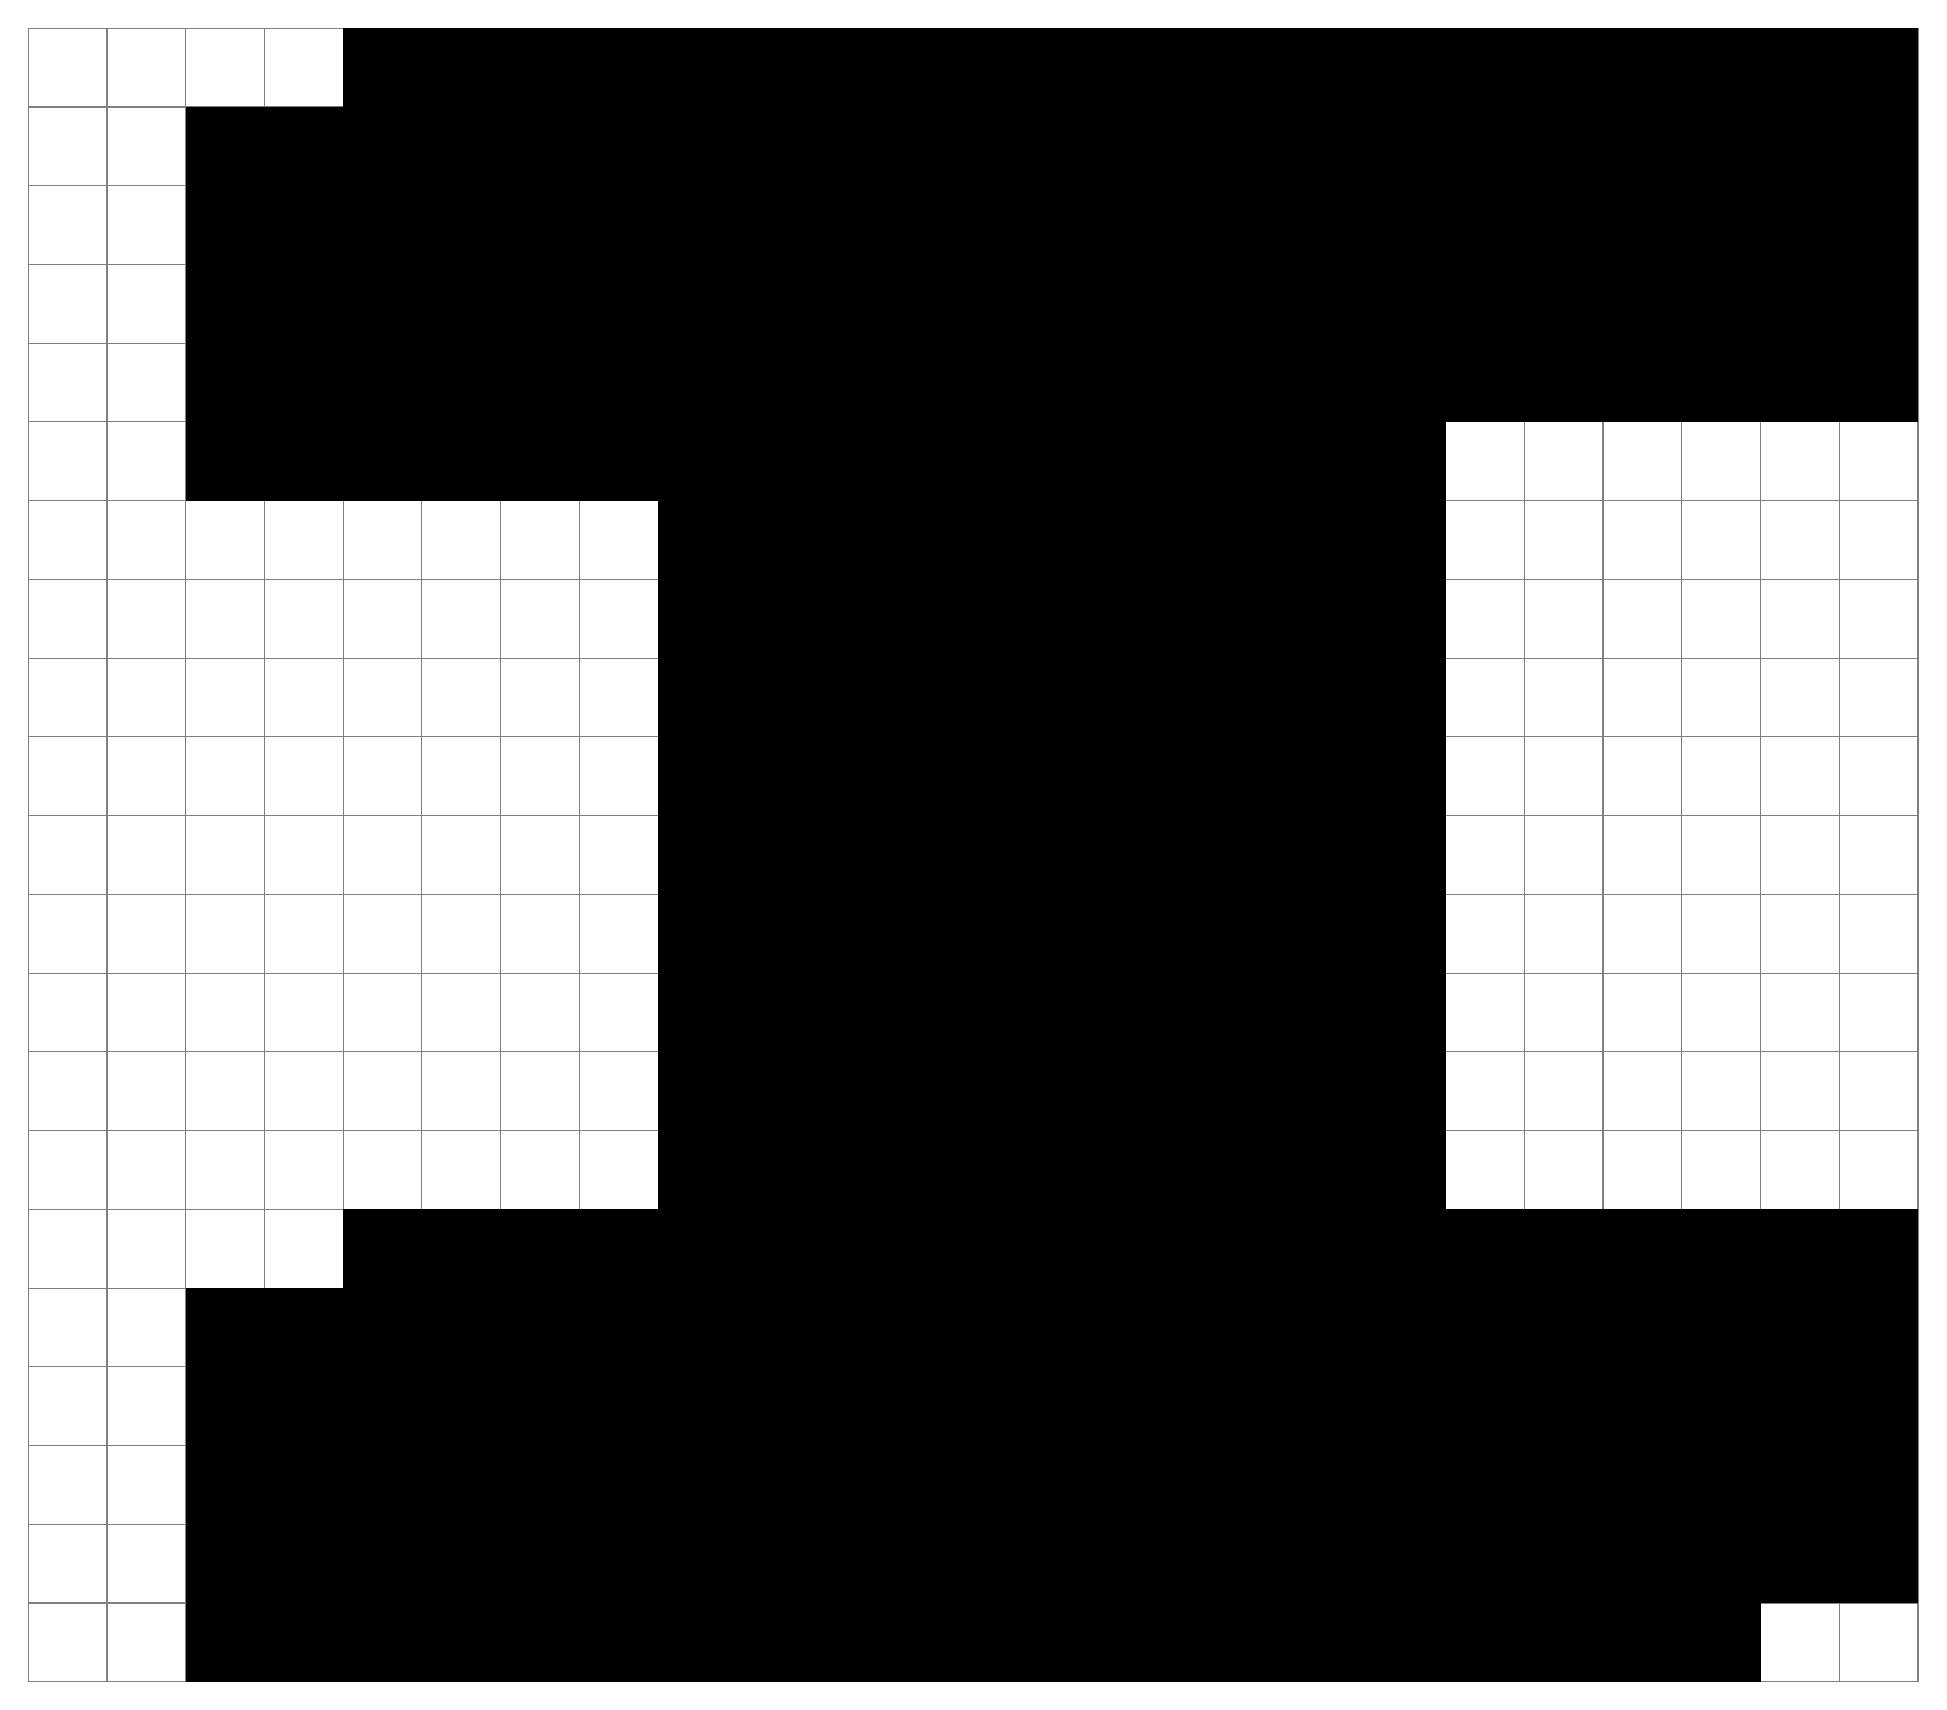
\begin{tikzpicture}

	\draw[step=1.0,gray,thin] (0,0) grid (24,21);
	\fill[\MULTICOLORTWO] (4,20) rectangle ++ (1,1);
	\fill[\MULTICOLORTWO] (5,20) rectangle ++ (1,1);
	\fill[\MULTICOLORTWO] (6,20) rectangle ++ (1,1);
	\fill[\MULTICOLORTWO] (7,20) rectangle ++ (1,1);
	\fill[\MULTICOLORTWO] (8,20) rectangle ++ (1,1);
	\fill[\MULTICOLORTWO] (9,20) rectangle ++ (1,1);
	\fill[\MULTICOLORTWO] (10,20) rectangle ++ (1,1);
	\fill[\MULTICOLORTWO] (11,20) rectangle ++ (1,1);
	\fill[\MULTICOLORTWO] (12,20) rectangle ++ (1,1);
	\fill[\MULTICOLORTWO] (13,20) rectangle ++ (1,1);
	\fill[\MULTICOLORTWO] (14,20) rectangle ++ (1,1);
	\fill[\MULTICOLORTWO] (15,20) rectangle ++ (1,1);
	\fill[\MULTICOLORTWO] (16,20) rectangle ++ (1,1);
	\fill[\MULTICOLORTWO] (17,20) rectangle ++ (1,1);
	\fill[\MULTICOLORTWO] (18,20) rectangle ++ (1,1);
	\fill[\MULTICOLORTWO] (19,20) rectangle ++ (1,1);
	\fill[\MULTICOLORTWO] (20,20) rectangle ++ (1,1);
	\fill[\MULTICOLORTWO] (21,20) rectangle ++ (1,1);
	\fill[\MULTICOLORTWO] (22,20) rectangle ++ (1,1);
	\fill[\MULTICOLORTWO] (23,20) rectangle ++ (1,1);
	\fill[\MULTICOLORONE] (2,19) rectangle ++ (1,1);
	\fill[\MULTICOLORONE] (3,19) rectangle ++ (1,1);
	\fill[\MULTICOLORTWO] (4,19) rectangle ++ (1,1);
	\fill[\MULTICOLORTWO] (5,19) rectangle ++ (1,1);
	\fill[\SPRITECOLOR] (6,19) rectangle ++ (1,1);
	\fill[\SPRITECOLOR] (7,19) rectangle ++ (1,1);
	\fill[\SPRITECOLOR] (8,19) rectangle ++ (1,1);
	\fill[\SPRITECOLOR] (9,19) rectangle ++ (1,1);
	\fill[\SPRITECOLOR] (10,19) rectangle ++ (1,1);
	\fill[\SPRITECOLOR] (11,19) rectangle ++ (1,1);
	\fill[\SPRITECOLOR] (12,19) rectangle ++ (1,1);
	\fill[\SPRITECOLOR] (13,19) rectangle ++ (1,1);
	\fill[\SPRITECOLOR] (14,19) rectangle ++ (1,1);
	\fill[\SPRITECOLOR] (15,19) rectangle ++ (1,1);
	\fill[\SPRITECOLOR] (16,19) rectangle ++ (1,1);
	\fill[\SPRITECOLOR] (17,19) rectangle ++ (1,1);
	\fill[\SPRITECOLOR] (18,19) rectangle ++ (1,1);
	\fill[\SPRITECOLOR] (19,19) rectangle ++ (1,1);
	\fill[\SPRITECOLOR] (20,19) rectangle ++ (1,1);
	\fill[\SPRITECOLOR] (21,19) rectangle ++ (1,1);
	\fill[\MULTICOLORTWO] (22,19) rectangle ++ (1,1);
	\fill[\MULTICOLORTWO] (23,19) rectangle ++ (1,1);
	\fill[\MULTICOLORONE] (2,18) rectangle ++ (1,1);
	\fill[\MULTICOLORONE] (3,18) rectangle ++ (1,1);
	\fill[\MULTICOLORTWO] (4,18) rectangle ++ (1,1);
	\fill[\MULTICOLORTWO] (5,18) rectangle ++ (1,1);
	\fill[\SPRITECOLOR] (6,18) rectangle ++ (1,1);
	\fill[\SPRITECOLOR] (7,18) rectangle ++ (1,1);
	\fill[\SPRITECOLOR] (8,18) rectangle ++ (1,1);
	\fill[\SPRITECOLOR] (9,18) rectangle ++ (1,1);
	\fill[\SPRITECOLOR] (10,18) rectangle ++ (1,1);
	\fill[\SPRITECOLOR] (11,18) rectangle ++ (1,1);
	\fill[\SPRITECOLOR] (12,18) rectangle ++ (1,1);
	\fill[\SPRITECOLOR] (13,18) rectangle ++ (1,1);
	\fill[\SPRITECOLOR] (14,18) rectangle ++ (1,1);
	\fill[\SPRITECOLOR] (15,18) rectangle ++ (1,1);
	\fill[\SPRITECOLOR] (16,18) rectangle ++ (1,1);
	\fill[\SPRITECOLOR] (17,18) rectangle ++ (1,1);
	\fill[\SPRITECOLOR] (18,18) rectangle ++ (1,1);
	\fill[\SPRITECOLOR] (19,18) rectangle ++ (1,1);
	\fill[\SPRITECOLOR] (20,18) rectangle ++ (1,1);
	\fill[\SPRITECOLOR] (21,18) rectangle ++ (1,1);
	\fill[\MULTICOLORTWO] (22,18) rectangle ++ (1,1);
	\fill[\MULTICOLORTWO] (23,18) rectangle ++ (1,1);
	\fill[\MULTICOLORONE] (2,17) rectangle ++ (1,1);
	\fill[\MULTICOLORONE] (3,17) rectangle ++ (1,1);
	\fill[\MULTICOLORTWO] (4,17) rectangle ++ (1,1);
	\fill[\MULTICOLORTWO] (5,17) rectangle ++ (1,1);
	\fill[\SPRITECOLOR] (6,17) rectangle ++ (1,1);
	\fill[\SPRITECOLOR] (7,17) rectangle ++ (1,1);
	\fill[\SPRITECOLOR] (8,17) rectangle ++ (1,1);
	\fill[\SPRITECOLOR] (9,17) rectangle ++ (1,1);
	\fill[\SPRITECOLOR] (10,17) rectangle ++ (1,1);
	\fill[\SPRITECOLOR] (11,17) rectangle ++ (1,1);
	\fill[\SPRITECOLOR] (12,17) rectangle ++ (1,1);
	\fill[\SPRITECOLOR] (13,17) rectangle ++ (1,1);
	\fill[\SPRITECOLOR] (14,17) rectangle ++ (1,1);
	\fill[\SPRITECOLOR] (15,17) rectangle ++ (1,1);
	\fill[\SPRITECOLOR] (16,17) rectangle ++ (1,1);
	\fill[\SPRITECOLOR] (17,17) rectangle ++ (1,1);
	\fill[\SPRITECOLOR] (18,17) rectangle ++ (1,1);
	\fill[\SPRITECOLOR] (19,17) rectangle ++ (1,1);
	\fill[\SPRITECOLOR] (20,17) rectangle ++ (1,1);
	\fill[\SPRITECOLOR] (21,17) rectangle ++ (1,1);
	\fill[\MULTICOLORTWO] (22,17) rectangle ++ (1,1);
	\fill[\MULTICOLORTWO] (23,17) rectangle ++ (1,1);
	\fill[\MULTICOLORONE] (2,16) rectangle ++ (1,1);
	\fill[\MULTICOLORONE] (3,16) rectangle ++ (1,1);
	\fill[\MULTICOLORTWO] (4,16) rectangle ++ (1,1);
	\fill[\MULTICOLORTWO] (5,16) rectangle ++ (1,1);
	\fill[\MULTICOLORTWO] (6,16) rectangle ++ (1,1);
	\fill[\MULTICOLORTWO] (7,16) rectangle ++ (1,1);
	\fill[\MULTICOLORTWO] (8,16) rectangle ++ (1,1);
	\fill[\MULTICOLORTWO] (9,16) rectangle ++ (1,1);
	\fill[\MULTICOLORTWO] (10,16) rectangle ++ (1,1);
	\fill[\MULTICOLORTWO] (11,16) rectangle ++ (1,1);
	\fill[\SPRITECOLOR] (12,16) rectangle ++ (1,1);
	\fill[\SPRITECOLOR] (13,16) rectangle ++ (1,1);
	\fill[\SPRITECOLOR] (14,16) rectangle ++ (1,1);
	\fill[\SPRITECOLOR] (15,16) rectangle ++ (1,1);
	\fill[\MULTICOLORTWO] (16,16) rectangle ++ (1,1);
	\fill[\MULTICOLORTWO] (17,16) rectangle ++ (1,1);
	\fill[\MULTICOLORTWO] (18,16) rectangle ++ (1,1);
	\fill[\MULTICOLORTWO] (19,16) rectangle ++ (1,1);
	\fill[\MULTICOLORTWO] (20,16) rectangle ++ (1,1);
	\fill[\MULTICOLORTWO] (21,16) rectangle ++ (1,1);
	\fill[\MULTICOLORTWO] (22,16) rectangle ++ (1,1);
	\fill[\MULTICOLORTWO] (23,16) rectangle ++ (1,1);
	\fill[\MULTICOLORONE] (2,15) rectangle ++ (1,1);
	\fill[\MULTICOLORONE] (3,15) rectangle ++ (1,1);
	\fill[\MULTICOLORONE] (4,15) rectangle ++ (1,1);
	\fill[\MULTICOLORONE] (5,15) rectangle ++ (1,1);
	\fill[\MULTICOLORONE] (6,15) rectangle ++ (1,1);
	\fill[\MULTICOLORONE] (7,15) rectangle ++ (1,1);
	\fill[\MULTICOLORONE] (8,15) rectangle ++ (1,1);
	\fill[\MULTICOLORONE] (9,15) rectangle ++ (1,1);
	\fill[\MULTICOLORTWO] (10,15) rectangle ++ (1,1);
	\fill[\MULTICOLORTWO] (11,15) rectangle ++ (1,1);
	\fill[\SPRITECOLOR] (12,15) rectangle ++ (1,1);
	\fill[\SPRITECOLOR] (13,15) rectangle ++ (1,1);
	\fill[\SPRITECOLOR] (14,15) rectangle ++ (1,1);
	\fill[\SPRITECOLOR] (15,15) rectangle ++ (1,1);
	\fill[\MULTICOLORTWO] (16,15) rectangle ++ (1,1);
	\fill[\MULTICOLORTWO] (17,15) rectangle ++ (1,1);
	\fill[\MULTICOLORONE] (8,14) rectangle ++ (1,1);
	\fill[\MULTICOLORONE] (9,14) rectangle ++ (1,1);
	\fill[\MULTICOLORTWO] (10,14) rectangle ++ (1,1);
	\fill[\MULTICOLORTWO] (11,14) rectangle ++ (1,1);
	\fill[\SPRITECOLOR] (12,14) rectangle ++ (1,1);
	\fill[\SPRITECOLOR] (13,14) rectangle ++ (1,1);
	\fill[\SPRITECOLOR] (14,14) rectangle ++ (1,1);
	\fill[\SPRITECOLOR] (15,14) rectangle ++ (1,1);
	\fill[\MULTICOLORTWO] (16,14) rectangle ++ (1,1);
	\fill[\MULTICOLORTWO] (17,14) rectangle ++ (1,1);
	\fill[\MULTICOLORONE] (8,13) rectangle ++ (1,1);
	\fill[\MULTICOLORONE] (9,13) rectangle ++ (1,1);
	\fill[\MULTICOLORTWO] (10,13) rectangle ++ (1,1);
	\fill[\MULTICOLORTWO] (11,13) rectangle ++ (1,1);
	\fill[\SPRITECOLOR] (12,13) rectangle ++ (1,1);
	\fill[\SPRITECOLOR] (13,13) rectangle ++ (1,1);
	\fill[\SPRITECOLOR] (14,13) rectangle ++ (1,1);
	\fill[\SPRITECOLOR] (15,13) rectangle ++ (1,1);
	\fill[\MULTICOLORTWO] (16,13) rectangle ++ (1,1);
	\fill[\MULTICOLORTWO] (17,13) rectangle ++ (1,1);
	\fill[\MULTICOLORONE] (8,12) rectangle ++ (1,1);
	\fill[\MULTICOLORONE] (9,12) rectangle ++ (1,1);
	\fill[\MULTICOLORTWO] (10,12) rectangle ++ (1,1);
	\fill[\MULTICOLORTWO] (11,12) rectangle ++ (1,1);
	\fill[\SPRITECOLOR] (12,12) rectangle ++ (1,1);
	\fill[\SPRITECOLOR] (13,12) rectangle ++ (1,1);
	\fill[\SPRITECOLOR] (14,12) rectangle ++ (1,1);
	\fill[\SPRITECOLOR] (15,12) rectangle ++ (1,1);
	\fill[\MULTICOLORTWO] (16,12) rectangle ++ (1,1);
	\fill[\MULTICOLORTWO] (17,12) rectangle ++ (1,1);
	\fill[\MULTICOLORONE] (8,11) rectangle ++ (1,1);
	\fill[\MULTICOLORONE] (9,11) rectangle ++ (1,1);
	\fill[\MULTICOLORTWO] (10,11) rectangle ++ (1,1);
	\fill[\MULTICOLORTWO] (11,11) rectangle ++ (1,1);
	\fill[\SPRITECOLOR] (12,11) rectangle ++ (1,1);
	\fill[\SPRITECOLOR] (13,11) rectangle ++ (1,1);
	\fill[\SPRITECOLOR] (14,11) rectangle ++ (1,1);
	\fill[\SPRITECOLOR] (15,11) rectangle ++ (1,1);
	\fill[\MULTICOLORTWO] (16,11) rectangle ++ (1,1);
	\fill[\MULTICOLORTWO] (17,11) rectangle ++ (1,1);
	\fill[\MULTICOLORONE] (8,10) rectangle ++ (1,1);
	\fill[\MULTICOLORONE] (9,10) rectangle ++ (1,1);
	\fill[\MULTICOLORTWO] (10,10) rectangle ++ (1,1);
	\fill[\MULTICOLORTWO] (11,10) rectangle ++ (1,1);
	\fill[\SPRITECOLOR] (12,10) rectangle ++ (1,1);
	\fill[\SPRITECOLOR] (13,10) rectangle ++ (1,1);
	\fill[\SPRITECOLOR] (14,10) rectangle ++ (1,1);
	\fill[\SPRITECOLOR] (15,10) rectangle ++ (1,1);
	\fill[\MULTICOLORTWO] (16,10) rectangle ++ (1,1);
	\fill[\MULTICOLORTWO] (17,10) rectangle ++ (1,1);
	\fill[\MULTICOLORONE] (8,9) rectangle ++ (1,1);
	\fill[\MULTICOLORONE] (9,9) rectangle ++ (1,1);
	\fill[\MULTICOLORTWO] (10,9) rectangle ++ (1,1);
	\fill[\MULTICOLORTWO] (11,9) rectangle ++ (1,1);
	\fill[\SPRITECOLOR] (12,9) rectangle ++ (1,1);
	\fill[\SPRITECOLOR] (13,9) rectangle ++ (1,1);
	\fill[\SPRITECOLOR] (14,9) rectangle ++ (1,1);
	\fill[\SPRITECOLOR] (15,9) rectangle ++ (1,1);
	\fill[\MULTICOLORTWO] (16,9) rectangle ++ (1,1);
	\fill[\MULTICOLORTWO] (17,9) rectangle ++ (1,1);
	\fill[\MULTICOLORONE] (8,8) rectangle ++ (1,1);
	\fill[\MULTICOLORONE] (9,8) rectangle ++ (1,1);
	\fill[\MULTICOLORTWO] (10,8) rectangle ++ (1,1);
	\fill[\MULTICOLORTWO] (11,8) rectangle ++ (1,1);
	\fill[\SPRITECOLOR] (12,8) rectangle ++ (1,1);
	\fill[\SPRITECOLOR] (13,8) rectangle ++ (1,1);
	\fill[\SPRITECOLOR] (14,8) rectangle ++ (1,1);
	\fill[\SPRITECOLOR] (15,8) rectangle ++ (1,1);
	\fill[\MULTICOLORTWO] (16,8) rectangle ++ (1,1);
	\fill[\MULTICOLORTWO] (17,8) rectangle ++ (1,1);
	\fill[\MULTICOLORONE] (8,7) rectangle ++ (1,1);
	\fill[\MULTICOLORONE] (9,7) rectangle ++ (1,1);
	\fill[\MULTICOLORTWO] (10,7) rectangle ++ (1,1);
	\fill[\MULTICOLORTWO] (11,7) rectangle ++ (1,1);
	\fill[\SPRITECOLOR] (12,7) rectangle ++ (1,1);
	\fill[\SPRITECOLOR] (13,7) rectangle ++ (1,1);
	\fill[\SPRITECOLOR] (14,7) rectangle ++ (1,1);
	\fill[\SPRITECOLOR] (15,7) rectangle ++ (1,1);
	\fill[\MULTICOLORTWO] (16,7) rectangle ++ (1,1);
	\fill[\MULTICOLORTWO] (17,7) rectangle ++ (1,1);
	\fill[\MULTICOLORONE] (8,6) rectangle ++ (1,1);
	\fill[\MULTICOLORONE] (9,6) rectangle ++ (1,1);
	\fill[\MULTICOLORTWO] (10,6) rectangle ++ (1,1);
	\fill[\MULTICOLORTWO] (11,6) rectangle ++ (1,1);
	\fill[\SPRITECOLOR] (12,6) rectangle ++ (1,1);
	\fill[\SPRITECOLOR] (13,6) rectangle ++ (1,1);
	\fill[\SPRITECOLOR] (14,6) rectangle ++ (1,1);
	\fill[\SPRITECOLOR] (15,6) rectangle ++ (1,1);
	\fill[\MULTICOLORTWO] (16,6) rectangle ++ (1,1);
	\fill[\MULTICOLORTWO] (17,6) rectangle ++ (1,1);
	\fill[\MULTICOLORTWO] (4,5) rectangle ++ (1,1);
	\fill[\MULTICOLORTWO] (5,5) rectangle ++ (1,1);
	\fill[\MULTICOLORTWO] (6,5) rectangle ++ (1,1);
	\fill[\MULTICOLORTWO] (7,5) rectangle ++ (1,1);
	\fill[\MULTICOLORTWO] (8,5) rectangle ++ (1,1);
	\fill[\MULTICOLORTWO] (9,5) rectangle ++ (1,1);
	\fill[\MULTICOLORTWO] (10,5) rectangle ++ (1,1);
	\fill[\MULTICOLORTWO] (11,5) rectangle ++ (1,1);
	\fill[\SPRITECOLOR] (12,5) rectangle ++ (1,1);
	\fill[\SPRITECOLOR] (13,5) rectangle ++ (1,1);
	\fill[\SPRITECOLOR] (14,5) rectangle ++ (1,1);
	\fill[\SPRITECOLOR] (15,5) rectangle ++ (1,1);
	\fill[\MULTICOLORTWO] (16,5) rectangle ++ (1,1);
	\fill[\MULTICOLORTWO] (17,5) rectangle ++ (1,1);
	\fill[\MULTICOLORTWO] (18,5) rectangle ++ (1,1);
	\fill[\MULTICOLORTWO] (19,5) rectangle ++ (1,1);
	\fill[\MULTICOLORTWO] (20,5) rectangle ++ (1,1);
	\fill[\MULTICOLORTWO] (21,5) rectangle ++ (1,1);
	\fill[\MULTICOLORTWO] (22,5) rectangle ++ (1,1);
	\fill[\MULTICOLORTWO] (23,5) rectangle ++ (1,1);
	\fill[\MULTICOLORONE] (2,4) rectangle ++ (1,1);
	\fill[\MULTICOLORONE] (3,4) rectangle ++ (1,1);
	\fill[\MULTICOLORTWO] (4,4) rectangle ++ (1,1);
	\fill[\MULTICOLORTWO] (5,4) rectangle ++ (1,1);
	\fill[\SPRITECOLOR] (6,4) rectangle ++ (1,1);
	\fill[\SPRITECOLOR] (7,4) rectangle ++ (1,1);
	\fill[\SPRITECOLOR] (8,4) rectangle ++ (1,1);
	\fill[\SPRITECOLOR] (9,4) rectangle ++ (1,1);
	\fill[\SPRITECOLOR] (10,4) rectangle ++ (1,1);
	\fill[\SPRITECOLOR] (11,4) rectangle ++ (1,1);
	\fill[\SPRITECOLOR] (12,4) rectangle ++ (1,1);
	\fill[\SPRITECOLOR] (13,4) rectangle ++ (1,1);
	\fill[\SPRITECOLOR] (14,4) rectangle ++ (1,1);
	\fill[\SPRITECOLOR] (15,4) rectangle ++ (1,1);
	\fill[\SPRITECOLOR] (16,4) rectangle ++ (1,1);
	\fill[\SPRITECOLOR] (17,4) rectangle ++ (1,1);
	\fill[\SPRITECOLOR] (18,4) rectangle ++ (1,1);
	\fill[\SPRITECOLOR] (19,4) rectangle ++ (1,1);
	\fill[\SPRITECOLOR] (20,4) rectangle ++ (1,1);
	\fill[\SPRITECOLOR] (21,4) rectangle ++ (1,1);
	\fill[\MULTICOLORTWO] (22,4) rectangle ++ (1,1);
	\fill[\MULTICOLORTWO] (23,4) rectangle ++ (1,1);
	\fill[\MULTICOLORONE] (2,3) rectangle ++ (1,1);
	\fill[\MULTICOLORONE] (3,3) rectangle ++ (1,1);
	\fill[\MULTICOLORTWO] (4,3) rectangle ++ (1,1);
	\fill[\MULTICOLORTWO] (5,3) rectangle ++ (1,1);
	\fill[\SPRITECOLOR] (6,3) rectangle ++ (1,1);
	\fill[\SPRITECOLOR] (7,3) rectangle ++ (1,1);
	\fill[\SPRITECOLOR] (8,3) rectangle ++ (1,1);
	\fill[\SPRITECOLOR] (9,3) rectangle ++ (1,1);
	\fill[\SPRITECOLOR] (10,3) rectangle ++ (1,1);
	\fill[\SPRITECOLOR] (11,3) rectangle ++ (1,1);
	\fill[\SPRITECOLOR] (12,3) rectangle ++ (1,1);
	\fill[\SPRITECOLOR] (13,3) rectangle ++ (1,1);
	\fill[\SPRITECOLOR] (14,3) rectangle ++ (1,1);
	\fill[\SPRITECOLOR] (15,3) rectangle ++ (1,1);
	\fill[\SPRITECOLOR] (16,3) rectangle ++ (1,1);
	\fill[\SPRITECOLOR] (17,3) rectangle ++ (1,1);
	\fill[\SPRITECOLOR] (18,3) rectangle ++ (1,1);
	\fill[\SPRITECOLOR] (19,3) rectangle ++ (1,1);
	\fill[\SPRITECOLOR] (20,3) rectangle ++ (1,1);
	\fill[\SPRITECOLOR] (21,3) rectangle ++ (1,1);
	\fill[\MULTICOLORTWO] (22,3) rectangle ++ (1,1);
	\fill[\MULTICOLORTWO] (23,3) rectangle ++ (1,1);
	\fill[\MULTICOLORONE] (2,2) rectangle ++ (1,1);
	\fill[\MULTICOLORONE] (3,2) rectangle ++ (1,1);
	\fill[\MULTICOLORTWO] (4,2) rectangle ++ (1,1);
	\fill[\MULTICOLORTWO] (5,2) rectangle ++ (1,1);
	\fill[\SPRITECOLOR] (6,2) rectangle ++ (1,1);
	\fill[\SPRITECOLOR] (7,2) rectangle ++ (1,1);
	\fill[\SPRITECOLOR] (8,2) rectangle ++ (1,1);
	\fill[\SPRITECOLOR] (9,2) rectangle ++ (1,1);
	\fill[\SPRITECOLOR] (10,2) rectangle ++ (1,1);
	\fill[\SPRITECOLOR] (11,2) rectangle ++ (1,1);
	\fill[\SPRITECOLOR] (12,2) rectangle ++ (1,1);
	\fill[\SPRITECOLOR] (13,2) rectangle ++ (1,1);
	\fill[\SPRITECOLOR] (14,2) rectangle ++ (1,1);
	\fill[\SPRITECOLOR] (15,2) rectangle ++ (1,1);
	\fill[\SPRITECOLOR] (16,2) rectangle ++ (1,1);
	\fill[\SPRITECOLOR] (17,2) rectangle ++ (1,1);
	\fill[\SPRITECOLOR] (18,2) rectangle ++ (1,1);
	\fill[\SPRITECOLOR] (19,2) rectangle ++ (1,1);
	\fill[\SPRITECOLOR] (20,2) rectangle ++ (1,1);
	\fill[\SPRITECOLOR] (21,2) rectangle ++ (1,1);
	\fill[\MULTICOLORTWO] (22,2) rectangle ++ (1,1);
	\fill[\MULTICOLORTWO] (23,2) rectangle ++ (1,1);
	\fill[\MULTICOLORONE] (2,1) rectangle ++ (1,1);
	\fill[\MULTICOLORONE] (3,1) rectangle ++ (1,1);
	\fill[\MULTICOLORTWO] (4,1) rectangle ++ (1,1);
	\fill[\MULTICOLORTWO] (5,1) rectangle ++ (1,1);
	\fill[\MULTICOLORTWO] (6,1) rectangle ++ (1,1);
	\fill[\MULTICOLORTWO] (7,1) rectangle ++ (1,1);
	\fill[\MULTICOLORTWO] (8,1) rectangle ++ (1,1);
	\fill[\MULTICOLORTWO] (9,1) rectangle ++ (1,1);
	\fill[\MULTICOLORTWO] (10,1) rectangle ++ (1,1);
	\fill[\MULTICOLORTWO] (11,1) rectangle ++ (1,1);
	\fill[\MULTICOLORTWO] (12,1) rectangle ++ (1,1);
	\fill[\MULTICOLORTWO] (13,1) rectangle ++ (1,1);
	\fill[\MULTICOLORTWO] (14,1) rectangle ++ (1,1);
	\fill[\MULTICOLORTWO] (15,1) rectangle ++ (1,1);
	\fill[\MULTICOLORTWO] (16,1) rectangle ++ (1,1);
	\fill[\MULTICOLORTWO] (17,1) rectangle ++ (1,1);
	\fill[\MULTICOLORTWO] (18,1) rectangle ++ (1,1);
	\fill[\MULTICOLORTWO] (19,1) rectangle ++ (1,1);
	\fill[\MULTICOLORTWO] (20,1) rectangle ++ (1,1);
	\fill[\MULTICOLORTWO] (21,1) rectangle ++ (1,1);
	\fill[\MULTICOLORTWO] (22,1) rectangle ++ (1,1);
	\fill[\MULTICOLORTWO] (23,1) rectangle ++ (1,1);
	\fill[\MULTICOLORONE] (2,0) rectangle ++ (1,1);
	\fill[\MULTICOLORONE] (3,0) rectangle ++ (1,1);
	\fill[\MULTICOLORONE] (4,0) rectangle ++ (1,1);
	\fill[\MULTICOLORONE] (5,0) rectangle ++ (1,1);
	\fill[\MULTICOLORONE] (6,0) rectangle ++ (1,1);
	\fill[\MULTICOLORONE] (7,0) rectangle ++ (1,1);
	\fill[\MULTICOLORONE] (8,0) rectangle ++ (1,1);
	\fill[\MULTICOLORONE] (9,0) rectangle ++ (1,1);
	\fill[\MULTICOLORONE] (10,0) rectangle ++ (1,1);
	\fill[\MULTICOLORONE] (11,0) rectangle ++ (1,1);
	\fill[\MULTICOLORONE] (12,0) rectangle ++ (1,1);
	\fill[\MULTICOLORONE] (13,0) rectangle ++ (1,1);
	\fill[\MULTICOLORONE] (14,0) rectangle ++ (1,1);
	\fill[\MULTICOLORONE] (15,0) rectangle ++ (1,1);
	\fill[\MULTICOLORONE] (16,0) rectangle ++ (1,1);
	\fill[\MULTICOLORONE] (17,0) rectangle ++ (1,1);
	\fill[\MULTICOLORONE] (18,0) rectangle ++ (1,1);
	\fill[\MULTICOLORONE] (19,0) rectangle ++ (1,1);
	\fill[\MULTICOLORONE] (20,0) rectangle ++ (1,1);
	\fill[\MULTICOLORONE] (21,0) rectangle ++ (1,1);

      \end{tikzpicture}
    \end{adjustbox}
  }\caption{BIG\_I}
\end{figure}

	\end{subfigure}
} &
\makecell[l]{
	\begin{subfigure}{0.3\textwidth}
    \def\MULTICOLORONE{gray}
    \def\MULTICOLORTWO{black}
    \def\SPRITECOLOR{gray}
		
\begin{figure}[H]
  {
    \setlength{\tabcolsep}{3.0pt}
    \setlength\cmidrulewidth{\heavyrulewidth} % Make cmidrule = 
    \begin{adjustbox}{width=3cm,center}
      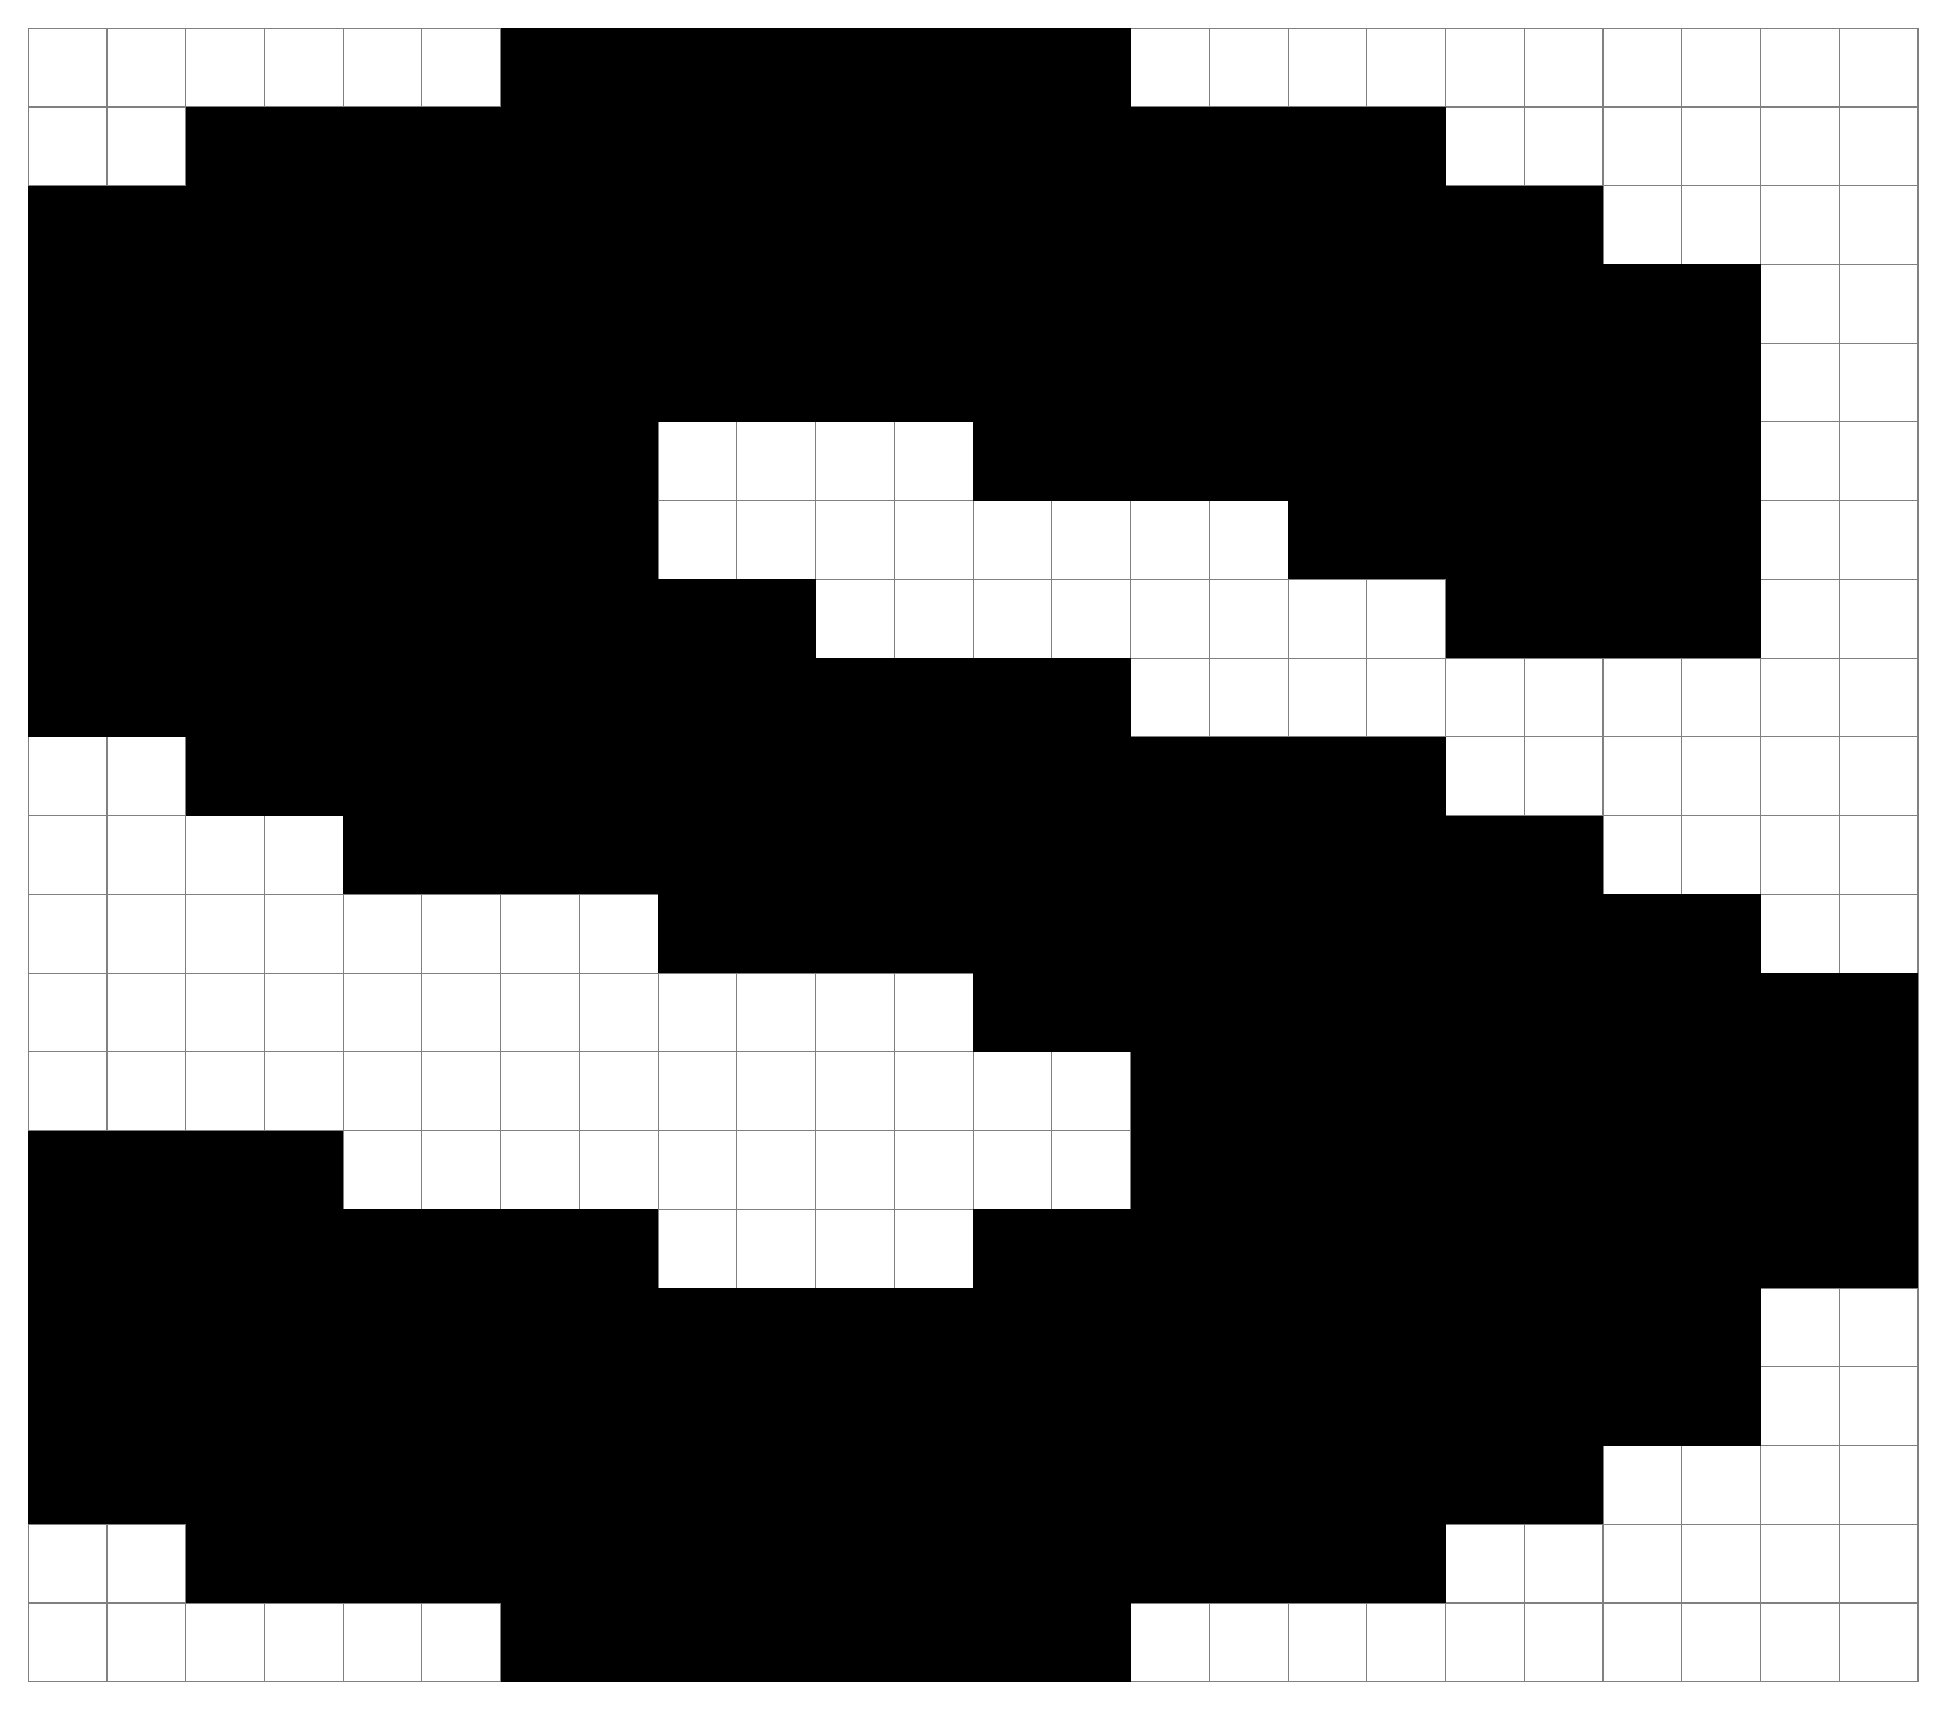
\begin{tikzpicture}

	\draw[step=1.0,gray,thin] (0,0) grid (24,21);
	\fill[\MULTICOLORONE] (6,20) rectangle ++ (1,1);
	\fill[\MULTICOLORONE] (7,20) rectangle ++ (1,1);
	\fill[\MULTICOLORTWO] (8,20) rectangle ++ (1,1);
	\fill[\MULTICOLORTWO] (9,20) rectangle ++ (1,1);
	\fill[\MULTICOLORTWO] (10,20) rectangle ++ (1,1);
	\fill[\MULTICOLORTWO] (11,20) rectangle ++ (1,1);
	\fill[\MULTICOLORTWO] (12,20) rectangle ++ (1,1);
	\fill[\MULTICOLORTWO] (13,20) rectangle ++ (1,1);
	\fill[\MULTICOLORONE] (2,19) rectangle ++ (1,1);
	\fill[\MULTICOLORONE] (3,19) rectangle ++ (1,1);
	\fill[\MULTICOLORTWO] (4,19) rectangle ++ (1,1);
	\fill[\MULTICOLORTWO] (5,19) rectangle ++ (1,1);
	\fill[\MULTICOLORTWO] (6,19) rectangle ++ (1,1);
	\fill[\MULTICOLORTWO] (7,19) rectangle ++ (1,1);
	\fill[\SPRITECOLOR] (8,19) rectangle ++ (1,1);
	\fill[\SPRITECOLOR] (9,19) rectangle ++ (1,1);
	\fill[\SPRITECOLOR] (10,19) rectangle ++ (1,1);
	\fill[\SPRITECOLOR] (11,19) rectangle ++ (1,1);
	\fill[\SPRITECOLOR] (12,19) rectangle ++ (1,1);
	\fill[\SPRITECOLOR] (13,19) rectangle ++ (1,1);
	\fill[\MULTICOLORTWO] (14,19) rectangle ++ (1,1);
	\fill[\MULTICOLORTWO] (15,19) rectangle ++ (1,1);
	\fill[\MULTICOLORTWO] (16,19) rectangle ++ (1,1);
	\fill[\MULTICOLORTWO] (17,19) rectangle ++ (1,1);
	\fill[\MULTICOLORONE] (0,18) rectangle ++ (1,1);
	\fill[\MULTICOLORONE] (1,18) rectangle ++ (1,1);
	\fill[\MULTICOLORTWO] (2,18) rectangle ++ (1,1);
	\fill[\MULTICOLORTWO] (3,18) rectangle ++ (1,1);
	\fill[\SPRITECOLOR] (4,18) rectangle ++ (1,1);
	\fill[\SPRITECOLOR] (5,18) rectangle ++ (1,1);
	\fill[\SPRITECOLOR] (6,18) rectangle ++ (1,1);
	\fill[\SPRITECOLOR] (7,18) rectangle ++ (1,1);
	\fill[\SPRITECOLOR] (8,18) rectangle ++ (1,1);
	\fill[\SPRITECOLOR] (9,18) rectangle ++ (1,1);
	\fill[\SPRITECOLOR] (10,18) rectangle ++ (1,1);
	\fill[\SPRITECOLOR] (11,18) rectangle ++ (1,1);
	\fill[\SPRITECOLOR] (12,18) rectangle ++ (1,1);
	\fill[\SPRITECOLOR] (13,18) rectangle ++ (1,1);
	\fill[\SPRITECOLOR] (14,18) rectangle ++ (1,1);
	\fill[\SPRITECOLOR] (15,18) rectangle ++ (1,1);
	\fill[\SPRITECOLOR] (16,18) rectangle ++ (1,1);
	\fill[\SPRITECOLOR] (17,18) rectangle ++ (1,1);
	\fill[\MULTICOLORTWO] (18,18) rectangle ++ (1,1);
	\fill[\MULTICOLORTWO] (19,18) rectangle ++ (1,1);
	\fill[\MULTICOLORTWO] (0,17) rectangle ++ (1,1);
	\fill[\MULTICOLORTWO] (1,17) rectangle ++ (1,1);
	\fill[\SPRITECOLOR] (2,17) rectangle ++ (1,1);
	\fill[\SPRITECOLOR] (3,17) rectangle ++ (1,1);
	\fill[\SPRITECOLOR] (4,17) rectangle ++ (1,1);
	\fill[\SPRITECOLOR] (5,17) rectangle ++ (1,1);
	\fill[\SPRITECOLOR] (6,17) rectangle ++ (1,1);
	\fill[\SPRITECOLOR] (7,17) rectangle ++ (1,1);
	\fill[\SPRITECOLOR] (8,17) rectangle ++ (1,1);
	\fill[\SPRITECOLOR] (9,17) rectangle ++ (1,1);
	\fill[\SPRITECOLOR] (10,17) rectangle ++ (1,1);
	\fill[\SPRITECOLOR] (11,17) rectangle ++ (1,1);
	\fill[\SPRITECOLOR] (12,17) rectangle ++ (1,1);
	\fill[\SPRITECOLOR] (13,17) rectangle ++ (1,1);
	\fill[\SPRITECOLOR] (14,17) rectangle ++ (1,1);
	\fill[\SPRITECOLOR] (15,17) rectangle ++ (1,1);
	\fill[\SPRITECOLOR] (16,17) rectangle ++ (1,1);
	\fill[\SPRITECOLOR] (17,17) rectangle ++ (1,1);
	\fill[\SPRITECOLOR] (18,17) rectangle ++ (1,1);
	\fill[\SPRITECOLOR] (19,17) rectangle ++ (1,1);
	\fill[\MULTICOLORTWO] (20,17) rectangle ++ (1,1);
	\fill[\MULTICOLORTWO] (21,17) rectangle ++ (1,1);
	\fill[\MULTICOLORTWO] (0,16) rectangle ++ (1,1);
	\fill[\MULTICOLORTWO] (1,16) rectangle ++ (1,1);
	\fill[\SPRITECOLOR] (2,16) rectangle ++ (1,1);
	\fill[\SPRITECOLOR] (3,16) rectangle ++ (1,1);
	\fill[\SPRITECOLOR] (4,16) rectangle ++ (1,1);
	\fill[\SPRITECOLOR] (5,16) rectangle ++ (1,1);
	\fill[\SPRITECOLOR] (6,16) rectangle ++ (1,1);
	\fill[\SPRITECOLOR] (7,16) rectangle ++ (1,1);
	\fill[\MULTICOLORTWO] (8,16) rectangle ++ (1,1);
	\fill[\MULTICOLORTWO] (9,16) rectangle ++ (1,1);
	\fill[\MULTICOLORTWO] (10,16) rectangle ++ (1,1);
	\fill[\MULTICOLORTWO] (11,16) rectangle ++ (1,1);
	\fill[\MULTICOLORTWO] (12,16) rectangle ++ (1,1);
	\fill[\MULTICOLORTWO] (13,16) rectangle ++ (1,1);
	\fill[\SPRITECOLOR] (14,16) rectangle ++ (1,1);
	\fill[\SPRITECOLOR] (15,16) rectangle ++ (1,1);
	\fill[\SPRITECOLOR] (16,16) rectangle ++ (1,1);
	\fill[\SPRITECOLOR] (17,16) rectangle ++ (1,1);
	\fill[\SPRITECOLOR] (18,16) rectangle ++ (1,1);
	\fill[\SPRITECOLOR] (19,16) rectangle ++ (1,1);
	\fill[\MULTICOLORTWO] (20,16) rectangle ++ (1,1);
	\fill[\MULTICOLORTWO] (21,16) rectangle ++ (1,1);
	\fill[\MULTICOLORTWO] (0,15) rectangle ++ (1,1);
	\fill[\MULTICOLORTWO] (1,15) rectangle ++ (1,1);
	\fill[\SPRITECOLOR] (2,15) rectangle ++ (1,1);
	\fill[\SPRITECOLOR] (3,15) rectangle ++ (1,1);
	\fill[\SPRITECOLOR] (4,15) rectangle ++ (1,1);
	\fill[\SPRITECOLOR] (5,15) rectangle ++ (1,1);
	\fill[\MULTICOLORTWO] (6,15) rectangle ++ (1,1);
	\fill[\MULTICOLORTWO] (7,15) rectangle ++ (1,1);
	\fill[\MULTICOLORONE] (12,15) rectangle ++ (1,1);
	\fill[\MULTICOLORONE] (13,15) rectangle ++ (1,1);
	\fill[\MULTICOLORTWO] (14,15) rectangle ++ (1,1);
	\fill[\MULTICOLORTWO] (15,15) rectangle ++ (1,1);
	\fill[\MULTICOLORTWO] (16,15) rectangle ++ (1,1);
	\fill[\MULTICOLORTWO] (17,15) rectangle ++ (1,1);
	\fill[\SPRITECOLOR] (18,15) rectangle ++ (1,1);
	\fill[\SPRITECOLOR] (19,15) rectangle ++ (1,1);
	\fill[\MULTICOLORTWO] (20,15) rectangle ++ (1,1);
	\fill[\MULTICOLORTWO] (21,15) rectangle ++ (1,1);
	\fill[\MULTICOLORTWO] (0,14) rectangle ++ (1,1);
	\fill[\MULTICOLORTWO] (1,14) rectangle ++ (1,1);
	\fill[\SPRITECOLOR] (2,14) rectangle ++ (1,1);
	\fill[\SPRITECOLOR] (3,14) rectangle ++ (1,1);
	\fill[\SPRITECOLOR] (4,14) rectangle ++ (1,1);
	\fill[\SPRITECOLOR] (5,14) rectangle ++ (1,1);
	\fill[\MULTICOLORTWO] (6,14) rectangle ++ (1,1);
	\fill[\MULTICOLORTWO] (7,14) rectangle ++ (1,1);
	\fill[\MULTICOLORONE] (16,14) rectangle ++ (1,1);
	\fill[\MULTICOLORONE] (17,14) rectangle ++ (1,1);
	\fill[\MULTICOLORTWO] (18,14) rectangle ++ (1,1);
	\fill[\MULTICOLORTWO] (19,14) rectangle ++ (1,1);
	\fill[\MULTICOLORTWO] (20,14) rectangle ++ (1,1);
	\fill[\MULTICOLORTWO] (21,14) rectangle ++ (1,1);
	\fill[\MULTICOLORTWO] (0,13) rectangle ++ (1,1);
	\fill[\MULTICOLORTWO] (1,13) rectangle ++ (1,1);
	\fill[\SPRITECOLOR] (2,13) rectangle ++ (1,1);
	\fill[\SPRITECOLOR] (3,13) rectangle ++ (1,1);
	\fill[\SPRITECOLOR] (4,13) rectangle ++ (1,1);
	\fill[\SPRITECOLOR] (5,13) rectangle ++ (1,1);
	\fill[\SPRITECOLOR] (6,13) rectangle ++ (1,1);
	\fill[\SPRITECOLOR] (7,13) rectangle ++ (1,1);
	\fill[\MULTICOLORTWO] (8,13) rectangle ++ (1,1);
	\fill[\MULTICOLORTWO] (9,13) rectangle ++ (1,1);
	\fill[\MULTICOLORONE] (18,13) rectangle ++ (1,1);
	\fill[\MULTICOLORONE] (19,13) rectangle ++ (1,1);
	\fill[\MULTICOLORTWO] (20,13) rectangle ++ (1,1);
	\fill[\MULTICOLORTWO] (21,13) rectangle ++ (1,1);
	\fill[\MULTICOLORONE] (0,12) rectangle ++ (1,1);
	\fill[\MULTICOLORONE] (1,12) rectangle ++ (1,1);
	\fill[\MULTICOLORTWO] (2,12) rectangle ++ (1,1);
	\fill[\MULTICOLORTWO] (3,12) rectangle ++ (1,1);
	\fill[\SPRITECOLOR] (4,12) rectangle ++ (1,1);
	\fill[\SPRITECOLOR] (5,12) rectangle ++ (1,1);
	\fill[\SPRITECOLOR] (6,12) rectangle ++ (1,1);
	\fill[\SPRITECOLOR] (7,12) rectangle ++ (1,1);
	\fill[\SPRITECOLOR] (8,12) rectangle ++ (1,1);
	\fill[\SPRITECOLOR] (9,12) rectangle ++ (1,1);
	\fill[\MULTICOLORTWO] (10,12) rectangle ++ (1,1);
	\fill[\MULTICOLORTWO] (11,12) rectangle ++ (1,1);
	\fill[\MULTICOLORTWO] (12,12) rectangle ++ (1,1);
	\fill[\MULTICOLORTWO] (13,12) rectangle ++ (1,1);
	\fill[\MULTICOLORONE] (2,11) rectangle ++ (1,1);
	\fill[\MULTICOLORONE] (3,11) rectangle ++ (1,1);
	\fill[\MULTICOLORTWO] (4,11) rectangle ++ (1,1);
	\fill[\MULTICOLORTWO] (5,11) rectangle ++ (1,1);
	\fill[\SPRITECOLOR] (6,11) rectangle ++ (1,1);
	\fill[\SPRITECOLOR] (7,11) rectangle ++ (1,1);
	\fill[\SPRITECOLOR] (8,11) rectangle ++ (1,1);
	\fill[\SPRITECOLOR] (9,11) rectangle ++ (1,1);
	\fill[\SPRITECOLOR] (10,11) rectangle ++ (1,1);
	\fill[\SPRITECOLOR] (11,11) rectangle ++ (1,1);
	\fill[\SPRITECOLOR] (12,11) rectangle ++ (1,1);
	\fill[\SPRITECOLOR] (13,11) rectangle ++ (1,1);
	\fill[\MULTICOLORTWO] (14,11) rectangle ++ (1,1);
	\fill[\MULTICOLORTWO] (15,11) rectangle ++ (1,1);
	\fill[\MULTICOLORTWO] (16,11) rectangle ++ (1,1);
	\fill[\MULTICOLORTWO] (17,11) rectangle ++ (1,1);
	\fill[\MULTICOLORONE] (4,10) rectangle ++ (1,1);
	\fill[\MULTICOLORONE] (5,10) rectangle ++ (1,1);
	\fill[\MULTICOLORTWO] (6,10) rectangle ++ (1,1);
	\fill[\MULTICOLORTWO] (7,10) rectangle ++ (1,1);
	\fill[\MULTICOLORTWO] (8,10) rectangle ++ (1,1);
	\fill[\MULTICOLORTWO] (9,10) rectangle ++ (1,1);
	\fill[\SPRITECOLOR] (10,10) rectangle ++ (1,1);
	\fill[\SPRITECOLOR] (11,10) rectangle ++ (1,1);
	\fill[\SPRITECOLOR] (12,10) rectangle ++ (1,1);
	\fill[\SPRITECOLOR] (13,10) rectangle ++ (1,1);
	\fill[\SPRITECOLOR] (14,10) rectangle ++ (1,1);
	\fill[\SPRITECOLOR] (15,10) rectangle ++ (1,1);
	\fill[\SPRITECOLOR] (16,10) rectangle ++ (1,1);
	\fill[\SPRITECOLOR] (17,10) rectangle ++ (1,1);
	\fill[\MULTICOLORTWO] (18,10) rectangle ++ (1,1);
	\fill[\MULTICOLORTWO] (19,10) rectangle ++ (1,1);
	\fill[\MULTICOLORONE] (8,9) rectangle ++ (1,1);
	\fill[\MULTICOLORONE] (9,9) rectangle ++ (1,1);
	\fill[\MULTICOLORTWO] (10,9) rectangle ++ (1,1);
	\fill[\MULTICOLORTWO] (11,9) rectangle ++ (1,1);
	\fill[\MULTICOLORTWO] (12,9) rectangle ++ (1,1);
	\fill[\MULTICOLORTWO] (13,9) rectangle ++ (1,1);
	\fill[\SPRITECOLOR] (14,9) rectangle ++ (1,1);
	\fill[\SPRITECOLOR] (15,9) rectangle ++ (1,1);
	\fill[\SPRITECOLOR] (16,9) rectangle ++ (1,1);
	\fill[\SPRITECOLOR] (17,9) rectangle ++ (1,1);
	\fill[\SPRITECOLOR] (18,9) rectangle ++ (1,1);
	\fill[\SPRITECOLOR] (19,9) rectangle ++ (1,1);
	\fill[\MULTICOLORTWO] (20,9) rectangle ++ (1,1);
	\fill[\MULTICOLORTWO] (21,9) rectangle ++ (1,1);
	\fill[\MULTICOLORONE] (12,8) rectangle ++ (1,1);
	\fill[\MULTICOLORONE] (13,8) rectangle ++ (1,1);
	\fill[\MULTICOLORTWO] (14,8) rectangle ++ (1,1);
	\fill[\MULTICOLORTWO] (15,8) rectangle ++ (1,1);
	\fill[\SPRITECOLOR] (16,8) rectangle ++ (1,1);
	\fill[\SPRITECOLOR] (17,8) rectangle ++ (1,1);
	\fill[\SPRITECOLOR] (18,8) rectangle ++ (1,1);
	\fill[\SPRITECOLOR] (19,8) rectangle ++ (1,1);
	\fill[\SPRITECOLOR] (20,8) rectangle ++ (1,1);
	\fill[\SPRITECOLOR] (21,8) rectangle ++ (1,1);
	\fill[\MULTICOLORTWO] (22,8) rectangle ++ (1,1);
	\fill[\MULTICOLORTWO] (23,8) rectangle ++ (1,1);
	\fill[\MULTICOLORONE] (14,7) rectangle ++ (1,1);
	\fill[\MULTICOLORONE] (15,7) rectangle ++ (1,1);
	\fill[\MULTICOLORTWO] (16,7) rectangle ++ (1,1);
	\fill[\MULTICOLORTWO] (17,7) rectangle ++ (1,1);
	\fill[\SPRITECOLOR] (18,7) rectangle ++ (1,1);
	\fill[\SPRITECOLOR] (19,7) rectangle ++ (1,1);
	\fill[\SPRITECOLOR] (20,7) rectangle ++ (1,1);
	\fill[\SPRITECOLOR] (21,7) rectangle ++ (1,1);
	\fill[\MULTICOLORTWO] (22,7) rectangle ++ (1,1);
	\fill[\MULTICOLORTWO] (23,7) rectangle ++ (1,1);
	\fill[\MULTICOLORTWO] (0,6) rectangle ++ (1,1);
	\fill[\MULTICOLORTWO] (1,6) rectangle ++ (1,1);
	\fill[\MULTICOLORTWO] (2,6) rectangle ++ (1,1);
	\fill[\MULTICOLORTWO] (3,6) rectangle ++ (1,1);
	\fill[\MULTICOLORONE] (14,6) rectangle ++ (1,1);
	\fill[\MULTICOLORONE] (15,6) rectangle ++ (1,1);
	\fill[\MULTICOLORTWO] (16,6) rectangle ++ (1,1);
	\fill[\MULTICOLORTWO] (17,6) rectangle ++ (1,1);
	\fill[\SPRITECOLOR] (18,6) rectangle ++ (1,1);
	\fill[\SPRITECOLOR] (19,6) rectangle ++ (1,1);
	\fill[\SPRITECOLOR] (20,6) rectangle ++ (1,1);
	\fill[\SPRITECOLOR] (21,6) rectangle ++ (1,1);
	\fill[\MULTICOLORTWO] (22,6) rectangle ++ (1,1);
	\fill[\MULTICOLORTWO] (23,6) rectangle ++ (1,1);
	\fill[\MULTICOLORTWO] (0,5) rectangle ++ (1,1);
	\fill[\MULTICOLORTWO] (1,5) rectangle ++ (1,1);
	\fill[\SPRITECOLOR] (2,5) rectangle ++ (1,1);
	\fill[\SPRITECOLOR] (3,5) rectangle ++ (1,1);
	\fill[\MULTICOLORTWO] (4,5) rectangle ++ (1,1);
	\fill[\MULTICOLORTWO] (5,5) rectangle ++ (1,1);
	\fill[\MULTICOLORTWO] (6,5) rectangle ++ (1,1);
	\fill[\MULTICOLORTWO] (7,5) rectangle ++ (1,1);
	\fill[\MULTICOLORONE] (12,5) rectangle ++ (1,1);
	\fill[\MULTICOLORONE] (13,5) rectangle ++ (1,1);
	\fill[\MULTICOLORTWO] (14,5) rectangle ++ (1,1);
	\fill[\MULTICOLORTWO] (15,5) rectangle ++ (1,1);
	\fill[\SPRITECOLOR] (16,5) rectangle ++ (1,1);
	\fill[\SPRITECOLOR] (17,5) rectangle ++ (1,1);
	\fill[\SPRITECOLOR] (18,5) rectangle ++ (1,1);
	\fill[\SPRITECOLOR] (19,5) rectangle ++ (1,1);
	\fill[\SPRITECOLOR] (20,5) rectangle ++ (1,1);
	\fill[\SPRITECOLOR] (21,5) rectangle ++ (1,1);
	\fill[\MULTICOLORTWO] (22,5) rectangle ++ (1,1);
	\fill[\MULTICOLORTWO] (23,5) rectangle ++ (1,1);
	\fill[\MULTICOLORTWO] (0,4) rectangle ++ (1,1);
	\fill[\MULTICOLORTWO] (1,4) rectangle ++ (1,1);
	\fill[\SPRITECOLOR] (2,4) rectangle ++ (1,1);
	\fill[\SPRITECOLOR] (3,4) rectangle ++ (1,1);
	\fill[\SPRITECOLOR] (4,4) rectangle ++ (1,1);
	\fill[\SPRITECOLOR] (5,4) rectangle ++ (1,1);
	\fill[\SPRITECOLOR] (6,4) rectangle ++ (1,1);
	\fill[\SPRITECOLOR] (7,4) rectangle ++ (1,1);
	\fill[\MULTICOLORTWO] (8,4) rectangle ++ (1,1);
	\fill[\MULTICOLORTWO] (9,4) rectangle ++ (1,1);
	\fill[\MULTICOLORTWO] (10,4) rectangle ++ (1,1);
	\fill[\MULTICOLORTWO] (11,4) rectangle ++ (1,1);
	\fill[\MULTICOLORTWO] (12,4) rectangle ++ (1,1);
	\fill[\MULTICOLORTWO] (13,4) rectangle ++ (1,1);
	\fill[\SPRITECOLOR] (14,4) rectangle ++ (1,1);
	\fill[\SPRITECOLOR] (15,4) rectangle ++ (1,1);
	\fill[\SPRITECOLOR] (16,4) rectangle ++ (1,1);
	\fill[\SPRITECOLOR] (17,4) rectangle ++ (1,1);
	\fill[\SPRITECOLOR] (18,4) rectangle ++ (1,1);
	\fill[\SPRITECOLOR] (19,4) rectangle ++ (1,1);
	\fill[\MULTICOLORTWO] (20,4) rectangle ++ (1,1);
	\fill[\MULTICOLORTWO] (21,4) rectangle ++ (1,1);
	\fill[\MULTICOLORTWO] (0,3) rectangle ++ (1,1);
	\fill[\MULTICOLORTWO] (1,3) rectangle ++ (1,1);
	\fill[\SPRITECOLOR] (2,3) rectangle ++ (1,1);
	\fill[\SPRITECOLOR] (3,3) rectangle ++ (1,1);
	\fill[\SPRITECOLOR] (4,3) rectangle ++ (1,1);
	\fill[\SPRITECOLOR] (5,3) rectangle ++ (1,1);
	\fill[\SPRITECOLOR] (6,3) rectangle ++ (1,1);
	\fill[\SPRITECOLOR] (7,3) rectangle ++ (1,1);
	\fill[\SPRITECOLOR] (8,3) rectangle ++ (1,1);
	\fill[\SPRITECOLOR] (9,3) rectangle ++ (1,1);
	\fill[\SPRITECOLOR] (10,3) rectangle ++ (1,1);
	\fill[\SPRITECOLOR] (11,3) rectangle ++ (1,1);
	\fill[\SPRITECOLOR] (12,3) rectangle ++ (1,1);
	\fill[\SPRITECOLOR] (13,3) rectangle ++ (1,1);
	\fill[\SPRITECOLOR] (14,3) rectangle ++ (1,1);
	\fill[\SPRITECOLOR] (15,3) rectangle ++ (1,1);
	\fill[\SPRITECOLOR] (16,3) rectangle ++ (1,1);
	\fill[\SPRITECOLOR] (17,3) rectangle ++ (1,1);
	\fill[\SPRITECOLOR] (18,3) rectangle ++ (1,1);
	\fill[\SPRITECOLOR] (19,3) rectangle ++ (1,1);
	\fill[\MULTICOLORTWO] (20,3) rectangle ++ (1,1);
	\fill[\MULTICOLORTWO] (21,3) rectangle ++ (1,1);
	\fill[\MULTICOLORTWO] (0,2) rectangle ++ (1,1);
	\fill[\MULTICOLORTWO] (1,2) rectangle ++ (1,1);
	\fill[\MULTICOLORTWO] (2,2) rectangle ++ (1,1);
	\fill[\MULTICOLORTWO] (3,2) rectangle ++ (1,1);
	\fill[\SPRITECOLOR] (4,2) rectangle ++ (1,1);
	\fill[\SPRITECOLOR] (5,2) rectangle ++ (1,1);
	\fill[\SPRITECOLOR] (6,2) rectangle ++ (1,1);
	\fill[\SPRITECOLOR] (7,2) rectangle ++ (1,1);
	\fill[\SPRITECOLOR] (8,2) rectangle ++ (1,1);
	\fill[\SPRITECOLOR] (9,2) rectangle ++ (1,1);
	\fill[\SPRITECOLOR] (10,2) rectangle ++ (1,1);
	\fill[\SPRITECOLOR] (11,2) rectangle ++ (1,1);
	\fill[\SPRITECOLOR] (12,2) rectangle ++ (1,1);
	\fill[\SPRITECOLOR] (13,2) rectangle ++ (1,1);
	\fill[\SPRITECOLOR] (14,2) rectangle ++ (1,1);
	\fill[\SPRITECOLOR] (15,2) rectangle ++ (1,1);
	\fill[\SPRITECOLOR] (16,2) rectangle ++ (1,1);
	\fill[\SPRITECOLOR] (17,2) rectangle ++ (1,1);
	\fill[\MULTICOLORTWO] (18,2) rectangle ++ (1,1);
	\fill[\MULTICOLORTWO] (19,2) rectangle ++ (1,1);
	\fill[\MULTICOLORONE] (2,1) rectangle ++ (1,1);
	\fill[\MULTICOLORONE] (3,1) rectangle ++ (1,1);
	\fill[\MULTICOLORTWO] (4,1) rectangle ++ (1,1);
	\fill[\MULTICOLORTWO] (5,1) rectangle ++ (1,1);
	\fill[\MULTICOLORTWO] (6,1) rectangle ++ (1,1);
	\fill[\MULTICOLORTWO] (7,1) rectangle ++ (1,1);
	\fill[\SPRITECOLOR] (8,1) rectangle ++ (1,1);
	\fill[\SPRITECOLOR] (9,1) rectangle ++ (1,1);
	\fill[\SPRITECOLOR] (10,1) rectangle ++ (1,1);
	\fill[\SPRITECOLOR] (11,1) rectangle ++ (1,1);
	\fill[\SPRITECOLOR] (12,1) rectangle ++ (1,1);
	\fill[\SPRITECOLOR] (13,1) rectangle ++ (1,1);
	\fill[\MULTICOLORTWO] (14,1) rectangle ++ (1,1);
	\fill[\MULTICOLORTWO] (15,1) rectangle ++ (1,1);
	\fill[\MULTICOLORTWO] (16,1) rectangle ++ (1,1);
	\fill[\MULTICOLORTWO] (17,1) rectangle ++ (1,1);
	\fill[\MULTICOLORONE] (6,0) rectangle ++ (1,1);
	\fill[\MULTICOLORONE] (7,0) rectangle ++ (1,1);
	\fill[\MULTICOLORTWO] (8,0) rectangle ++ (1,1);
	\fill[\MULTICOLORTWO] (9,0) rectangle ++ (1,1);
	\fill[\MULTICOLORTWO] (10,0) rectangle ++ (1,1);
	\fill[\MULTICOLORTWO] (11,0) rectangle ++ (1,1);
	\fill[\MULTICOLORTWO] (12,0) rectangle ++ (1,1);
	\fill[\MULTICOLORTWO] (13,0) rectangle ++ (1,1);

      \end{tikzpicture}
    \end{adjustbox}
  }\caption{IG\_S}
\end{figure}

	\end{subfigure}
} &
\makecell[l]{
	\begin{subfigure}{0.3\textwidth}
    \def\MULTICOLORONE{gray}
    \def\MULTICOLORTWO{gray}
    \def\SPRITECOLOR{gray}
		
\begin{figure}[H]
  {
    \setlength{\tabcolsep}{3.0pt}
    \setlength\cmidrulewidth{\heavyrulewidth} % Make cmidrule = 
    \begin{adjustbox}{width=3cm,center}
      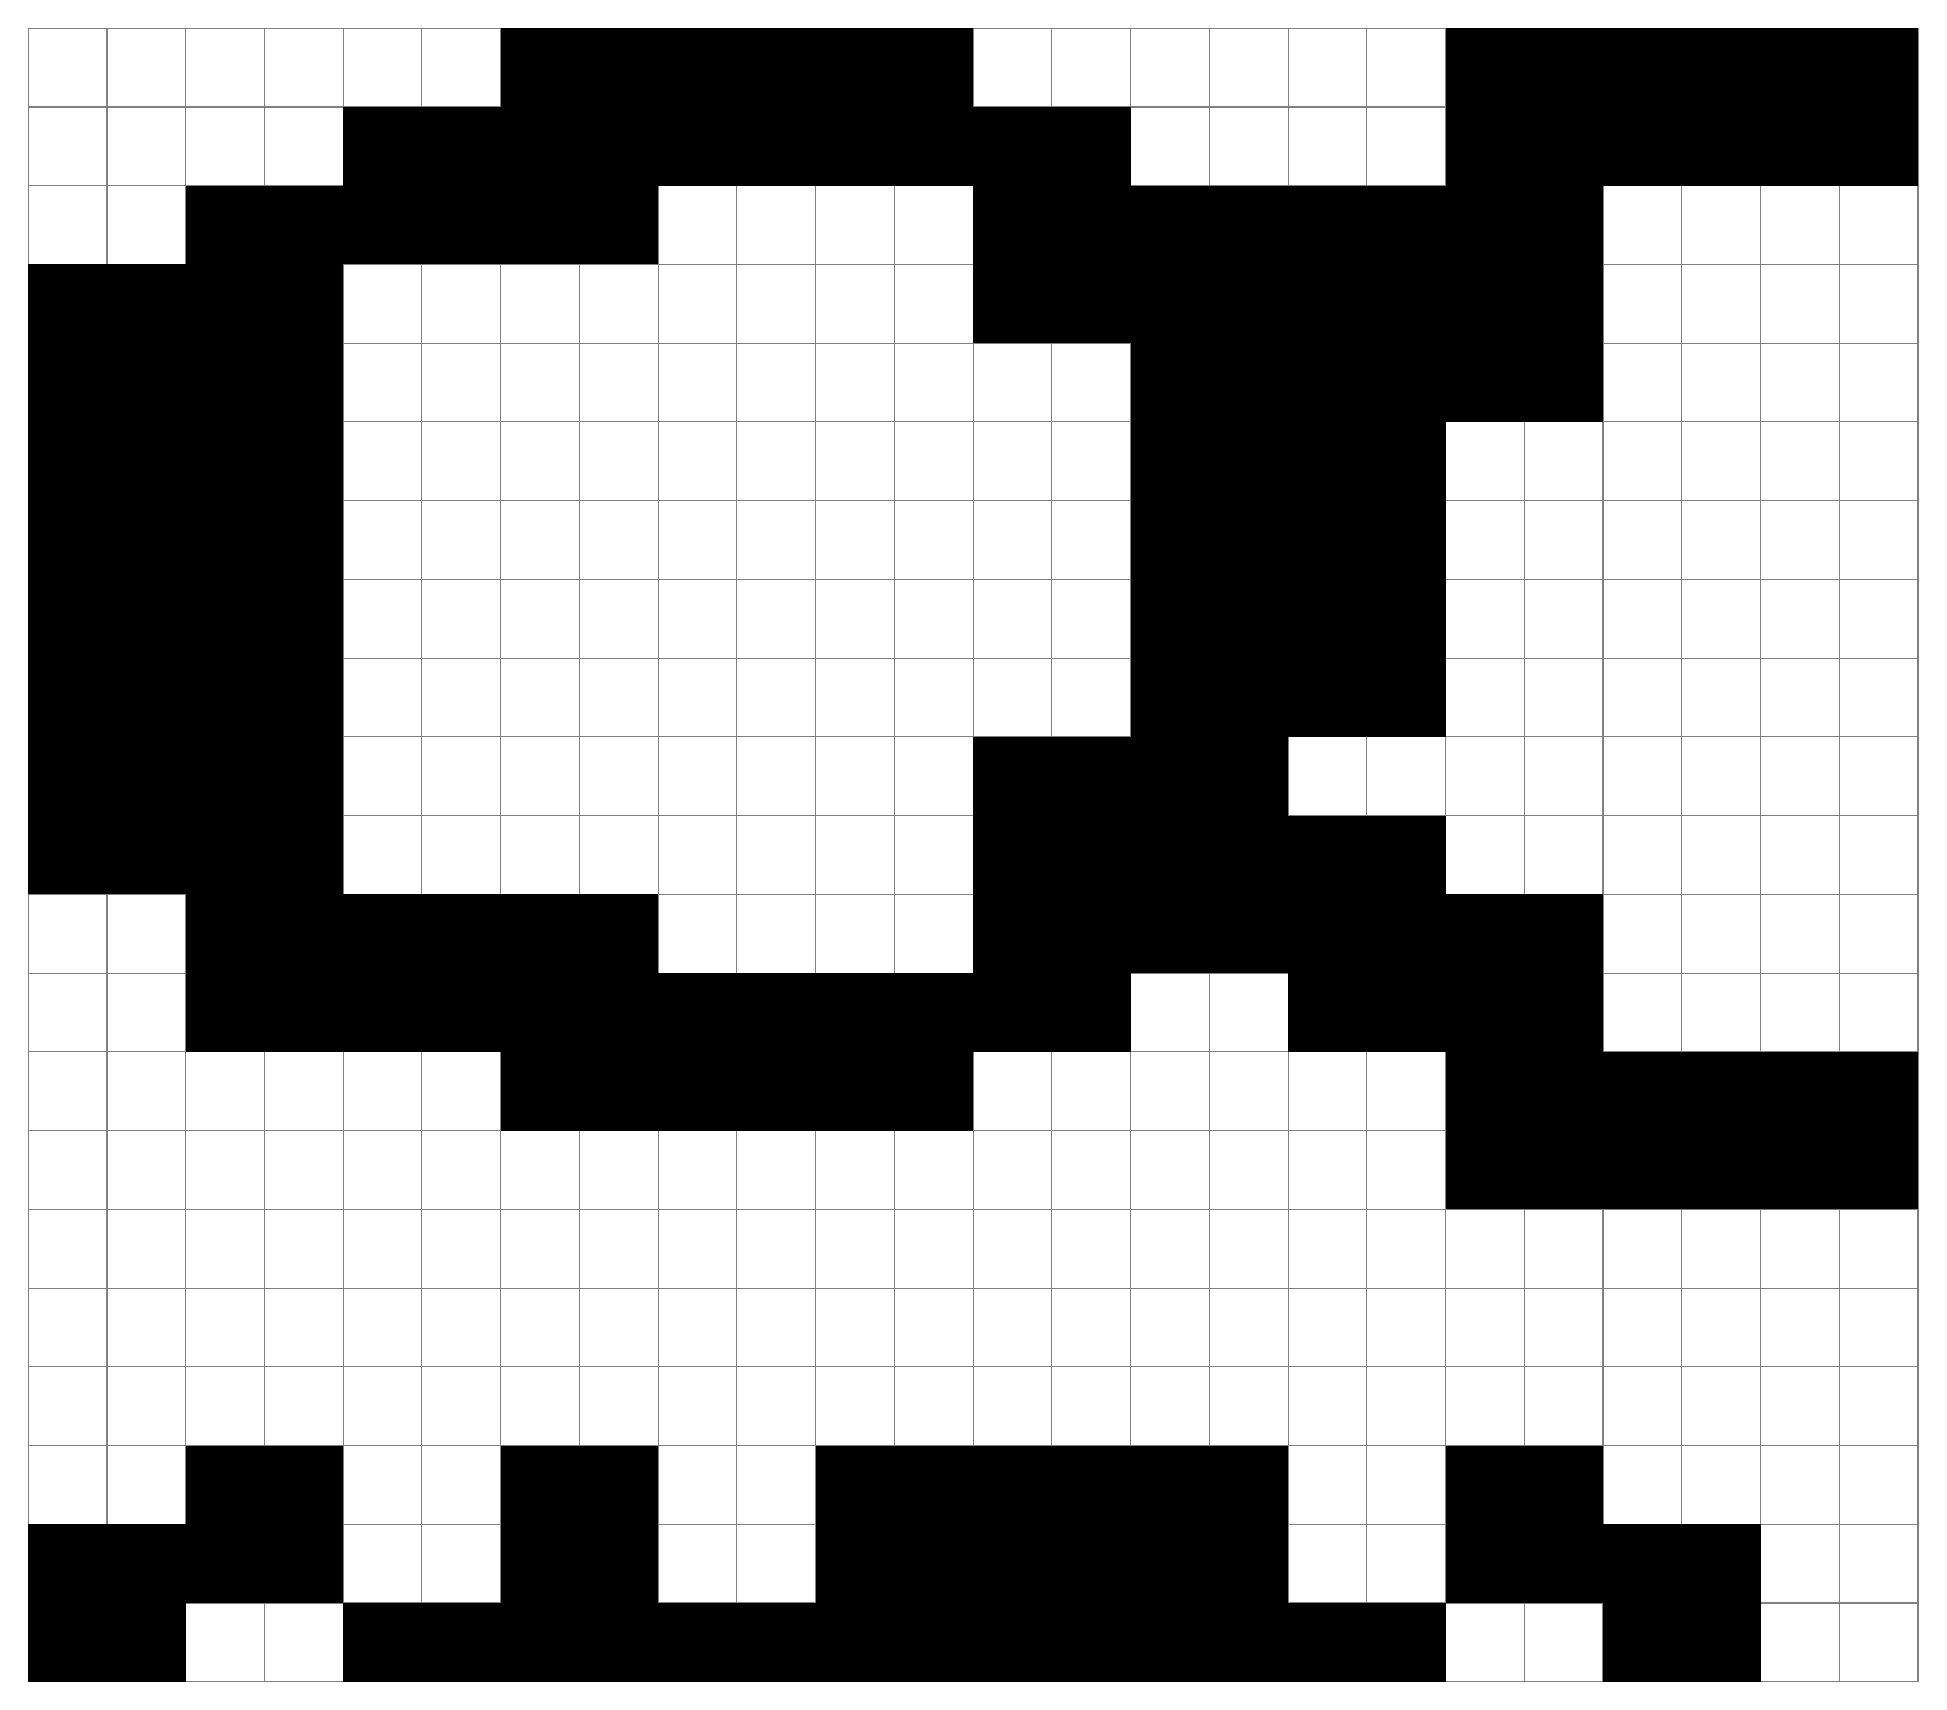
\begin{tikzpicture}

	\draw[step=1.0,gray,thin] (0,0) grid (24,21);
	\fill[\MULTICOLORONE] (6,20) rectangle ++ (1,1);
	\fill[\MULTICOLORONE] (7,20) rectangle ++ (1,1);
	\fill[\MULTICOLORTWO] (8,20) rectangle ++ (1,1);
	\fill[\MULTICOLORTWO] (9,20) rectangle ++ (1,1);
	\fill[\SPRITECOLOR] (10,20) rectangle ++ (1,1);
	\fill[\SPRITECOLOR] (11,20) rectangle ++ (1,1);
	\fill[\MULTICOLORONE] (18,20) rectangle ++ (1,1);
	\fill[\MULTICOLORONE] (19,20) rectangle ++ (1,1);
	\fill[\MULTICOLORTWO] (20,20) rectangle ++ (1,1);
	\fill[\MULTICOLORTWO] (21,20) rectangle ++ (1,1);
	\fill[\SPRITECOLOR] (22,20) rectangle ++ (1,1);
	\fill[\SPRITECOLOR] (23,20) rectangle ++ (1,1);
	\fill[\MULTICOLORTWO] (4,19) rectangle ++ (1,1);
	\fill[\MULTICOLORTWO] (5,19) rectangle ++ (1,1);
	\fill[\MULTICOLORTWO] (6,19) rectangle ++ (1,1);
	\fill[\MULTICOLORTWO] (7,19) rectangle ++ (1,1);
	\fill[\MULTICOLORTWO] (8,19) rectangle ++ (1,1);
	\fill[\MULTICOLORTWO] (9,19) rectangle ++ (1,1);
	\fill[\MULTICOLORTWO] (10,19) rectangle ++ (1,1);
	\fill[\MULTICOLORTWO] (11,19) rectangle ++ (1,1);
	\fill[\MULTICOLORTWO] (12,19) rectangle ++ (1,1);
	\fill[\MULTICOLORTWO] (13,19) rectangle ++ (1,1);
	\fill[\MULTICOLORTWO] (18,19) rectangle ++ (1,1);
	\fill[\MULTICOLORTWO] (19,19) rectangle ++ (1,1);
	\fill[\MULTICOLORTWO] (20,19) rectangle ++ (1,1);
	\fill[\MULTICOLORTWO] (21,19) rectangle ++ (1,1);
	\fill[\MULTICOLORTWO] (22,19) rectangle ++ (1,1);
	\fill[\MULTICOLORTWO] (23,19) rectangle ++ (1,1);
	\fill[\MULTICOLORTWO] (2,18) rectangle ++ (1,1);
	\fill[\MULTICOLORTWO] (3,18) rectangle ++ (1,1);
	\fill[\MULTICOLORTWO] (4,18) rectangle ++ (1,1);
	\fill[\MULTICOLORTWO] (5,18) rectangle ++ (1,1);
	\fill[\SPRITECOLOR] (6,18) rectangle ++ (1,1);
	\fill[\SPRITECOLOR] (7,18) rectangle ++ (1,1);
	\fill[\MULTICOLORTWO] (12,18) rectangle ++ (1,1);
	\fill[\MULTICOLORTWO] (13,18) rectangle ++ (1,1);
	\fill[\SPRITECOLOR] (14,18) rectangle ++ (1,1);
	\fill[\SPRITECOLOR] (15,18) rectangle ++ (1,1);
	\fill[\MULTICOLORONE] (16,18) rectangle ++ (1,1);
	\fill[\MULTICOLORONE] (17,18) rectangle ++ (1,1);
	\fill[\MULTICOLORTWO] (18,18) rectangle ++ (1,1);
	\fill[\MULTICOLORTWO] (19,18) rectangle ++ (1,1);
	\fill[\MULTICOLORONE] (0,17) rectangle ++ (1,1);
	\fill[\MULTICOLORONE] (1,17) rectangle ++ (1,1);
	\fill[\MULTICOLORTWO] (2,17) rectangle ++ (1,1);
	\fill[\MULTICOLORTWO] (3,17) rectangle ++ (1,1);
	\fill[\MULTICOLORONE] (12,17) rectangle ++ (1,1);
	\fill[\MULTICOLORONE] (13,17) rectangle ++ (1,1);
	\fill[\SPRITECOLOR] (14,17) rectangle ++ (1,1);
	\fill[\SPRITECOLOR] (15,17) rectangle ++ (1,1);
	\fill[\MULTICOLORTWO] (16,17) rectangle ++ (1,1);
	\fill[\MULTICOLORTWO] (17,17) rectangle ++ (1,1);
	\fill[\SPRITECOLOR] (18,17) rectangle ++ (1,1);
	\fill[\SPRITECOLOR] (19,17) rectangle ++ (1,1);
	\fill[\MULTICOLORONE] (0,16) rectangle ++ (1,1);
	\fill[\MULTICOLORONE] (1,16) rectangle ++ (1,1);
	\fill[\MULTICOLORTWO] (2,16) rectangle ++ (1,1);
	\fill[\MULTICOLORTWO] (3,16) rectangle ++ (1,1);
	\fill[\SPRITECOLOR] (14,16) rectangle ++ (1,1);
	\fill[\SPRITECOLOR] (15,16) rectangle ++ (1,1);
	\fill[\MULTICOLORTWO] (16,16) rectangle ++ (1,1);
	\fill[\MULTICOLORTWO] (17,16) rectangle ++ (1,1);
	\fill[\SPRITECOLOR] (18,16) rectangle ++ (1,1);
	\fill[\SPRITECOLOR] (19,16) rectangle ++ (1,1);
	\fill[\MULTICOLORTWO] (0,15) rectangle ++ (1,1);
	\fill[\MULTICOLORTWO] (1,15) rectangle ++ (1,1);
	\fill[\SPRITECOLOR] (2,15) rectangle ++ (1,1);
	\fill[\SPRITECOLOR] (3,15) rectangle ++ (1,1);
	\fill[\MULTICOLORONE] (14,15) rectangle ++ (1,1);
	\fill[\MULTICOLORONE] (15,15) rectangle ++ (1,1);
	\fill[\MULTICOLORTWO] (16,15) rectangle ++ (1,1);
	\fill[\MULTICOLORTWO] (17,15) rectangle ++ (1,1);
	\fill[\MULTICOLORTWO] (0,14) rectangle ++ (1,1);
	\fill[\MULTICOLORTWO] (1,14) rectangle ++ (1,1);
	\fill[\SPRITECOLOR] (2,14) rectangle ++ (1,1);
	\fill[\SPRITECOLOR] (3,14) rectangle ++ (1,1);
	\fill[\MULTICOLORONE] (14,14) rectangle ++ (1,1);
	\fill[\MULTICOLORONE] (15,14) rectangle ++ (1,1);
	\fill[\MULTICOLORTWO] (16,14) rectangle ++ (1,1);
	\fill[\MULTICOLORTWO] (17,14) rectangle ++ (1,1);
	\fill[\MULTICOLORTWO] (0,13) rectangle ++ (1,1);
	\fill[\MULTICOLORTWO] (1,13) rectangle ++ (1,1);
	\fill[\SPRITECOLOR] (2,13) rectangle ++ (1,1);
	\fill[\SPRITECOLOR] (3,13) rectangle ++ (1,1);
	\fill[\MULTICOLORTWO] (14,13) rectangle ++ (1,1);
	\fill[\MULTICOLORTWO] (15,13) rectangle ++ (1,1);
	\fill[\SPRITECOLOR] (16,13) rectangle ++ (1,1);
	\fill[\SPRITECOLOR] (17,13) rectangle ++ (1,1);
	\fill[\MULTICOLORTWO] (0,12) rectangle ++ (1,1);
	\fill[\MULTICOLORTWO] (1,12) rectangle ++ (1,1);
	\fill[\SPRITECOLOR] (2,12) rectangle ++ (1,1);
	\fill[\SPRITECOLOR] (3,12) rectangle ++ (1,1);
	\fill[\MULTICOLORTWO] (14,12) rectangle ++ (1,1);
	\fill[\MULTICOLORTWO] (15,12) rectangle ++ (1,1);
	\fill[\SPRITECOLOR] (16,12) rectangle ++ (1,1);
	\fill[\SPRITECOLOR] (17,12) rectangle ++ (1,1);
	\fill[\MULTICOLORONE] (0,11) rectangle ++ (1,1);
	\fill[\MULTICOLORONE] (1,11) rectangle ++ (1,1);
	\fill[\MULTICOLORTWO] (2,11) rectangle ++ (1,1);
	\fill[\MULTICOLORTWO] (3,11) rectangle ++ (1,1);
	\fill[\MULTICOLORONE] (12,11) rectangle ++ (1,1);
	\fill[\MULTICOLORONE] (13,11) rectangle ++ (1,1);
	\fill[\MULTICOLORTWO] (14,11) rectangle ++ (1,1);
	\fill[\MULTICOLORTWO] (15,11) rectangle ++ (1,1);
	\fill[\MULTICOLORONE] (0,10) rectangle ++ (1,1);
	\fill[\MULTICOLORONE] (1,10) rectangle ++ (1,1);
	\fill[\MULTICOLORTWO] (2,10) rectangle ++ (1,1);
	\fill[\MULTICOLORTWO] (3,10) rectangle ++ (1,1);
	\fill[\MULTICOLORONE] (12,10) rectangle ++ (1,1);
	\fill[\MULTICOLORONE] (13,10) rectangle ++ (1,1);
	\fill[\MULTICOLORTWO] (14,10) rectangle ++ (1,1);
	\fill[\MULTICOLORTWO] (15,10) rectangle ++ (1,1);
	\fill[\MULTICOLORONE] (16,10) rectangle ++ (1,1);
	\fill[\MULTICOLORONE] (17,10) rectangle ++ (1,1);
	\fill[\MULTICOLORTWO] (2,9) rectangle ++ (1,1);
	\fill[\MULTICOLORTWO] (3,9) rectangle ++ (1,1);
	\fill[\MULTICOLORTWO] (4,9) rectangle ++ (1,1);
	\fill[\MULTICOLORTWO] (5,9) rectangle ++ (1,1);
	\fill[\SPRITECOLOR] (6,9) rectangle ++ (1,1);
	\fill[\SPRITECOLOR] (7,9) rectangle ++ (1,1);
	\fill[\MULTICOLORTWO] (12,9) rectangle ++ (1,1);
	\fill[\MULTICOLORTWO] (13,9) rectangle ++ (1,1);
	\fill[\SPRITECOLOR] (14,9) rectangle ++ (1,1);
	\fill[\SPRITECOLOR] (15,9) rectangle ++ (1,1);
	\fill[\MULTICOLORONE] (16,9) rectangle ++ (1,1);
	\fill[\MULTICOLORONE] (17,9) rectangle ++ (1,1);
	\fill[\SPRITECOLOR] (18,9) rectangle ++ (1,1);
	\fill[\SPRITECOLOR] (19,9) rectangle ++ (1,1);
	\fill[\MULTICOLORONE] (2,8) rectangle ++ (1,1);
	\fill[\MULTICOLORONE] (3,8) rectangle ++ (1,1);
	\fill[\MULTICOLORTWO] (4,8) rectangle ++ (1,1);
	\fill[\MULTICOLORTWO] (5,8) rectangle ++ (1,1);
	\fill[\MULTICOLORTWO] (6,8) rectangle ++ (1,1);
	\fill[\MULTICOLORTWO] (7,8) rectangle ++ (1,1);
	\fill[\MULTICOLORTWO] (8,8) rectangle ++ (1,1);
	\fill[\MULTICOLORTWO] (9,8) rectangle ++ (1,1);
	\fill[\MULTICOLORTWO] (10,8) rectangle ++ (1,1);
	\fill[\MULTICOLORTWO] (11,8) rectangle ++ (1,1);
	\fill[\MULTICOLORTWO] (12,8) rectangle ++ (1,1);
	\fill[\MULTICOLORTWO] (13,8) rectangle ++ (1,1);
	\fill[\MULTICOLORONE] (16,8) rectangle ++ (1,1);
	\fill[\MULTICOLORONE] (17,8) rectangle ++ (1,1);
	\fill[\MULTICOLORTWO] (18,8) rectangle ++ (1,1);
	\fill[\MULTICOLORTWO] (19,8) rectangle ++ (1,1);
	\fill[\MULTICOLORONE] (6,7) rectangle ++ (1,1);
	\fill[\MULTICOLORONE] (7,7) rectangle ++ (1,1);
	\fill[\MULTICOLORTWO] (8,7) rectangle ++ (1,1);
	\fill[\MULTICOLORTWO] (9,7) rectangle ++ (1,1);
	\fill[\SPRITECOLOR] (10,7) rectangle ++ (1,1);
	\fill[\SPRITECOLOR] (11,7) rectangle ++ (1,1);
	\fill[\MULTICOLORTWO] (18,7) rectangle ++ (1,1);
	\fill[\MULTICOLORTWO] (19,7) rectangle ++ (1,1);
	\fill[\MULTICOLORTWO] (20,7) rectangle ++ (1,1);
	\fill[\MULTICOLORTWO] (21,7) rectangle ++ (1,1);
	\fill[\MULTICOLORTWO] (22,7) rectangle ++ (1,1);
	\fill[\MULTICOLORTWO] (23,7) rectangle ++ (1,1);
	\fill[\MULTICOLORONE] (18,6) rectangle ++ (1,1);
	\fill[\MULTICOLORONE] (19,6) rectangle ++ (1,1);
	\fill[\MULTICOLORTWO] (20,6) rectangle ++ (1,1);
	\fill[\MULTICOLORTWO] (21,6) rectangle ++ (1,1);
	\fill[\SPRITECOLOR] (22,6) rectangle ++ (1,1);
	\fill[\SPRITECOLOR] (23,6) rectangle ++ (1,1);
	\fill[\SPRITECOLOR] (2,2) rectangle ++ (1,1);
	\fill[\SPRITECOLOR] (3,2) rectangle ++ (1,1);
	\fill[\SPRITECOLOR] (6,2) rectangle ++ (1,1);
	\fill[\SPRITECOLOR] (7,2) rectangle ++ (1,1);
	\fill[\MULTICOLORTWO] (10,2) rectangle ++ (1,1);
	\fill[\MULTICOLORTWO] (11,2) rectangle ++ (1,1);
	\fill[\MULTICOLORONE] (12,2) rectangle ++ (1,1);
	\fill[\MULTICOLORONE] (13,2) rectangle ++ (1,1);
	\fill[\MULTICOLORONE] (14,2) rectangle ++ (1,1);
	\fill[\MULTICOLORONE] (15,2) rectangle ++ (1,1);
	\fill[\MULTICOLORONE] (18,2) rectangle ++ (1,1);
	\fill[\MULTICOLORONE] (19,2) rectangle ++ (1,1);
	\fill[\MULTICOLORONE] (0,1) rectangle ++ (1,1);
	\fill[\MULTICOLORONE] (1,1) rectangle ++ (1,1);
	\fill[\MULTICOLORONE] (2,1) rectangle ++ (1,1);
	\fill[\MULTICOLORONE] (3,1) rectangle ++ (1,1);
	\fill[\SPRITECOLOR] (6,1) rectangle ++ (1,1);
	\fill[\SPRITECOLOR] (7,1) rectangle ++ (1,1);
	\fill[\MULTICOLORTWO] (10,1) rectangle ++ (1,1);
	\fill[\MULTICOLORTWO] (11,1) rectangle ++ (1,1);
	\fill[\MULTICOLORONE] (12,1) rectangle ++ (1,1);
	\fill[\MULTICOLORONE] (13,1) rectangle ++ (1,1);
	\fill[\MULTICOLORTWO] (14,1) rectangle ++ (1,1);
	\fill[\MULTICOLORTWO] (15,1) rectangle ++ (1,1);
	\fill[\SPRITECOLOR] (18,1) rectangle ++ (1,1);
	\fill[\SPRITECOLOR] (19,1) rectangle ++ (1,1);
	\fill[\SPRITECOLOR] (20,1) rectangle ++ (1,1);
	\fill[\SPRITECOLOR] (21,1) rectangle ++ (1,1);
	\fill[\SPRITECOLOR] (0,0) rectangle ++ (1,1);
	\fill[\SPRITECOLOR] (1,0) rectangle ++ (1,1);
	\fill[\SPRITECOLOR] (4,0) rectangle ++ (1,1);
	\fill[\SPRITECOLOR] (5,0) rectangle ++ (1,1);
	\fill[\MULTICOLORTWO] (6,0) rectangle ++ (1,1);
	\fill[\MULTICOLORTWO] (7,0) rectangle ++ (1,1);
	\fill[\SPRITECOLOR] (8,0) rectangle ++ (1,1);
	\fill[\SPRITECOLOR] (9,0) rectangle ++ (1,1);
	\fill[\SPRITECOLOR] (10,0) rectangle ++ (1,1);
	\fill[\SPRITECOLOR] (11,0) rectangle ++ (1,1);
	\fill[\MULTICOLORONE] (12,0) rectangle ++ (1,1);
	\fill[\MULTICOLORONE] (13,0) rectangle ++ (1,1);
	\fill[\MULTICOLORONE] (14,0) rectangle ++ (1,1);
	\fill[\MULTICOLORONE] (15,0) rectangle ++ (1,1);
	\fill[\MULTICOLORONE] (16,0) rectangle ++ (1,1);
	\fill[\MULTICOLORONE] (17,0) rectangle ++ (1,1);
	\fill[\MULTICOLORONE] (20,0) rectangle ++ (1,1);
	\fill[\MULTICOLORONE] (21,0) rectangle ++ (1,1);

      \end{tikzpicture}
    \end{adjustbox}
  }\caption{ALPHA}
\end{figure}

	\end{subfigure}
} \\ 
        \midrule
\makecell[l]{
	\begin{subfigure}{0.3\textwidth}
    \def\MULTICOLORONE{gray}
    \def\MULTICOLORTWO{white}
    \def\SPRITECOLOR{red}
		
\begin{figure}[H]
  {
    \setlength{\tabcolsep}{3.0pt}
    \setlength\cmidrulewidth{\heavyrulewidth} % Make cmidrule = 
    \begin{adjustbox}{width=3cm,center}
      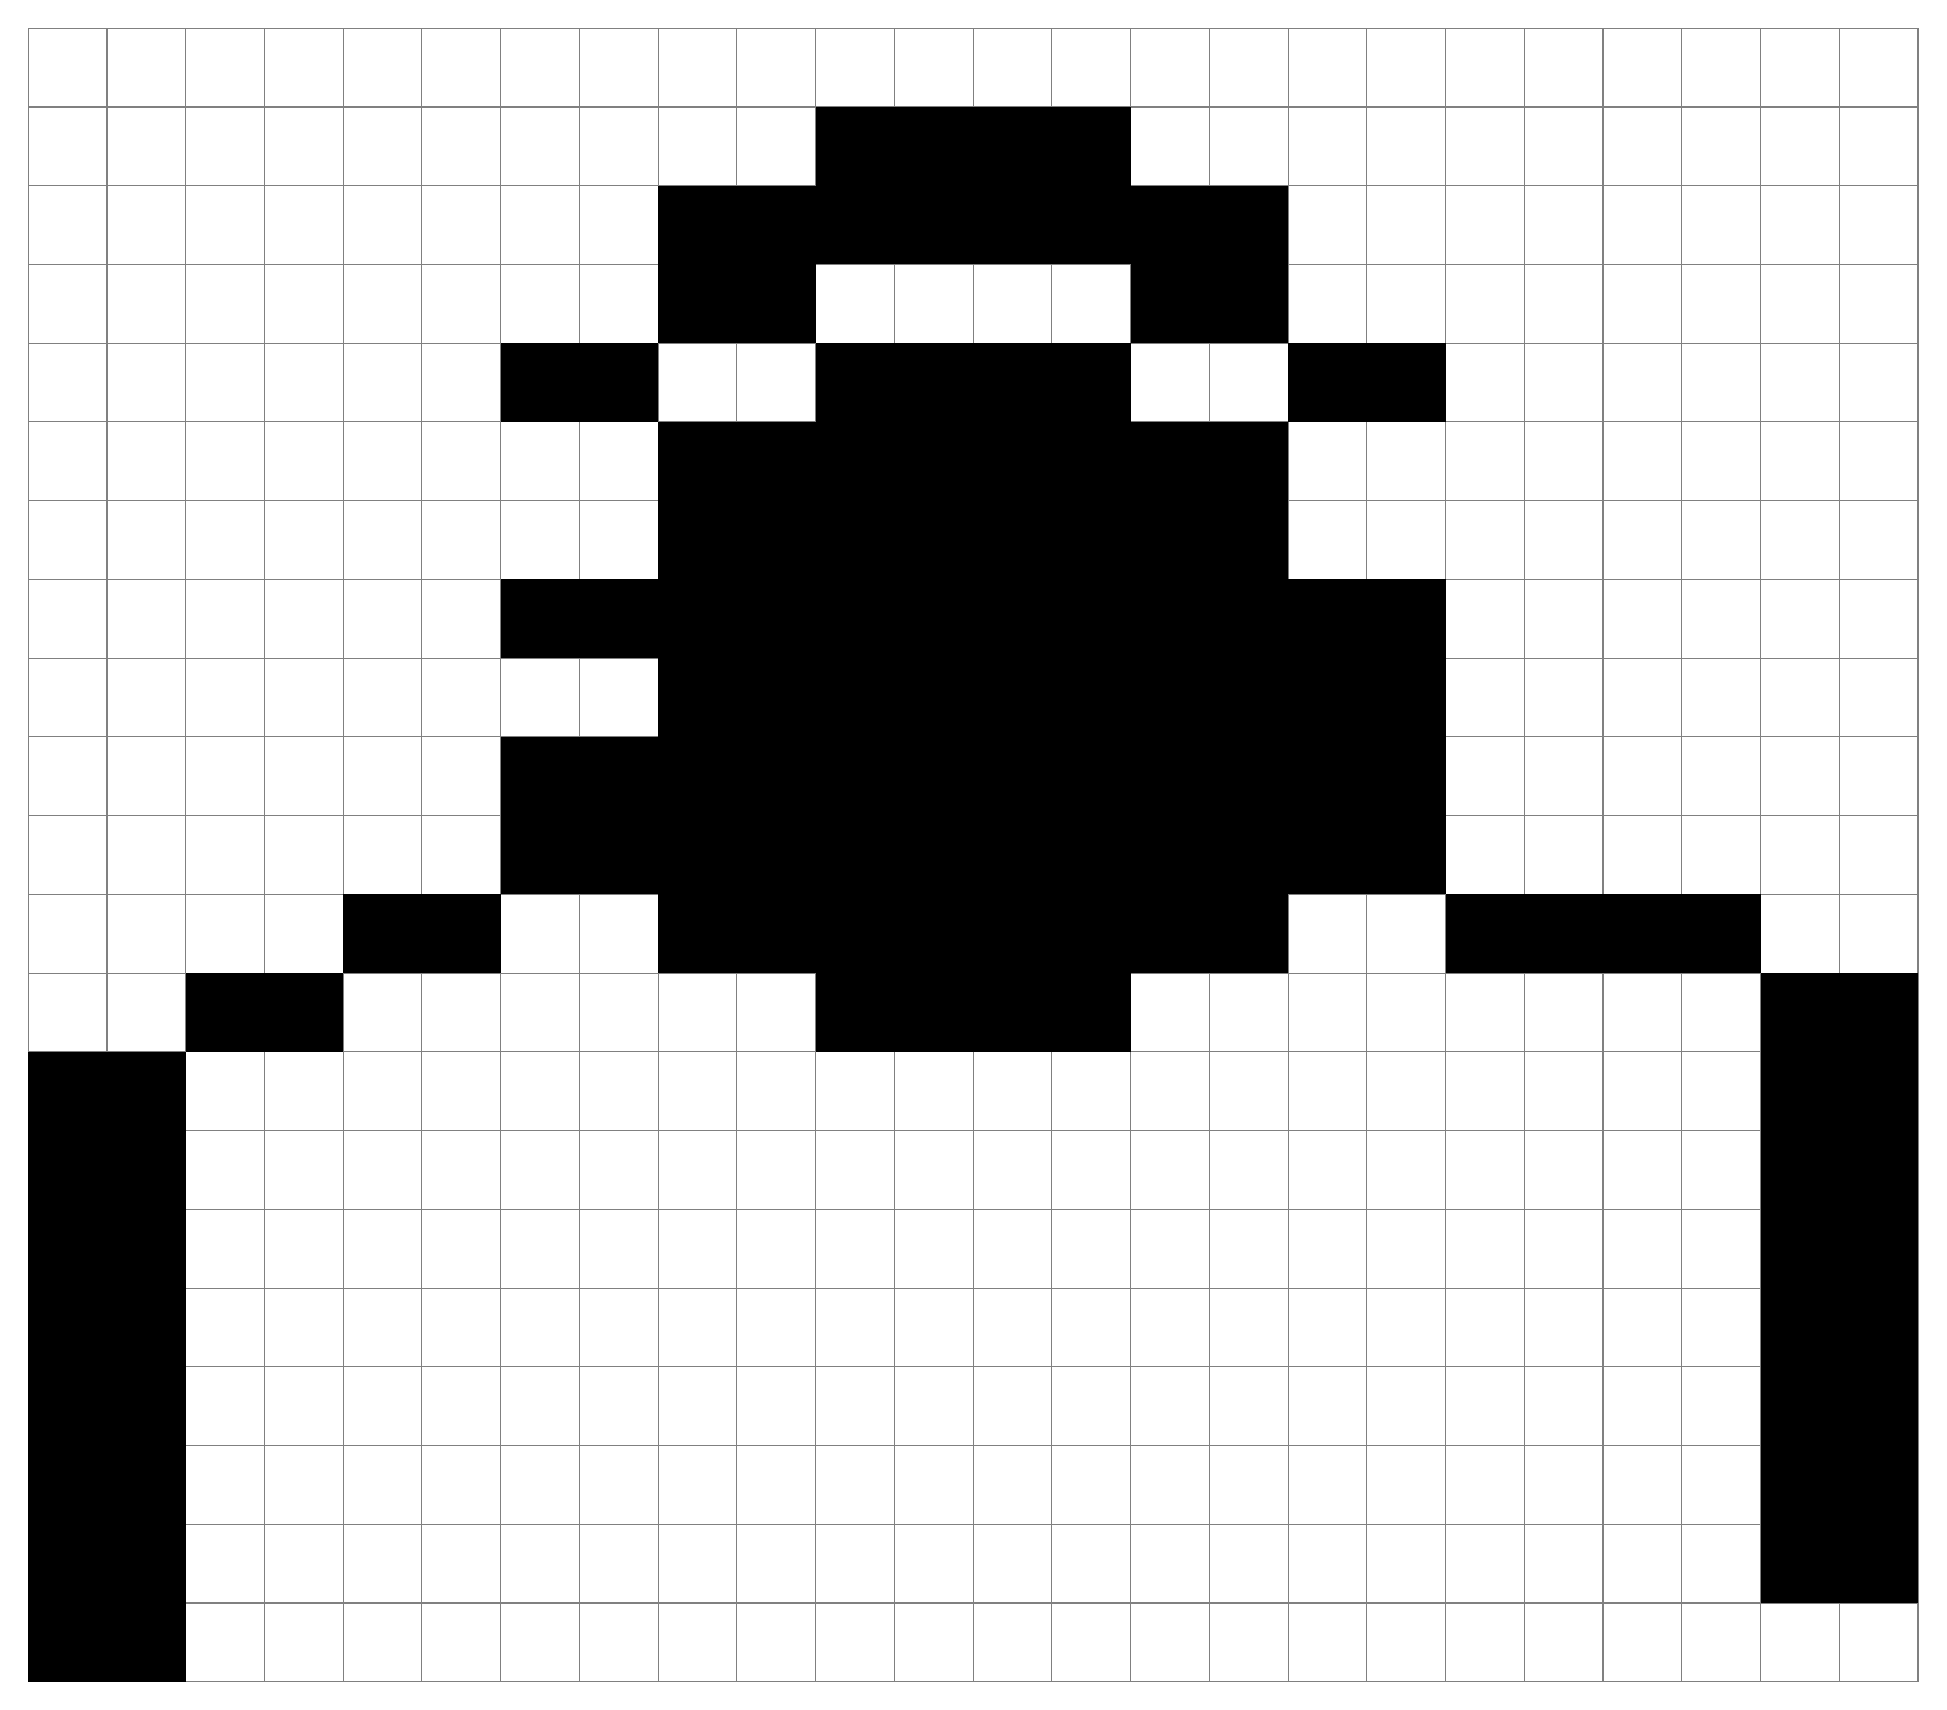
\begin{tikzpicture}

	\draw[step=1.0,gray,thin] (0,0) grid (24,21);
	\fill[\SPRITECOLOR] (10,19) rectangle ++ (1,1);
	\fill[\SPRITECOLOR] (11,19) rectangle ++ (1,1);
	\fill[\SPRITECOLOR] (12,19) rectangle ++ (1,1);
	\fill[\SPRITECOLOR] (13,19) rectangle ++ (1,1);
	\fill[\SPRITECOLOR] (8,18) rectangle ++ (1,1);
	\fill[\SPRITECOLOR] (9,18) rectangle ++ (1,1);
	\fill[\SPRITECOLOR] (10,18) rectangle ++ (1,1);
	\fill[\SPRITECOLOR] (11,18) rectangle ++ (1,1);
	\fill[\SPRITECOLOR] (12,18) rectangle ++ (1,1);
	\fill[\SPRITECOLOR] (13,18) rectangle ++ (1,1);
	\fill[\SPRITECOLOR] (14,18) rectangle ++ (1,1);
	\fill[\SPRITECOLOR] (15,18) rectangle ++ (1,1);
	\fill[\SPRITECOLOR] (8,17) rectangle ++ (1,1);
	\fill[\SPRITECOLOR] (9,17) rectangle ++ (1,1);
	\fill[\SPRITECOLOR] (14,17) rectangle ++ (1,1);
	\fill[\SPRITECOLOR] (15,17) rectangle ++ (1,1);
	\fill[\SPRITECOLOR] (6,16) rectangle ++ (1,1);
	\fill[\SPRITECOLOR] (7,16) rectangle ++ (1,1);
	\fill[\SPRITECOLOR] (10,16) rectangle ++ (1,1);
	\fill[\SPRITECOLOR] (11,16) rectangle ++ (1,1);
	\fill[\SPRITECOLOR] (12,16) rectangle ++ (1,1);
	\fill[\SPRITECOLOR] (13,16) rectangle ++ (1,1);
	\fill[\SPRITECOLOR] (16,16) rectangle ++ (1,1);
	\fill[\SPRITECOLOR] (17,16) rectangle ++ (1,1);
	\fill[\SPRITECOLOR] (8,15) rectangle ++ (1,1);
	\fill[\SPRITECOLOR] (9,15) rectangle ++ (1,1);
	\fill[\MULTICOLORTWO] (10,15) rectangle ++ (1,1);
	\fill[\MULTICOLORTWO] (11,15) rectangle ++ (1,1);
	\fill[\SPRITECOLOR] (12,15) rectangle ++ (1,1);
	\fill[\SPRITECOLOR] (13,15) rectangle ++ (1,1);
	\fill[\SPRITECOLOR] (14,15) rectangle ++ (1,1);
	\fill[\SPRITECOLOR] (15,15) rectangle ++ (1,1);
	\fill[\MULTICOLORTWO] (8,14) rectangle ++ (1,1);
	\fill[\MULTICOLORTWO] (9,14) rectangle ++ (1,1);
	\fill[\SPRITECOLOR] (10,14) rectangle ++ (1,1);
	\fill[\SPRITECOLOR] (11,14) rectangle ++ (1,1);
	\fill[\SPRITECOLOR] (12,14) rectangle ++ (1,1);
	\fill[\SPRITECOLOR] (13,14) rectangle ++ (1,1);
	\fill[\SPRITECOLOR] (14,14) rectangle ++ (1,1);
	\fill[\SPRITECOLOR] (15,14) rectangle ++ (1,1);
	\fill[\MULTICOLORTWO] (6,13) rectangle ++ (1,1);
	\fill[\MULTICOLORTWO] (7,13) rectangle ++ (1,1);
	\fill[\MULTICOLORTWO] (8,13) rectangle ++ (1,1);
	\fill[\MULTICOLORTWO] (9,13) rectangle ++ (1,1);
	\fill[\SPRITECOLOR] (10,13) rectangle ++ (1,1);
	\fill[\SPRITECOLOR] (11,13) rectangle ++ (1,1);
	\fill[\SPRITECOLOR] (12,13) rectangle ++ (1,1);
	\fill[\SPRITECOLOR] (13,13) rectangle ++ (1,1);
	\fill[\SPRITECOLOR] (14,13) rectangle ++ (1,1);
	\fill[\SPRITECOLOR] (15,13) rectangle ++ (1,1);
	\fill[\SPRITECOLOR] (16,13) rectangle ++ (1,1);
	\fill[\SPRITECOLOR] (17,13) rectangle ++ (1,1);
	\fill[\MULTICOLORTWO] (8,12) rectangle ++ (1,1);
	\fill[\MULTICOLORTWO] (9,12) rectangle ++ (1,1);
	\fill[\SPRITECOLOR] (10,12) rectangle ++ (1,1);
	\fill[\SPRITECOLOR] (11,12) rectangle ++ (1,1);
	\fill[\SPRITECOLOR] (12,12) rectangle ++ (1,1);
	\fill[\SPRITECOLOR] (13,12) rectangle ++ (1,1);
	\fill[\SPRITECOLOR] (14,12) rectangle ++ (1,1);
	\fill[\SPRITECOLOR] (15,12) rectangle ++ (1,1);
	\fill[\SPRITECOLOR] (16,12) rectangle ++ (1,1);
	\fill[\SPRITECOLOR] (17,12) rectangle ++ (1,1);
	\fill[\MULTICOLORTWO] (6,11) rectangle ++ (1,1);
	\fill[\MULTICOLORTWO] (7,11) rectangle ++ (1,1);
	\fill[\MULTICOLORTWO] (8,11) rectangle ++ (1,1);
	\fill[\MULTICOLORTWO] (9,11) rectangle ++ (1,1);
	\fill[\SPRITECOLOR] (10,11) rectangle ++ (1,1);
	\fill[\SPRITECOLOR] (11,11) rectangle ++ (1,1);
	\fill[\SPRITECOLOR] (12,11) rectangle ++ (1,1);
	\fill[\SPRITECOLOR] (13,11) rectangle ++ (1,1);
	\fill[\SPRITECOLOR] (14,11) rectangle ++ (1,1);
	\fill[\SPRITECOLOR] (15,11) rectangle ++ (1,1);
	\fill[\SPRITECOLOR] (16,11) rectangle ++ (1,1);
	\fill[\SPRITECOLOR] (17,11) rectangle ++ (1,1);
	\fill[\MULTICOLORONE] (6,10) rectangle ++ (1,1);
	\fill[\MULTICOLORONE] (7,10) rectangle ++ (1,1);
	\fill[\SPRITECOLOR] (8,10) rectangle ++ (1,1);
	\fill[\SPRITECOLOR] (9,10) rectangle ++ (1,1);
	\fill[\SPRITECOLOR] (10,10) rectangle ++ (1,1);
	\fill[\SPRITECOLOR] (11,10) rectangle ++ (1,1);
	\fill[\SPRITECOLOR] (12,10) rectangle ++ (1,1);
	\fill[\SPRITECOLOR] (13,10) rectangle ++ (1,1);
	\fill[\SPRITECOLOR] (14,10) rectangle ++ (1,1);
	\fill[\SPRITECOLOR] (15,10) rectangle ++ (1,1);
	\fill[\MULTICOLORONE] (16,10) rectangle ++ (1,1);
	\fill[\MULTICOLORONE] (17,10) rectangle ++ (1,1);
	\fill[\MULTICOLORONE] (4,9) rectangle ++ (1,1);
	\fill[\MULTICOLORONE] (5,9) rectangle ++ (1,1);
	\fill[\SPRITECOLOR] (8,9) rectangle ++ (1,1);
	\fill[\SPRITECOLOR] (9,9) rectangle ++ (1,1);
	\fill[\SPRITECOLOR] (10,9) rectangle ++ (1,1);
	\fill[\SPRITECOLOR] (11,9) rectangle ++ (1,1);
	\fill[\SPRITECOLOR] (12,9) rectangle ++ (1,1);
	\fill[\SPRITECOLOR] (13,9) rectangle ++ (1,1);
	\fill[\SPRITECOLOR] (14,9) rectangle ++ (1,1);
	\fill[\SPRITECOLOR] (15,9) rectangle ++ (1,1);
	\fill[\MULTICOLORONE] (18,9) rectangle ++ (1,1);
	\fill[\MULTICOLORONE] (19,9) rectangle ++ (1,1);
	\fill[\MULTICOLORONE] (20,9) rectangle ++ (1,1);
	\fill[\MULTICOLORONE] (21,9) rectangle ++ (1,1);
	\fill[\MULTICOLORONE] (2,8) rectangle ++ (1,1);
	\fill[\MULTICOLORONE] (3,8) rectangle ++ (1,1);
	\fill[\SPRITECOLOR] (10,8) rectangle ++ (1,1);
	\fill[\SPRITECOLOR] (11,8) rectangle ++ (1,1);
	\fill[\SPRITECOLOR] (12,8) rectangle ++ (1,1);
	\fill[\SPRITECOLOR] (13,8) rectangle ++ (1,1);
	\fill[\MULTICOLORTWO] (22,8) rectangle ++ (1,1);
	\fill[\MULTICOLORTWO] (23,8) rectangle ++ (1,1);
	\fill[\MULTICOLORTWO] (0,7) rectangle ++ (1,1);
	\fill[\MULTICOLORTWO] (1,7) rectangle ++ (1,1);
	\fill[\MULTICOLORONE] (22,7) rectangle ++ (1,1);
	\fill[\MULTICOLORONE] (23,7) rectangle ++ (1,1);
	\fill[\MULTICOLORONE] (0,6) rectangle ++ (1,1);
	\fill[\MULTICOLORONE] (1,6) rectangle ++ (1,1);
	\fill[\MULTICOLORONE] (22,6) rectangle ++ (1,1);
	\fill[\MULTICOLORONE] (23,6) rectangle ++ (1,1);
	\fill[\MULTICOLORONE] (0,5) rectangle ++ (1,1);
	\fill[\MULTICOLORONE] (1,5) rectangle ++ (1,1);
	\fill[\MULTICOLORONE] (22,5) rectangle ++ (1,1);
	\fill[\MULTICOLORONE] (23,5) rectangle ++ (1,1);
	\fill[\MULTICOLORONE] (0,4) rectangle ++ (1,1);
	\fill[\MULTICOLORONE] (1,4) rectangle ++ (1,1);
	\fill[\MULTICOLORONE] (22,4) rectangle ++ (1,1);
	\fill[\MULTICOLORONE] (23,4) rectangle ++ (1,1);
	\fill[\MULTICOLORONE] (0,3) rectangle ++ (1,1);
	\fill[\MULTICOLORONE] (1,3) rectangle ++ (1,1);
	\fill[\MULTICOLORONE] (22,3) rectangle ++ (1,1);
	\fill[\MULTICOLORONE] (23,3) rectangle ++ (1,1);
	\fill[\MULTICOLORONE] (0,2) rectangle ++ (1,1);
	\fill[\MULTICOLORONE] (1,2) rectangle ++ (1,1);
	\fill[\MULTICOLORONE] (22,2) rectangle ++ (1,1);
	\fill[\MULTICOLORONE] (23,2) rectangle ++ (1,1);
	\fill[\MULTICOLORONE] (0,1) rectangle ++ (1,1);
	\fill[\MULTICOLORONE] (1,1) rectangle ++ (1,1);
	\fill[\MULTICOLORONE] (22,1) rectangle ++ (1,1);
	\fill[\MULTICOLORONE] (23,1) rectangle ++ (1,1);
	\fill[\MULTICOLORONE] (0,0) rectangle ++ (1,1);
	\fill[\MULTICOLORONE] (1,0) rectangle ++ (1,1);

      \end{tikzpicture}
    \end{adjustbox}
  }\caption{LAND\_GILBY1}
\end{figure}

	\end{subfigure}
} & 
\makecell[l]{
	\begin{subfigure}{0.3\textwidth}
    \def\MULTICOLORONE{gray}
    \def\MULTICOLORTWO{white}
    \def\SPRITECOLOR{red}
		
\begin{figure}[H]
  {
    \setlength{\tabcolsep}{3.0pt}
    \setlength\cmidrulewidth{\heavyrulewidth} % Make cmidrule = 
    \begin{adjustbox}{width=3cm,center}
      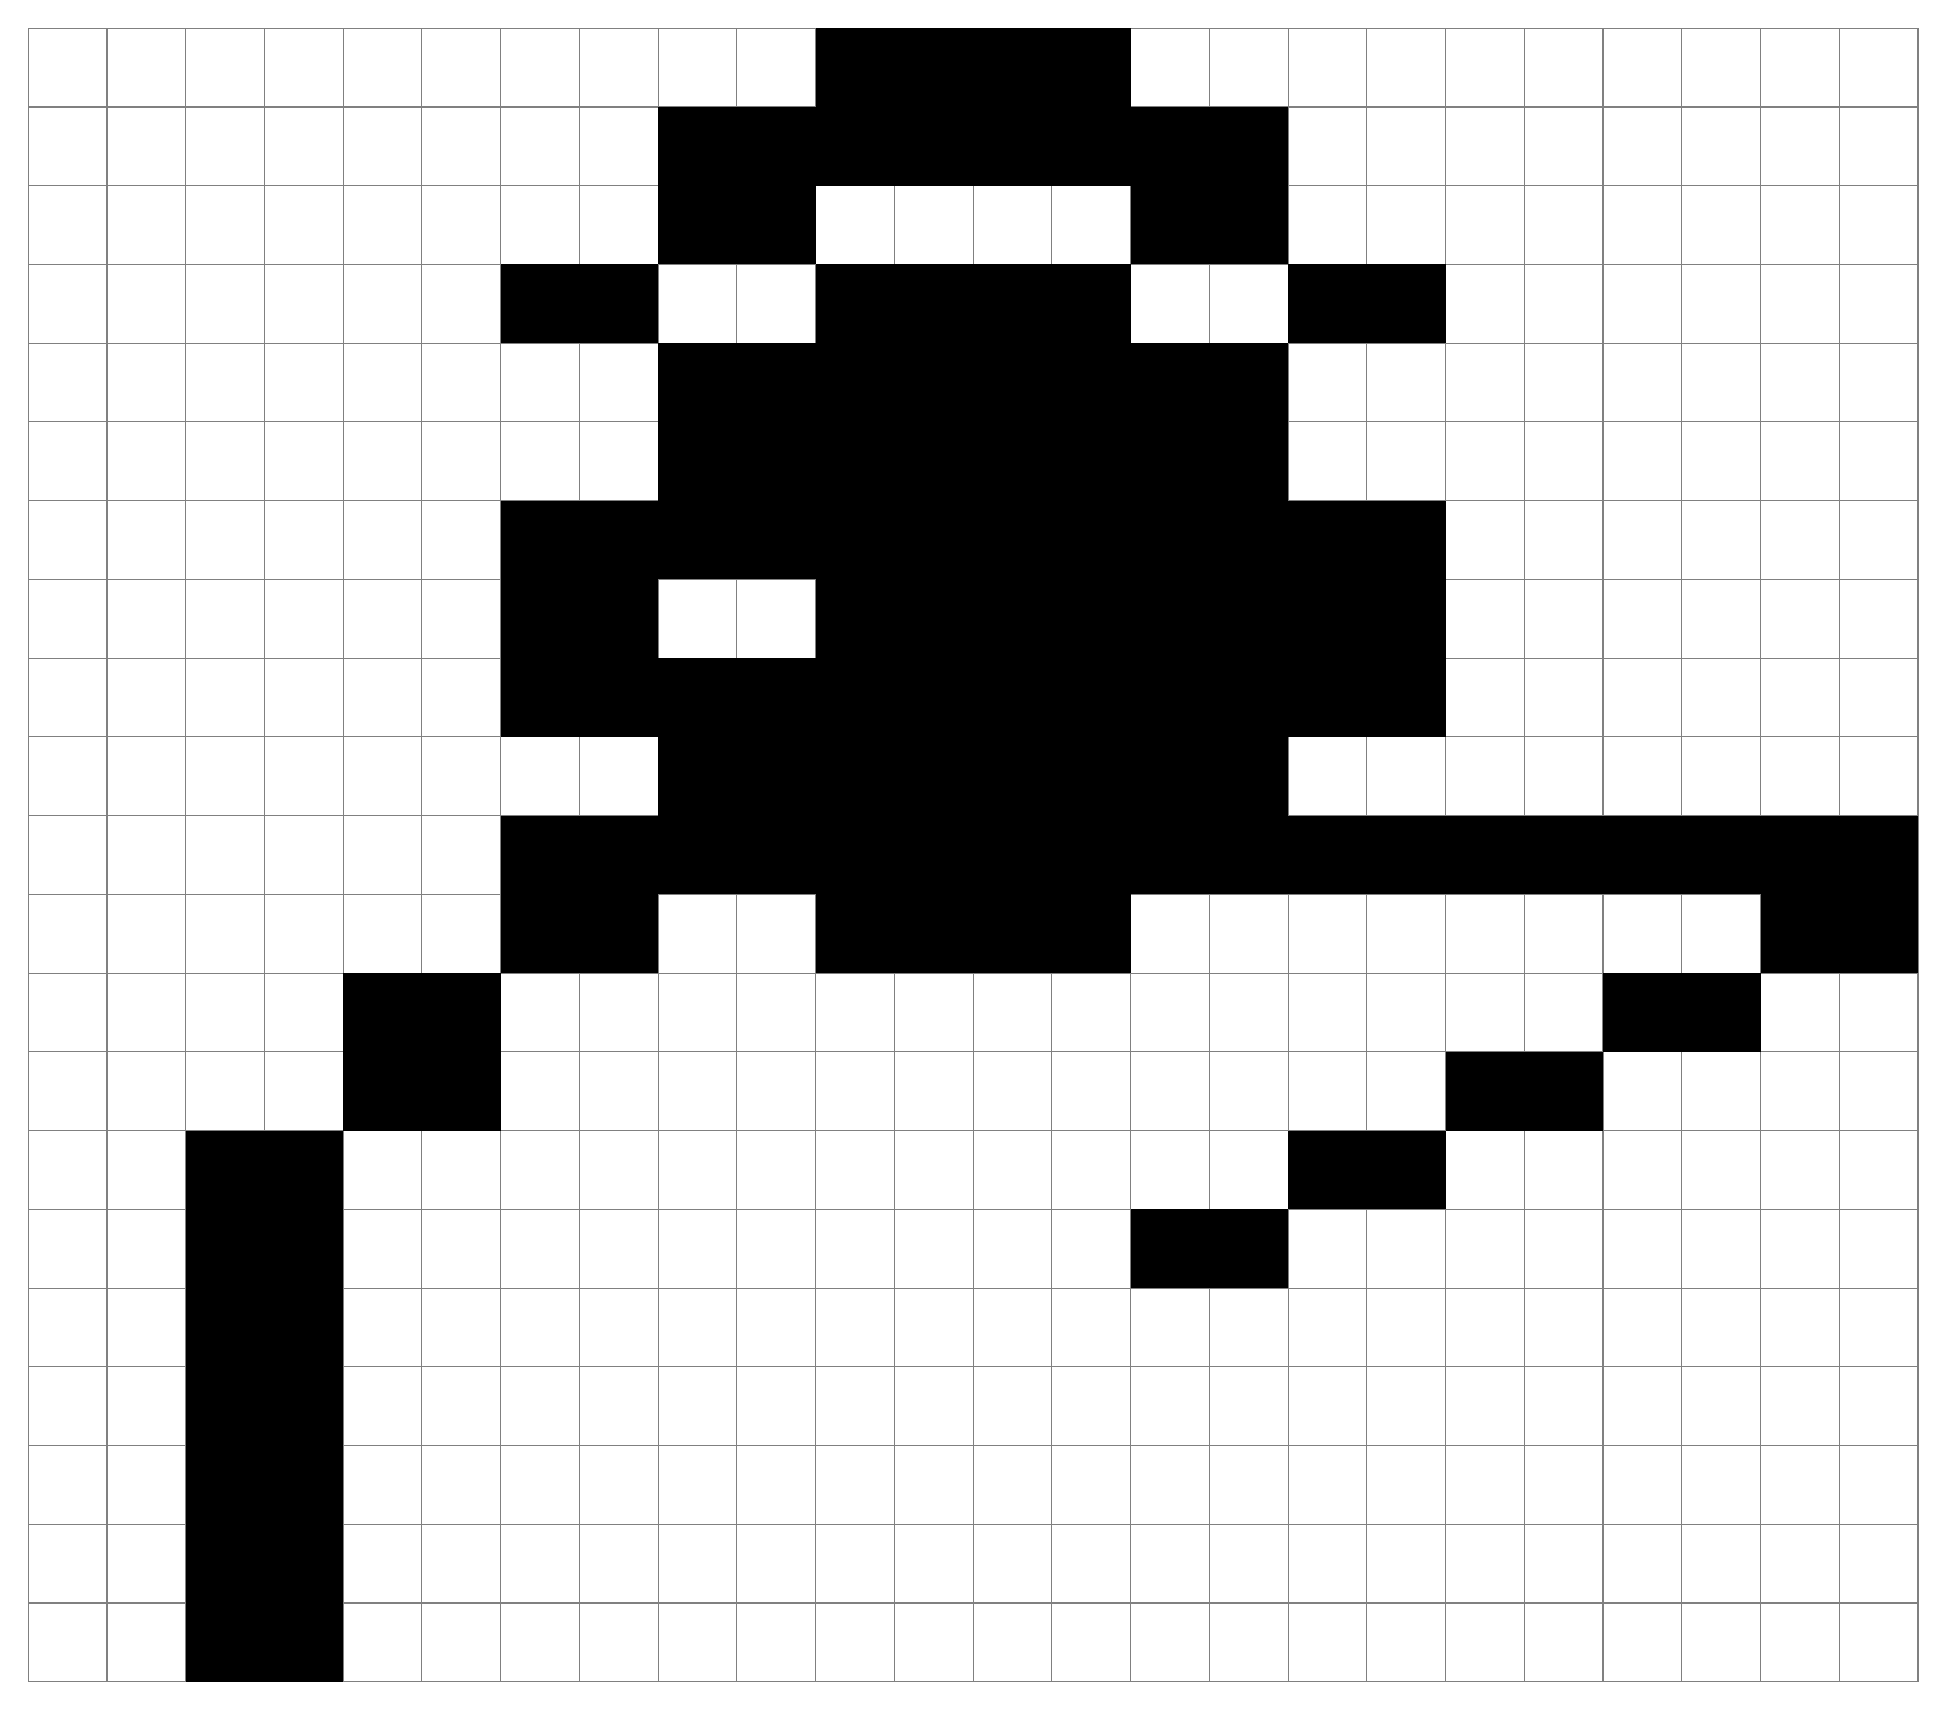
\begin{tikzpicture}

	\draw[step=1.0,gray,thin] (0,0) grid (24,21);
	\fill[\SPRITECOLOR] (10,20) rectangle ++ (1,1);
	\fill[\SPRITECOLOR] (11,20) rectangle ++ (1,1);
	\fill[\SPRITECOLOR] (12,20) rectangle ++ (1,1);
	\fill[\SPRITECOLOR] (13,20) rectangle ++ (1,1);
	\fill[\SPRITECOLOR] (8,19) rectangle ++ (1,1);
	\fill[\SPRITECOLOR] (9,19) rectangle ++ (1,1);
	\fill[\SPRITECOLOR] (10,19) rectangle ++ (1,1);
	\fill[\SPRITECOLOR] (11,19) rectangle ++ (1,1);
	\fill[\SPRITECOLOR] (12,19) rectangle ++ (1,1);
	\fill[\SPRITECOLOR] (13,19) rectangle ++ (1,1);
	\fill[\SPRITECOLOR] (14,19) rectangle ++ (1,1);
	\fill[\SPRITECOLOR] (15,19) rectangle ++ (1,1);
	\fill[\SPRITECOLOR] (8,18) rectangle ++ (1,1);
	\fill[\SPRITECOLOR] (9,18) rectangle ++ (1,1);
	\fill[\SPRITECOLOR] (14,18) rectangle ++ (1,1);
	\fill[\SPRITECOLOR] (15,18) rectangle ++ (1,1);
	\fill[\SPRITECOLOR] (6,17) rectangle ++ (1,1);
	\fill[\SPRITECOLOR] (7,17) rectangle ++ (1,1);
	\fill[\SPRITECOLOR] (10,17) rectangle ++ (1,1);
	\fill[\SPRITECOLOR] (11,17) rectangle ++ (1,1);
	\fill[\SPRITECOLOR] (12,17) rectangle ++ (1,1);
	\fill[\SPRITECOLOR] (13,17) rectangle ++ (1,1);
	\fill[\SPRITECOLOR] (16,17) rectangle ++ (1,1);
	\fill[\SPRITECOLOR] (17,17) rectangle ++ (1,1);
	\fill[\SPRITECOLOR] (8,16) rectangle ++ (1,1);
	\fill[\SPRITECOLOR] (9,16) rectangle ++ (1,1);
	\fill[\MULTICOLORTWO] (10,16) rectangle ++ (1,1);
	\fill[\MULTICOLORTWO] (11,16) rectangle ++ (1,1);
	\fill[\SPRITECOLOR] (12,16) rectangle ++ (1,1);
	\fill[\SPRITECOLOR] (13,16) rectangle ++ (1,1);
	\fill[\SPRITECOLOR] (14,16) rectangle ++ (1,1);
	\fill[\SPRITECOLOR] (15,16) rectangle ++ (1,1);
	\fill[\MULTICOLORTWO] (8,15) rectangle ++ (1,1);
	\fill[\MULTICOLORTWO] (9,15) rectangle ++ (1,1);
	\fill[\SPRITECOLOR] (10,15) rectangle ++ (1,1);
	\fill[\SPRITECOLOR] (11,15) rectangle ++ (1,1);
	\fill[\SPRITECOLOR] (12,15) rectangle ++ (1,1);
	\fill[\SPRITECOLOR] (13,15) rectangle ++ (1,1);
	\fill[\SPRITECOLOR] (14,15) rectangle ++ (1,1);
	\fill[\SPRITECOLOR] (15,15) rectangle ++ (1,1);
	\fill[\MULTICOLORTWO] (6,14) rectangle ++ (1,1);
	\fill[\MULTICOLORTWO] (7,14) rectangle ++ (1,1);
	\fill[\MULTICOLORTWO] (8,14) rectangle ++ (1,1);
	\fill[\MULTICOLORTWO] (9,14) rectangle ++ (1,1);
	\fill[\MULTICOLORTWO] (10,14) rectangle ++ (1,1);
	\fill[\MULTICOLORTWO] (11,14) rectangle ++ (1,1);
	\fill[\SPRITECOLOR] (12,14) rectangle ++ (1,1);
	\fill[\SPRITECOLOR] (13,14) rectangle ++ (1,1);
	\fill[\SPRITECOLOR] (14,14) rectangle ++ (1,1);
	\fill[\SPRITECOLOR] (15,14) rectangle ++ (1,1);
	\fill[\SPRITECOLOR] (16,14) rectangle ++ (1,1);
	\fill[\SPRITECOLOR] (17,14) rectangle ++ (1,1);
	\fill[\MULTICOLORTWO] (6,13) rectangle ++ (1,1);
	\fill[\MULTICOLORTWO] (7,13) rectangle ++ (1,1);
	\fill[\MULTICOLORTWO] (10,13) rectangle ++ (1,1);
	\fill[\MULTICOLORTWO] (11,13) rectangle ++ (1,1);
	\fill[\SPRITECOLOR] (12,13) rectangle ++ (1,1);
	\fill[\SPRITECOLOR] (13,13) rectangle ++ (1,1);
	\fill[\SPRITECOLOR] (14,13) rectangle ++ (1,1);
	\fill[\SPRITECOLOR] (15,13) rectangle ++ (1,1);
	\fill[\SPRITECOLOR] (16,13) rectangle ++ (1,1);
	\fill[\SPRITECOLOR] (17,13) rectangle ++ (1,1);
	\fill[\MULTICOLORTWO] (6,12) rectangle ++ (1,1);
	\fill[\MULTICOLORTWO] (7,12) rectangle ++ (1,1);
	\fill[\MULTICOLORTWO] (8,12) rectangle ++ (1,1);
	\fill[\MULTICOLORTWO] (9,12) rectangle ++ (1,1);
	\fill[\MULTICOLORTWO] (10,12) rectangle ++ (1,1);
	\fill[\MULTICOLORTWO] (11,12) rectangle ++ (1,1);
	\fill[\SPRITECOLOR] (12,12) rectangle ++ (1,1);
	\fill[\SPRITECOLOR] (13,12) rectangle ++ (1,1);
	\fill[\SPRITECOLOR] (14,12) rectangle ++ (1,1);
	\fill[\SPRITECOLOR] (15,12) rectangle ++ (1,1);
	\fill[\SPRITECOLOR] (16,12) rectangle ++ (1,1);
	\fill[\SPRITECOLOR] (17,12) rectangle ++ (1,1);
	\fill[\SPRITECOLOR] (8,11) rectangle ++ (1,1);
	\fill[\SPRITECOLOR] (9,11) rectangle ++ (1,1);
	\fill[\SPRITECOLOR] (10,11) rectangle ++ (1,1);
	\fill[\SPRITECOLOR] (11,11) rectangle ++ (1,1);
	\fill[\SPRITECOLOR] (12,11) rectangle ++ (1,1);
	\fill[\SPRITECOLOR] (13,11) rectangle ++ (1,1);
	\fill[\SPRITECOLOR] (14,11) rectangle ++ (1,1);
	\fill[\SPRITECOLOR] (15,11) rectangle ++ (1,1);
	\fill[\MULTICOLORONE] (6,10) rectangle ++ (1,1);
	\fill[\MULTICOLORONE] (7,10) rectangle ++ (1,1);
	\fill[\SPRITECOLOR] (8,10) rectangle ++ (1,1);
	\fill[\SPRITECOLOR] (9,10) rectangle ++ (1,1);
	\fill[\SPRITECOLOR] (10,10) rectangle ++ (1,1);
	\fill[\SPRITECOLOR] (11,10) rectangle ++ (1,1);
	\fill[\SPRITECOLOR] (12,10) rectangle ++ (1,1);
	\fill[\SPRITECOLOR] (13,10) rectangle ++ (1,1);
	\fill[\SPRITECOLOR] (14,10) rectangle ++ (1,1);
	\fill[\SPRITECOLOR] (15,10) rectangle ++ (1,1);
	\fill[\MULTICOLORONE] (16,10) rectangle ++ (1,1);
	\fill[\MULTICOLORONE] (17,10) rectangle ++ (1,1);
	\fill[\MULTICOLORONE] (18,10) rectangle ++ (1,1);
	\fill[\MULTICOLORONE] (19,10) rectangle ++ (1,1);
	\fill[\MULTICOLORONE] (20,10) rectangle ++ (1,1);
	\fill[\MULTICOLORONE] (21,10) rectangle ++ (1,1);
	\fill[\MULTICOLORTWO] (22,10) rectangle ++ (1,1);
	\fill[\MULTICOLORTWO] (23,10) rectangle ++ (1,1);
	\fill[\MULTICOLORONE] (6,9) rectangle ++ (1,1);
	\fill[\MULTICOLORONE] (7,9) rectangle ++ (1,1);
	\fill[\SPRITECOLOR] (10,9) rectangle ++ (1,1);
	\fill[\SPRITECOLOR] (11,9) rectangle ++ (1,1);
	\fill[\SPRITECOLOR] (12,9) rectangle ++ (1,1);
	\fill[\SPRITECOLOR] (13,9) rectangle ++ (1,1);
	\fill[\MULTICOLORONE] (22,9) rectangle ++ (1,1);
	\fill[\MULTICOLORONE] (23,9) rectangle ++ (1,1);
	\fill[\MULTICOLORONE] (4,8) rectangle ++ (1,1);
	\fill[\MULTICOLORONE] (5,8) rectangle ++ (1,1);
	\fill[\MULTICOLORONE] (20,8) rectangle ++ (1,1);
	\fill[\MULTICOLORONE] (21,8) rectangle ++ (1,1);
	\fill[\MULTICOLORONE] (4,7) rectangle ++ (1,1);
	\fill[\MULTICOLORONE] (5,7) rectangle ++ (1,1);
	\fill[\MULTICOLORONE] (18,7) rectangle ++ (1,1);
	\fill[\MULTICOLORONE] (19,7) rectangle ++ (1,1);
	\fill[\MULTICOLORTWO] (2,6) rectangle ++ (1,1);
	\fill[\MULTICOLORTWO] (3,6) rectangle ++ (1,1);
	\fill[\MULTICOLORONE] (16,6) rectangle ++ (1,1);
	\fill[\MULTICOLORONE] (17,6) rectangle ++ (1,1);
	\fill[\MULTICOLORONE] (2,5) rectangle ++ (1,1);
	\fill[\MULTICOLORONE] (3,5) rectangle ++ (1,1);
	\fill[\MULTICOLORONE] (14,5) rectangle ++ (1,1);
	\fill[\MULTICOLORONE] (15,5) rectangle ++ (1,1);
	\fill[\MULTICOLORONE] (2,4) rectangle ++ (1,1);
	\fill[\MULTICOLORONE] (3,4) rectangle ++ (1,1);
	\fill[\MULTICOLORONE] (2,3) rectangle ++ (1,1);
	\fill[\MULTICOLORONE] (3,3) rectangle ++ (1,1);
	\fill[\MULTICOLORONE] (2,2) rectangle ++ (1,1);
	\fill[\MULTICOLORONE] (3,2) rectangle ++ (1,1);
	\fill[\MULTICOLORONE] (2,1) rectangle ++ (1,1);
	\fill[\MULTICOLORONE] (3,1) rectangle ++ (1,1);
	\fill[\MULTICOLORONE] (2,0) rectangle ++ (1,1);
	\fill[\MULTICOLORONE] (3,0) rectangle ++ (1,1);

      \end{tikzpicture}
    \end{adjustbox}
  }\caption{LAND\_GILBY2}
\end{figure}

	\end{subfigure}
} & 
\makecell[l]{
	\begin{subfigure}{0.3\textwidth}
    \def\MULTICOLORONE{gray}
    \def\MULTICOLORTWO{white}
    \def\SPRITECOLOR{orange}
		
\begin{figure}[H]
  {
    \setlength{\tabcolsep}{3.0pt}
    \setlength\cmidrulewidth{\heavyrulewidth} % Make cmidrule = 
    \begin{adjustbox}{width=3cm,center}
      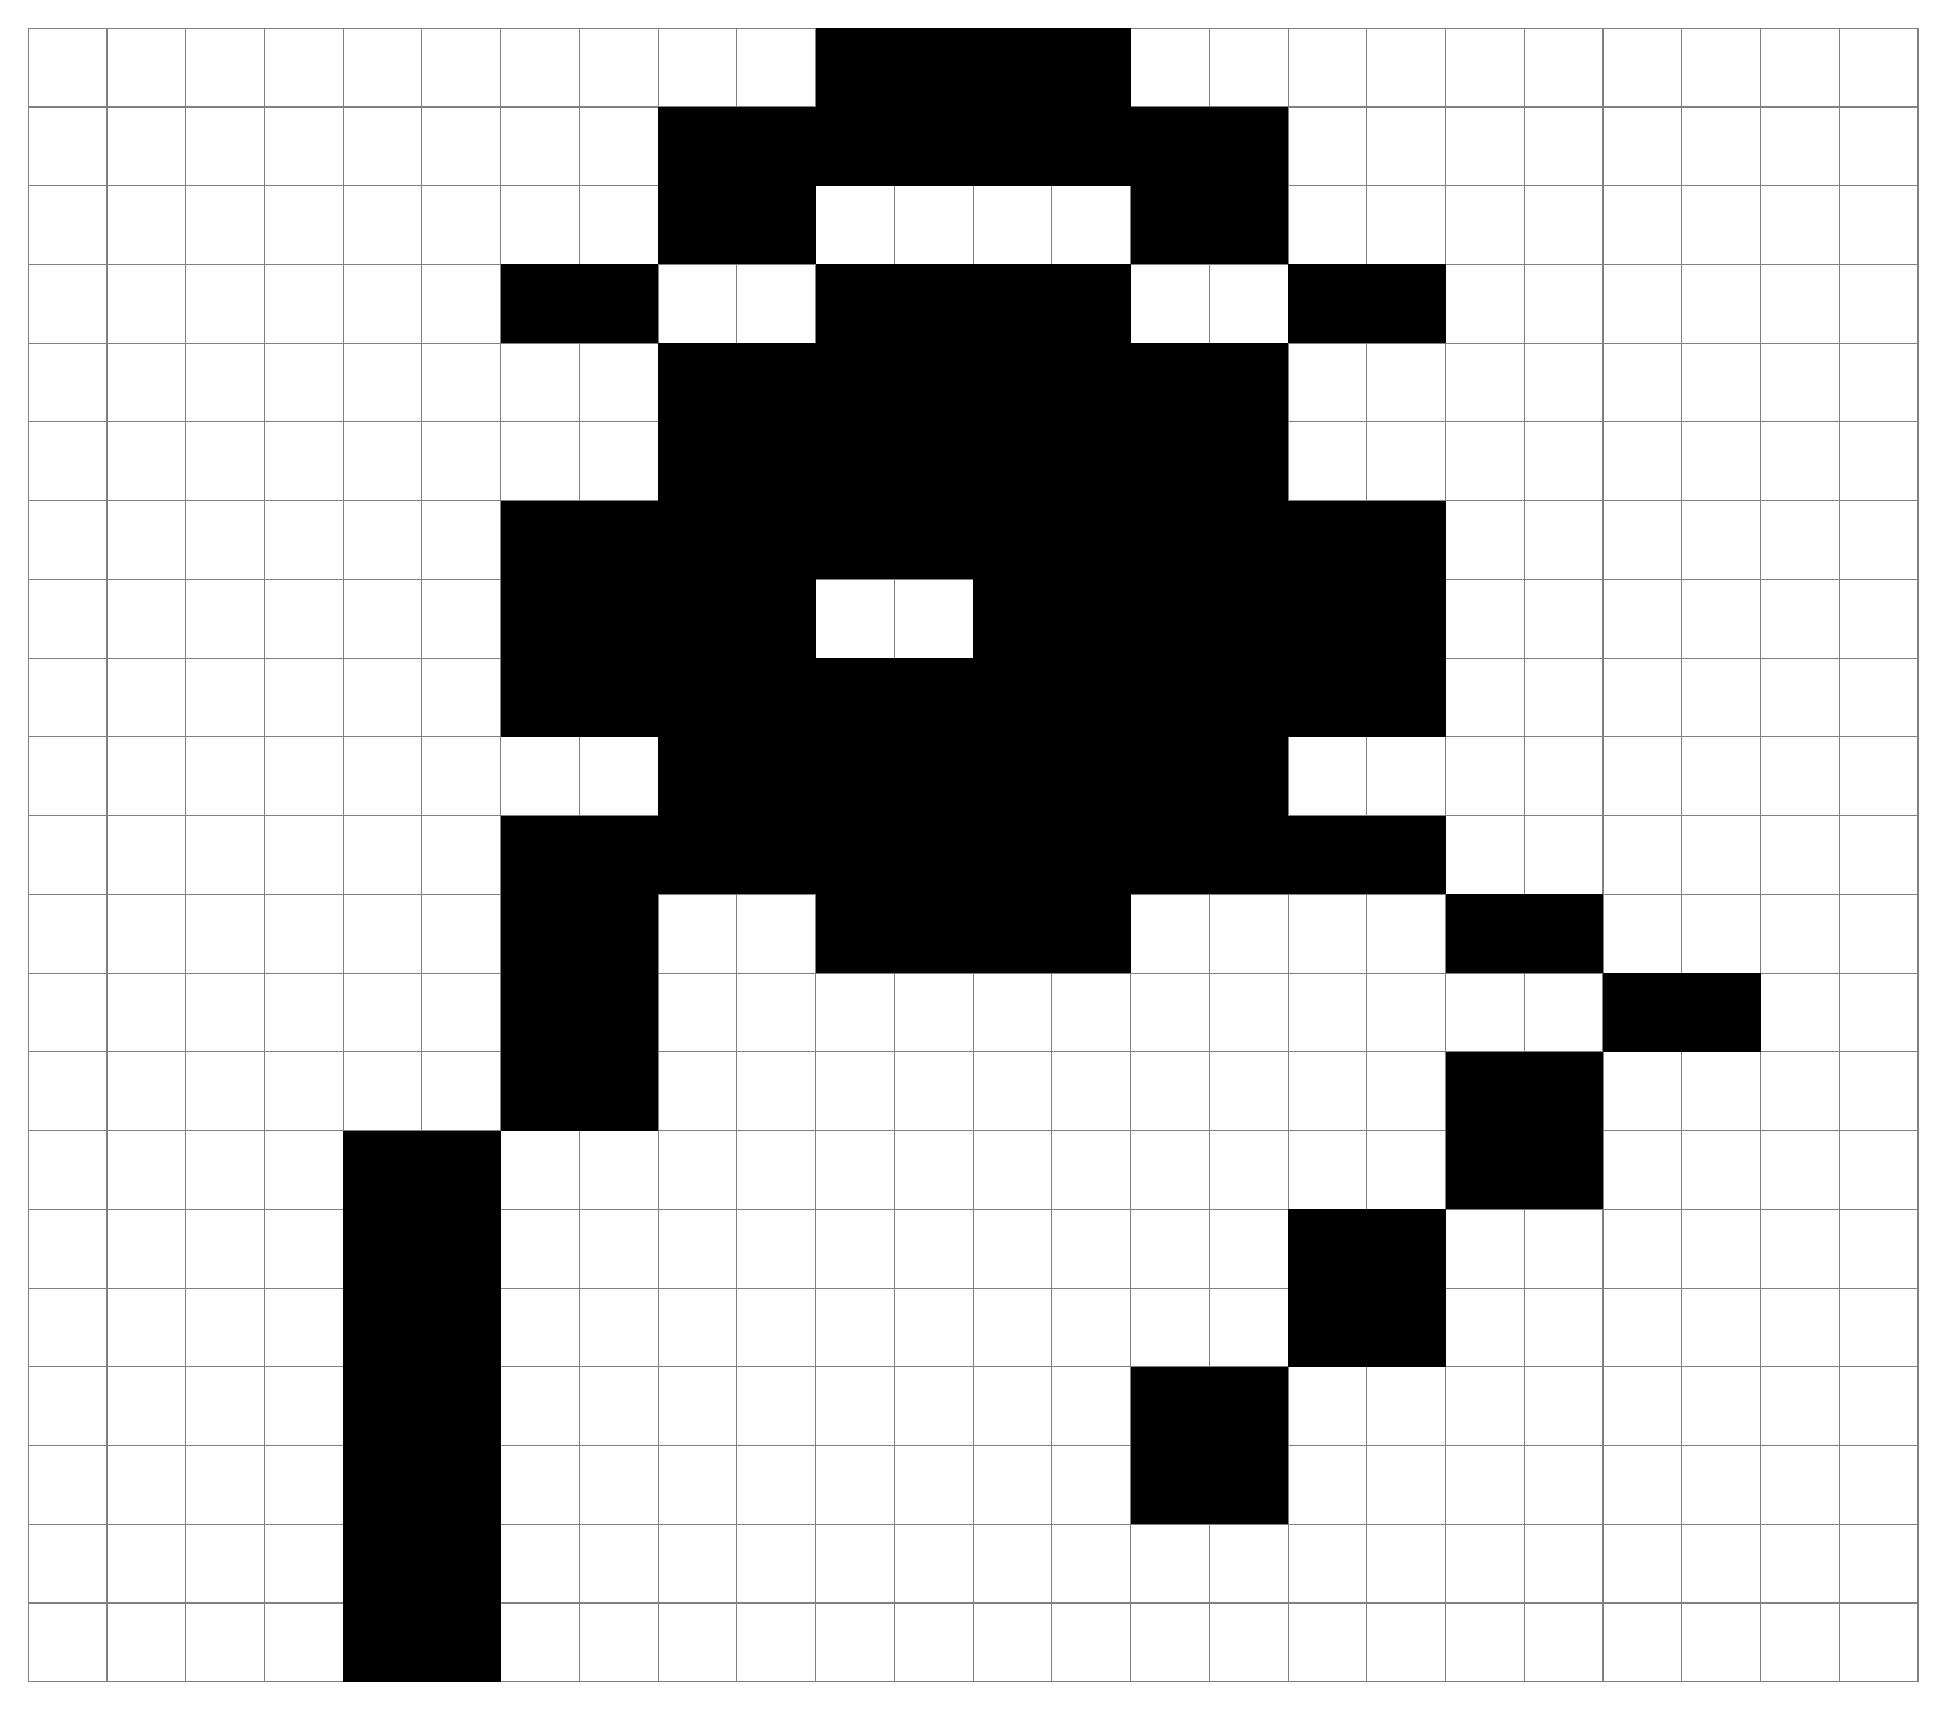
\begin{tikzpicture}

	\draw[step=1.0,gray,thin] (0,0) grid (24,21);
	\fill[\SPRITECOLOR] (10,20) rectangle ++ (1,1);
	\fill[\SPRITECOLOR] (11,20) rectangle ++ (1,1);
	\fill[\SPRITECOLOR] (12,20) rectangle ++ (1,1);
	\fill[\SPRITECOLOR] (13,20) rectangle ++ (1,1);
	\fill[\SPRITECOLOR] (8,19) rectangle ++ (1,1);
	\fill[\SPRITECOLOR] (9,19) rectangle ++ (1,1);
	\fill[\SPRITECOLOR] (10,19) rectangle ++ (1,1);
	\fill[\SPRITECOLOR] (11,19) rectangle ++ (1,1);
	\fill[\SPRITECOLOR] (12,19) rectangle ++ (1,1);
	\fill[\SPRITECOLOR] (13,19) rectangle ++ (1,1);
	\fill[\SPRITECOLOR] (14,19) rectangle ++ (1,1);
	\fill[\SPRITECOLOR] (15,19) rectangle ++ (1,1);
	\fill[\SPRITECOLOR] (8,18) rectangle ++ (1,1);
	\fill[\SPRITECOLOR] (9,18) rectangle ++ (1,1);
	\fill[\SPRITECOLOR] (14,18) rectangle ++ (1,1);
	\fill[\SPRITECOLOR] (15,18) rectangle ++ (1,1);
	\fill[\SPRITECOLOR] (6,17) rectangle ++ (1,1);
	\fill[\SPRITECOLOR] (7,17) rectangle ++ (1,1);
	\fill[\SPRITECOLOR] (10,17) rectangle ++ (1,1);
	\fill[\SPRITECOLOR] (11,17) rectangle ++ (1,1);
	\fill[\SPRITECOLOR] (12,17) rectangle ++ (1,1);
	\fill[\SPRITECOLOR] (13,17) rectangle ++ (1,1);
	\fill[\SPRITECOLOR] (16,17) rectangle ++ (1,1);
	\fill[\SPRITECOLOR] (17,17) rectangle ++ (1,1);
	\fill[\SPRITECOLOR] (8,16) rectangle ++ (1,1);
	\fill[\SPRITECOLOR] (9,16) rectangle ++ (1,1);
	\fill[\MULTICOLORTWO] (10,16) rectangle ++ (1,1);
	\fill[\MULTICOLORTWO] (11,16) rectangle ++ (1,1);
	\fill[\SPRITECOLOR] (12,16) rectangle ++ (1,1);
	\fill[\SPRITECOLOR] (13,16) rectangle ++ (1,1);
	\fill[\SPRITECOLOR] (14,16) rectangle ++ (1,1);
	\fill[\SPRITECOLOR] (15,16) rectangle ++ (1,1);
	\fill[\MULTICOLORTWO] (8,15) rectangle ++ (1,1);
	\fill[\MULTICOLORTWO] (9,15) rectangle ++ (1,1);
	\fill[\SPRITECOLOR] (10,15) rectangle ++ (1,1);
	\fill[\SPRITECOLOR] (11,15) rectangle ++ (1,1);
	\fill[\SPRITECOLOR] (12,15) rectangle ++ (1,1);
	\fill[\SPRITECOLOR] (13,15) rectangle ++ (1,1);
	\fill[\SPRITECOLOR] (14,15) rectangle ++ (1,1);
	\fill[\SPRITECOLOR] (15,15) rectangle ++ (1,1);
	\fill[\SPRITECOLOR] (6,14) rectangle ++ (1,1);
	\fill[\SPRITECOLOR] (7,14) rectangle ++ (1,1);
	\fill[\MULTICOLORTWO] (8,14) rectangle ++ (1,1);
	\fill[\MULTICOLORTWO] (9,14) rectangle ++ (1,1);
	\fill[\MULTICOLORTWO] (10,14) rectangle ++ (1,1);
	\fill[\MULTICOLORTWO] (11,14) rectangle ++ (1,1);
	\fill[\MULTICOLORTWO] (12,14) rectangle ++ (1,1);
	\fill[\MULTICOLORTWO] (13,14) rectangle ++ (1,1);
	\fill[\SPRITECOLOR] (14,14) rectangle ++ (1,1);
	\fill[\SPRITECOLOR] (15,14) rectangle ++ (1,1);
	\fill[\SPRITECOLOR] (16,14) rectangle ++ (1,1);
	\fill[\SPRITECOLOR] (17,14) rectangle ++ (1,1);
	\fill[\SPRITECOLOR] (6,13) rectangle ++ (1,1);
	\fill[\SPRITECOLOR] (7,13) rectangle ++ (1,1);
	\fill[\MULTICOLORTWO] (8,13) rectangle ++ (1,1);
	\fill[\MULTICOLORTWO] (9,13) rectangle ++ (1,1);
	\fill[\MULTICOLORTWO] (12,13) rectangle ++ (1,1);
	\fill[\MULTICOLORTWO] (13,13) rectangle ++ (1,1);
	\fill[\SPRITECOLOR] (14,13) rectangle ++ (1,1);
	\fill[\SPRITECOLOR] (15,13) rectangle ++ (1,1);
	\fill[\SPRITECOLOR] (16,13) rectangle ++ (1,1);
	\fill[\SPRITECOLOR] (17,13) rectangle ++ (1,1);
	\fill[\SPRITECOLOR] (6,12) rectangle ++ (1,1);
	\fill[\SPRITECOLOR] (7,12) rectangle ++ (1,1);
	\fill[\MULTICOLORTWO] (8,12) rectangle ++ (1,1);
	\fill[\MULTICOLORTWO] (9,12) rectangle ++ (1,1);
	\fill[\MULTICOLORTWO] (10,12) rectangle ++ (1,1);
	\fill[\MULTICOLORTWO] (11,12) rectangle ++ (1,1);
	\fill[\MULTICOLORTWO] (12,12) rectangle ++ (1,1);
	\fill[\MULTICOLORTWO] (13,12) rectangle ++ (1,1);
	\fill[\SPRITECOLOR] (14,12) rectangle ++ (1,1);
	\fill[\SPRITECOLOR] (15,12) rectangle ++ (1,1);
	\fill[\SPRITECOLOR] (16,12) rectangle ++ (1,1);
	\fill[\SPRITECOLOR] (17,12) rectangle ++ (1,1);
	\fill[\SPRITECOLOR] (8,11) rectangle ++ (1,1);
	\fill[\SPRITECOLOR] (9,11) rectangle ++ (1,1);
	\fill[\SPRITECOLOR] (10,11) rectangle ++ (1,1);
	\fill[\SPRITECOLOR] (11,11) rectangle ++ (1,1);
	\fill[\SPRITECOLOR] (12,11) rectangle ++ (1,1);
	\fill[\SPRITECOLOR] (13,11) rectangle ++ (1,1);
	\fill[\SPRITECOLOR] (14,11) rectangle ++ (1,1);
	\fill[\SPRITECOLOR] (15,11) rectangle ++ (1,1);
	\fill[\MULTICOLORONE] (6,10) rectangle ++ (1,1);
	\fill[\MULTICOLORONE] (7,10) rectangle ++ (1,1);
	\fill[\SPRITECOLOR] (8,10) rectangle ++ (1,1);
	\fill[\SPRITECOLOR] (9,10) rectangle ++ (1,1);
	\fill[\SPRITECOLOR] (10,10) rectangle ++ (1,1);
	\fill[\SPRITECOLOR] (11,10) rectangle ++ (1,1);
	\fill[\SPRITECOLOR] (12,10) rectangle ++ (1,1);
	\fill[\SPRITECOLOR] (13,10) rectangle ++ (1,1);
	\fill[\SPRITECOLOR] (14,10) rectangle ++ (1,1);
	\fill[\SPRITECOLOR] (15,10) rectangle ++ (1,1);
	\fill[\MULTICOLORONE] (16,10) rectangle ++ (1,1);
	\fill[\MULTICOLORONE] (17,10) rectangle ++ (1,1);
	\fill[\MULTICOLORONE] (6,9) rectangle ++ (1,1);
	\fill[\MULTICOLORONE] (7,9) rectangle ++ (1,1);
	\fill[\SPRITECOLOR] (10,9) rectangle ++ (1,1);
	\fill[\SPRITECOLOR] (11,9) rectangle ++ (1,1);
	\fill[\SPRITECOLOR] (12,9) rectangle ++ (1,1);
	\fill[\SPRITECOLOR] (13,9) rectangle ++ (1,1);
	\fill[\MULTICOLORONE] (18,9) rectangle ++ (1,1);
	\fill[\MULTICOLORONE] (19,9) rectangle ++ (1,1);
	\fill[\MULTICOLORONE] (6,8) rectangle ++ (1,1);
	\fill[\MULTICOLORONE] (7,8) rectangle ++ (1,1);
	\fill[\MULTICOLORTWO] (20,8) rectangle ++ (1,1);
	\fill[\MULTICOLORTWO] (21,8) rectangle ++ (1,1);
	\fill[\MULTICOLORONE] (6,7) rectangle ++ (1,1);
	\fill[\MULTICOLORONE] (7,7) rectangle ++ (1,1);
	\fill[\MULTICOLORONE] (18,7) rectangle ++ (1,1);
	\fill[\MULTICOLORONE] (19,7) rectangle ++ (1,1);
	\fill[\MULTICOLORTWO] (4,6) rectangle ++ (1,1);
	\fill[\MULTICOLORTWO] (5,6) rectangle ++ (1,1);
	\fill[\MULTICOLORONE] (18,6) rectangle ++ (1,1);
	\fill[\MULTICOLORONE] (19,6) rectangle ++ (1,1);
	\fill[\MULTICOLORONE] (4,5) rectangle ++ (1,1);
	\fill[\MULTICOLORONE] (5,5) rectangle ++ (1,1);
	\fill[\MULTICOLORONE] (16,5) rectangle ++ (1,1);
	\fill[\MULTICOLORONE] (17,5) rectangle ++ (1,1);
	\fill[\MULTICOLORONE] (4,4) rectangle ++ (1,1);
	\fill[\MULTICOLORONE] (5,4) rectangle ++ (1,1);
	\fill[\MULTICOLORONE] (16,4) rectangle ++ (1,1);
	\fill[\MULTICOLORONE] (17,4) rectangle ++ (1,1);
	\fill[\MULTICOLORONE] (4,3) rectangle ++ (1,1);
	\fill[\MULTICOLORONE] (5,3) rectangle ++ (1,1);
	\fill[\MULTICOLORONE] (14,3) rectangle ++ (1,1);
	\fill[\MULTICOLORONE] (15,3) rectangle ++ (1,1);
	\fill[\MULTICOLORONE] (4,2) rectangle ++ (1,1);
	\fill[\MULTICOLORONE] (5,2) rectangle ++ (1,1);
	\fill[\MULTICOLORONE] (14,2) rectangle ++ (1,1);
	\fill[\MULTICOLORONE] (15,2) rectangle ++ (1,1);
	\fill[\MULTICOLORONE] (4,1) rectangle ++ (1,1);
	\fill[\MULTICOLORONE] (5,1) rectangle ++ (1,1);
	\fill[\MULTICOLORONE] (4,0) rectangle ++ (1,1);
	\fill[\MULTICOLORONE] (5,0) rectangle ++ (1,1);

      \end{tikzpicture}
    \end{adjustbox}
  }\caption{LAND\_GILBY3}
\end{figure}

	\end{subfigure}
} & 
\makecell[l]{
	\begin{subfigure}{0.3\textwidth}
    \def\MULTICOLORONE{gray}
    \def\MULTICOLORTWO{white}
    \def\SPRITECOLOR{yellow}
		
\begin{figure}[H]
  {
    \setlength{\tabcolsep}{3.0pt}
    \setlength\cmidrulewidth{\heavyrulewidth} % Make cmidrule = 
    \begin{adjustbox}{width=3cm,center}
      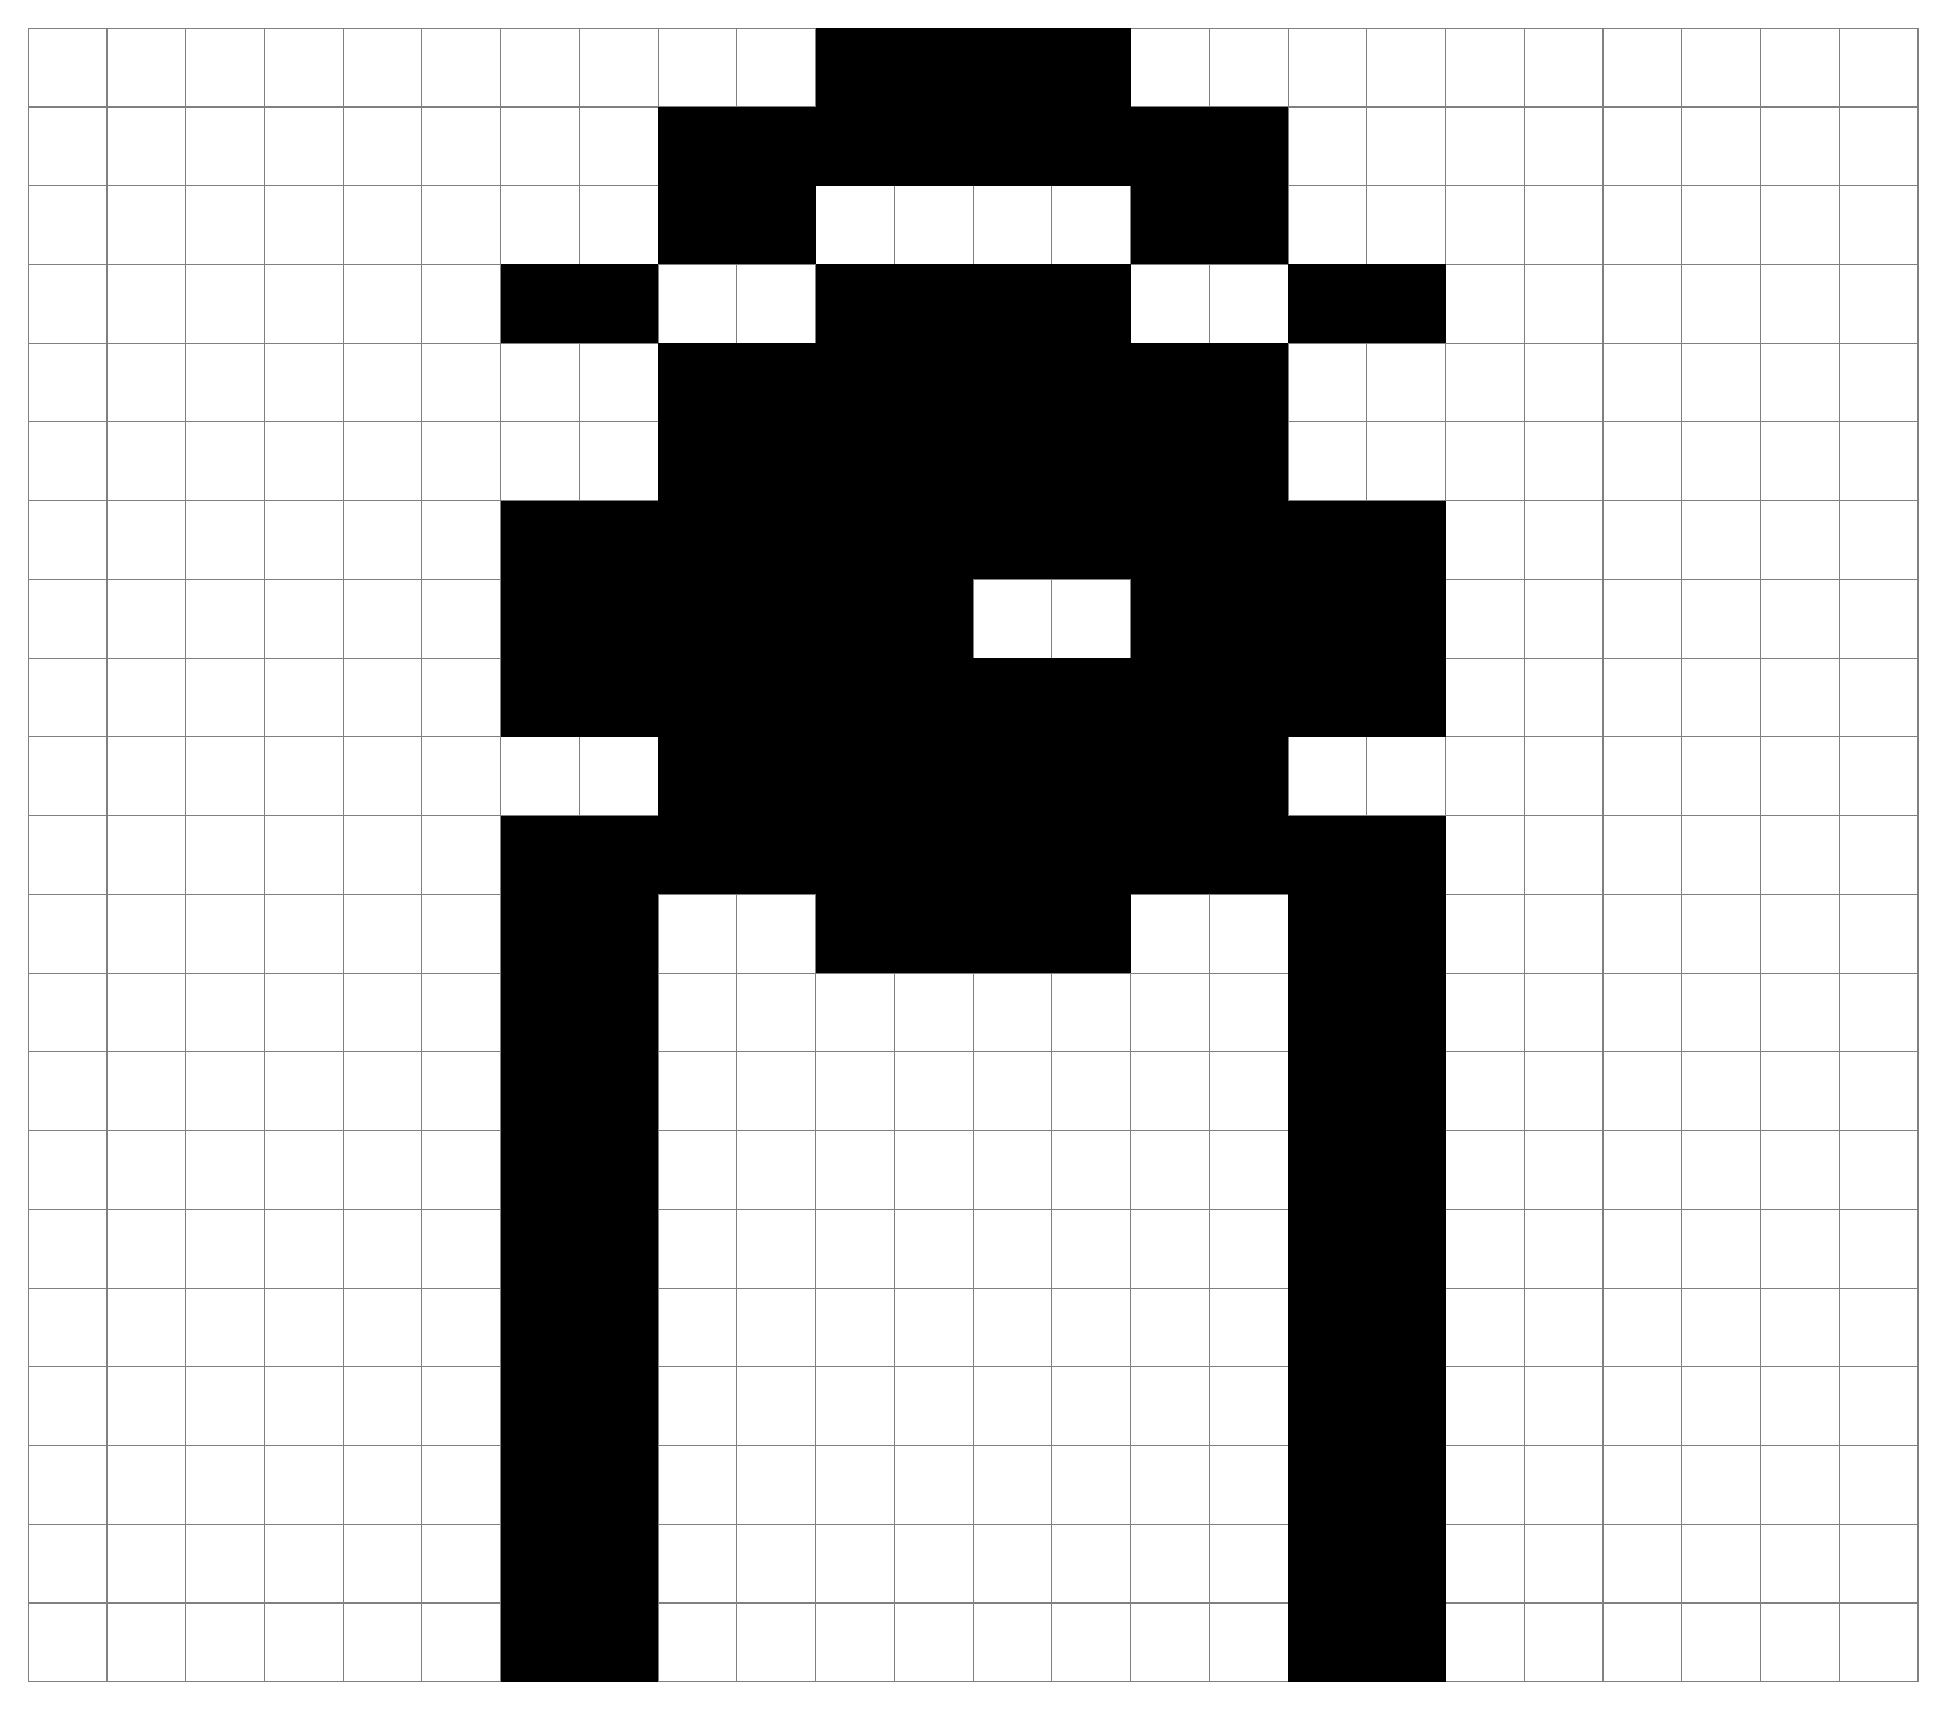
\begin{tikzpicture}

	\draw[step=1.0,gray,thin] (0,0) grid (24,21);
	\fill[\SPRITECOLOR] (10,20) rectangle ++ (1,1);
	\fill[\SPRITECOLOR] (11,20) rectangle ++ (1,1);
	\fill[\SPRITECOLOR] (12,20) rectangle ++ (1,1);
	\fill[\SPRITECOLOR] (13,20) rectangle ++ (1,1);
	\fill[\SPRITECOLOR] (8,19) rectangle ++ (1,1);
	\fill[\SPRITECOLOR] (9,19) rectangle ++ (1,1);
	\fill[\SPRITECOLOR] (10,19) rectangle ++ (1,1);
	\fill[\SPRITECOLOR] (11,19) rectangle ++ (1,1);
	\fill[\SPRITECOLOR] (12,19) rectangle ++ (1,1);
	\fill[\SPRITECOLOR] (13,19) rectangle ++ (1,1);
	\fill[\SPRITECOLOR] (14,19) rectangle ++ (1,1);
	\fill[\SPRITECOLOR] (15,19) rectangle ++ (1,1);
	\fill[\SPRITECOLOR] (8,18) rectangle ++ (1,1);
	\fill[\SPRITECOLOR] (9,18) rectangle ++ (1,1);
	\fill[\SPRITECOLOR] (14,18) rectangle ++ (1,1);
	\fill[\SPRITECOLOR] (15,18) rectangle ++ (1,1);
	\fill[\SPRITECOLOR] (6,17) rectangle ++ (1,1);
	\fill[\SPRITECOLOR] (7,17) rectangle ++ (1,1);
	\fill[\SPRITECOLOR] (10,17) rectangle ++ (1,1);
	\fill[\SPRITECOLOR] (11,17) rectangle ++ (1,1);
	\fill[\SPRITECOLOR] (12,17) rectangle ++ (1,1);
	\fill[\SPRITECOLOR] (13,17) rectangle ++ (1,1);
	\fill[\SPRITECOLOR] (16,17) rectangle ++ (1,1);
	\fill[\SPRITECOLOR] (17,17) rectangle ++ (1,1);
	\fill[\SPRITECOLOR] (8,16) rectangle ++ (1,1);
	\fill[\SPRITECOLOR] (9,16) rectangle ++ (1,1);
	\fill[\MULTICOLORTWO] (10,16) rectangle ++ (1,1);
	\fill[\MULTICOLORTWO] (11,16) rectangle ++ (1,1);
	\fill[\SPRITECOLOR] (12,16) rectangle ++ (1,1);
	\fill[\SPRITECOLOR] (13,16) rectangle ++ (1,1);
	\fill[\SPRITECOLOR] (14,16) rectangle ++ (1,1);
	\fill[\SPRITECOLOR] (15,16) rectangle ++ (1,1);
	\fill[\MULTICOLORTWO] (8,15) rectangle ++ (1,1);
	\fill[\MULTICOLORTWO] (9,15) rectangle ++ (1,1);
	\fill[\SPRITECOLOR] (10,15) rectangle ++ (1,1);
	\fill[\SPRITECOLOR] (11,15) rectangle ++ (1,1);
	\fill[\SPRITECOLOR] (12,15) rectangle ++ (1,1);
	\fill[\SPRITECOLOR] (13,15) rectangle ++ (1,1);
	\fill[\SPRITECOLOR] (14,15) rectangle ++ (1,1);
	\fill[\SPRITECOLOR] (15,15) rectangle ++ (1,1);
	\fill[\SPRITECOLOR] (6,14) rectangle ++ (1,1);
	\fill[\SPRITECOLOR] (7,14) rectangle ++ (1,1);
	\fill[\SPRITECOLOR] (8,14) rectangle ++ (1,1);
	\fill[\SPRITECOLOR] (9,14) rectangle ++ (1,1);
	\fill[\MULTICOLORTWO] (10,14) rectangle ++ (1,1);
	\fill[\MULTICOLORTWO] (11,14) rectangle ++ (1,1);
	\fill[\MULTICOLORTWO] (12,14) rectangle ++ (1,1);
	\fill[\MULTICOLORTWO] (13,14) rectangle ++ (1,1);
	\fill[\MULTICOLORTWO] (14,14) rectangle ++ (1,1);
	\fill[\MULTICOLORTWO] (15,14) rectangle ++ (1,1);
	\fill[\SPRITECOLOR] (16,14) rectangle ++ (1,1);
	\fill[\SPRITECOLOR] (17,14) rectangle ++ (1,1);
	\fill[\SPRITECOLOR] (6,13) rectangle ++ (1,1);
	\fill[\SPRITECOLOR] (7,13) rectangle ++ (1,1);
	\fill[\SPRITECOLOR] (8,13) rectangle ++ (1,1);
	\fill[\SPRITECOLOR] (9,13) rectangle ++ (1,1);
	\fill[\MULTICOLORTWO] (10,13) rectangle ++ (1,1);
	\fill[\MULTICOLORTWO] (11,13) rectangle ++ (1,1);
	\fill[\MULTICOLORTWO] (14,13) rectangle ++ (1,1);
	\fill[\MULTICOLORTWO] (15,13) rectangle ++ (1,1);
	\fill[\SPRITECOLOR] (16,13) rectangle ++ (1,1);
	\fill[\SPRITECOLOR] (17,13) rectangle ++ (1,1);
	\fill[\SPRITECOLOR] (6,12) rectangle ++ (1,1);
	\fill[\SPRITECOLOR] (7,12) rectangle ++ (1,1);
	\fill[\SPRITECOLOR] (8,12) rectangle ++ (1,1);
	\fill[\SPRITECOLOR] (9,12) rectangle ++ (1,1);
	\fill[\MULTICOLORTWO] (10,12) rectangle ++ (1,1);
	\fill[\MULTICOLORTWO] (11,12) rectangle ++ (1,1);
	\fill[\MULTICOLORTWO] (12,12) rectangle ++ (1,1);
	\fill[\MULTICOLORTWO] (13,12) rectangle ++ (1,1);
	\fill[\MULTICOLORTWO] (14,12) rectangle ++ (1,1);
	\fill[\MULTICOLORTWO] (15,12) rectangle ++ (1,1);
	\fill[\SPRITECOLOR] (16,12) rectangle ++ (1,1);
	\fill[\SPRITECOLOR] (17,12) rectangle ++ (1,1);
	\fill[\SPRITECOLOR] (8,11) rectangle ++ (1,1);
	\fill[\SPRITECOLOR] (9,11) rectangle ++ (1,1);
	\fill[\SPRITECOLOR] (10,11) rectangle ++ (1,1);
	\fill[\SPRITECOLOR] (11,11) rectangle ++ (1,1);
	\fill[\SPRITECOLOR] (12,11) rectangle ++ (1,1);
	\fill[\SPRITECOLOR] (13,11) rectangle ++ (1,1);
	\fill[\SPRITECOLOR] (14,11) rectangle ++ (1,1);
	\fill[\SPRITECOLOR] (15,11) rectangle ++ (1,1);
	\fill[\MULTICOLORONE] (6,10) rectangle ++ (1,1);
	\fill[\MULTICOLORONE] (7,10) rectangle ++ (1,1);
	\fill[\SPRITECOLOR] (8,10) rectangle ++ (1,1);
	\fill[\SPRITECOLOR] (9,10) rectangle ++ (1,1);
	\fill[\SPRITECOLOR] (10,10) rectangle ++ (1,1);
	\fill[\SPRITECOLOR] (11,10) rectangle ++ (1,1);
	\fill[\SPRITECOLOR] (12,10) rectangle ++ (1,1);
	\fill[\SPRITECOLOR] (13,10) rectangle ++ (1,1);
	\fill[\SPRITECOLOR] (14,10) rectangle ++ (1,1);
	\fill[\SPRITECOLOR] (15,10) rectangle ++ (1,1);
	\fill[\MULTICOLORONE] (16,10) rectangle ++ (1,1);
	\fill[\MULTICOLORONE] (17,10) rectangle ++ (1,1);
	\fill[\MULTICOLORONE] (6,9) rectangle ++ (1,1);
	\fill[\MULTICOLORONE] (7,9) rectangle ++ (1,1);
	\fill[\SPRITECOLOR] (10,9) rectangle ++ (1,1);
	\fill[\SPRITECOLOR] (11,9) rectangle ++ (1,1);
	\fill[\SPRITECOLOR] (12,9) rectangle ++ (1,1);
	\fill[\SPRITECOLOR] (13,9) rectangle ++ (1,1);
	\fill[\MULTICOLORONE] (16,9) rectangle ++ (1,1);
	\fill[\MULTICOLORONE] (17,9) rectangle ++ (1,1);
	\fill[\MULTICOLORONE] (6,8) rectangle ++ (1,1);
	\fill[\MULTICOLORONE] (7,8) rectangle ++ (1,1);
	\fill[\MULTICOLORONE] (16,8) rectangle ++ (1,1);
	\fill[\MULTICOLORONE] (17,8) rectangle ++ (1,1);
	\fill[\MULTICOLORONE] (6,7) rectangle ++ (1,1);
	\fill[\MULTICOLORONE] (7,7) rectangle ++ (1,1);
	\fill[\MULTICOLORONE] (16,7) rectangle ++ (1,1);
	\fill[\MULTICOLORONE] (17,7) rectangle ++ (1,1);
	\fill[\MULTICOLORTWO] (6,6) rectangle ++ (1,1);
	\fill[\MULTICOLORTWO] (7,6) rectangle ++ (1,1);
	\fill[\MULTICOLORTWO] (16,6) rectangle ++ (1,1);
	\fill[\MULTICOLORTWO] (17,6) rectangle ++ (1,1);
	\fill[\MULTICOLORONE] (6,5) rectangle ++ (1,1);
	\fill[\MULTICOLORONE] (7,5) rectangle ++ (1,1);
	\fill[\MULTICOLORONE] (16,5) rectangle ++ (1,1);
	\fill[\MULTICOLORONE] (17,5) rectangle ++ (1,1);
	\fill[\MULTICOLORONE] (6,4) rectangle ++ (1,1);
	\fill[\MULTICOLORONE] (7,4) rectangle ++ (1,1);
	\fill[\MULTICOLORONE] (16,4) rectangle ++ (1,1);
	\fill[\MULTICOLORONE] (17,4) rectangle ++ (1,1);
	\fill[\MULTICOLORONE] (6,3) rectangle ++ (1,1);
	\fill[\MULTICOLORONE] (7,3) rectangle ++ (1,1);
	\fill[\MULTICOLORONE] (16,3) rectangle ++ (1,1);
	\fill[\MULTICOLORONE] (17,3) rectangle ++ (1,1);
	\fill[\MULTICOLORONE] (6,2) rectangle ++ (1,1);
	\fill[\MULTICOLORONE] (7,2) rectangle ++ (1,1);
	\fill[\MULTICOLORONE] (16,2) rectangle ++ (1,1);
	\fill[\MULTICOLORONE] (17,2) rectangle ++ (1,1);
	\fill[\MULTICOLORONE] (6,1) rectangle ++ (1,1);
	\fill[\MULTICOLORONE] (7,1) rectangle ++ (1,1);
	\fill[\MULTICOLORONE] (16,1) rectangle ++ (1,1);
	\fill[\MULTICOLORONE] (17,1) rectangle ++ (1,1);
	\fill[\MULTICOLORONE] (6,0) rectangle ++ (1,1);
	\fill[\MULTICOLORONE] (7,0) rectangle ++ (1,1);
	\fill[\MULTICOLORONE] (16,0) rectangle ++ (1,1);
	\fill[\MULTICOLORONE] (17,0) rectangle ++ (1,1);

      \end{tikzpicture}
    \end{adjustbox}
  }\caption{LAND\_GILBY4}
\end{figure}

	\end{subfigure}
} & 
\makecell[l]{
	\begin{subfigure}{0.3\textwidth}
    \def\MULTICOLORONE{gray}
    \def\MULTICOLORTWO{white}
    \def\SPRITECOLOR{green}
		
\begin{figure}[H]
  {
    \setlength{\tabcolsep}{3.0pt}
    \setlength\cmidrulewidth{\heavyrulewidth} % Make cmidrule = 
    \begin{adjustbox}{width=3cm,center}
      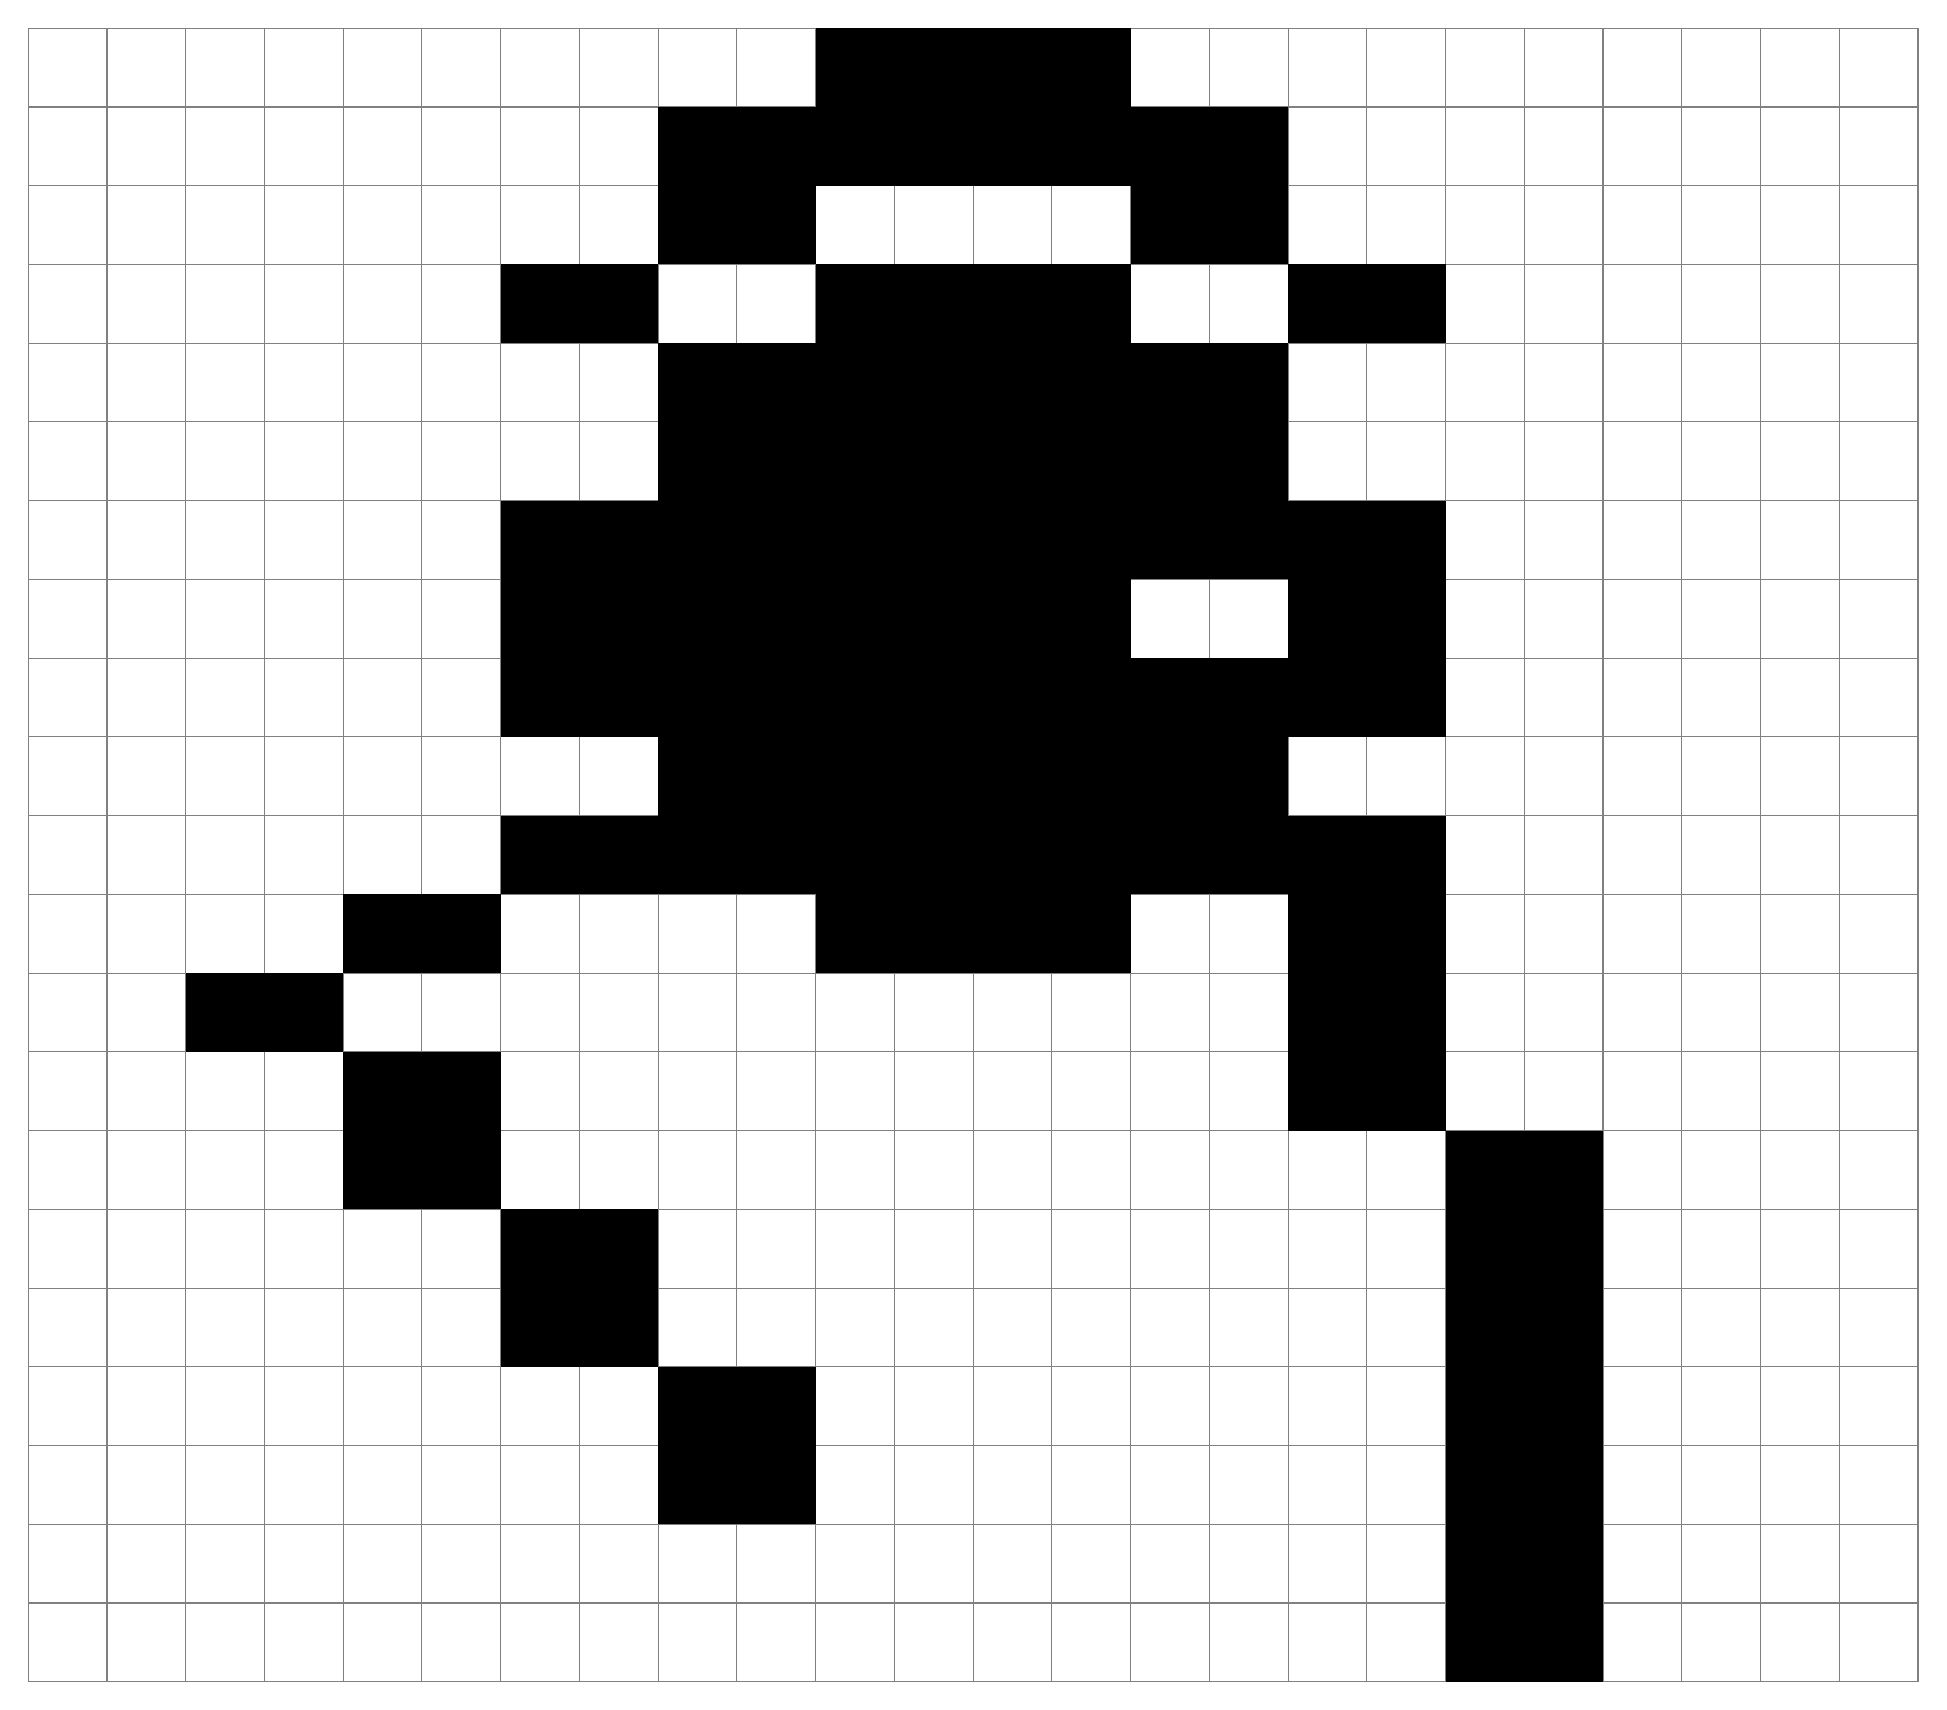
\begin{tikzpicture}

	\draw[step=1.0,gray,thin] (0,0) grid (24,21);
	\fill[\SPRITECOLOR] (10,20) rectangle ++ (1,1);
	\fill[\SPRITECOLOR] (11,20) rectangle ++ (1,1);
	\fill[\SPRITECOLOR] (12,20) rectangle ++ (1,1);
	\fill[\SPRITECOLOR] (13,20) rectangle ++ (1,1);
	\fill[\SPRITECOLOR] (8,19) rectangle ++ (1,1);
	\fill[\SPRITECOLOR] (9,19) rectangle ++ (1,1);
	\fill[\SPRITECOLOR] (10,19) rectangle ++ (1,1);
	\fill[\SPRITECOLOR] (11,19) rectangle ++ (1,1);
	\fill[\SPRITECOLOR] (12,19) rectangle ++ (1,1);
	\fill[\SPRITECOLOR] (13,19) rectangle ++ (1,1);
	\fill[\SPRITECOLOR] (14,19) rectangle ++ (1,1);
	\fill[\SPRITECOLOR] (15,19) rectangle ++ (1,1);
	\fill[\SPRITECOLOR] (8,18) rectangle ++ (1,1);
	\fill[\SPRITECOLOR] (9,18) rectangle ++ (1,1);
	\fill[\SPRITECOLOR] (14,18) rectangle ++ (1,1);
	\fill[\SPRITECOLOR] (15,18) rectangle ++ (1,1);
	\fill[\SPRITECOLOR] (6,17) rectangle ++ (1,1);
	\fill[\SPRITECOLOR] (7,17) rectangle ++ (1,1);
	\fill[\SPRITECOLOR] (10,17) rectangle ++ (1,1);
	\fill[\SPRITECOLOR] (11,17) rectangle ++ (1,1);
	\fill[\SPRITECOLOR] (12,17) rectangle ++ (1,1);
	\fill[\SPRITECOLOR] (13,17) rectangle ++ (1,1);
	\fill[\SPRITECOLOR] (16,17) rectangle ++ (1,1);
	\fill[\SPRITECOLOR] (17,17) rectangle ++ (1,1);
	\fill[\SPRITECOLOR] (8,16) rectangle ++ (1,1);
	\fill[\SPRITECOLOR] (9,16) rectangle ++ (1,1);
	\fill[\MULTICOLORTWO] (10,16) rectangle ++ (1,1);
	\fill[\MULTICOLORTWO] (11,16) rectangle ++ (1,1);
	\fill[\SPRITECOLOR] (12,16) rectangle ++ (1,1);
	\fill[\SPRITECOLOR] (13,16) rectangle ++ (1,1);
	\fill[\SPRITECOLOR] (14,16) rectangle ++ (1,1);
	\fill[\SPRITECOLOR] (15,16) rectangle ++ (1,1);
	\fill[\MULTICOLORTWO] (8,15) rectangle ++ (1,1);
	\fill[\MULTICOLORTWO] (9,15) rectangle ++ (1,1);
	\fill[\SPRITECOLOR] (10,15) rectangle ++ (1,1);
	\fill[\SPRITECOLOR] (11,15) rectangle ++ (1,1);
	\fill[\SPRITECOLOR] (12,15) rectangle ++ (1,1);
	\fill[\SPRITECOLOR] (13,15) rectangle ++ (1,1);
	\fill[\SPRITECOLOR] (14,15) rectangle ++ (1,1);
	\fill[\SPRITECOLOR] (15,15) rectangle ++ (1,1);
	\fill[\SPRITECOLOR] (6,14) rectangle ++ (1,1);
	\fill[\SPRITECOLOR] (7,14) rectangle ++ (1,1);
	\fill[\SPRITECOLOR] (8,14) rectangle ++ (1,1);
	\fill[\SPRITECOLOR] (9,14) rectangle ++ (1,1);
	\fill[\SPRITECOLOR] (10,14) rectangle ++ (1,1);
	\fill[\SPRITECOLOR] (11,14) rectangle ++ (1,1);
	\fill[\MULTICOLORTWO] (12,14) rectangle ++ (1,1);
	\fill[\MULTICOLORTWO] (13,14) rectangle ++ (1,1);
	\fill[\MULTICOLORTWO] (14,14) rectangle ++ (1,1);
	\fill[\MULTICOLORTWO] (15,14) rectangle ++ (1,1);
	\fill[\MULTICOLORTWO] (16,14) rectangle ++ (1,1);
	\fill[\MULTICOLORTWO] (17,14) rectangle ++ (1,1);
	\fill[\SPRITECOLOR] (6,13) rectangle ++ (1,1);
	\fill[\SPRITECOLOR] (7,13) rectangle ++ (1,1);
	\fill[\SPRITECOLOR] (8,13) rectangle ++ (1,1);
	\fill[\SPRITECOLOR] (9,13) rectangle ++ (1,1);
	\fill[\SPRITECOLOR] (10,13) rectangle ++ (1,1);
	\fill[\SPRITECOLOR] (11,13) rectangle ++ (1,1);
	\fill[\MULTICOLORTWO] (12,13) rectangle ++ (1,1);
	\fill[\MULTICOLORTWO] (13,13) rectangle ++ (1,1);
	\fill[\MULTICOLORTWO] (16,13) rectangle ++ (1,1);
	\fill[\MULTICOLORTWO] (17,13) rectangle ++ (1,1);
	\fill[\SPRITECOLOR] (6,12) rectangle ++ (1,1);
	\fill[\SPRITECOLOR] (7,12) rectangle ++ (1,1);
	\fill[\SPRITECOLOR] (8,12) rectangle ++ (1,1);
	\fill[\SPRITECOLOR] (9,12) rectangle ++ (1,1);
	\fill[\SPRITECOLOR] (10,12) rectangle ++ (1,1);
	\fill[\SPRITECOLOR] (11,12) rectangle ++ (1,1);
	\fill[\MULTICOLORTWO] (12,12) rectangle ++ (1,1);
	\fill[\MULTICOLORTWO] (13,12) rectangle ++ (1,1);
	\fill[\MULTICOLORTWO] (14,12) rectangle ++ (1,1);
	\fill[\MULTICOLORTWO] (15,12) rectangle ++ (1,1);
	\fill[\MULTICOLORTWO] (16,12) rectangle ++ (1,1);
	\fill[\MULTICOLORTWO] (17,12) rectangle ++ (1,1);
	\fill[\SPRITECOLOR] (8,11) rectangle ++ (1,1);
	\fill[\SPRITECOLOR] (9,11) rectangle ++ (1,1);
	\fill[\SPRITECOLOR] (10,11) rectangle ++ (1,1);
	\fill[\SPRITECOLOR] (11,11) rectangle ++ (1,1);
	\fill[\SPRITECOLOR] (12,11) rectangle ++ (1,1);
	\fill[\SPRITECOLOR] (13,11) rectangle ++ (1,1);
	\fill[\SPRITECOLOR] (14,11) rectangle ++ (1,1);
	\fill[\SPRITECOLOR] (15,11) rectangle ++ (1,1);
	\fill[\MULTICOLORONE] (6,10) rectangle ++ (1,1);
	\fill[\MULTICOLORONE] (7,10) rectangle ++ (1,1);
	\fill[\SPRITECOLOR] (8,10) rectangle ++ (1,1);
	\fill[\SPRITECOLOR] (9,10) rectangle ++ (1,1);
	\fill[\SPRITECOLOR] (10,10) rectangle ++ (1,1);
	\fill[\SPRITECOLOR] (11,10) rectangle ++ (1,1);
	\fill[\SPRITECOLOR] (12,10) rectangle ++ (1,1);
	\fill[\SPRITECOLOR] (13,10) rectangle ++ (1,1);
	\fill[\SPRITECOLOR] (14,10) rectangle ++ (1,1);
	\fill[\SPRITECOLOR] (15,10) rectangle ++ (1,1);
	\fill[\MULTICOLORONE] (16,10) rectangle ++ (1,1);
	\fill[\MULTICOLORONE] (17,10) rectangle ++ (1,1);
	\fill[\MULTICOLORONE] (4,9) rectangle ++ (1,1);
	\fill[\MULTICOLORONE] (5,9) rectangle ++ (1,1);
	\fill[\SPRITECOLOR] (10,9) rectangle ++ (1,1);
	\fill[\SPRITECOLOR] (11,9) rectangle ++ (1,1);
	\fill[\SPRITECOLOR] (12,9) rectangle ++ (1,1);
	\fill[\SPRITECOLOR] (13,9) rectangle ++ (1,1);
	\fill[\MULTICOLORONE] (16,9) rectangle ++ (1,1);
	\fill[\MULTICOLORONE] (17,9) rectangle ++ (1,1);
	\fill[\MULTICOLORTWO] (2,8) rectangle ++ (1,1);
	\fill[\MULTICOLORTWO] (3,8) rectangle ++ (1,1);
	\fill[\MULTICOLORONE] (16,8) rectangle ++ (1,1);
	\fill[\MULTICOLORONE] (17,8) rectangle ++ (1,1);
	\fill[\MULTICOLORONE] (4,7) rectangle ++ (1,1);
	\fill[\MULTICOLORONE] (5,7) rectangle ++ (1,1);
	\fill[\MULTICOLORONE] (16,7) rectangle ++ (1,1);
	\fill[\MULTICOLORONE] (17,7) rectangle ++ (1,1);
	\fill[\MULTICOLORONE] (4,6) rectangle ++ (1,1);
	\fill[\MULTICOLORONE] (5,6) rectangle ++ (1,1);
	\fill[\MULTICOLORTWO] (18,6) rectangle ++ (1,1);
	\fill[\MULTICOLORTWO] (19,6) rectangle ++ (1,1);
	\fill[\MULTICOLORONE] (6,5) rectangle ++ (1,1);
	\fill[\MULTICOLORONE] (7,5) rectangle ++ (1,1);
	\fill[\MULTICOLORONE] (18,5) rectangle ++ (1,1);
	\fill[\MULTICOLORONE] (19,5) rectangle ++ (1,1);
	\fill[\MULTICOLORONE] (6,4) rectangle ++ (1,1);
	\fill[\MULTICOLORONE] (7,4) rectangle ++ (1,1);
	\fill[\MULTICOLORONE] (18,4) rectangle ++ (1,1);
	\fill[\MULTICOLORONE] (19,4) rectangle ++ (1,1);
	\fill[\MULTICOLORONE] (8,3) rectangle ++ (1,1);
	\fill[\MULTICOLORONE] (9,3) rectangle ++ (1,1);
	\fill[\MULTICOLORONE] (18,3) rectangle ++ (1,1);
	\fill[\MULTICOLORONE] (19,3) rectangle ++ (1,1);
	\fill[\MULTICOLORONE] (8,2) rectangle ++ (1,1);
	\fill[\MULTICOLORONE] (9,2) rectangle ++ (1,1);
	\fill[\MULTICOLORONE] (18,2) rectangle ++ (1,1);
	\fill[\MULTICOLORONE] (19,2) rectangle ++ (1,1);
	\fill[\MULTICOLORONE] (18,1) rectangle ++ (1,1);
	\fill[\MULTICOLORONE] (19,1) rectangle ++ (1,1);
	\fill[\MULTICOLORONE] (18,0) rectangle ++ (1,1);
	\fill[\MULTICOLORONE] (19,0) rectangle ++ (1,1);

      \end{tikzpicture}
    \end{adjustbox}
  }\caption{LAND\_GILBY5}
\end{figure}

	\end{subfigure}
} & 
\makecell[l]{
	\begin{subfigure}{0.3\textwidth}
    \def\MULTICOLORONE{gray}
    \def\MULTICOLORTWO{white}
    \def\SPRITECOLOR{lightblue}
		
\begin{figure}[H]
  {
    \setlength{\tabcolsep}{3.0pt}
    \setlength\cmidrulewidth{\heavyrulewidth} % Make cmidrule = 
    \begin{adjustbox}{width=3cm,center}
      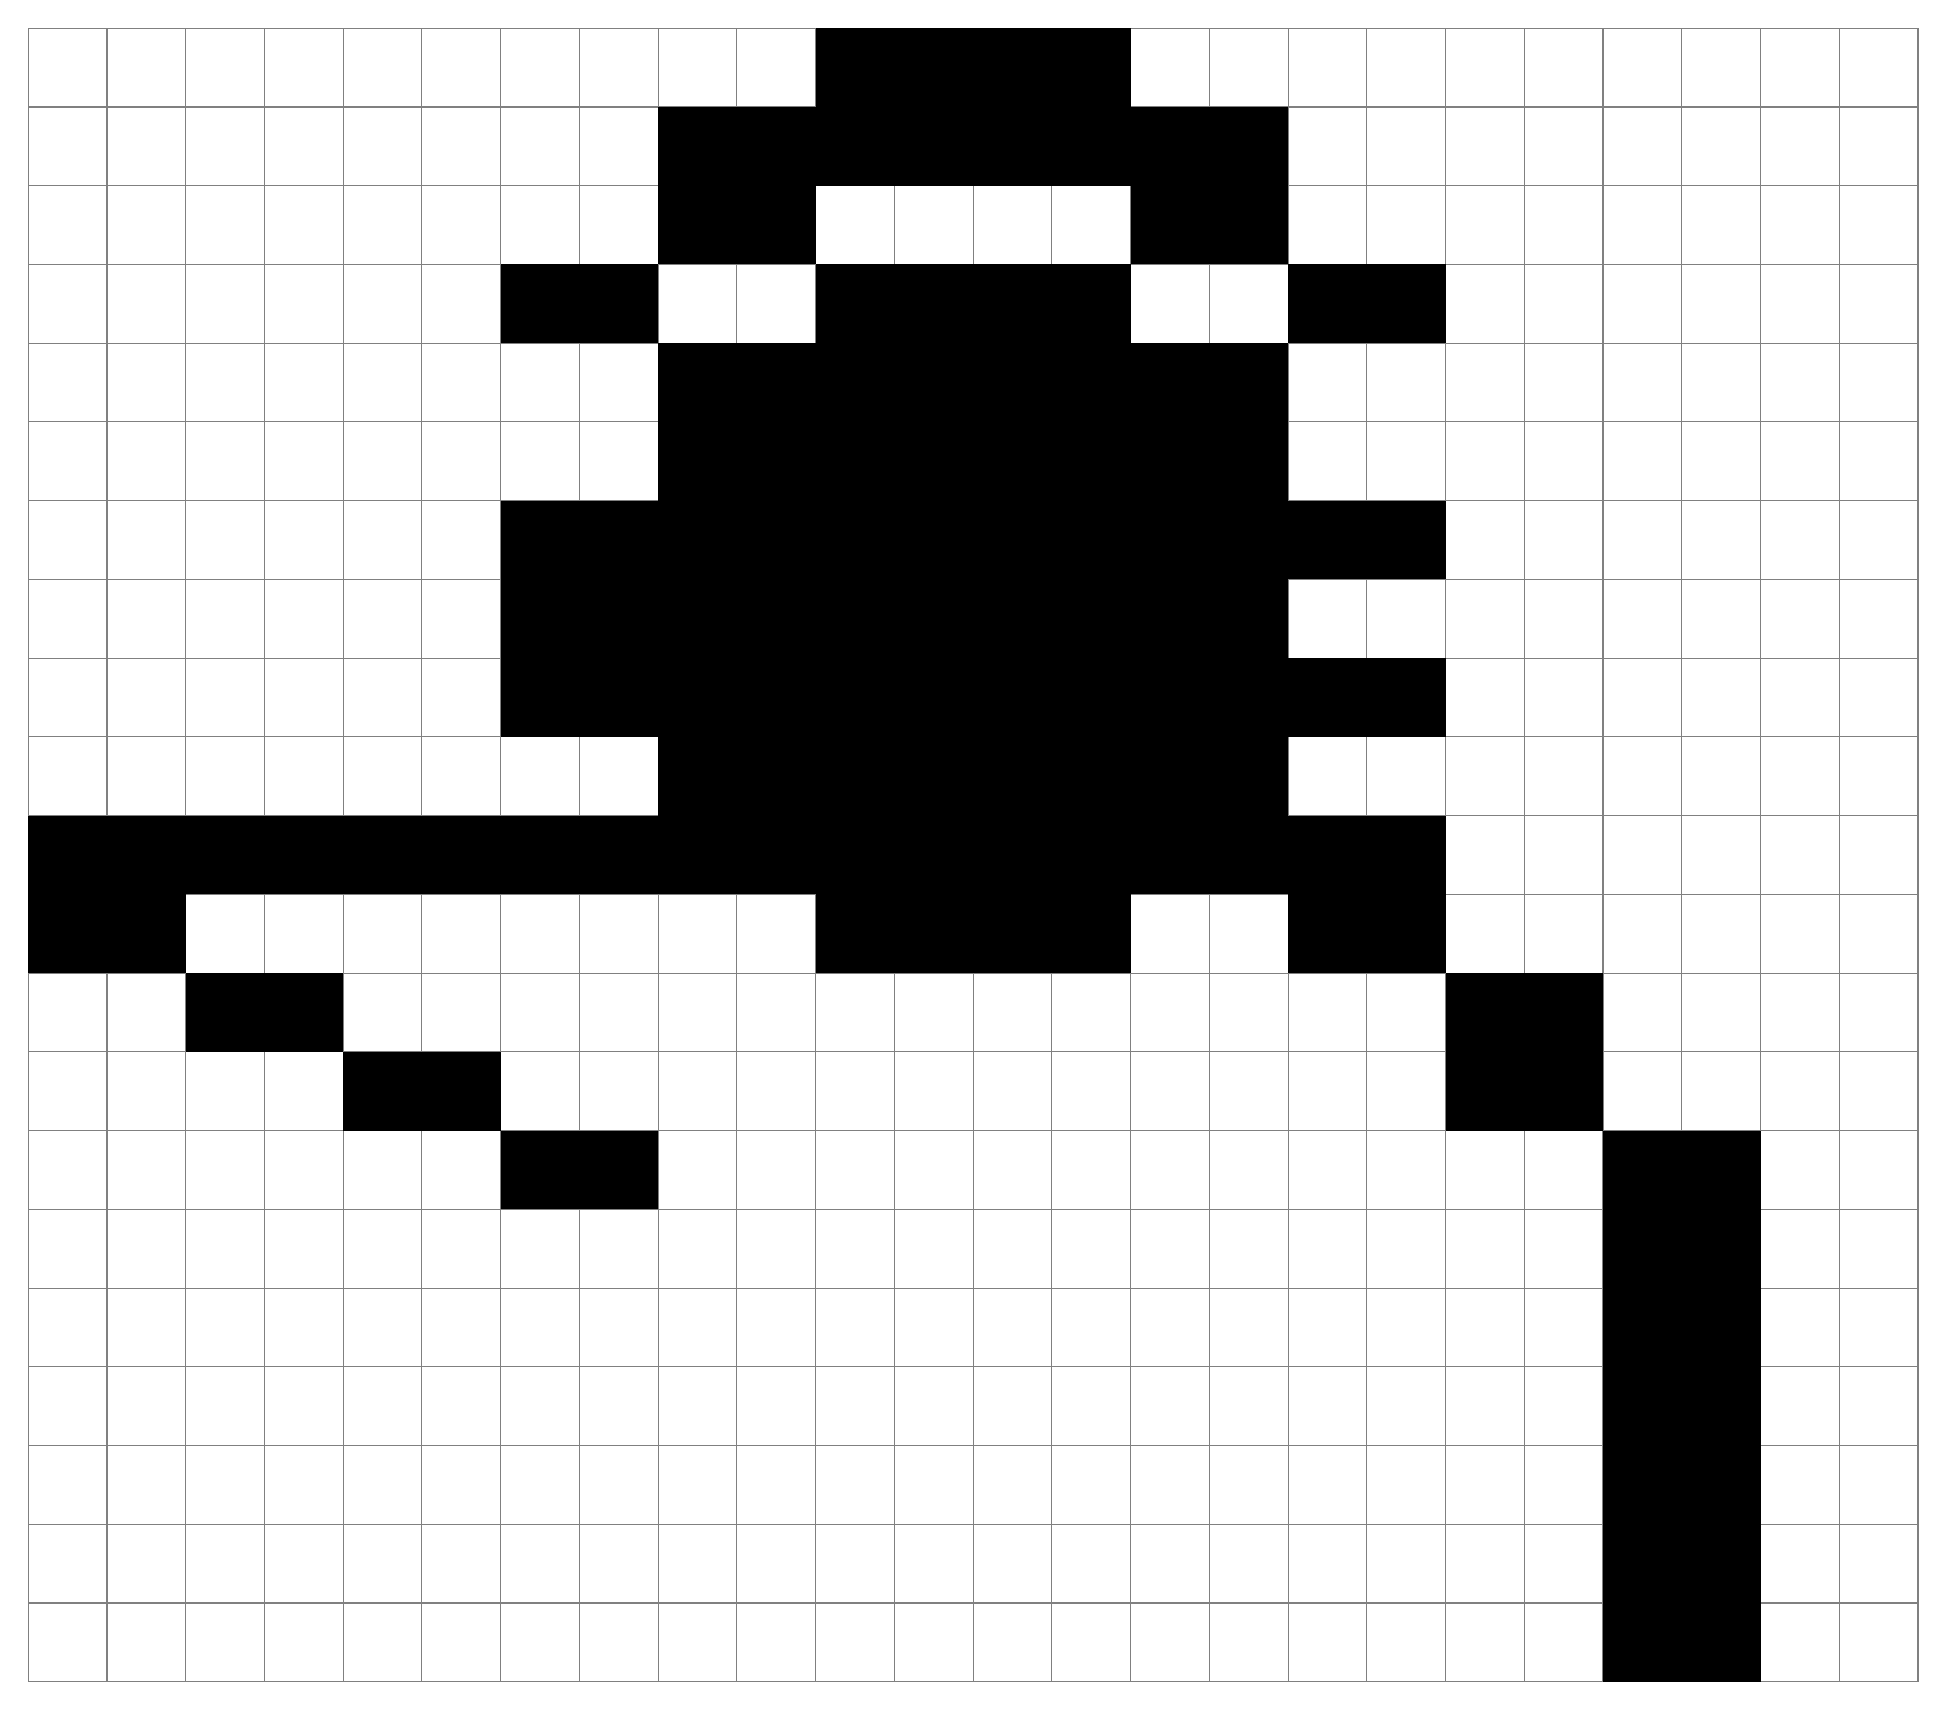
\begin{tikzpicture}

	\draw[step=1.0,gray,thin] (0,0) grid (24,21);
	\fill[\SPRITECOLOR] (10,20) rectangle ++ (1,1);
	\fill[\SPRITECOLOR] (11,20) rectangle ++ (1,1);
	\fill[\SPRITECOLOR] (12,20) rectangle ++ (1,1);
	\fill[\SPRITECOLOR] (13,20) rectangle ++ (1,1);
	\fill[\SPRITECOLOR] (8,19) rectangle ++ (1,1);
	\fill[\SPRITECOLOR] (9,19) rectangle ++ (1,1);
	\fill[\SPRITECOLOR] (10,19) rectangle ++ (1,1);
	\fill[\SPRITECOLOR] (11,19) rectangle ++ (1,1);
	\fill[\SPRITECOLOR] (12,19) rectangle ++ (1,1);
	\fill[\SPRITECOLOR] (13,19) rectangle ++ (1,1);
	\fill[\SPRITECOLOR] (14,19) rectangle ++ (1,1);
	\fill[\SPRITECOLOR] (15,19) rectangle ++ (1,1);
	\fill[\SPRITECOLOR] (8,18) rectangle ++ (1,1);
	\fill[\SPRITECOLOR] (9,18) rectangle ++ (1,1);
	\fill[\SPRITECOLOR] (14,18) rectangle ++ (1,1);
	\fill[\SPRITECOLOR] (15,18) rectangle ++ (1,1);
	\fill[\SPRITECOLOR] (6,17) rectangle ++ (1,1);
	\fill[\SPRITECOLOR] (7,17) rectangle ++ (1,1);
	\fill[\SPRITECOLOR] (10,17) rectangle ++ (1,1);
	\fill[\SPRITECOLOR] (11,17) rectangle ++ (1,1);
	\fill[\SPRITECOLOR] (12,17) rectangle ++ (1,1);
	\fill[\SPRITECOLOR] (13,17) rectangle ++ (1,1);
	\fill[\SPRITECOLOR] (16,17) rectangle ++ (1,1);
	\fill[\SPRITECOLOR] (17,17) rectangle ++ (1,1);
	\fill[\SPRITECOLOR] (8,16) rectangle ++ (1,1);
	\fill[\SPRITECOLOR] (9,16) rectangle ++ (1,1);
	\fill[\MULTICOLORTWO] (10,16) rectangle ++ (1,1);
	\fill[\MULTICOLORTWO] (11,16) rectangle ++ (1,1);
	\fill[\SPRITECOLOR] (12,16) rectangle ++ (1,1);
	\fill[\SPRITECOLOR] (13,16) rectangle ++ (1,1);
	\fill[\SPRITECOLOR] (14,16) rectangle ++ (1,1);
	\fill[\SPRITECOLOR] (15,16) rectangle ++ (1,1);
	\fill[\MULTICOLORTWO] (8,15) rectangle ++ (1,1);
	\fill[\MULTICOLORTWO] (9,15) rectangle ++ (1,1);
	\fill[\SPRITECOLOR] (10,15) rectangle ++ (1,1);
	\fill[\SPRITECOLOR] (11,15) rectangle ++ (1,1);
	\fill[\SPRITECOLOR] (12,15) rectangle ++ (1,1);
	\fill[\SPRITECOLOR] (13,15) rectangle ++ (1,1);
	\fill[\SPRITECOLOR] (14,15) rectangle ++ (1,1);
	\fill[\SPRITECOLOR] (15,15) rectangle ++ (1,1);
	\fill[\SPRITECOLOR] (6,14) rectangle ++ (1,1);
	\fill[\SPRITECOLOR] (7,14) rectangle ++ (1,1);
	\fill[\SPRITECOLOR] (8,14) rectangle ++ (1,1);
	\fill[\SPRITECOLOR] (9,14) rectangle ++ (1,1);
	\fill[\SPRITECOLOR] (10,14) rectangle ++ (1,1);
	\fill[\SPRITECOLOR] (11,14) rectangle ++ (1,1);
	\fill[\SPRITECOLOR] (12,14) rectangle ++ (1,1);
	\fill[\SPRITECOLOR] (13,14) rectangle ++ (1,1);
	\fill[\MULTICOLORTWO] (14,14) rectangle ++ (1,1);
	\fill[\MULTICOLORTWO] (15,14) rectangle ++ (1,1);
	\fill[\MULTICOLORTWO] (16,14) rectangle ++ (1,1);
	\fill[\MULTICOLORTWO] (17,14) rectangle ++ (1,1);
	\fill[\SPRITECOLOR] (6,13) rectangle ++ (1,1);
	\fill[\SPRITECOLOR] (7,13) rectangle ++ (1,1);
	\fill[\SPRITECOLOR] (8,13) rectangle ++ (1,1);
	\fill[\SPRITECOLOR] (9,13) rectangle ++ (1,1);
	\fill[\SPRITECOLOR] (10,13) rectangle ++ (1,1);
	\fill[\SPRITECOLOR] (11,13) rectangle ++ (1,1);
	\fill[\SPRITECOLOR] (12,13) rectangle ++ (1,1);
	\fill[\SPRITECOLOR] (13,13) rectangle ++ (1,1);
	\fill[\MULTICOLORTWO] (14,13) rectangle ++ (1,1);
	\fill[\MULTICOLORTWO] (15,13) rectangle ++ (1,1);
	\fill[\SPRITECOLOR] (6,12) rectangle ++ (1,1);
	\fill[\SPRITECOLOR] (7,12) rectangle ++ (1,1);
	\fill[\SPRITECOLOR] (8,12) rectangle ++ (1,1);
	\fill[\SPRITECOLOR] (9,12) rectangle ++ (1,1);
	\fill[\SPRITECOLOR] (10,12) rectangle ++ (1,1);
	\fill[\SPRITECOLOR] (11,12) rectangle ++ (1,1);
	\fill[\SPRITECOLOR] (12,12) rectangle ++ (1,1);
	\fill[\SPRITECOLOR] (13,12) rectangle ++ (1,1);
	\fill[\MULTICOLORTWO] (14,12) rectangle ++ (1,1);
	\fill[\MULTICOLORTWO] (15,12) rectangle ++ (1,1);
	\fill[\MULTICOLORTWO] (16,12) rectangle ++ (1,1);
	\fill[\MULTICOLORTWO] (17,12) rectangle ++ (1,1);
	\fill[\SPRITECOLOR] (8,11) rectangle ++ (1,1);
	\fill[\SPRITECOLOR] (9,11) rectangle ++ (1,1);
	\fill[\SPRITECOLOR] (10,11) rectangle ++ (1,1);
	\fill[\SPRITECOLOR] (11,11) rectangle ++ (1,1);
	\fill[\SPRITECOLOR] (12,11) rectangle ++ (1,1);
	\fill[\SPRITECOLOR] (13,11) rectangle ++ (1,1);
	\fill[\SPRITECOLOR] (14,11) rectangle ++ (1,1);
	\fill[\SPRITECOLOR] (15,11) rectangle ++ (1,1);
	\fill[\MULTICOLORTWO] (0,10) rectangle ++ (1,1);
	\fill[\MULTICOLORTWO] (1,10) rectangle ++ (1,1);
	\fill[\MULTICOLORONE] (2,10) rectangle ++ (1,1);
	\fill[\MULTICOLORONE] (3,10) rectangle ++ (1,1);
	\fill[\MULTICOLORONE] (4,10) rectangle ++ (1,1);
	\fill[\MULTICOLORONE] (5,10) rectangle ++ (1,1);
	\fill[\MULTICOLORONE] (6,10) rectangle ++ (1,1);
	\fill[\MULTICOLORONE] (7,10) rectangle ++ (1,1);
	\fill[\SPRITECOLOR] (8,10) rectangle ++ (1,1);
	\fill[\SPRITECOLOR] (9,10) rectangle ++ (1,1);
	\fill[\SPRITECOLOR] (10,10) rectangle ++ (1,1);
	\fill[\SPRITECOLOR] (11,10) rectangle ++ (1,1);
	\fill[\SPRITECOLOR] (12,10) rectangle ++ (1,1);
	\fill[\SPRITECOLOR] (13,10) rectangle ++ (1,1);
	\fill[\SPRITECOLOR] (14,10) rectangle ++ (1,1);
	\fill[\SPRITECOLOR] (15,10) rectangle ++ (1,1);
	\fill[\MULTICOLORONE] (16,10) rectangle ++ (1,1);
	\fill[\MULTICOLORONE] (17,10) rectangle ++ (1,1);
	\fill[\MULTICOLORONE] (0,9) rectangle ++ (1,1);
	\fill[\MULTICOLORONE] (1,9) rectangle ++ (1,1);
	\fill[\SPRITECOLOR] (10,9) rectangle ++ (1,1);
	\fill[\SPRITECOLOR] (11,9) rectangle ++ (1,1);
	\fill[\SPRITECOLOR] (12,9) rectangle ++ (1,1);
	\fill[\SPRITECOLOR] (13,9) rectangle ++ (1,1);
	\fill[\MULTICOLORONE] (16,9) rectangle ++ (1,1);
	\fill[\MULTICOLORONE] (17,9) rectangle ++ (1,1);
	\fill[\MULTICOLORONE] (2,8) rectangle ++ (1,1);
	\fill[\MULTICOLORONE] (3,8) rectangle ++ (1,1);
	\fill[\MULTICOLORONE] (18,8) rectangle ++ (1,1);
	\fill[\MULTICOLORONE] (19,8) rectangle ++ (1,1);
	\fill[\MULTICOLORONE] (4,7) rectangle ++ (1,1);
	\fill[\MULTICOLORONE] (5,7) rectangle ++ (1,1);
	\fill[\MULTICOLORONE] (18,7) rectangle ++ (1,1);
	\fill[\MULTICOLORONE] (19,7) rectangle ++ (1,1);
	\fill[\MULTICOLORONE] (6,6) rectangle ++ (1,1);
	\fill[\MULTICOLORONE] (7,6) rectangle ++ (1,1);
	\fill[\MULTICOLORTWO] (20,6) rectangle ++ (1,1);
	\fill[\MULTICOLORTWO] (21,6) rectangle ++ (1,1);
	\fill[\MULTICOLORONE] (20,5) rectangle ++ (1,1);
	\fill[\MULTICOLORONE] (21,5) rectangle ++ (1,1);
	\fill[\MULTICOLORONE] (20,4) rectangle ++ (1,1);
	\fill[\MULTICOLORONE] (21,4) rectangle ++ (1,1);
	\fill[\MULTICOLORONE] (20,3) rectangle ++ (1,1);
	\fill[\MULTICOLORONE] (21,3) rectangle ++ (1,1);
	\fill[\MULTICOLORONE] (20,2) rectangle ++ (1,1);
	\fill[\MULTICOLORONE] (21,2) rectangle ++ (1,1);
	\fill[\MULTICOLORONE] (20,1) rectangle ++ (1,1);
	\fill[\MULTICOLORONE] (21,1) rectangle ++ (1,1);
	\fill[\MULTICOLORONE] (20,0) rectangle ++ (1,1);
	\fill[\MULTICOLORONE] (21,0) rectangle ++ (1,1);

      \end{tikzpicture}
    \end{adjustbox}
  }\caption{LAND\_GILBY6}
\end{figure}

	\end{subfigure}
} & 
\makecell[l]{
	\begin{subfigure}{0.3\textwidth}
    \def\MULTICOLORONE{gray}
    \def\MULTICOLORTWO{white}
    \def\SPRITECOLOR{purple}
		
\begin{figure}[H]
  {
    \setlength{\tabcolsep}{3.0pt}
    \setlength\cmidrulewidth{\heavyrulewidth} % Make cmidrule = 
    \begin{adjustbox}{width=3cm,center}
      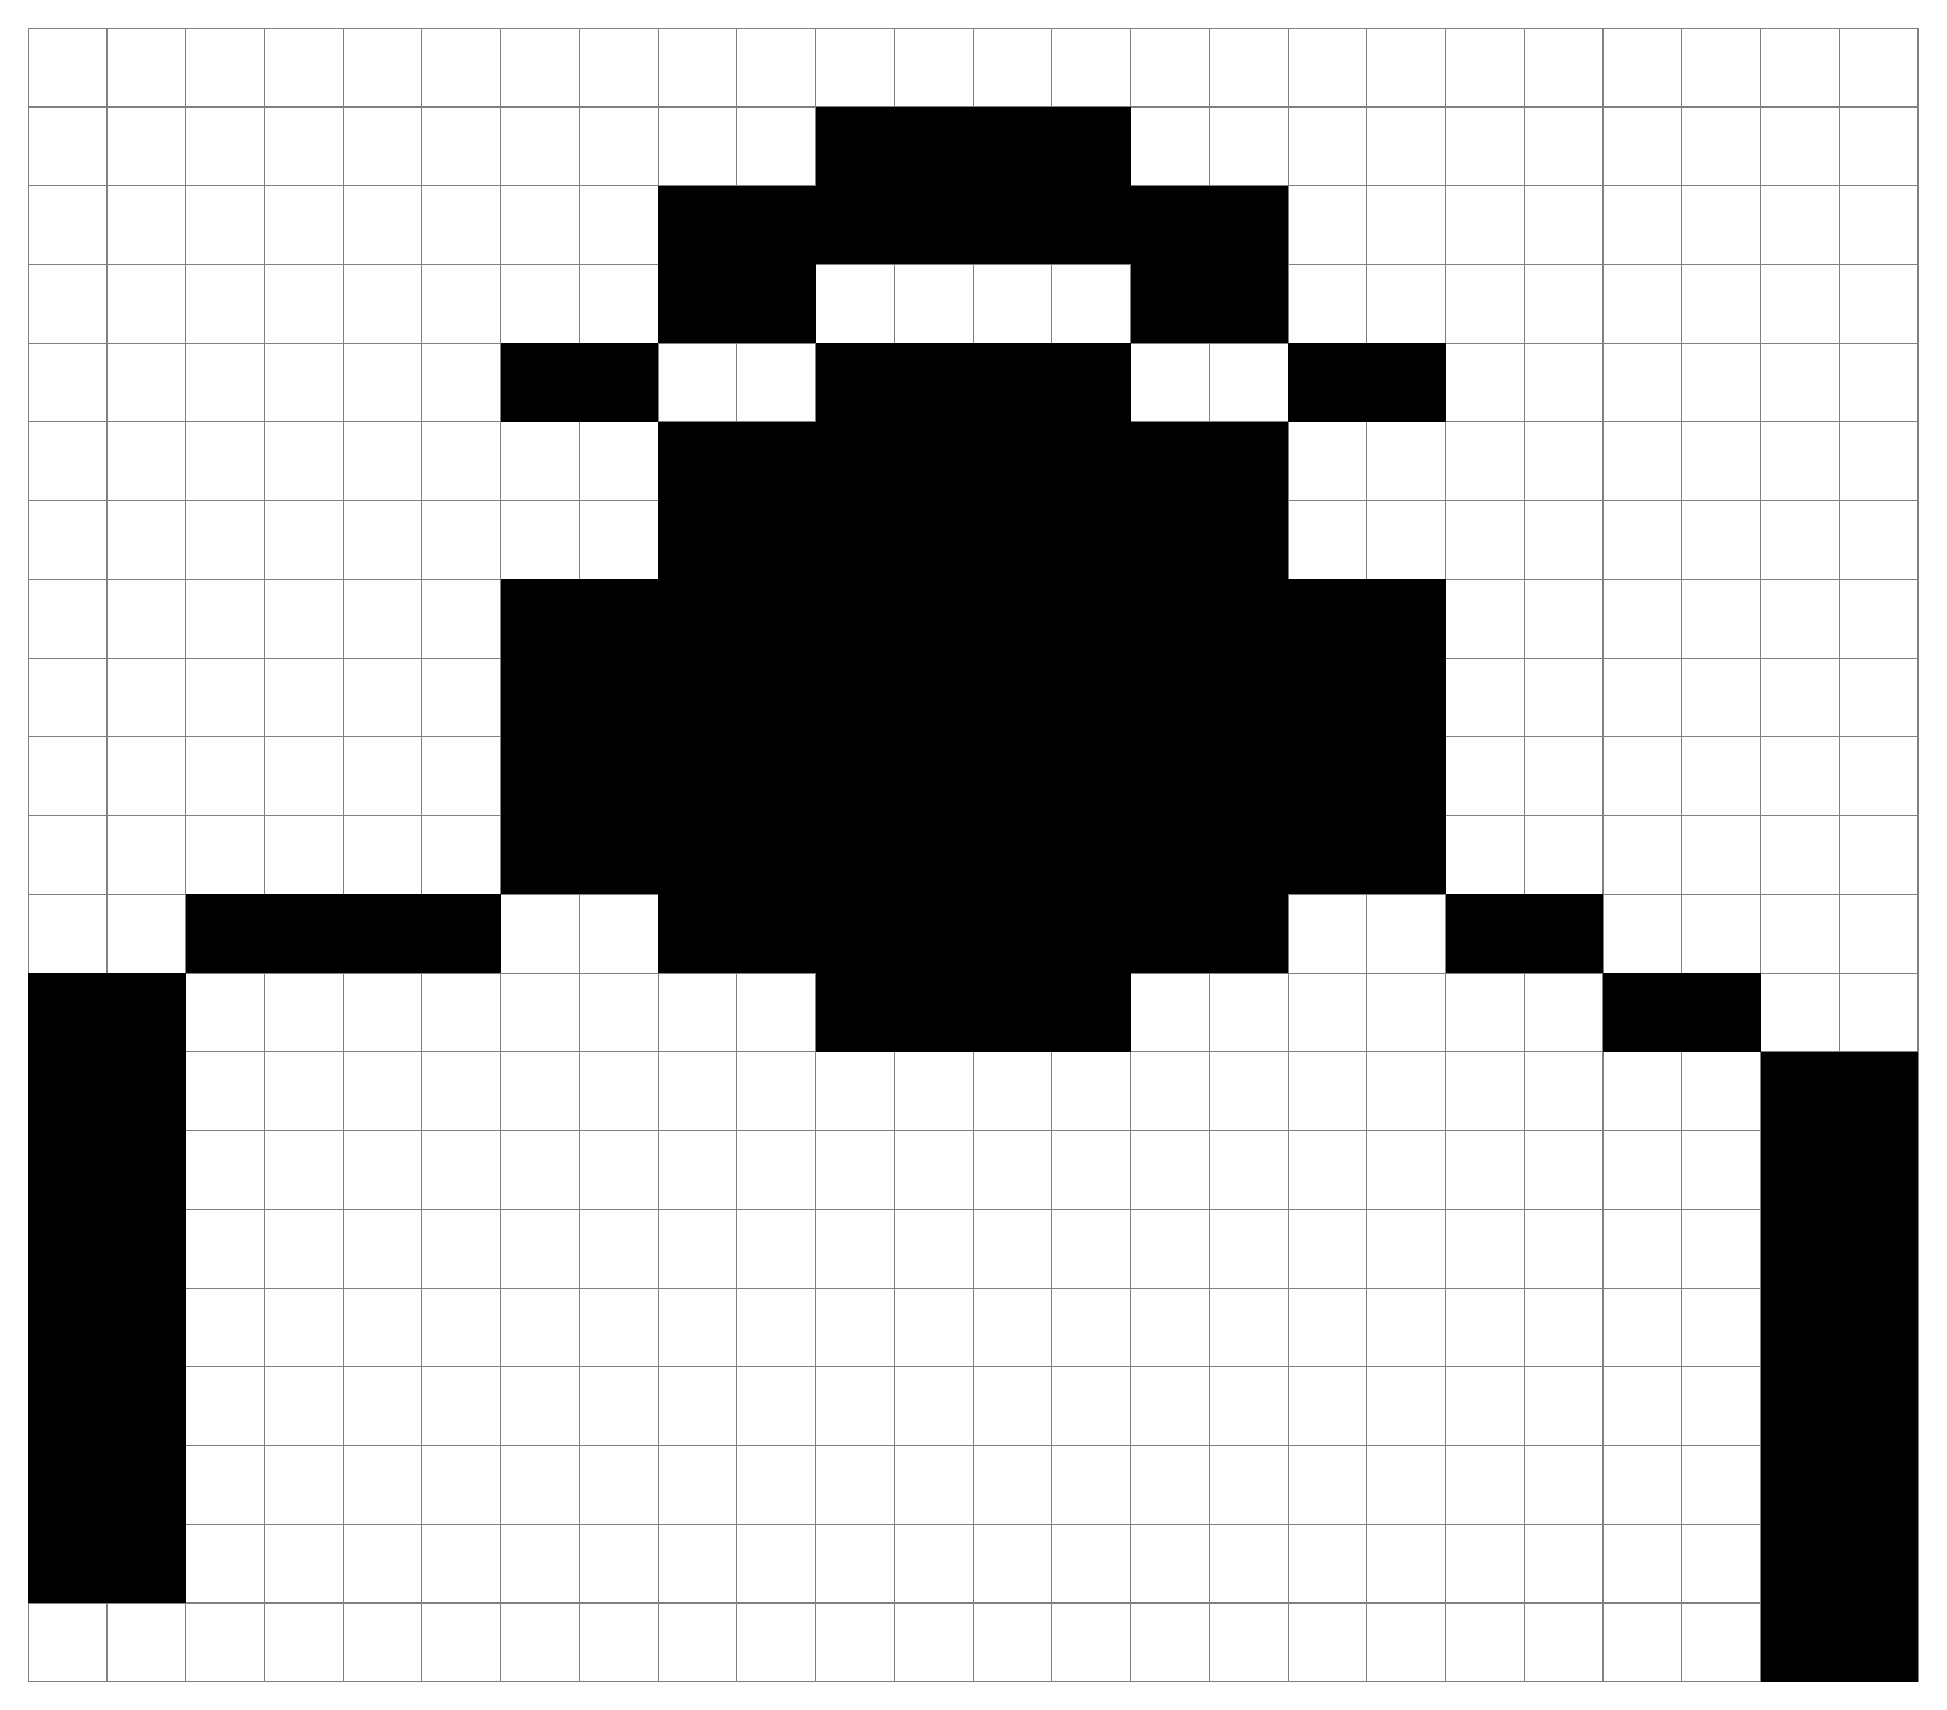
\begin{tikzpicture}

	\draw[step=1.0,gray,thin] (0,0) grid (24,21);
	\fill[\SPRITECOLOR] (10,19) rectangle ++ (1,1);
	\fill[\SPRITECOLOR] (11,19) rectangle ++ (1,1);
	\fill[\SPRITECOLOR] (12,19) rectangle ++ (1,1);
	\fill[\SPRITECOLOR] (13,19) rectangle ++ (1,1);
	\fill[\SPRITECOLOR] (8,18) rectangle ++ (1,1);
	\fill[\SPRITECOLOR] (9,18) rectangle ++ (1,1);
	\fill[\SPRITECOLOR] (10,18) rectangle ++ (1,1);
	\fill[\SPRITECOLOR] (11,18) rectangle ++ (1,1);
	\fill[\SPRITECOLOR] (12,18) rectangle ++ (1,1);
	\fill[\SPRITECOLOR] (13,18) rectangle ++ (1,1);
	\fill[\SPRITECOLOR] (14,18) rectangle ++ (1,1);
	\fill[\SPRITECOLOR] (15,18) rectangle ++ (1,1);
	\fill[\SPRITECOLOR] (8,17) rectangle ++ (1,1);
	\fill[\SPRITECOLOR] (9,17) rectangle ++ (1,1);
	\fill[\SPRITECOLOR] (14,17) rectangle ++ (1,1);
	\fill[\SPRITECOLOR] (15,17) rectangle ++ (1,1);
	\fill[\SPRITECOLOR] (6,16) rectangle ++ (1,1);
	\fill[\SPRITECOLOR] (7,16) rectangle ++ (1,1);
	\fill[\SPRITECOLOR] (10,16) rectangle ++ (1,1);
	\fill[\SPRITECOLOR] (11,16) rectangle ++ (1,1);
	\fill[\SPRITECOLOR] (12,16) rectangle ++ (1,1);
	\fill[\SPRITECOLOR] (13,16) rectangle ++ (1,1);
	\fill[\SPRITECOLOR] (16,16) rectangle ++ (1,1);
	\fill[\SPRITECOLOR] (17,16) rectangle ++ (1,1);
	\fill[\SPRITECOLOR] (8,15) rectangle ++ (1,1);
	\fill[\SPRITECOLOR] (9,15) rectangle ++ (1,1);
	\fill[\MULTICOLORTWO] (10,15) rectangle ++ (1,1);
	\fill[\MULTICOLORTWO] (11,15) rectangle ++ (1,1);
	\fill[\SPRITECOLOR] (12,15) rectangle ++ (1,1);
	\fill[\SPRITECOLOR] (13,15) rectangle ++ (1,1);
	\fill[\SPRITECOLOR] (14,15) rectangle ++ (1,1);
	\fill[\SPRITECOLOR] (15,15) rectangle ++ (1,1);
	\fill[\MULTICOLORTWO] (8,14) rectangle ++ (1,1);
	\fill[\MULTICOLORTWO] (9,14) rectangle ++ (1,1);
	\fill[\SPRITECOLOR] (10,14) rectangle ++ (1,1);
	\fill[\SPRITECOLOR] (11,14) rectangle ++ (1,1);
	\fill[\SPRITECOLOR] (12,14) rectangle ++ (1,1);
	\fill[\SPRITECOLOR] (13,14) rectangle ++ (1,1);
	\fill[\SPRITECOLOR] (14,14) rectangle ++ (1,1);
	\fill[\SPRITECOLOR] (15,14) rectangle ++ (1,1);
	\fill[\SPRITECOLOR] (6,13) rectangle ++ (1,1);
	\fill[\SPRITECOLOR] (7,13) rectangle ++ (1,1);
	\fill[\SPRITECOLOR] (8,13) rectangle ++ (1,1);
	\fill[\SPRITECOLOR] (9,13) rectangle ++ (1,1);
	\fill[\SPRITECOLOR] (10,13) rectangle ++ (1,1);
	\fill[\SPRITECOLOR] (11,13) rectangle ++ (1,1);
	\fill[\SPRITECOLOR] (12,13) rectangle ++ (1,1);
	\fill[\SPRITECOLOR] (13,13) rectangle ++ (1,1);
	\fill[\SPRITECOLOR] (14,13) rectangle ++ (1,1);
	\fill[\SPRITECOLOR] (15,13) rectangle ++ (1,1);
	\fill[\SPRITECOLOR] (16,13) rectangle ++ (1,1);
	\fill[\SPRITECOLOR] (17,13) rectangle ++ (1,1);
	\fill[\SPRITECOLOR] (6,12) rectangle ++ (1,1);
	\fill[\SPRITECOLOR] (7,12) rectangle ++ (1,1);
	\fill[\SPRITECOLOR] (8,12) rectangle ++ (1,1);
	\fill[\SPRITECOLOR] (9,12) rectangle ++ (1,1);
	\fill[\SPRITECOLOR] (10,12) rectangle ++ (1,1);
	\fill[\SPRITECOLOR] (11,12) rectangle ++ (1,1);
	\fill[\SPRITECOLOR] (12,12) rectangle ++ (1,1);
	\fill[\SPRITECOLOR] (13,12) rectangle ++ (1,1);
	\fill[\SPRITECOLOR] (14,12) rectangle ++ (1,1);
	\fill[\SPRITECOLOR] (15,12) rectangle ++ (1,1);
	\fill[\SPRITECOLOR] (16,12) rectangle ++ (1,1);
	\fill[\SPRITECOLOR] (17,12) rectangle ++ (1,1);
	\fill[\SPRITECOLOR] (6,11) rectangle ++ (1,1);
	\fill[\SPRITECOLOR] (7,11) rectangle ++ (1,1);
	\fill[\SPRITECOLOR] (8,11) rectangle ++ (1,1);
	\fill[\SPRITECOLOR] (9,11) rectangle ++ (1,1);
	\fill[\SPRITECOLOR] (10,11) rectangle ++ (1,1);
	\fill[\SPRITECOLOR] (11,11) rectangle ++ (1,1);
	\fill[\SPRITECOLOR] (12,11) rectangle ++ (1,1);
	\fill[\SPRITECOLOR] (13,11) rectangle ++ (1,1);
	\fill[\SPRITECOLOR] (14,11) rectangle ++ (1,1);
	\fill[\SPRITECOLOR] (15,11) rectangle ++ (1,1);
	\fill[\SPRITECOLOR] (16,11) rectangle ++ (1,1);
	\fill[\SPRITECOLOR] (17,11) rectangle ++ (1,1);
	\fill[\MULTICOLORONE] (6,10) rectangle ++ (1,1);
	\fill[\MULTICOLORONE] (7,10) rectangle ++ (1,1);
	\fill[\SPRITECOLOR] (8,10) rectangle ++ (1,1);
	\fill[\SPRITECOLOR] (9,10) rectangle ++ (1,1);
	\fill[\SPRITECOLOR] (10,10) rectangle ++ (1,1);
	\fill[\SPRITECOLOR] (11,10) rectangle ++ (1,1);
	\fill[\SPRITECOLOR] (12,10) rectangle ++ (1,1);
	\fill[\SPRITECOLOR] (13,10) rectangle ++ (1,1);
	\fill[\SPRITECOLOR] (14,10) rectangle ++ (1,1);
	\fill[\SPRITECOLOR] (15,10) rectangle ++ (1,1);
	\fill[\MULTICOLORONE] (16,10) rectangle ++ (1,1);
	\fill[\MULTICOLORONE] (17,10) rectangle ++ (1,1);
	\fill[\MULTICOLORONE] (2,9) rectangle ++ (1,1);
	\fill[\MULTICOLORONE] (3,9) rectangle ++ (1,1);
	\fill[\MULTICOLORONE] (4,9) rectangle ++ (1,1);
	\fill[\MULTICOLORONE] (5,9) rectangle ++ (1,1);
	\fill[\SPRITECOLOR] (8,9) rectangle ++ (1,1);
	\fill[\SPRITECOLOR] (9,9) rectangle ++ (1,1);
	\fill[\SPRITECOLOR] (10,9) rectangle ++ (1,1);
	\fill[\SPRITECOLOR] (11,9) rectangle ++ (1,1);
	\fill[\SPRITECOLOR] (12,9) rectangle ++ (1,1);
	\fill[\SPRITECOLOR] (13,9) rectangle ++ (1,1);
	\fill[\SPRITECOLOR] (14,9) rectangle ++ (1,1);
	\fill[\SPRITECOLOR] (15,9) rectangle ++ (1,1);
	\fill[\MULTICOLORONE] (18,9) rectangle ++ (1,1);
	\fill[\MULTICOLORONE] (19,9) rectangle ++ (1,1);
	\fill[\MULTICOLORTWO] (0,8) rectangle ++ (1,1);
	\fill[\MULTICOLORTWO] (1,8) rectangle ++ (1,1);
	\fill[\SPRITECOLOR] (10,8) rectangle ++ (1,1);
	\fill[\SPRITECOLOR] (11,8) rectangle ++ (1,1);
	\fill[\SPRITECOLOR] (12,8) rectangle ++ (1,1);
	\fill[\SPRITECOLOR] (13,8) rectangle ++ (1,1);
	\fill[\MULTICOLORONE] (20,8) rectangle ++ (1,1);
	\fill[\MULTICOLORONE] (21,8) rectangle ++ (1,1);
	\fill[\MULTICOLORONE] (0,7) rectangle ++ (1,1);
	\fill[\MULTICOLORONE] (1,7) rectangle ++ (1,1);
	\fill[\MULTICOLORTWO] (22,7) rectangle ++ (1,1);
	\fill[\MULTICOLORTWO] (23,7) rectangle ++ (1,1);
	\fill[\MULTICOLORONE] (0,6) rectangle ++ (1,1);
	\fill[\MULTICOLORONE] (1,6) rectangle ++ (1,1);
	\fill[\MULTICOLORONE] (22,6) rectangle ++ (1,1);
	\fill[\MULTICOLORONE] (23,6) rectangle ++ (1,1);
	\fill[\MULTICOLORONE] (0,5) rectangle ++ (1,1);
	\fill[\MULTICOLORONE] (1,5) rectangle ++ (1,1);
	\fill[\MULTICOLORONE] (22,5) rectangle ++ (1,1);
	\fill[\MULTICOLORONE] (23,5) rectangle ++ (1,1);
	\fill[\MULTICOLORONE] (0,4) rectangle ++ (1,1);
	\fill[\MULTICOLORONE] (1,4) rectangle ++ (1,1);
	\fill[\MULTICOLORONE] (22,4) rectangle ++ (1,1);
	\fill[\MULTICOLORONE] (23,4) rectangle ++ (1,1);
	\fill[\MULTICOLORONE] (0,3) rectangle ++ (1,1);
	\fill[\MULTICOLORONE] (1,3) rectangle ++ (1,1);
	\fill[\MULTICOLORONE] (22,3) rectangle ++ (1,1);
	\fill[\MULTICOLORONE] (23,3) rectangle ++ (1,1);
	\fill[\MULTICOLORONE] (0,2) rectangle ++ (1,1);
	\fill[\MULTICOLORONE] (1,2) rectangle ++ (1,1);
	\fill[\MULTICOLORONE] (22,2) rectangle ++ (1,1);
	\fill[\MULTICOLORONE] (23,2) rectangle ++ (1,1);
	\fill[\MULTICOLORONE] (0,1) rectangle ++ (1,1);
	\fill[\MULTICOLORONE] (1,1) rectangle ++ (1,1);
	\fill[\MULTICOLORONE] (22,1) rectangle ++ (1,1);
	\fill[\MULTICOLORONE] (23,1) rectangle ++ (1,1);
	\fill[\MULTICOLORONE] (22,0) rectangle ++ (1,1);
	\fill[\MULTICOLORONE] (23,0) rectangle ++ (1,1);

      \end{tikzpicture}
    \end{adjustbox}
  }\caption{LAND\_GILBY7}
\end{figure}

	\end{subfigure}
} \\ 
        \addlinespace
        \bottomrule
      \end{tabular}
    \end{adjustbox}
  }\caption{The sprites used by the top half of the screen and the bottom half of the screen.}
\end{figure}

The eighth sprite (Sprite 7) is used on both halves of the screen to display the starfield. This
sprite pushes right up against the line limitation. It's painted at intervals throughout the screen
but we're careful to avoid it ever being painted twice on the same line. We'll see how this is
achieved very soon.


\begin{figure}[H]
  {
    \setlength{\tabcolsep}{1.0pt}
    \setlength\cmidrulewidth{\heavyrulewidth} % Make cmidrule = 
    \begin{adjustbox}{width=4cm,center}
	\begin{subfigure}{0.3\textwidth}
    \def\MULTICOLORONE{gray}
    \def\MULTICOLORTWO{gray}
    \def\SPRITECOLOR{gray}
		
\begin{figure}[H]
  {
    \setlength{\tabcolsep}{3.0pt}
    \setlength\cmidrulewidth{\heavyrulewidth} % Make cmidrule = 
    \begin{adjustbox}{width=3cm,center}
      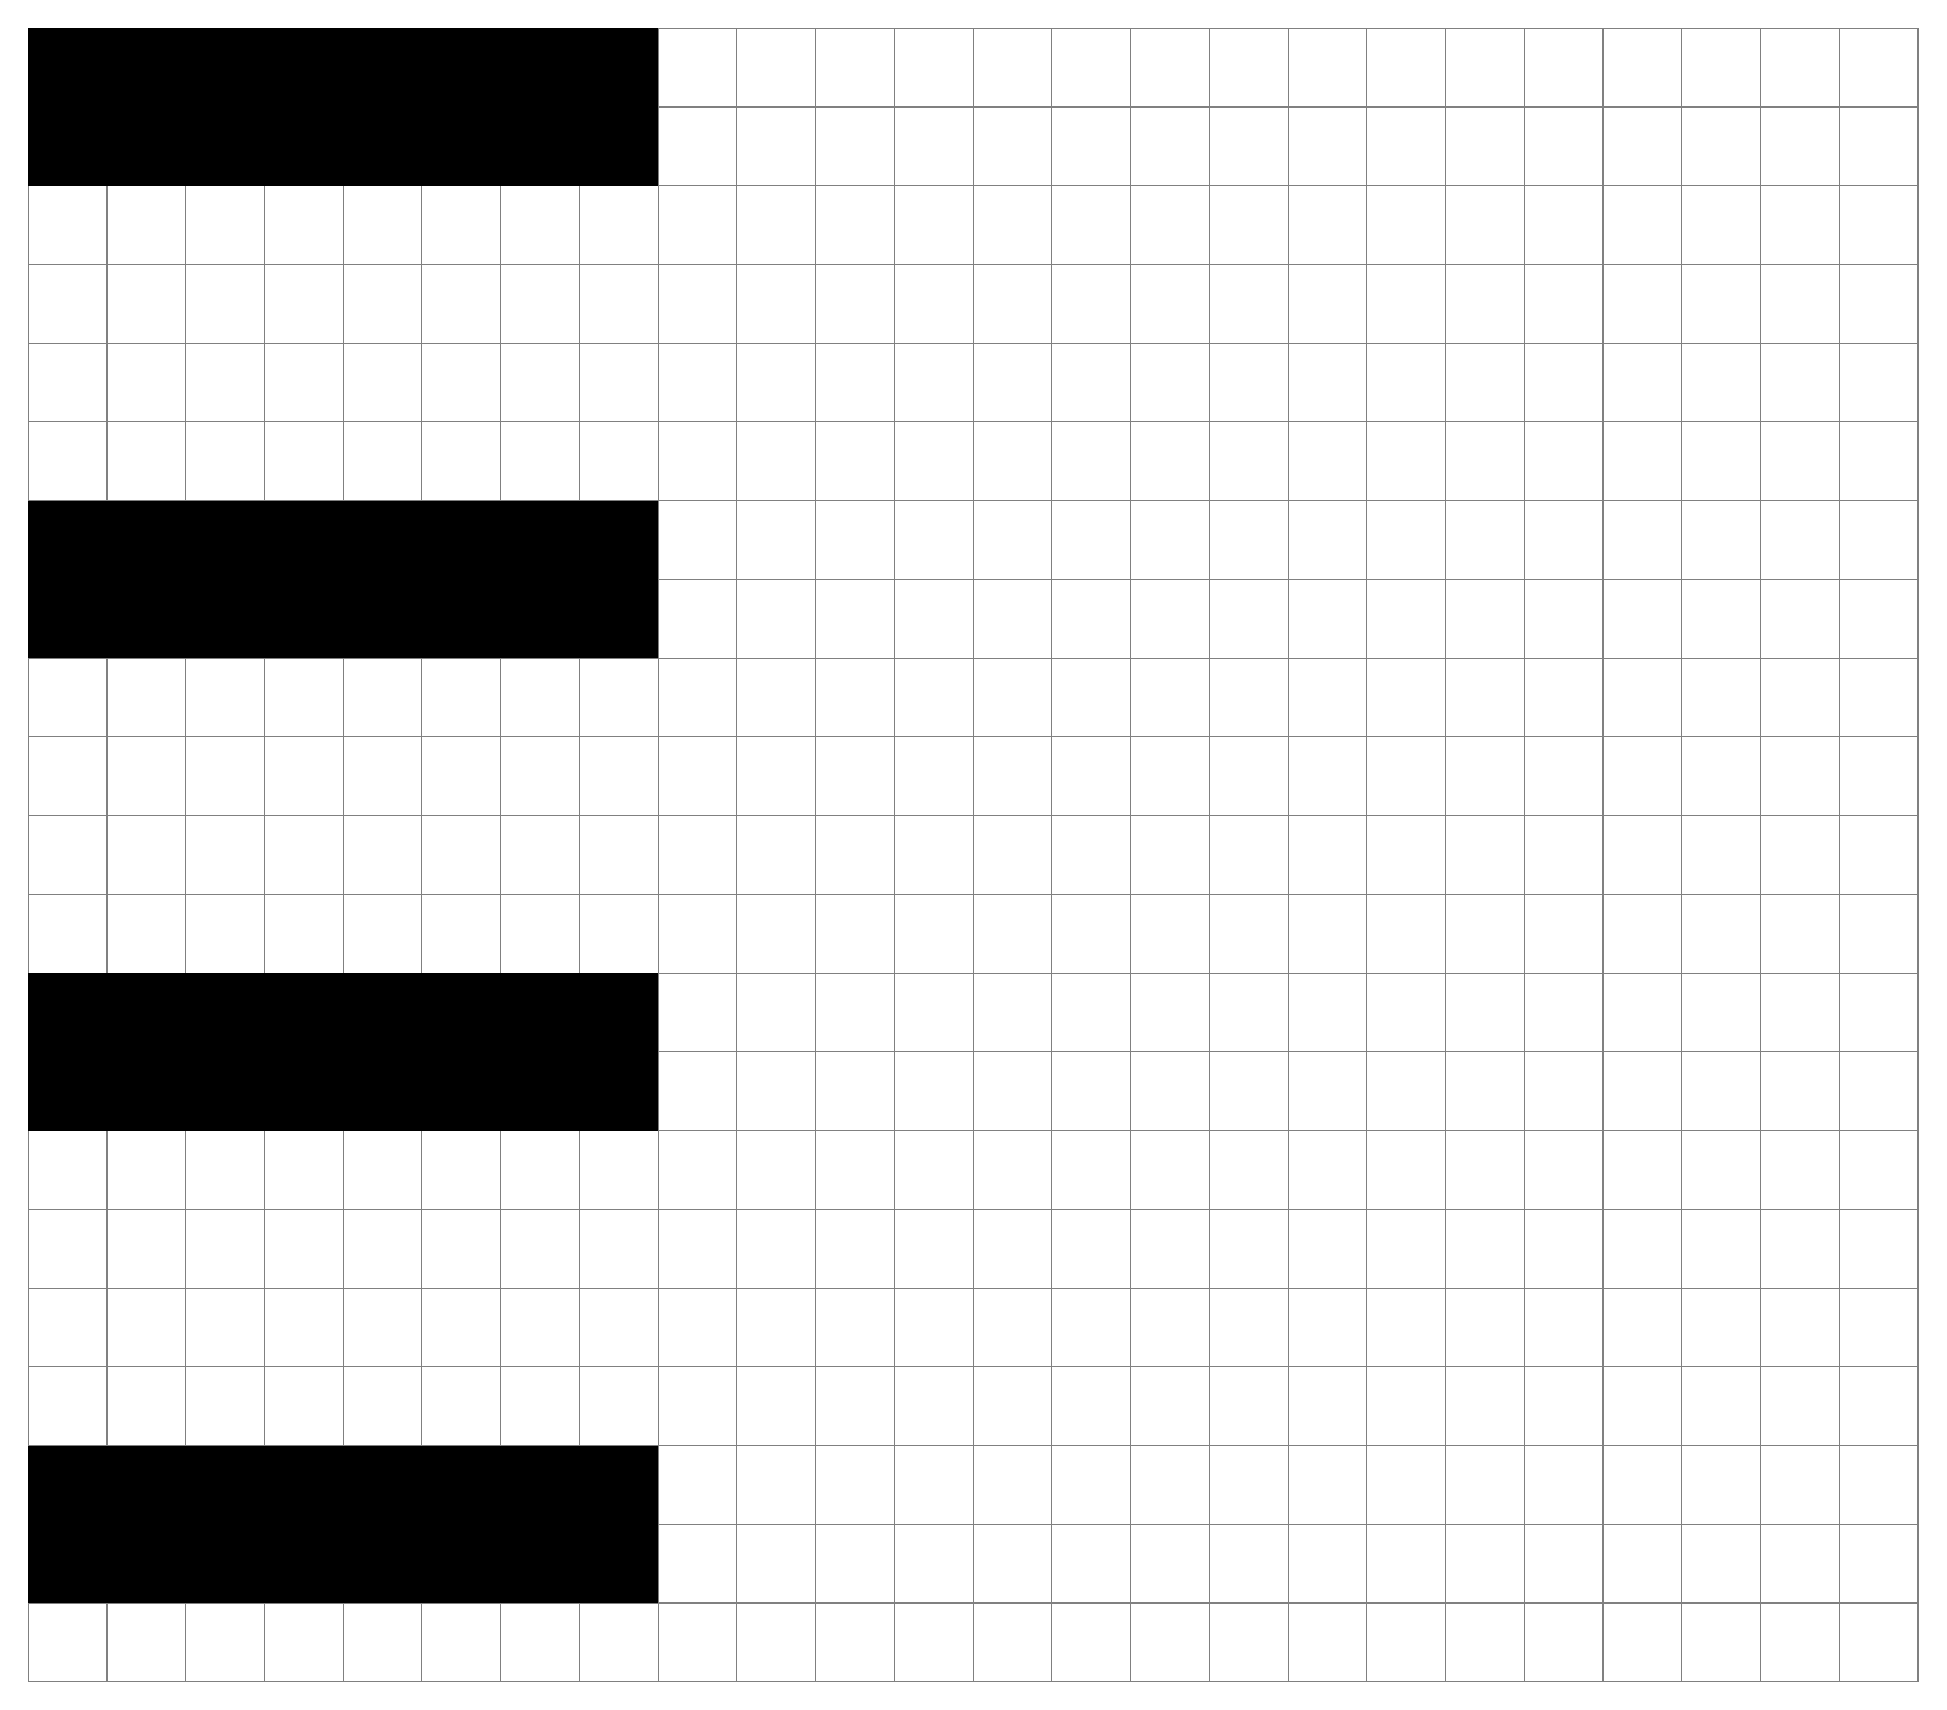
\begin{tikzpicture}

	\draw[step=1.0,gray,thin] (0,0) grid (24,21);
	\fill[\MULTICOLORTWO] (0,20) rectangle ++ (1,1);
	\fill[\MULTICOLORTWO] (1,20) rectangle ++ (1,1);
	\fill[\MULTICOLORTWO] (2,20) rectangle ++ (1,1);
	\fill[\MULTICOLORTWO] (3,20) rectangle ++ (1,1);
	\fill[\MULTICOLORTWO] (4,20) rectangle ++ (1,1);
	\fill[\MULTICOLORTWO] (5,20) rectangle ++ (1,1);
	\fill[\SPRITECOLOR] (6,20) rectangle ++ (1,1);
	\fill[\SPRITECOLOR] (7,20) rectangle ++ (1,1);
	\fill[\MULTICOLORTWO] (0,19) rectangle ++ (1,1);
	\fill[\MULTICOLORTWO] (1,19) rectangle ++ (1,1);
	\fill[\MULTICOLORTWO] (2,19) rectangle ++ (1,1);
	\fill[\MULTICOLORTWO] (3,19) rectangle ++ (1,1);
	\fill[\MULTICOLORTWO] (4,19) rectangle ++ (1,1);
	\fill[\MULTICOLORTWO] (5,19) rectangle ++ (1,1);
	\fill[\SPRITECOLOR] (6,19) rectangle ++ (1,1);
	\fill[\SPRITECOLOR] (7,19) rectangle ++ (1,1);
	\fill[\MULTICOLORTWO] (0,14) rectangle ++ (1,1);
	\fill[\MULTICOLORTWO] (1,14) rectangle ++ (1,1);
	\fill[\MULTICOLORTWO] (2,14) rectangle ++ (1,1);
	\fill[\MULTICOLORTWO] (3,14) rectangle ++ (1,1);
	\fill[\MULTICOLORTWO] (4,14) rectangle ++ (1,1);
	\fill[\MULTICOLORTWO] (5,14) rectangle ++ (1,1);
	\fill[\SPRITECOLOR] (6,14) rectangle ++ (1,1);
	\fill[\SPRITECOLOR] (7,14) rectangle ++ (1,1);
	\fill[\MULTICOLORTWO] (0,13) rectangle ++ (1,1);
	\fill[\MULTICOLORTWO] (1,13) rectangle ++ (1,1);
	\fill[\MULTICOLORTWO] (2,13) rectangle ++ (1,1);
	\fill[\MULTICOLORTWO] (3,13) rectangle ++ (1,1);
	\fill[\MULTICOLORTWO] (4,13) rectangle ++ (1,1);
	\fill[\MULTICOLORTWO] (5,13) rectangle ++ (1,1);
	\fill[\SPRITECOLOR] (6,13) rectangle ++ (1,1);
	\fill[\SPRITECOLOR] (7,13) rectangle ++ (1,1);
	\fill[\MULTICOLORTWO] (0,8) rectangle ++ (1,1);
	\fill[\MULTICOLORTWO] (1,8) rectangle ++ (1,1);
	\fill[\MULTICOLORTWO] (2,8) rectangle ++ (1,1);
	\fill[\MULTICOLORTWO] (3,8) rectangle ++ (1,1);
	\fill[\MULTICOLORTWO] (4,8) rectangle ++ (1,1);
	\fill[\MULTICOLORTWO] (5,8) rectangle ++ (1,1);
	\fill[\SPRITECOLOR] (6,8) rectangle ++ (1,1);
	\fill[\SPRITECOLOR] (7,8) rectangle ++ (1,1);
	\fill[\MULTICOLORTWO] (0,7) rectangle ++ (1,1);
	\fill[\MULTICOLORTWO] (1,7) rectangle ++ (1,1);
	\fill[\MULTICOLORTWO] (2,7) rectangle ++ (1,1);
	\fill[\MULTICOLORTWO] (3,7) rectangle ++ (1,1);
	\fill[\MULTICOLORTWO] (4,7) rectangle ++ (1,1);
	\fill[\MULTICOLORTWO] (5,7) rectangle ++ (1,1);
	\fill[\SPRITECOLOR] (6,7) rectangle ++ (1,1);
	\fill[\SPRITECOLOR] (7,7) rectangle ++ (1,1);
	\fill[\MULTICOLORTWO] (0,2) rectangle ++ (1,1);
	\fill[\MULTICOLORTWO] (1,2) rectangle ++ (1,1);
	\fill[\MULTICOLORTWO] (2,2) rectangle ++ (1,1);
	\fill[\MULTICOLORTWO] (3,2) rectangle ++ (1,1);
	\fill[\MULTICOLORTWO] (4,2) rectangle ++ (1,1);
	\fill[\MULTICOLORTWO] (5,2) rectangle ++ (1,1);
	\fill[\SPRITECOLOR] (6,2) rectangle ++ (1,1);
	\fill[\SPRITECOLOR] (7,2) rectangle ++ (1,1);
	\fill[\MULTICOLORTWO] (0,1) rectangle ++ (1,1);
	\fill[\MULTICOLORTWO] (1,1) rectangle ++ (1,1);
	\fill[\MULTICOLORTWO] (2,1) rectangle ++ (1,1);
	\fill[\MULTICOLORTWO] (3,1) rectangle ++ (1,1);
	\fill[\MULTICOLORTWO] (4,1) rectangle ++ (1,1);
	\fill[\MULTICOLORTWO] (5,1) rectangle ++ (1,1);
	\fill[\SPRITECOLOR] (6,1) rectangle ++ (1,1);
	\fill[\SPRITECOLOR] (7,1) rectangle ++ (1,1);

      \end{tikzpicture}
    \end{adjustbox}
  }\caption{STARFIELD\_SPRITE}
\end{figure}

	\end{subfigure}
    \end{adjustbox}
  }\caption{The sprite used for painting the starfield. Only a part of the sprite is ever painted!}
\end{figure}

\subsection{Waiting for the Beam}
With our 'Raster Interrupt' handler set up as \icode{TitleScreenInterruptHandler} we're ready to 
react when the raster reaches line 16 on the screen. Since the screen is made up of 512 lines in
total this will be along soon.

Before it comes in we just have time to prepare the relatively light amount of text we want displayed
on the screen in memory. We only need to do this once. Throughout the code we refer to this
area we write to as \icode{SCREEN\_RAM}. It's an address range between \icode{\$0400} and \icode{\$07E8} This is a very
simple bitmap representation of the entire screen that is 40 characters wide and 25 characters wide,
giving a total of 1000 bytes (\$3E8 bytes in hex). If we wanted to think of it as pixels it is 320 pixels wide (40 * 8)
and 200 pixels high (25 * 8). The important thing to remember about this \icode{SCREEN\_RAM} is that it is solely
for storing what we call character data. You can think of character data as 'text'. This text gets painted
first and then sprites get painted on top of it.

In \icode{EnterTitleScreenLoop} we call two routines that will prepare the character data for the raster to paint. 

The first, \icode{DrawStripesBehindTitle} writes the rainbow stripes to five lines in the top half of the screen. 
The second, \icode{DrawTitleScreenText} writes some text to the bottom half of the screen. Before we look at these
in detail we need to understand how this thing \icode{SCREEN\_RAM} works and how we store characters for display in it.

Our starting point for displaying text on screen is to define what our characters look like. We define the appearance
of a character using 8 bytes. This is what the definition of the stripe character looks like: 

\begin{lstlisting}[caption= The 'stripe' character.,basicstyle=\tiny]
characterSetData
        .BYTE $FF,$00,$FF,$00,$00,$FF,$00,$FF   ;.BYTE $FF,$00,$FF,$00,$00,$FF,$00,$FF
                                                ; CHARACTER $00
                                                ; 11111111   ********
                                                ; 00000000           
                                                ; 11111111   ********
                                                ; 00000000           
                                                ; 00000000           
                                                ; 11111111   ********
                                                ; 00000000           
                                                ; 11111111   ********
\end{lstlisting}

As you can see each byte translates to a row of 0s and 1s. Each 1 defines a dot and each 0 a blank space. We end up
with a character that is 8 pixels wide and 8 pixels high:


    \begin{figure}[H]
      {
        \setlength{\tabcolsep}{3.0pt}
        \setlength\cmidrulewidth{\lightrulewidth} % Make cmidrule = 
        \begin{adjustbox}{width=6cm,center}
          \begin{tikzpicture}
    
\def\CHARCOLOR{lightgray}
	\draw[step=1.0,gray,thin] (0,0) grid (8,8);
	\fill[\CHARCOLOR] (0,7) rectangle ++ (1,1);
	\fill[\CHARCOLOR] (1,7) rectangle ++ (1,1);
	\fill[\CHARCOLOR] (2,7) rectangle ++ (1,1);
	\fill[\CHARCOLOR] (3,7) rectangle ++ (1,1);
	\fill[\CHARCOLOR] (4,7) rectangle ++ (1,1);
	\fill[\CHARCOLOR] (5,7) rectangle ++ (1,1);
	\fill[\CHARCOLOR] (6,7) rectangle ++ (1,1);
	\fill[\CHARCOLOR] (7,7) rectangle ++ (1,1);
	\fill[\CHARCOLOR] (0,5) rectangle ++ (1,1);
	\fill[\CHARCOLOR] (1,5) rectangle ++ (1,1);
	\fill[\CHARCOLOR] (2,5) rectangle ++ (1,1);
	\fill[\CHARCOLOR] (3,5) rectangle ++ (1,1);
	\fill[\CHARCOLOR] (4,5) rectangle ++ (1,1);
	\fill[\CHARCOLOR] (5,5) rectangle ++ (1,1);
	\fill[\CHARCOLOR] (6,5) rectangle ++ (1,1);
	\fill[\CHARCOLOR] (7,5) rectangle ++ (1,1);
	\fill[\CHARCOLOR] (0,2) rectangle ++ (1,1);
	\fill[\CHARCOLOR] (1,2) rectangle ++ (1,1);
	\fill[\CHARCOLOR] (2,2) rectangle ++ (1,1);
	\fill[\CHARCOLOR] (3,2) rectangle ++ (1,1);
	\fill[\CHARCOLOR] (4,2) rectangle ++ (1,1);
	\fill[\CHARCOLOR] (5,2) rectangle ++ (1,1);
	\fill[\CHARCOLOR] (6,2) rectangle ++ (1,1);
	\fill[\CHARCOLOR] (7,2) rectangle ++ (1,1);
	\fill[\CHARCOLOR] (0,0) rectangle ++ (1,1);
	\fill[\CHARCOLOR] (1,0) rectangle ++ (1,1);
	\fill[\CHARCOLOR] (2,0) rectangle ++ (1,1);
	\fill[\CHARCOLOR] (3,0) rectangle ++ (1,1);
	\fill[\CHARCOLOR] (4,0) rectangle ++ (1,1);
	\fill[\CHARCOLOR] (5,0) rectangle ++ (1,1);
	\fill[\CHARCOLOR] (6,0) rectangle ++ (1,1);
	\fill[\CHARCOLOR] (7,0) rectangle ++ (1,1);
        \node[matrix of math nodes,anchor=south west,inner sep=0pt,
        nodes={draw,minimum size=1cm,anchor=center},
        column sep=-\pgflinewidth,row sep=-\pgflinewidth]
        {1 & 1  & 1 & 1 & 1 & 1 & 1 & 1\\
        0 & 0  & 0 & 0 & 0 & 0 & 0 & 0\\
        1 & 1  & 1 & 1 & 1 & 1 & 1 & 1\\
        0 & 0  & 0 & 0 & 0 & 0 & 0 & 0\\
        0 & 0  & 0 & 0 & 0 & 0 & 0 & 0\\
        1 & 1  & 1 & 1 & 1 & 1 & 1 & 1\\
        0 & 0  & 0 & 0 & 0 & 0 & 0 & 0\\
        1 & 1  & 1 & 1 & 1 & 1 & 1 & 1\\};

          \end{tikzpicture}
        \end{adjustbox}
      }\caption*{The stripe chracter}
    \end{figure}
    


We create this definition for every character we want to display and store it at the address starting at \icode{\$2000}
in RAM. The order in which we store them determines the reference we use for them later. So for example the stripe
character is referred to as \icode{\$00}, the 'A' character we've defined as \icode{\$01} and so on:

\subfile{titlescreen/charset_tilesheet}

With our character set defined we can now write some text to the screen ram. Note that when we write it \icode{SCREEN\_RAM}
we're not yet writing it to the actual screen. This is just a place in memory that the raster (our beam of light)
will refer to later when it is actually writing dots to the screen. If we write a stripe character to a particulas position
in this \icode{SCREEN\_RAM} memory it will know to write it the corresponding position on the screen.

\subsubsection{Drawing the Stripes}
So let's write some stripes to RAM!

\begin{lstlisting}[caption=The 'stripe' character.]
DrawStripesBehindTitle
        LDX #$28
        LDA #$00
        STA shouldUpdateTitleScreenColors
DrawStripesLoop   
        LDA #RED
        STA COLOR_RAM + LINE2_COL39,X
        LDA #ORANGE
        STA COLOR_RAM + LINE3_COL39,X
        LDA #YELLOW
        STA COLOR_RAM + LINE4_COL39,X
        LDA #GREEN
        STA COLOR_RAM + LINE5_COL39,X
        LDA #LTBLUE
        STA COLOR_RAM + LINE6_COL39,X
        LDA #PURPLE
        STA COLOR_RAM + LINE7_COL39,X
        LDA #BLUE
        STA COLOR_RAM + LINE8_COL39,X
        LDA #$00 ; Stripe character
        STA SCREEN_RAM + LINE2_COL39,X
        STA SCREEN_RAM + LINE3_COL39,X
        STA SCREEN_RAM + LINE4_COL39,X
        STA SCREEN_RAM + LINE5_COL39,X
        STA SCREEN_RAM + LINE6_COL39,X
        STA SCREEN_RAM + LINE7_COL39,X
        STA SCREEN_RAM + LINE8_COL39,X
        DEX
        BNE DrawStripesLoop

\end{lstlisting}

As you can hopefully see, what we're dealing with here is a loop. We load \icode{X} with the value \icode{\$28} (40 in decimal)
and perform everything inside \icode{DrawStripesLoop} until \icode{DEX} has reduced the value of \icode{X} to zero.

The magic number 40 gives us a clue that what we are doing in each loop is drawing a character in each column of the screen:
remember that our screen is 40 columns wide and 25 rows high. The bit actually writing the stripe character to RAM is:

\begin{lstlisting}[caption=In \icode{DrawStripesBehindTitle}]
        LDA #$00 ; Stripe character
        STA SCREEN_RAM + LINE2_COL39,X
        STA SCREEN_RAM + LINE3_COL39,X
        STA SCREEN_RAM + LINE4_COL39,X
        STA SCREEN_RAM + LINE5_COL39,X
        STA SCREEN_RAM + LINE6_COL39,X
        STA SCREEN_RAM + LINE7_COL39,X
        STA SCREEN_RAM + LINE8_COL39,X
\end{lstlisting}

For the current column, this writes the stripe character (reference by \icode{\$00} as we mentioned above) to each of lines
2 to 8. The use of the \icode{X} in the \icode{STA} statement is an offset. So where \icode{X} is 14, for example,
it will write to the position referred to by \icode{SCREEN\_RAM + LINE2\_COL39} plus 14.

\begin{figure}[H]
  {
    \setlength{\tabcolsep}{3.0pt}
    \setlength\cmidrulewidth{\heavyrulewidth} % Make cmidrule = 
    \begin{adjustbox}{width=13cm,center}
      \begin{tikzpicture}
    \fill[gray] (0,15) rectangle ++ (1,1);
    \fill[gray] (1,15) rectangle ++ (1,1);
    \fill[gray] (2,15) rectangle ++ (1,1);
    \fill[gray] (3,15) rectangle ++ (1,1);
    \fill[gray] (4,15) rectangle ++ (1,1);
    \fill[gray] (5,15) rectangle ++ (1,1);
    \fill[gray] (6,15) rectangle ++ (1,1);
    \fill[gray] (7,15) rectangle ++ (1,1);
    \fill[gray] (8,15) rectangle ++ (1,1);
    \fill[gray] (9,15) rectangle ++ (1,1);
    \fill[gray] (10,15) rectangle ++ (1,1);
    \fill[gray] (11,15) rectangle ++ (1,1);
    \fill[gray] (12,15) rectangle ++ (1,1);
    \fill[gray] (13,15) rectangle ++ (1,1);
    \fill[gray] (14,15) rectangle ++ (1,1);
    \fill[gray] (15,15) rectangle ++ (1,1);
    \fill[gray] (16,15) rectangle ++ (1,1);
    \fill[gray] (17,15) rectangle ++ (1,1);
    \fill[gray] (18,15) rectangle ++ (1,1);
    \fill[gray] (19,15) rectangle ++ (1,1);
    \fill[gray] (20,15) rectangle ++ (1,1);
    \fill[gray] (21,15) rectangle ++ (1,1);
    \fill[gray] (22,15) rectangle ++ (1,1);
    \fill[gray] (23,15) rectangle ++ (1,1);
    \fill[gray] (24,15) rectangle ++ (1,1);
    \fill[gray] (25,15) rectangle ++ (1,1);
    \fill[gray] (26,15) rectangle ++ (1,1);
    \fill[gray] (27,15) rectangle ++ (1,1);
    \fill[gray] (28,15) rectangle ++ (1,1);
    \fill[gray] (29,15) rectangle ++ (1,1);
    \fill[gray] (30,15) rectangle ++ (1,1);
    \fill[gray] (31,15) rectangle ++ (1,1);
    \fill[gray] (32,15) rectangle ++ (1,1);
    \fill[gray] (33,15) rectangle ++ (1,1);
    \fill[gray] (34,15) rectangle ++ (1,1);
    \fill[gray] (35,15) rectangle ++ (1,1);
    \fill[gray] (36,15) rectangle ++ (1,1);
    \fill[gray] (37,15) rectangle ++ (1,1);
    \fill[gray] (38,15) rectangle ++ (1,1);
    \fill[gray] (39,15) rectangle ++ (1,1);
    \fill[gray] (0,16) rectangle ++ (1,1);
    \fill[gray] (1,16) rectangle ++ (1,1);
    \fill[gray] (2,16) rectangle ++ (1,1);
    \fill[gray] (3,16) rectangle ++ (1,1);
    \fill[gray] (4,16) rectangle ++ (1,1);
    \fill[gray] (5,16) rectangle ++ (1,1);
    \fill[gray] (6,16) rectangle ++ (1,1);
    \fill[gray] (7,16) rectangle ++ (1,1);
    \fill[gray] (8,16) rectangle ++ (1,1);
    \fill[gray] (9,16) rectangle ++ (1,1);
    \fill[gray] (10,16) rectangle ++ (1,1);
    \fill[gray] (11,16) rectangle ++ (1,1);
    \fill[gray] (12,16) rectangle ++ (1,1);
    \fill[gray] (13,16) rectangle ++ (1,1);
    \fill[gray] (14,16) rectangle ++ (1,1);
    \fill[gray] (15,16) rectangle ++ (1,1);
    \fill[gray] (16,16) rectangle ++ (1,1);
    \fill[gray] (17,16) rectangle ++ (1,1);
    \fill[gray] (18,16) rectangle ++ (1,1);
    \fill[gray] (19,16) rectangle ++ (1,1);
    \fill[gray] (20,16) rectangle ++ (1,1);
    \fill[gray] (21,16) rectangle ++ (1,1);
    \fill[gray] (22,16) rectangle ++ (1,1);
    \fill[gray] (23,16) rectangle ++ (1,1);
    \fill[gray] (24,16) rectangle ++ (1,1);
    \fill[gray] (25,16) rectangle ++ (1,1);
    \fill[gray] (26,16) rectangle ++ (1,1);
    \fill[gray] (27,16) rectangle ++ (1,1);
    \fill[gray] (28,16) rectangle ++ (1,1);
    \fill[gray] (29,16) rectangle ++ (1,1);
    \fill[gray] (30,16) rectangle ++ (1,1);
    \fill[gray] (31,16) rectangle ++ (1,1);
    \fill[gray] (32,16) rectangle ++ (1,1);
    \fill[gray] (33,16) rectangle ++ (1,1);
    \fill[gray] (34,16) rectangle ++ (1,1);
    \fill[gray] (35,16) rectangle ++ (1,1);
    \fill[gray] (36,16) rectangle ++ (1,1);
    \fill[gray] (37,16) rectangle ++ (1,1);
    \fill[gray] (38,16) rectangle ++ (1,1);
    \fill[gray] (39,16) rectangle ++ (1,1);
    \fill[gray] (0,17) rectangle ++ (1,1);
    \fill[gray] (1,17) rectangle ++ (1,1);
    \fill[gray] (2,17) rectangle ++ (1,1);
    \fill[gray] (3,17) rectangle ++ (1,1);
    \fill[gray] (4,17) rectangle ++ (1,1);
    \fill[gray] (5,17) rectangle ++ (1,1);
    \fill[gray] (6,17) rectangle ++ (1,1);
    \fill[gray] (7,17) rectangle ++ (1,1);
    \fill[gray] (8,17) rectangle ++ (1,1);
    \fill[gray] (9,17) rectangle ++ (1,1);
    \fill[gray] (10,17) rectangle ++ (1,1);
    \fill[gray] (11,17) rectangle ++ (1,1);
    \fill[gray] (12,17) rectangle ++ (1,1);
    \fill[gray] (13,17) rectangle ++ (1,1);
    \fill[gray] (14,17) rectangle ++ (1,1);
    \fill[gray] (15,17) rectangle ++ (1,1);
    \fill[gray] (16,17) rectangle ++ (1,1);
    \fill[gray] (17,17) rectangle ++ (1,1);
    \fill[gray] (18,17) rectangle ++ (1,1);
    \fill[gray] (19,17) rectangle ++ (1,1);
    \fill[gray] (20,17) rectangle ++ (1,1);
    \fill[gray] (21,17) rectangle ++ (1,1);
    \fill[gray] (22,17) rectangle ++ (1,1);
    \fill[gray] (23,17) rectangle ++ (1,1);
    \fill[gray] (24,17) rectangle ++ (1,1);
    \fill[gray] (25,17) rectangle ++ (1,1);
    \fill[gray] (26,17) rectangle ++ (1,1);
    \fill[gray] (27,17) rectangle ++ (1,1);
    \fill[gray] (28,17) rectangle ++ (1,1);
    \fill[gray] (29,17) rectangle ++ (1,1);
    \fill[gray] (30,17) rectangle ++ (1,1);
    \fill[gray] (31,17) rectangle ++ (1,1);
    \fill[gray] (32,17) rectangle ++ (1,1);
    \fill[gray] (33,17) rectangle ++ (1,1);
    \fill[gray] (34,17) rectangle ++ (1,1);
    \fill[gray] (35,17) rectangle ++ (1,1);
    \fill[gray] (36,17) rectangle ++ (1,1);
    \fill[gray] (37,17) rectangle ++ (1,1);
    \fill[gray] (38,17) rectangle ++ (1,1);
    \fill[gray] (39,17) rectangle ++ (1,1);
    \fill[gray] (0,18) rectangle ++ (1,1);
    \fill[gray] (1,18) rectangle ++ (1,1);
    \fill[gray] (2,18) rectangle ++ (1,1);
    \fill[gray] (3,18) rectangle ++ (1,1);
    \fill[gray] (4,18) rectangle ++ (1,1);
    \fill[gray] (5,18) rectangle ++ (1,1);
    \fill[gray] (6,18) rectangle ++ (1,1);
    \fill[gray] (7,18) rectangle ++ (1,1);
    \fill[gray] (8,18) rectangle ++ (1,1);
    \fill[gray] (9,18) rectangle ++ (1,1);
    \fill[gray] (10,18) rectangle ++ (1,1);
    \fill[gray] (11,18) rectangle ++ (1,1);
    \fill[gray] (12,18) rectangle ++ (1,1);
    \fill[gray] (13,18) rectangle ++ (1,1);
    \fill[gray] (14,18) rectangle ++ (1,1);
    \fill[gray] (15,18) rectangle ++ (1,1);
    \fill[gray] (16,18) rectangle ++ (1,1);
    \fill[gray] (17,18) rectangle ++ (1,1);
    \fill[gray] (18,18) rectangle ++ (1,1);
    \fill[gray] (19,18) rectangle ++ (1,1);
    \fill[gray] (20,18) rectangle ++ (1,1);
    \fill[gray] (21,18) rectangle ++ (1,1);
    \fill[gray] (22,18) rectangle ++ (1,1);
    \fill[gray] (23,18) rectangle ++ (1,1);
    \fill[gray] (24,18) rectangle ++ (1,1);
    \fill[gray] (25,18) rectangle ++ (1,1);
    \fill[gray] (26,18) rectangle ++ (1,1);
    \fill[gray] (27,18) rectangle ++ (1,1);
    \fill[gray] (28,18) rectangle ++ (1,1);
    \fill[gray] (29,18) rectangle ++ (1,1);
    \fill[gray] (30,18) rectangle ++ (1,1);
    \fill[gray] (31,18) rectangle ++ (1,1);
    \fill[gray] (32,18) rectangle ++ (1,1);
    \fill[gray] (33,18) rectangle ++ (1,1);
    \fill[gray] (34,18) rectangle ++ (1,1);
    \fill[gray] (35,18) rectangle ++ (1,1);
    \fill[gray] (36,18) rectangle ++ (1,1);
    \fill[gray] (37,18) rectangle ++ (1,1);
    \fill[gray] (38,18) rectangle ++ (1,1);
    \fill[gray] (39,18) rectangle ++ (1,1);
    \fill[gray] (0,19) rectangle ++ (1,1);
    \fill[gray] (1,19) rectangle ++ (1,1);
    \fill[gray] (2,19) rectangle ++ (1,1);
    \fill[gray] (3,19) rectangle ++ (1,1);
    \fill[gray] (4,19) rectangle ++ (1,1);
    \fill[gray] (5,19) rectangle ++ (1,1);
    \fill[gray] (6,19) rectangle ++ (1,1);
    \fill[gray] (7,19) rectangle ++ (1,1);
    \fill[gray] (8,19) rectangle ++ (1,1);
    \fill[gray] (9,19) rectangle ++ (1,1);
    \fill[gray] (10,19) rectangle ++ (1,1);
    \fill[gray] (11,19) rectangle ++ (1,1);
    \fill[gray] (12,19) rectangle ++ (1,1);
    \fill[gray] (13,19) rectangle ++ (1,1);
    \fill[gray] (14,19) rectangle ++ (1,1);
    \fill[gray] (15,19) rectangle ++ (1,1);
    \fill[gray] (16,19) rectangle ++ (1,1);
    \fill[gray] (17,19) rectangle ++ (1,1);
    \fill[gray] (18,19) rectangle ++ (1,1);
    \fill[gray] (19,19) rectangle ++ (1,1);
    \fill[gray] (20,19) rectangle ++ (1,1);
    \fill[gray] (21,19) rectangle ++ (1,1);
    \fill[gray] (22,19) rectangle ++ (1,1);
    \fill[gray] (23,19) rectangle ++ (1,1);
    \fill[gray] (24,19) rectangle ++ (1,1);
    \fill[gray] (25,19) rectangle ++ (1,1);
    \fill[gray] (26,19) rectangle ++ (1,1);
    \fill[gray] (27,19) rectangle ++ (1,1);
    \fill[gray] (28,19) rectangle ++ (1,1);
    \fill[gray] (29,19) rectangle ++ (1,1);
    \fill[gray] (30,19) rectangle ++ (1,1);
    \fill[gray] (31,19) rectangle ++ (1,1);
    \fill[gray] (32,19) rectangle ++ (1,1);
    \fill[gray] (33,19) rectangle ++ (1,1);
    \fill[gray] (34,19) rectangle ++ (1,1);
    \fill[gray] (35,19) rectangle ++ (1,1);
    \fill[gray] (36,19) rectangle ++ (1,1);
    \fill[gray] (37,19) rectangle ++ (1,1);
    \fill[gray] (38,19) rectangle ++ (1,1);
    \fill[gray] (39,19) rectangle ++ (1,1);
    \fill[gray] (0,20) rectangle ++ (1,1);
    \fill[gray] (1,20) rectangle ++ (1,1);
    \fill[gray] (2,20) rectangle ++ (1,1);
    \fill[gray] (3,20) rectangle ++ (1,1);
    \fill[gray] (4,20) rectangle ++ (1,1);
    \fill[gray] (5,20) rectangle ++ (1,1);
    \fill[gray] (6,20) rectangle ++ (1,1);
    \fill[gray] (7,20) rectangle ++ (1,1);
    \fill[gray] (8,20) rectangle ++ (1,1);
    \fill[gray] (9,20) rectangle ++ (1,1);
    \fill[gray] (10,20) rectangle ++ (1,1);
    \fill[gray] (11,20) rectangle ++ (1,1);
    \fill[gray] (12,20) rectangle ++ (1,1);
    \fill[gray] (13,20) rectangle ++ (1,1);
    \fill[gray] (14,20) rectangle ++ (1,1);
    \fill[gray] (15,20) rectangle ++ (1,1);
    \fill[gray] (16,20) rectangle ++ (1,1);
    \fill[gray] (17,20) rectangle ++ (1,1);
    \fill[gray] (18,20) rectangle ++ (1,1);
    \fill[gray] (19,20) rectangle ++ (1,1);
    \fill[gray] (20,20) rectangle ++ (1,1);
    \fill[gray] (21,20) rectangle ++ (1,1);
    \fill[gray] (22,20) rectangle ++ (1,1);
    \fill[gray] (23,20) rectangle ++ (1,1);
    \fill[gray] (24,20) rectangle ++ (1,1);
    \fill[gray] (25,20) rectangle ++ (1,1);
    \fill[gray] (26,20) rectangle ++ (1,1);
    \fill[gray] (27,20) rectangle ++ (1,1);
    \fill[gray] (28,20) rectangle ++ (1,1);
    \fill[gray] (29,20) rectangle ++ (1,1);
    \fill[gray] (30,20) rectangle ++ (1,1);
    \fill[gray] (31,20) rectangle ++ (1,1);
    \fill[gray] (32,20) rectangle ++ (1,1);
    \fill[gray] (33,20) rectangle ++ (1,1);
    \fill[gray] (34,20) rectangle ++ (1,1);
    \fill[gray] (35,20) rectangle ++ (1,1);
    \fill[gray] (36,20) rectangle ++ (1,1);
    \fill[gray] (37,20) rectangle ++ (1,1);
    \fill[gray] (38,20) rectangle ++ (1,1);
    \fill[gray] (39,20) rectangle ++ (1,1);
    \fill[gray] (0,21) rectangle ++ (1,1);
    \fill[gray] (1,21) rectangle ++ (1,1);
    \fill[gray] (2,21) rectangle ++ (1,1);
    \fill[gray] (3,21) rectangle ++ (1,1);
    \fill[gray] (4,21) rectangle ++ (1,1);
    \fill[gray] (5,21) rectangle ++ (1,1);
    \fill[gray] (6,21) rectangle ++ (1,1);
    \fill[gray] (7,21) rectangle ++ (1,1);
    \fill[gray] (8,21) rectangle ++ (1,1);
    \fill[gray] (9,21) rectangle ++ (1,1);
    \fill[gray] (10,21) rectangle ++ (1,1);
    \fill[gray] (11,21) rectangle ++ (1,1);
    \fill[gray] (12,21) rectangle ++ (1,1);
    \fill[gray] (13,21) rectangle ++ (1,1);
    \fill[gray] (14,21) rectangle ++ (1,1);
    \fill[gray] (15,21) rectangle ++ (1,1);
    \fill[gray] (16,21) rectangle ++ (1,1);
    \fill[gray] (17,21) rectangle ++ (1,1);
    \fill[gray] (18,21) rectangle ++ (1,1);
    \fill[gray] (19,21) rectangle ++ (1,1);
    \fill[gray] (20,21) rectangle ++ (1,1);
    \fill[gray] (21,21) rectangle ++ (1,1);
    \fill[gray] (22,21) rectangle ++ (1,1);
    \fill[gray] (23,21) rectangle ++ (1,1);
    \fill[gray] (24,21) rectangle ++ (1,1);
    \fill[gray] (25,21) rectangle ++ (1,1);
    \fill[gray] (26,21) rectangle ++ (1,1);
    \fill[gray] (27,21) rectangle ++ (1,1);
    \fill[gray] (28,21) rectangle ++ (1,1);
    \fill[gray] (29,21) rectangle ++ (1,1);
    \fill[gray] (30,21) rectangle ++ (1,1);
    \fill[gray] (31,21) rectangle ++ (1,1);
    \fill[gray] (32,21) rectangle ++ (1,1);
    \fill[gray] (33,21) rectangle ++ (1,1);
    \fill[gray] (34,21) rectangle ++ (1,1);
    \fill[gray] (35,21) rectangle ++ (1,1);
    \fill[gray] (36,21) rectangle ++ (1,1);
    \fill[gray] (37,21) rectangle ++ (1,1);
    \fill[gray] (38,21) rectangle ++ (1,1);
    \fill[gray] (39,21) rectangle ++ (1,1);  
        \draw[step=1.0,gray,thin] (0,0) grid (40,25);
        \node[matrix of math nodes,anchor=south west,inner sep=0pt,
              nodes={draw,minimum size=1cm,anchor=center},
              column sep=-\pgflinewidth,row sep=-\pgflinewidth,font=\huge\ttfamily]
              {
20 & 20 & 20 & 20 & 20 & 20 & 20 & 20 & 20 & 20 & 20 & 20 & 20 & 20 & 20 & 20 & 20 & 20 & 20 & 20 & 20 & 20 & 20 & 20 & 20 & 20 & 20 &
20 & 20 & 20 & 20 & 20 & 20 & 20 & 20 & 20 & 20 & 20 & 20 & 20 \\
20 & 20 & 20 & 20 & 20 & 20 & 20 & 20 & 20 & 20 & 20 & 20 & 20 & 20 & 20 & 20 & 20 & 20 & 20 & 20 & 20 & 20 & 20 & 20 & 20 & 20 & 20 &
20 & 20 & 20 & 20 & 20 & 20 & 20 & 20 & 20 & 20 & 20 & 20 & 20 \\
20 & 20 & 20 & 20 & 20 & 20 & 20 & 20 & 20 & 20 & 20 & 20 & 20 & 20 & 20 & 20 & 20 & 20 & 20 & 20 & 20 & 20 & 20 & 20 & 20 & 20 & 20 &
20 & 20 & 20 & 20 & 20 & 20 & 20 & 20 & 20 & 20 & 20 & 20 & 20 \\
00 & 00 & 00 & 00 & 00 & 00 & 00 & 00 & 00 & 00 & 00 & 00 & 00 & 00 & 00 & 00 & 00 & 00 & 00 & 00 & 00 & 00 & 00 & 00 & 00 & 00 & 00 &
00 & 00 & 00 & 00 & 00 & 00 & 00 & 00 & 00 & 00 & 00 & 00 & 00 \\
00 & 00 & 00 & 00 & 00 & 00 & 00 & 00 & 00 & 00 & 00 & 00 & 00 & 00 & 00 & 00 & 00 & 00 & 00 & 00 & 00 & 00 & 00 & 00 & 00 & 00 & 00 &
00 & 00 & 00 & 00 & 00 & 00 & 00 & 00 & 00 & 00 & 00 & 00 & 00 \\
00 & 00 & 00 & 00 & 00 & 00 & 00 & 00 & 00 & 00 & 00 & 00 & 00 & 00 & 00 & 00 & 00 & 00 & 00 & 00 & 00 & 00 & 00 & 00 & 00 & 00 & 00 &
00 & 00 & 00 & 00 & 00 & 00 & 00 & 00 & 00 & 00 & 00 & 00 & 00 \\
00 & 00 & 00 & 00 & 00 & 00 & 00 & 00 & 00 & 00 & 00 & 00 & 00 & 00 & 00 & 00 & 00 & 00 & 00 & 00 & 00 & 00 & 00 & 00 & 00 & 00 & 00 &
00 & 00 & 00 & 00 & 00 & 00 & 00 & 00 & 00 & 00 & 00 & 00 & 00 \\
00 & 00 & 00 & 00 & 00 & 00 & 00 & 00 & 00 & 00 & 00 & 00 & 00 & 00 & 00 & 00 & 00 & 00 & 00 & 00 & 00 & 00 & 00 & 00 & 00 & 00 & 00 &
00 & 00 & 00 & 00 & 00 & 00 & 00 & 00 & 00 & 00 & 00 & 00 & 00 \\
00 & 00 & 00 & 00 & 00 & 00 & 00 & 00 & 00 & 00 & 00 & 00 & 00 & 00 & 00 & 00 & 00 & 00 & 00 & 00 & 00 & 00 & 00 & 00 & 00 & 00 & 00 &
00 & 00 & 00 & 00 & 00 & 00 & 00 & 00 & 00 & 00 & 00 & 00 & 00 \\
00 & 00 & 00 & 00 & 00 & 00 & 00 & 00 & 00 & 00 & 00 & 00 & 00 & 00 & 00 & 00 & 00 & 00 & 00 & 00 & 00 & 00 & 00 & 00 & 00 & 00 & 00 &
00 & 00 & 00 & 00 & 00 & 00 & 00 & 00 & 00 & 00 & 00 & 00 & 00 \\
20 & 20 & 20 & 20 & 20 & 20 & 20 & 20 & 20 & 20 & 20 & 20 & 20 & 20 & 20 & 20 & 20 & 20 & 20 & 20 & 20 & 20 & 20 & 20 & 20 & 20 & 20 &
20 & 20 & 20 & 20 & 20 & 20 & 20 & 20 & 20 & 20 & 20 & 20 & 20 \\
20 & 20 & 20 & 20 & 20 & 20 & 20 & 20 & 20 & 20 & 20 & 20 & 20 & 20 & 20 & 20 & 20 & 20 & 20 & 20 & 20 & 20 & 20 & 20 & 20 & 20 & 20 &
20 & 20 & 20 & 20 & 20 & 20 & 20 & 20 & 20 & 20 & 20 & 20 & 20 \\
20 & 20 & 20 & 20 & 20 & 20 & 20 & 20 & 20 & 20 & 20 & 20 & 20 & 20 & 20 & 20 & 20 & 20 & 20 & 20 & 20 & 20 & 20 & 20 & 20 & 20 & 20 &
20 & 20 & 20 & 20 & 20 & 20 & 20 & 20 & 20 & 20 & 20 & 20 & 20 \\
20 & 20 & 20 & 20 & 20 & 20 & 20 & 20 & 20 & 20 & 20 & 20 & 20 & 20 & 20 & 20 & 20 & 20 & 20 & 20 & 20 & 20 & 20 & 20 & 20 & 20 & 20 &
20 & 20 & 20 & 20 & 20 & 20 & 20 & 20 & 20 & 20 & 20 & 20 & 20 \\
20 & 20 & 20 & 20 & 20 & 20 & 20 & 20 & 20 & 20 & 20 & 20 & 20 & 20 & 20 & 20 & 20 & 20 & 20 & 20 & 20 & 20 & 20 & 20 & 20 & 20 & 20 &
20 & 20 & 20 & 20 & 20 & 20 & 20 & 20 & 20 & 20 & 20 & 20 & 20 \\
20 & 20 & 20 & 20 & 20 & 20 & 20 & 20 & 20 & 20 & 20 & 20 & 20 & 20 & 20 & 20 & 20 & 20 & 20 & 20 & 20 & 20 & 20 & 20 & 20 & 20 & 20 &
20 & 20 & 20 & 20 & 20 & 20 & 20 & 20 & 20 & 20 & 20 & 20 & 20 \\
20 & 20 & 20 & 20 & 20 & 20 & 20 & 20 & 20 & 20 & 20 & 20 & 20 & 20 & 20 & 20 & 20 & 20 & 20 & 20 & 20 & 20 & 20 & 20 & 20 & 20 & 20 &
20 & 20 & 20 & 20 & 20 & 20 & 20 & 20 & 20 & 20 & 20 & 20 & 20 \\
20 & 20 & 20 & 20 & 20 & 20 & 20 & 20 & 20 & 20 & 20 & 20 & 20 & 20 & 20 & 20 & 20 & 20 & 20 & 20 & 20 & 20 & 20 & 20 & 20 & 20 & 20 &
20 & 20 & 20 & 20 & 20 & 20 & 20 & 20 & 20 & 20 & 20 & 20 & 20 \\
20 & 20 & 20 & 20 & 20 & 20 & 20 & 20 & 20 & 20 & 20 & 20 & 20 & 20 & 20 & 20 & 20 & 20 & 20 & 20 & 20 & 20 & 20 & 20 & 20 & 20 & 20 &
20 & 20 & 20 & 20 & 20 & 20 & 20 & 20 & 20 & 20 & 20 & 20 & 20 \\
20 & 20 & 20 & 20 & 20 & 20 & 20 & 20 & 20 & 20 & 20 & 20 & 20 & 20 & 20 & 20 & 20 & 20 & 20 & 20 & 20 & 20 & 20 & 20 & 20 & 20 & 20 &
20 & 20 & 20 & 20 & 20 & 20 & 20 & 20 & 20 & 20 & 20 & 20 & 20 \\
20 & 20 & 20 & 20 & 20 & 20 & 20 & 20 & 20 & 20 & 20 & 20 & 20 & 20 & 20 & 20 & 20 & 20 & 20 & 20 & 20 & 20 & 20 & 20 & 20 & 20 & 20 &
20 & 20 & 20 & 20 & 20 & 20 & 20 & 20 & 20 & 20 & 20 & 20 & 20 \\
20 & 20 & 20 & 20 & 20 & 20 & 20 & 20 & 20 & 20 & 20 & 20 & 20 & 20 & 20 & 20 & 20 & 20 & 20 & 20 & 20 & 20 & 20 & 20 & 20 & 20 & 20 &
20 & 20 & 20 & 20 & 20 & 20 & 20 & 20 & 20 & 20 & 20 & 20 & 20 \\
20 & 20 & 20 & 20 & 20 & 20 & 20 & 20 & 20 & 20 & 20 & 20 & 20 & 20 & 20 & 20 & 20 & 20 & 20 & 20 & 20 & 20 & 20 & 20 & 20 & 20 & 20 &
20 & 20 & 20 & 20 & 20 & 20 & 20 & 20 & 20 & 20 & 20 & 20 & 20 \\
20 & 20 & 20 & 20 & 20 & 20 & 20 & 20 & 20 & 20 & 20 & 20 & 20 & 20 & 20 & 20 & 20 & 20 & 20 & 20 & 20 & 20 & 20 & 20 & 20 & 20 & 20 &
20 & 20 & 20 & 20 & 20 & 20 & 20 & 20 & 20 & 20 & 20 & 20 & 20 \\
20 & 20 & 20 & 20 & 20 & 20 & 20 & 20 & 20 & 20 & 20 & 20 & 20 & 20 & 20 & 20 & 20 & 20 & 20 & 20 & 20 & 20 & 20 & 20 & 20 & 20 & 20 &
20 & 20 & 20 & 20 & 20 & 20 & 20 & 20 & 20 & 20 & 20 & 20 & 20 \\
						  };

      \end{tikzpicture}
    \end{adjustbox}
  }\caption[]{The shaded areas of \icode{SCREEN\_RAM} after they have been written to by \icode{DrawStripesBehindTitle}. }
\end{figure}


The other thing we do in \icode{DrawStripesLoop} is set the colors of the stripes. This is achieved using a region of memory
similar in concept to \icode{SCREEN\_RAM}, that we call \icode{COLOR\_RAM}. This lives at \icode{\$D800 - \$DBFE}. Another 
region of 1000 bytes, each one controlling the color of the character placed at a position in the 40 * 25 character rectangle
of our screen.

\begin{lstlisting}[caption=In \icode{DrawStripesBehindTitle}]
        LDA #RED
        STA COLOR_RAM + LINE2_COL39,X
        LDA #ORANGE
        STA COLOR_RAM + LINE3_COL39,X
        LDA #YELLOW
        STA COLOR_RAM + LINE4_COL39,X
        LDA #GREEN
        STA COLOR_RAM + LINE5_COL39,X
        LDA #LTBLUE
        STA COLOR_RAM + LINE6_COL39,X
        LDA #PURPLE
        STA COLOR_RAM + LINE7_COL39,X
        LDA #BLUE
        STA COLOR_RAM + LINE8_COL39,X
\end{lstlisting}

We've used a meaningful alias for each of the color values that we write, these are defined as:

\begin{lstlisting}[caption=In \icode{DrawStripesBehindTitle}]
RED          = $02
PURPLE       = $04
GREEN        = $05
BLUE         = $06
YELLOW       = $07
ORANGE       = $08
BROWN        = $09
LTBLUE       = $0E
\end{lstlisting}

So by writing a value to the corresponding place in \icode{COLOR\_RAM}, we're defining the color of the character
in that position.

\begin{figure}[H]
  {
    \setlength{\tabcolsep}{3.0pt}
    \setlength\cmidrulewidth{\heavyrulewidth} % Make cmidrule = 
    \begin{adjustbox}{width=13cm,center}
      \begin{tikzpicture}
        \fill[c64_blue] (0,15) rectangle ++ (1,1);
        \fill[c64_blue] (1,15) rectangle ++ (1,1);
        \fill[c64_blue] (2,15) rectangle ++ (1,1);
        \fill[c64_blue] (3,15) rectangle ++ (1,1);
        \fill[c64_blue] (4,15) rectangle ++ (1,1);
        \fill[c64_blue] (5,15) rectangle ++ (1,1);
        \fill[c64_blue] (6,15) rectangle ++ (1,1);
        \fill[c64_blue] (7,15) rectangle ++ (1,1);
        \fill[c64_blue] (8,15) rectangle ++ (1,1);
        \fill[c64_blue] (9,15) rectangle ++ (1,1);
        \fill[c64_blue] (10,15) rectangle ++ (1,1);
        \fill[c64_blue] (11,15) rectangle ++ (1,1);
        \fill[c64_blue] (12,15) rectangle ++ (1,1);
        \fill[c64_blue] (13,15) rectangle ++ (1,1);
        \fill[c64_blue] (14,15) rectangle ++ (1,1);
        \fill[c64_blue] (15,15) rectangle ++ (1,1);
        \fill[c64_blue] (16,15) rectangle ++ (1,1);
        \fill[c64_blue] (17,15) rectangle ++ (1,1);
        \fill[c64_blue] (18,15) rectangle ++ (1,1);
        \fill[c64_blue] (19,15) rectangle ++ (1,1);
        \fill[c64_blue] (20,15) rectangle ++ (1,1);
        \fill[c64_blue] (21,15) rectangle ++ (1,1);
        \fill[c64_blue] (22,15) rectangle ++ (1,1);
        \fill[c64_blue] (23,15) rectangle ++ (1,1);
        \fill[c64_blue] (24,15) rectangle ++ (1,1);
        \fill[c64_blue] (25,15) rectangle ++ (1,1);
        \fill[c64_blue] (26,15) rectangle ++ (1,1);
        \fill[c64_blue] (27,15) rectangle ++ (1,1);
        \fill[c64_blue] (28,15) rectangle ++ (1,1);
        \fill[c64_blue] (29,15) rectangle ++ (1,1);
        \fill[c64_blue] (30,15) rectangle ++ (1,1);
        \fill[c64_blue] (31,15) rectangle ++ (1,1);
        \fill[c64_blue] (32,15) rectangle ++ (1,1);
        \fill[c64_blue] (33,15) rectangle ++ (1,1);
        \fill[c64_blue] (34,15) rectangle ++ (1,1);
        \fill[c64_blue] (35,15) rectangle ++ (1,1);
        \fill[c64_blue] (36,15) rectangle ++ (1,1);
        \fill[c64_blue] (37,15) rectangle ++ (1,1);
        \fill[c64_blue] (38,15) rectangle ++ (1,1);
        \fill[c64_blue] (39,15) rectangle ++ (1,1);
        \fill[c64_purple] (0,16) rectangle ++ (1,1);
        \fill[c64_purple] (1,16) rectangle ++ (1,1);
        \fill[c64_purple] (2,16) rectangle ++ (1,1);
        \fill[c64_purple] (3,16) rectangle ++ (1,1);
        \fill[c64_purple] (4,16) rectangle ++ (1,1);
        \fill[c64_purple] (5,16) rectangle ++ (1,1);
        \fill[c64_purple] (6,16) rectangle ++ (1,1);
        \fill[c64_purple] (7,16) rectangle ++ (1,1);
        \fill[c64_purple] (8,16) rectangle ++ (1,1);
        \fill[c64_purple] (9,16) rectangle ++ (1,1);
        \fill[c64_purple] (10,16) rectangle ++ (1,1);
        \fill[c64_purple] (11,16) rectangle ++ (1,1);
        \fill[c64_purple] (12,16) rectangle ++ (1,1);
        \fill[c64_purple] (13,16) rectangle ++ (1,1);
        \fill[c64_purple] (14,16) rectangle ++ (1,1);
        \fill[c64_purple] (15,16) rectangle ++ (1,1);
        \fill[c64_purple] (16,16) rectangle ++ (1,1);
        \fill[c64_purple] (17,16) rectangle ++ (1,1);
        \fill[c64_purple] (18,16) rectangle ++ (1,1);
        \fill[c64_purple] (19,16) rectangle ++ (1,1);
        \fill[c64_purple] (20,16) rectangle ++ (1,1);
        \fill[c64_purple] (21,16) rectangle ++ (1,1);
        \fill[c64_purple] (22,16) rectangle ++ (1,1);
        \fill[c64_purple] (23,16) rectangle ++ (1,1);
        \fill[c64_purple] (24,16) rectangle ++ (1,1);
        \fill[c64_purple] (25,16) rectangle ++ (1,1);
        \fill[c64_purple] (26,16) rectangle ++ (1,1);
        \fill[c64_purple] (27,16) rectangle ++ (1,1);
        \fill[c64_purple] (28,16) rectangle ++ (1,1);
        \fill[c64_purple] (29,16) rectangle ++ (1,1);
        \fill[c64_purple] (30,16) rectangle ++ (1,1);
        \fill[c64_purple] (31,16) rectangle ++ (1,1);
        \fill[c64_purple] (32,16) rectangle ++ (1,1);
        \fill[c64_purple] (33,16) rectangle ++ (1,1);
        \fill[c64_purple] (34,16) rectangle ++ (1,1);
        \fill[c64_purple] (35,16) rectangle ++ (1,1);
        \fill[c64_purple] (36,16) rectangle ++ (1,1);
        \fill[c64_purple] (37,16) rectangle ++ (1,1);
        \fill[c64_purple] (38,16) rectangle ++ (1,1);
        \fill[c64_purple] (39,16) rectangle ++ (1,1);
        \fill[c64_ltblue] (0,17) rectangle ++ (1,1);
        \fill[c64_ltblue] (1,17) rectangle ++ (1,1);
        \fill[c64_ltblue] (2,17) rectangle ++ (1,1);
        \fill[c64_ltblue] (3,17) rectangle ++ (1,1);
        \fill[c64_ltblue] (4,17) rectangle ++ (1,1);
        \fill[c64_ltblue] (5,17) rectangle ++ (1,1);
        \fill[c64_ltblue] (6,17) rectangle ++ (1,1);
        \fill[c64_ltblue] (7,17) rectangle ++ (1,1);
        \fill[c64_ltblue] (8,17) rectangle ++ (1,1);
        \fill[c64_ltblue] (9,17) rectangle ++ (1,1);
        \fill[c64_ltblue] (10,17) rectangle ++ (1,1);
        \fill[c64_ltblue] (11,17) rectangle ++ (1,1);
        \fill[c64_ltblue] (12,17) rectangle ++ (1,1);
        \fill[c64_ltblue] (13,17) rectangle ++ (1,1);
        \fill[c64_ltblue] (14,17) rectangle ++ (1,1);
        \fill[c64_ltblue] (15,17) rectangle ++ (1,1);
        \fill[c64_ltblue] (16,17) rectangle ++ (1,1);
        \fill[c64_ltblue] (17,17) rectangle ++ (1,1);
        \fill[c64_ltblue] (18,17) rectangle ++ (1,1);
        \fill[c64_ltblue] (19,17) rectangle ++ (1,1);
        \fill[c64_ltblue] (20,17) rectangle ++ (1,1);
        \fill[c64_ltblue] (21,17) rectangle ++ (1,1);
        \fill[c64_ltblue] (22,17) rectangle ++ (1,1);
        \fill[c64_ltblue] (23,17) rectangle ++ (1,1);
        \fill[c64_ltblue] (24,17) rectangle ++ (1,1);
        \fill[c64_ltblue] (25,17) rectangle ++ (1,1);
        \fill[c64_ltblue] (26,17) rectangle ++ (1,1);
        \fill[c64_ltblue] (27,17) rectangle ++ (1,1);
        \fill[c64_ltblue] (28,17) rectangle ++ (1,1);
        \fill[c64_ltblue] (29,17) rectangle ++ (1,1);
        \fill[c64_ltblue] (30,17) rectangle ++ (1,1);
        \fill[c64_ltblue] (31,17) rectangle ++ (1,1);
        \fill[c64_ltblue] (32,17) rectangle ++ (1,1);
        \fill[c64_ltblue] (33,17) rectangle ++ (1,1);
        \fill[c64_ltblue] (34,17) rectangle ++ (1,1);
        \fill[c64_ltblue] (35,17) rectangle ++ (1,1);
        \fill[c64_ltblue] (36,17) rectangle ++ (1,1);
        \fill[c64_ltblue] (37,17) rectangle ++ (1,1);
        \fill[c64_ltblue] (38,17) rectangle ++ (1,1);
        \fill[c64_ltblue] (39,17) rectangle ++ (1,1);
        \fill[c64_green] (0,18) rectangle ++ (1,1);
        \fill[c64_green] (1,18) rectangle ++ (1,1);
        \fill[c64_green] (2,18) rectangle ++ (1,1);
        \fill[c64_green] (3,18) rectangle ++ (1,1);
        \fill[c64_green] (4,18) rectangle ++ (1,1);
        \fill[c64_green] (5,18) rectangle ++ (1,1);
        \fill[c64_green] (6,18) rectangle ++ (1,1);
        \fill[c64_green] (7,18) rectangle ++ (1,1);
        \fill[c64_green] (8,18) rectangle ++ (1,1);
        \fill[c64_green] (9,18) rectangle ++ (1,1);
        \fill[c64_green] (10,18) rectangle ++ (1,1);
        \fill[c64_green] (11,18) rectangle ++ (1,1);
        \fill[c64_green] (12,18) rectangle ++ (1,1);
        \fill[c64_green] (13,18) rectangle ++ (1,1);
        \fill[c64_green] (14,18) rectangle ++ (1,1);
        \fill[c64_green] (15,18) rectangle ++ (1,1);
        \fill[c64_green] (16,18) rectangle ++ (1,1);
        \fill[c64_green] (17,18) rectangle ++ (1,1);
        \fill[c64_green] (18,18) rectangle ++ (1,1);
        \fill[c64_green] (19,18) rectangle ++ (1,1);
        \fill[c64_green] (20,18) rectangle ++ (1,1);
        \fill[c64_green] (21,18) rectangle ++ (1,1);
        \fill[c64_green] (22,18) rectangle ++ (1,1);
        \fill[c64_green] (23,18) rectangle ++ (1,1);
        \fill[c64_green] (24,18) rectangle ++ (1,1);
        \fill[c64_green] (25,18) rectangle ++ (1,1);
        \fill[c64_green] (26,18) rectangle ++ (1,1);
        \fill[c64_green] (27,18) rectangle ++ (1,1);
        \fill[c64_green] (28,18) rectangle ++ (1,1);
        \fill[c64_green] (29,18) rectangle ++ (1,1);
        \fill[c64_green] (30,18) rectangle ++ (1,1);
        \fill[c64_green] (31,18) rectangle ++ (1,1);
        \fill[c64_green] (32,18) rectangle ++ (1,1);
        \fill[c64_green] (33,18) rectangle ++ (1,1);
        \fill[c64_green] (34,18) rectangle ++ (1,1);
        \fill[c64_green] (35,18) rectangle ++ (1,1);
        \fill[c64_green] (36,18) rectangle ++ (1,1);
        \fill[c64_green] (37,18) rectangle ++ (1,1);
        \fill[c64_green] (38,18) rectangle ++ (1,1);
        \fill[c64_green] (39,18) rectangle ++ (1,1);
        \fill[c64_yellow] (0,19) rectangle ++ (1,1);
        \fill[c64_yellow] (1,19) rectangle ++ (1,1);
        \fill[c64_yellow] (2,19) rectangle ++ (1,1);
        \fill[c64_yellow] (3,19) rectangle ++ (1,1);
        \fill[c64_yellow] (4,19) rectangle ++ (1,1);
        \fill[c64_yellow] (5,19) rectangle ++ (1,1);
        \fill[c64_yellow] (6,19) rectangle ++ (1,1);
        \fill[c64_yellow] (7,19) rectangle ++ (1,1);
        \fill[c64_yellow] (8,19) rectangle ++ (1,1);
        \fill[c64_yellow] (9,19) rectangle ++ (1,1);
        \fill[c64_yellow] (10,19) rectangle ++ (1,1);
        \fill[c64_yellow] (11,19) rectangle ++ (1,1);
        \fill[c64_yellow] (12,19) rectangle ++ (1,1);
        \fill[c64_yellow] (13,19) rectangle ++ (1,1);
        \fill[c64_yellow] (14,19) rectangle ++ (1,1);
        \fill[c64_yellow] (15,19) rectangle ++ (1,1);
        \fill[c64_yellow] (16,19) rectangle ++ (1,1);
        \fill[c64_yellow] (17,19) rectangle ++ (1,1);
        \fill[c64_yellow] (18,19) rectangle ++ (1,1);
        \fill[c64_yellow] (19,19) rectangle ++ (1,1);
        \fill[c64_yellow] (20,19) rectangle ++ (1,1);
        \fill[c64_yellow] (21,19) rectangle ++ (1,1);
        \fill[c64_yellow] (22,19) rectangle ++ (1,1);
        \fill[c64_yellow] (23,19) rectangle ++ (1,1);
        \fill[c64_yellow] (24,19) rectangle ++ (1,1);
        \fill[c64_yellow] (25,19) rectangle ++ (1,1);
        \fill[c64_yellow] (26,19) rectangle ++ (1,1);
        \fill[c64_yellow] (27,19) rectangle ++ (1,1);
        \fill[c64_yellow] (28,19) rectangle ++ (1,1);
        \fill[c64_yellow] (29,19) rectangle ++ (1,1);
        \fill[c64_yellow] (30,19) rectangle ++ (1,1);
        \fill[c64_yellow] (31,19) rectangle ++ (1,1);
        \fill[c64_yellow] (32,19) rectangle ++ (1,1);
        \fill[c64_yellow] (33,19) rectangle ++ (1,1);
        \fill[c64_yellow] (34,19) rectangle ++ (1,1);
        \fill[c64_yellow] (35,19) rectangle ++ (1,1);
        \fill[c64_yellow] (36,19) rectangle ++ (1,1);
        \fill[c64_yellow] (37,19) rectangle ++ (1,1);
        \fill[c64_yellow] (38,19) rectangle ++ (1,1);
        \fill[c64_yellow] (39,19) rectangle ++ (1,1);
        \fill[c64_orange] (0,20) rectangle ++ (1,1);
        \fill[c64_orange] (1,20) rectangle ++ (1,1);
        \fill[c64_orange] (2,20) rectangle ++ (1,1);
        \fill[c64_orange] (3,20) rectangle ++ (1,1);
        \fill[c64_orange] (4,20) rectangle ++ (1,1);
        \fill[c64_orange] (5,20) rectangle ++ (1,1);
        \fill[c64_orange] (6,20) rectangle ++ (1,1);
        \fill[c64_orange] (7,20) rectangle ++ (1,1);
        \fill[c64_orange] (8,20) rectangle ++ (1,1);
        \fill[c64_orange] (9,20) rectangle ++ (1,1);
        \fill[c64_orange] (10,20) rectangle ++ (1,1);
        \fill[c64_orange] (11,20) rectangle ++ (1,1);
        \fill[c64_orange] (12,20) rectangle ++ (1,1);
        \fill[c64_orange] (13,20) rectangle ++ (1,1);
        \fill[c64_orange] (14,20) rectangle ++ (1,1);
        \fill[c64_orange] (15,20) rectangle ++ (1,1);
        \fill[c64_orange] (16,20) rectangle ++ (1,1);
        \fill[c64_orange] (17,20) rectangle ++ (1,1);
        \fill[c64_orange] (18,20) rectangle ++ (1,1);
        \fill[c64_orange] (19,20) rectangle ++ (1,1);
        \fill[c64_orange] (20,20) rectangle ++ (1,1);
        \fill[c64_orange] (21,20) rectangle ++ (1,1);
        \fill[c64_orange] (22,20) rectangle ++ (1,1);
        \fill[c64_orange] (23,20) rectangle ++ (1,1);
        \fill[c64_orange] (24,20) rectangle ++ (1,1);
        \fill[c64_orange] (25,20) rectangle ++ (1,1);
        \fill[c64_orange] (26,20) rectangle ++ (1,1);
        \fill[c64_orange] (27,20) rectangle ++ (1,1);
        \fill[c64_orange] (28,20) rectangle ++ (1,1);
        \fill[c64_orange] (29,20) rectangle ++ (1,1);
        \fill[c64_orange] (30,20) rectangle ++ (1,1);
        \fill[c64_orange] (31,20) rectangle ++ (1,1);
        \fill[c64_orange] (32,20) rectangle ++ (1,1);
        \fill[c64_orange] (33,20) rectangle ++ (1,1);
        \fill[c64_orange] (34,20) rectangle ++ (1,1);
        \fill[c64_orange] (35,20) rectangle ++ (1,1);
        \fill[c64_orange] (36,20) rectangle ++ (1,1);
        \fill[c64_orange] (37,20) rectangle ++ (1,1);
        \fill[c64_orange] (38,20) rectangle ++ (1,1);
        \fill[c64_orange] (39,20) rectangle ++ (1,1);
        \fill[c64_red] (0,21) rectangle ++ (1,1);
        \fill[c64_red] (1,21) rectangle ++ (1,1);
        \fill[c64_red] (2,21) rectangle ++ (1,1);
        \fill[c64_red] (3,21) rectangle ++ (1,1);
        \fill[c64_red] (4,21) rectangle ++ (1,1);
        \fill[c64_red] (5,21) rectangle ++ (1,1);
        \fill[c64_red] (6,21) rectangle ++ (1,1);
        \fill[c64_red] (7,21) rectangle ++ (1,1);
        \fill[c64_red] (8,21) rectangle ++ (1,1);
        \fill[c64_red] (9,21) rectangle ++ (1,1);
        \fill[c64_red] (10,21) rectangle ++ (1,1);
        \fill[c64_red] (11,21) rectangle ++ (1,1);
        \fill[c64_red] (12,21) rectangle ++ (1,1);
        \fill[c64_red] (13,21) rectangle ++ (1,1);
        \fill[c64_red] (14,21) rectangle ++ (1,1);
        \fill[c64_red] (15,21) rectangle ++ (1,1);
        \fill[c64_red] (16,21) rectangle ++ (1,1);
        \fill[c64_red] (17,21) rectangle ++ (1,1);
        \fill[c64_red] (18,21) rectangle ++ (1,1);
        \fill[c64_red] (19,21) rectangle ++ (1,1);
        \fill[c64_red] (20,21) rectangle ++ (1,1);
        \fill[c64_red] (21,21) rectangle ++ (1,1);
        \fill[c64_red] (22,21) rectangle ++ (1,1);
        \fill[c64_red] (23,21) rectangle ++ (1,1);
        \fill[c64_red] (24,21) rectangle ++ (1,1);
        \fill[c64_red] (25,21) rectangle ++ (1,1);
        \fill[c64_red] (26,21) rectangle ++ (1,1);
        \fill[c64_red] (27,21) rectangle ++ (1,1);
        \fill[c64_red] (28,21) rectangle ++ (1,1);
        \fill[c64_red] (29,21) rectangle ++ (1,1);
        \fill[c64_red] (30,21) rectangle ++ (1,1);
        \fill[c64_red] (31,21) rectangle ++ (1,1);
        \fill[c64_red] (32,21) rectangle ++ (1,1);
        \fill[c64_red] (33,21) rectangle ++ (1,1);
        \fill[c64_red] (34,21) rectangle ++ (1,1);
        \fill[c64_red] (35,21) rectangle ++ (1,1);
        \fill[c64_red] (36,21) rectangle ++ (1,1);
        \fill[c64_red] (37,21) rectangle ++ (1,1);
        \fill[c64_red] (38,21) rectangle ++ (1,1);
        \fill[c64_red] (39,21) rectangle ++ (1,1);
        \draw[step=1.0,gray,thin] (0,0) grid (40,25);
        \node[matrix of math nodes,anchor=south west,inner sep=0pt,
              nodes={draw,minimum size=1cm,anchor=center},
              column sep=-\pgflinewidth,row sep=-\pgflinewidth,font=\huge]
              {
01 & 01 & 01 & 01 & 01 & 01 & 01 & 01 & 01 & 01 & 01 & 01 & 01 & 01 & 01 & 01 & 01 & 01 & 01 & 01 & 01 & 01 & 01 & 01 & 01 & 01 & 01 &
01 & 01 & 01 & 01 & 01 & 01 & 01 & 01 & 01 & 01 & 01 & 01 & 01 \\
01 & 01 & 01 & 01 & 01 & 01 & 01 & 01 & 01 & 01 & 01 & 01 & 01 & 01 & 01 & 01 & 01 & 01 & 01 & 01 & 01 & 01 & 01 & 01 & 01 & 01 & 01 &
01 & 01 & 01 & 01 & 01 & 01 & 01 & 01 & 01 & 01 & 01 & 01 & 01 \\
01 & 01 & 01 & 01 & 01 & 01 & 01 & 01 & 01 & 01 & 01 & 01 & 01 & 01 & 01 & 01 & 01 & 01 & 01 & 01 & 01 & 01 & 01 & 01 & 01 & 01 & 01 &
01 & 01 & 01 & 01 & 01 & 01 & 01 & 01 & 01 & 01 & 01 & 01 & 01 \\
02 & 02 & 02 & 02 & 02 & 02 & 02 & 02 & 02 & 02 & 02 & 02 & 02 & 02 & 02 & 02 & 02 & 02 & 02 & 02 & 02 & 02 & 02 & 02 & 02 & 02 & 02 &
02 & 02 & 02 & 02 & 02 & 02 & 02 & 02 & 02 & 02 & 02 & 02 & 02 \\
08 & 08 & 08 & 08 & 08 & 08 & 08 & 08 & 08 & 08 & 08 & 08 & 08 & 08 & 08 & 08 & 08 & 08 & 08 & 08 & 08 & 08 & 08 & 08 & 08 & 08 & 08 &
08 & 08 & 08 & 08 & 08 & 08 & 08 & 08 & 08 & 08 & 08 & 08 & 08 \\
07 & 07 & 07 & 07 & 07 & 07 & 07 & 07 & 07 & 07 & 07 & 07 & 07 & 07 & 07 & 07 & 07 & 07 & 07 & 07 & 07 & 07 & 07 & 07 & 07 & 07 & 07 &
07 & 07 & 07 & 07 & 07 & 07 & 07 & 07 & 07 & 07 & 07 & 07 & 07 \\
05 & 05 & 05 & 05 & 05 & 05 & 05 & 05 & 05 & 05 & 05 & 05 & 05 & 05 & 05 & 05 & 05 & 05 & 05 & 05 & 05 & 05 & 05 & 05 & 05 & 05 & 05 &
05 & 05 & 05 & 05 & 05 & 05 & 05 & 05 & 05 & 05 & 05 & 05 & 05 \\
0E & 0E & 0E & 0E & 0E & 0E & 0E & 0E & 0E & 0E & 0E & 0E & 0E & 0E & 0E & 0E & 0E & 0E & 0E & 0E & 0E & 0E & 0E & 0E & 0E & 0E & 0E &
0E & 0E & 0E & 0E & 0E & 0E & 0E & 0E & 0E & 0E & 0E & 0E & 0E \\
04 & 04 & 04 & 04 & 04 & 04 & 04 & 04 & 04 & 04 & 04 & 04 & 04 & 04 & 04 & 04 & 04 & 04 & 04 & 04 & 04 & 04 & 04 & 04 & 04 & 04 & 04 &
04 & 04 & 04 & 04 & 04 & 04 & 04 & 04 & 04 & 04 & 04 & 04 & 04 \\
06 & 06 & 06 & 06 & 06 & 06 & 06 & 06 & 06 & 06 & 06 & 06 & 06 & 06 & 06 & 06 & 06 & 06 & 06 & 06 & 06 & 06 & 06 & 06 & 06 & 06 & 06 &
06 & 06 & 06 & 06 & 06 & 06 & 06 & 06 & 06 & 06 & 06 & 06 & 06 \\
01 & 01 & 01 & 01 & 01 & 01 & 01 & 01 & 01 & 01 & 01 & 01 & 01 & 01 & 01 & 01 & 01 & 01 & 01 & 01 & 01 & 01 & 01 & 01 & 01 & 01 & 01 &
01 & 01 & 01 & 01 & 01 & 01 & 01 & 01 & 01 & 01 & 01 & 01 & 01 \\
01 & 01 & 01 & 01 & 01 & 01 & 01 & 01 & 01 & 01 & 01 & 01 & 01 & 01 & 01 & 01 & 01 & 01 & 01 & 01 & 01 & 01 & 01 & 01 & 01 & 01 & 01 &
01 & 01 & 01 & 01 & 01 & 01 & 01 & 01 & 01 & 01 & 01 & 01 & 01 \\
01 & 01 & 01 & 01 & 01 & 01 & 01 & 01 & 01 & 01 & 01 & 01 & 01 & 01 & 01 & 01 & 01 & 01 & 01 & 01 & 01 & 01 & 01 & 01 & 01 & 01 & 01 &
01 & 01 & 01 & 01 & 01 & 01 & 01 & 01 & 01 & 01 & 01 & 01 & 01 \\
01 & 01 & 01 & 01 & 01 & 01 & 01 & 01 & 01 & 01 & 01 & 01 & 01 & 01 & 01 & 01 & 01 & 01 & 01 & 01 & 01 & 01 & 01 & 01 & 01 & 01 & 01 &
01 & 01 & 01 & 01 & 01 & 01 & 01 & 01 & 01 & 01 & 01 & 01 & 01 \\
01 & 01 & 01 & 01 & 01 & 01 & 01 & 01 & 01 & 01 & 01 & 01 & 01 & 01 & 01 & 01 & 01 & 01 & 01 & 01 & 01 & 01 & 01 & 01 & 01 & 01 & 01 &
01 & 01 & 01 & 01 & 01 & 01 & 01 & 01 & 01 & 01 & 01 & 01 & 01 \\
01 & 01 & 01 & 01 & 01 & 01 & 01 & 01 & 01 & 01 & 01 & 01 & 01 & 01 & 01 & 01 & 01 & 01 & 01 & 01 & 01 & 01 & 01 & 01 & 01 & 01 & 01 &
01 & 01 & 01 & 01 & 01 & 01 & 01 & 01 & 01 & 01 & 01 & 01 & 01 \\
01 & 01 & 01 & 01 & 01 & 01 & 01 & 01 & 01 & 01 & 01 & 01 & 01 & 01 & 01 & 01 & 01 & 01 & 01 & 01 & 01 & 01 & 01 & 01 & 01 & 01 & 01 &
01 & 01 & 01 & 01 & 01 & 01 & 01 & 01 & 01 & 01 & 01 & 01 & 01 \\
01 & 01 & 01 & 01 & 01 & 01 & 01 & 01 & 01 & 01 & 01 & 01 & 01 & 01 & 01 & 01 & 01 & 01 & 01 & 01 & 01 & 01 & 01 & 01 & 01 & 01 & 01 &
01 & 01 & 01 & 01 & 01 & 01 & 01 & 01 & 01 & 01 & 01 & 01 & 01 \\
01 & 01 & 01 & 01 & 01 & 01 & 01 & 01 & 01 & 01 & 01 & 01 & 01 & 01 & 01 & 01 & 01 & 01 & 01 & 01 & 01 & 01 & 01 & 01 & 01 & 01 & 01 &
01 & 01 & 01 & 01 & 01 & 01 & 01 & 01 & 01 & 01 & 01 & 01 & 01 \\
01 & 01 & 01 & 01 & 01 & 01 & 01 & 01 & 01 & 01 & 01 & 01 & 01 & 01 & 01 & 01 & 01 & 01 & 01 & 01 & 01 & 01 & 01 & 01 & 01 & 01 & 01 &
01 & 01 & 01 & 01 & 01 & 01 & 01 & 01 & 01 & 01 & 01 & 01 & 01 \\
01 & 01 & 01 & 01 & 01 & 01 & 01 & 01 & 01 & 01 & 01 & 01 & 01 & 01 & 01 & 01 & 01 & 01 & 01 & 01 & 01 & 01 & 01 & 01 & 01 & 01 & 01 &
01 & 01 & 01 & 01 & 01 & 01 & 01 & 01 & 01 & 01 & 01 & 01 & 01 \\
01 & 01 & 01 & 01 & 01 & 01 & 01 & 01 & 01 & 01 & 01 & 01 & 01 & 01 & 01 & 01 & 01 & 01 & 01 & 01 & 01 & 01 & 01 & 01 & 01 & 01 & 01 &
01 & 01 & 01 & 01 & 01 & 01 & 01 & 01 & 01 & 01 & 01 & 01 & 01 \\
01 & 01 & 01 & 01 & 01 & 01 & 01 & 01 & 01 & 01 & 01 & 01 & 01 & 01 & 01 & 01 & 01 & 01 & 01 & 01 & 01 & 01 & 01 & 01 & 01 & 01 & 01 &
01 & 01 & 01 & 01 & 01 & 01 & 01 & 01 & 01 & 01 & 01 & 01 & 01 \\
01 & 01 & 01 & 01 & 01 & 01 & 01 & 01 & 01 & 01 & 01 & 01 & 01 & 01 & 01 & 01 & 01 & 01 & 01 & 01 & 01 & 01 & 01 & 01 & 01 & 01 & 01 &
01 & 01 & 01 & 01 & 01 & 01 & 01 & 01 & 01 & 01 & 01 & 01 & 01 \\
01 & 01 & 01 & 01 & 01 & 01 & 01 & 01 & 01 & 01 & 01 & 01 & 01 & 01 & 01 & 01 & 01 & 01 & 01 & 01 & 01 & 01 & 01 & 01 & 01 & 01 & 01 &
01 & 01 & 01 & 01 & 01 & 01 & 01 & 01 & 01 & 01 & 01 & 01 & 01 \\
              };

      \end{tikzpicture}
    \end{adjustbox}
  }\caption[]{The shaded areas of \icode{COLOR\_RAM} after they have been written to by \icode{DrawStripesBehindTitle}. }
\end{figure}


\subsubsection{Drawing the Text}

Next up is to write out the title screen's text to \icode{SCREEN\_RAM}. This we do in \icode{DrawTitleScreenText}
using a similar loop to \icode{DrawStripesBehindTitle}. 

\begin{lstlisting}[caption=In \icode{DrawTitleScreenText}]
DrawTitleTextLoop   
        LDA titleScreenTextLine1 - $01,X
        AND #ASCII_BITMASK
        STA SCREEN_RAM + LINE11_COL39,X
        LDA titleScreenTextLine2 - $01,X
        AND #ASCII_BITMASK
        STA SCREEN_RAM + LINE13_COL39,X
        LDA titleScreenTextLine3 - $01,X
        AND #ASCII_BITMASK
        STA SCREEN_RAM + LINE15_COL39,X
        LDA titleScreenTextLine4 - $01,X
        AND #ASCII_BITMASK
        STA SCREEN_RAM + LINE17_COL39,X
        LDA titleScreenTextLine5 - $01,X
        AND #ASCII_BITMASK
        STA SCREEN_RAM + LINE19_COL39,X

        LDA #GRAY2
        STA COLOR_RAM + LINE11_COL39,X
        STA COLOR_RAM + LINE13_COL39,X
        STA COLOR_RAM + LINE15_COL39,X
        STA COLOR_RAM + LINE17_COL39,X
        STA COLOR_RAM + LINE19_COL39,X
        DEX
        BNE DrawTitleTextLoop
\end{lstlisting}

In this case we're not writing a single character over and over, rather we're writing text we've defined elsewhere
in variables \icode{titleScreenTextLine[1-5]}:

\begin{lstlisting}[basicstyle=\tiny,caption=In \icode{DrawTitleScreenText}]
titleScreenTextLine1               .TEXT "IRIDIS ALPHA.....  HARD AND FAST ZAPPING"
titleScreenTextLine2               .TEXT "PRESS FIRE TO BEGIN PLAY.. ONCE STARTED,"
titleScreenTextLine3               .TEXT "F1 FOR PAUSE MODE     Q TO QUIT THE GAME"
titleScreenTextLine4               .TEXT "CREATED BY JEFF MINTER...SPACE EASY/HARD"
titleScreenTextLine5               .TEXT "LAST GILBY HIT 0000000; MODE IS NOW EASY"
\end{lstlisting}

In each iteration of the loop we write a character to all five columns, plucking it from the position in
\icode{titleScreenTextLine[1-5]} given by \icode{X}. 

\begin{figure}[H]
  {
    \setlength{\tabcolsep}{3.0pt}
    \setlength\cmidrulewidth{\heavyrulewidth} % Make cmidrule = 
    \begin{adjustbox}{width=13cm,center}
      \begin{tikzpicture}
    \fill[gray] (0,4) rectangle ++ (1,1);
    \fill[gray] (1,4) rectangle ++ (1,1);
    \fill[gray] (2,4) rectangle ++ (1,1);
    \fill[gray] (3,4) rectangle ++ (1,1);
    \fill[gray] (5,4) rectangle ++ (1,1);
    \fill[gray] (6,4) rectangle ++ (1,1);
    \fill[gray] (7,4) rectangle ++ (1,1);
    \fill[gray] (8,4) rectangle ++ (1,1);
    \fill[gray] (9,4) rectangle ++ (1,1);
    \fill[gray] (11,4) rectangle ++ (1,1);
    \fill[gray] (12,4) rectangle ++ (1,1);
    \fill[gray] (13,4) rectangle ++ (1,1);
    \fill[gray] (15,4) rectangle ++ (1,1);
    \fill[gray] (16,4) rectangle ++ (1,1);
    \fill[gray] (17,4) rectangle ++ (1,1);
    \fill[gray] (18,4) rectangle ++ (1,1);
    \fill[gray] (19,4) rectangle ++ (1,1);
    \fill[gray] (20,4) rectangle ++ (1,1);
    \fill[gray] (21,4) rectangle ++ (1,1);
    \fill[gray] (22,4) rectangle ++ (1,1);
    \fill[gray] (24,4) rectangle ++ (1,1);
    \fill[gray] (25,4) rectangle ++ (1,1);
    \fill[gray] (26,4) rectangle ++ (1,1);
    \fill[gray] (27,4) rectangle ++ (1,1);
    \fill[gray] (29,4) rectangle ++ (1,1);
    \fill[gray] (30,4) rectangle ++ (1,1);
    \fill[gray] (32,4) rectangle ++ (1,1);
    \fill[gray] (33,4) rectangle ++ (1,1);
    \fill[gray] (34,4) rectangle ++ (1,1);
    \fill[gray] (36,4) rectangle ++ (1,1);
    \fill[gray] (37,4) rectangle ++ (1,1);
    \fill[gray] (38,4) rectangle ++ (1,1);
    \fill[gray] (39,4) rectangle ++ (1,1);
    \fill[gray] (0,6) rectangle ++ (1,1);
    \fill[gray] (1,6) rectangle ++ (1,1);
    \fill[gray] (2,6) rectangle ++ (1,1);
    \fill[gray] (3,6) rectangle ++ (1,1);
    \fill[gray] (4,6) rectangle ++ (1,1);
    \fill[gray] (5,6) rectangle ++ (1,1);
    \fill[gray] (6,6) rectangle ++ (1,1);
    \fill[gray] (8,6) rectangle ++ (1,1);
    \fill[gray] (9,6) rectangle ++ (1,1);
    \fill[gray] (11,6) rectangle ++ (1,1);
    \fill[gray] (12,6) rectangle ++ (1,1);
    \fill[gray] (13,6) rectangle ++ (1,1);
    \fill[gray] (14,6) rectangle ++ (1,1);
    \fill[gray] (16,6) rectangle ++ (1,1);
    \fill[gray] (17,6) rectangle ++ (1,1);
    \fill[gray] (18,6) rectangle ++ (1,1);
    \fill[gray] (19,6) rectangle ++ (1,1);
    \fill[gray] (20,6) rectangle ++ (1,1);
    \fill[gray] (21,6) rectangle ++ (1,1);
    \fill[gray] (22,6) rectangle ++ (1,1);
    \fill[gray] (23,6) rectangle ++ (1,1);
    \fill[gray] (24,6) rectangle ++ (1,1);
    \fill[gray] (25,6) rectangle ++ (1,1);
    \fill[gray] (26,6) rectangle ++ (1,1);
    \fill[gray] (27,6) rectangle ++ (1,1);
    \fill[gray] (28,6) rectangle ++ (1,1);
    \fill[gray] (29,6) rectangle ++ (1,1);
    \fill[gray] (31,6) rectangle ++ (1,1);
    \fill[gray] (32,6) rectangle ++ (1,1);
    \fill[gray] (33,6) rectangle ++ (1,1);
    \fill[gray] (34,6) rectangle ++ (1,1);
    \fill[gray] (35,6) rectangle ++ (1,1);
    \fill[gray] (36,6) rectangle ++ (1,1);
    \fill[gray] (37,6) rectangle ++ (1,1);
    \fill[gray] (38,6) rectangle ++ (1,1);
    \fill[gray] (39,6) rectangle ++ (1,1);
    \fill[gray] (0,8) rectangle ++ (1,1);
    \fill[gray] (1,8) rectangle ++ (1,1);
    \fill[gray] (3,8) rectangle ++ (1,1);
    \fill[gray] (4,8) rectangle ++ (1,1);
    \fill[gray] (5,8) rectangle ++ (1,1);
    \fill[gray] (7,8) rectangle ++ (1,1);
    \fill[gray] (8,8) rectangle ++ (1,1);
    \fill[gray] (9,8) rectangle ++ (1,1);
    \fill[gray] (10,8) rectangle ++ (1,1);
    \fill[gray] (11,8) rectangle ++ (1,1);
    \fill[gray] (13,8) rectangle ++ (1,1);
    \fill[gray] (14,8) rectangle ++ (1,1);
    \fill[gray] (15,8) rectangle ++ (1,1);
    \fill[gray] (16,8) rectangle ++ (1,1);
    \fill[gray] (22,8) rectangle ++ (1,1);
    \fill[gray] (24,8) rectangle ++ (1,1);
    \fill[gray] (25,8) rectangle ++ (1,1);
    \fill[gray] (27,8) rectangle ++ (1,1);
    \fill[gray] (28,8) rectangle ++ (1,1);
    \fill[gray] (29,8) rectangle ++ (1,1);
    \fill[gray] (30,8) rectangle ++ (1,1);
    \fill[gray] (32,8) rectangle ++ (1,1);
    \fill[gray] (33,8) rectangle ++ (1,1);
    \fill[gray] (34,8) rectangle ++ (1,1);
    \fill[gray] (36,8) rectangle ++ (1,1);
    \fill[gray] (37,8) rectangle ++ (1,1);
    \fill[gray] (38,8) rectangle ++ (1,1);
    \fill[gray] (39,8) rectangle ++ (1,1);
    \fill[gray] (0,10) rectangle ++ (1,1);
    \fill[gray] (1,10) rectangle ++ (1,1);
    \fill[gray] (2,10) rectangle ++ (1,1);
    \fill[gray] (3,10) rectangle ++ (1,1);
    \fill[gray] (4,10) rectangle ++ (1,1);
    \fill[gray] (6,10) rectangle ++ (1,1);
    \fill[gray] (7,10) rectangle ++ (1,1);
    \fill[gray] (8,10) rectangle ++ (1,1);
    \fill[gray] (9,10) rectangle ++ (1,1);
    \fill[gray] (11,10) rectangle ++ (1,1);
    \fill[gray] (12,10) rectangle ++ (1,1);
    \fill[gray] (14,10) rectangle ++ (1,1);
    \fill[gray] (15,10) rectangle ++ (1,1);
    \fill[gray] (16,10) rectangle ++ (1,1);
    \fill[gray] (17,10) rectangle ++ (1,1);
    \fill[gray] (18,10) rectangle ++ (1,1);
    \fill[gray] (20,10) rectangle ++ (1,1);
    \fill[gray] (21,10) rectangle ++ (1,1);
    \fill[gray] (22,10) rectangle ++ (1,1);
    \fill[gray] (23,10) rectangle ++ (1,1);
    \fill[gray] (24,10) rectangle ++ (1,1);
    \fill[gray] (25,10) rectangle ++ (1,1);
    \fill[gray] (27,10) rectangle ++ (1,1);
    \fill[gray] (28,10) rectangle ++ (1,1);
    \fill[gray] (29,10) rectangle ++ (1,1);
    \fill[gray] (30,10) rectangle ++ (1,1);
    \fill[gray] (32,10) rectangle ++ (1,1);
    \fill[gray] (33,10) rectangle ++ (1,1);
    \fill[gray] (34,10) rectangle ++ (1,1);
    \fill[gray] (35,10) rectangle ++ (1,1);
    \fill[gray] (36,10) rectangle ++ (1,1);
    \fill[gray] (37,10) rectangle ++ (1,1);
    \fill[gray] (38,10) rectangle ++ (1,1);
    \fill[gray] (39,10) rectangle ++ (1,1);
    \fill[gray] (0,12) rectangle ++ (1,1);
    \fill[gray] (1,12) rectangle ++ (1,1);
    \fill[gray] (2,12) rectangle ++ (1,1);
    \fill[gray] (3,12) rectangle ++ (1,1);
    \fill[gray] (4,12) rectangle ++ (1,1);
    \fill[gray] (5,12) rectangle ++ (1,1);
    \fill[gray] (7,12) rectangle ++ (1,1);
    \fill[gray] (8,12) rectangle ++ (1,1);
    \fill[gray] (9,12) rectangle ++ (1,1);
    \fill[gray] (10,12) rectangle ++ (1,1);
    \fill[gray] (11,12) rectangle ++ (1,1);
    \fill[gray] (12,12) rectangle ++ (1,1);
    \fill[gray] (13,12) rectangle ++ (1,1);
    \fill[gray] (14,12) rectangle ++ (1,1);
    \fill[gray] (15,12) rectangle ++ (1,1);
    \fill[gray] (16,12) rectangle ++ (1,1);
    \fill[gray] (19,12) rectangle ++ (1,1);
    \fill[gray] (20,12) rectangle ++ (1,1);
    \fill[gray] (21,12) rectangle ++ (1,1);
    \fill[gray] (22,12) rectangle ++ (1,1);
    \fill[gray] (24,12) rectangle ++ (1,1);
    \fill[gray] (25,12) rectangle ++ (1,1);
    \fill[gray] (26,12) rectangle ++ (1,1);
    \fill[gray] (28,12) rectangle ++ (1,1);
    \fill[gray] (29,12) rectangle ++ (1,1);
    \fill[gray] (30,12) rectangle ++ (1,1);
    \fill[gray] (31,12) rectangle ++ (1,1);
    \fill[gray] (33,12) rectangle ++ (1,1);
    \fill[gray] (34,12) rectangle ++ (1,1);
    \fill[gray] (35,12) rectangle ++ (1,1);
    \fill[gray] (36,12) rectangle ++ (1,1);
    \fill[gray] (37,12) rectangle ++ (1,1);
    \fill[gray] (38,12) rectangle ++ (1,1);
    \fill[gray] (39,12) rectangle ++ (1,1);
    \fill[gray] (0,15) rectangle ++ (1,1);
    \fill[gray] (1,15) rectangle ++ (1,1);
    \fill[gray] (2,15) rectangle ++ (1,1);
    \fill[gray] (3,15) rectangle ++ (1,1);
    \fill[gray] (4,15) rectangle ++ (1,1);
    \fill[gray] (5,15) rectangle ++ (1,1);
    \fill[gray] (6,15) rectangle ++ (1,1);
    \fill[gray] (7,15) rectangle ++ (1,1);
    \fill[gray] (8,15) rectangle ++ (1,1);
    \fill[gray] (9,15) rectangle ++ (1,1);
    \fill[gray] (10,15) rectangle ++ (1,1);
    \fill[gray] (11,15) rectangle ++ (1,1);
    \fill[gray] (12,15) rectangle ++ (1,1);
    \fill[gray] (13,15) rectangle ++ (1,1);
    \fill[gray] (14,15) rectangle ++ (1,1);
    \fill[gray] (15,15) rectangle ++ (1,1);
    \fill[gray] (16,15) rectangle ++ (1,1);
    \fill[gray] (17,15) rectangle ++ (1,1);
    \fill[gray] (18,15) rectangle ++ (1,1);
    \fill[gray] (19,15) rectangle ++ (1,1);
    \fill[gray] (20,15) rectangle ++ (1,1);
    \fill[gray] (21,15) rectangle ++ (1,1);
    \fill[gray] (22,15) rectangle ++ (1,1);
    \fill[gray] (23,15) rectangle ++ (1,1);
    \fill[gray] (24,15) rectangle ++ (1,1);
    \fill[gray] (25,15) rectangle ++ (1,1);
    \fill[gray] (26,15) rectangle ++ (1,1);
    \fill[gray] (27,15) rectangle ++ (1,1);
    \fill[gray] (28,15) rectangle ++ (1,1);
    \fill[gray] (29,15) rectangle ++ (1,1);
    \fill[gray] (30,15) rectangle ++ (1,1);
    \fill[gray] (31,15) rectangle ++ (1,1);
    \fill[gray] (32,15) rectangle ++ (1,1);
    \fill[gray] (33,15) rectangle ++ (1,1);
    \fill[gray] (34,15) rectangle ++ (1,1);
    \fill[gray] (35,15) rectangle ++ (1,1);
    \fill[gray] (36,15) rectangle ++ (1,1);
    \fill[gray] (37,15) rectangle ++ (1,1);
    \fill[gray] (38,15) rectangle ++ (1,1);
    \fill[gray] (39,15) rectangle ++ (1,1);
    \fill[gray] (0,16) rectangle ++ (1,1);
    \fill[gray] (1,16) rectangle ++ (1,1);
    \fill[gray] (2,16) rectangle ++ (1,1);
    \fill[gray] (3,16) rectangle ++ (1,1);
    \fill[gray] (4,16) rectangle ++ (1,1);
    \fill[gray] (5,16) rectangle ++ (1,1);
    \fill[gray] (6,16) rectangle ++ (1,1);
    \fill[gray] (7,16) rectangle ++ (1,1);
    \fill[gray] (8,16) rectangle ++ (1,1);
    \fill[gray] (9,16) rectangle ++ (1,1);
    \fill[gray] (10,16) rectangle ++ (1,1);
    \fill[gray] (11,16) rectangle ++ (1,1);
    \fill[gray] (12,16) rectangle ++ (1,1);
    \fill[gray] (13,16) rectangle ++ (1,1);
    \fill[gray] (14,16) rectangle ++ (1,1);
    \fill[gray] (15,16) rectangle ++ (1,1);
    \fill[gray] (16,16) rectangle ++ (1,1);
    \fill[gray] (17,16) rectangle ++ (1,1);
    \fill[gray] (18,16) rectangle ++ (1,1);
    \fill[gray] (19,16) rectangle ++ (1,1);
    \fill[gray] (20,16) rectangle ++ (1,1);
    \fill[gray] (21,16) rectangle ++ (1,1);
    \fill[gray] (22,16) rectangle ++ (1,1);
    \fill[gray] (23,16) rectangle ++ (1,1);
    \fill[gray] (24,16) rectangle ++ (1,1);
    \fill[gray] (25,16) rectangle ++ (1,1);
    \fill[gray] (26,16) rectangle ++ (1,1);
    \fill[gray] (27,16) rectangle ++ (1,1);
    \fill[gray] (28,16) rectangle ++ (1,1);
    \fill[gray] (29,16) rectangle ++ (1,1);
    \fill[gray] (30,16) rectangle ++ (1,1);
    \fill[gray] (31,16) rectangle ++ (1,1);
    \fill[gray] (32,16) rectangle ++ (1,1);
    \fill[gray] (33,16) rectangle ++ (1,1);
    \fill[gray] (34,16) rectangle ++ (1,1);
    \fill[gray] (35,16) rectangle ++ (1,1);
    \fill[gray] (36,16) rectangle ++ (1,1);
    \fill[gray] (37,16) rectangle ++ (1,1);
    \fill[gray] (38,16) rectangle ++ (1,1);
    \fill[gray] (39,16) rectangle ++ (1,1);
    \fill[gray] (0,17) rectangle ++ (1,1);
    \fill[gray] (1,17) rectangle ++ (1,1);
    \fill[gray] (2,17) rectangle ++ (1,1);
    \fill[gray] (3,17) rectangle ++ (1,1);
    \fill[gray] (4,17) rectangle ++ (1,1);
    \fill[gray] (5,17) rectangle ++ (1,1);
    \fill[gray] (6,17) rectangle ++ (1,1);
    \fill[gray] (7,17) rectangle ++ (1,1);
    \fill[gray] (8,17) rectangle ++ (1,1);
    \fill[gray] (9,17) rectangle ++ (1,1);
    \fill[gray] (10,17) rectangle ++ (1,1);
    \fill[gray] (11,17) rectangle ++ (1,1);
    \fill[gray] (12,17) rectangle ++ (1,1);
    \fill[gray] (13,17) rectangle ++ (1,1);
    \fill[gray] (14,17) rectangle ++ (1,1);
    \fill[gray] (15,17) rectangle ++ (1,1);
    \fill[gray] (16,17) rectangle ++ (1,1);
    \fill[gray] (17,17) rectangle ++ (1,1);
    \fill[gray] (18,17) rectangle ++ (1,1);
    \fill[gray] (19,17) rectangle ++ (1,1);
    \fill[gray] (20,17) rectangle ++ (1,1);
    \fill[gray] (21,17) rectangle ++ (1,1);
    \fill[gray] (22,17) rectangle ++ (1,1);
    \fill[gray] (23,17) rectangle ++ (1,1);
    \fill[gray] (24,17) rectangle ++ (1,1);
    \fill[gray] (25,17) rectangle ++ (1,1);
    \fill[gray] (26,17) rectangle ++ (1,1);
    \fill[gray] (27,17) rectangle ++ (1,1);
    \fill[gray] (28,17) rectangle ++ (1,1);
    \fill[gray] (29,17) rectangle ++ (1,1);
    \fill[gray] (30,17) rectangle ++ (1,1);
    \fill[gray] (31,17) rectangle ++ (1,1);
    \fill[gray] (32,17) rectangle ++ (1,1);
    \fill[gray] (33,17) rectangle ++ (1,1);
    \fill[gray] (34,17) rectangle ++ (1,1);
    \fill[gray] (35,17) rectangle ++ (1,1);
    \fill[gray] (36,17) rectangle ++ (1,1);
    \fill[gray] (37,17) rectangle ++ (1,1);
    \fill[gray] (38,17) rectangle ++ (1,1);
    \fill[gray] (39,17) rectangle ++ (1,1);
    \fill[gray] (0,18) rectangle ++ (1,1);
    \fill[gray] (1,18) rectangle ++ (1,1);
    \fill[gray] (2,18) rectangle ++ (1,1);
    \fill[gray] (3,18) rectangle ++ (1,1);
    \fill[gray] (4,18) rectangle ++ (1,1);
    \fill[gray] (5,18) rectangle ++ (1,1);
    \fill[gray] (6,18) rectangle ++ (1,1);
    \fill[gray] (7,18) rectangle ++ (1,1);
    \fill[gray] (8,18) rectangle ++ (1,1);
    \fill[gray] (9,18) rectangle ++ (1,1);
    \fill[gray] (10,18) rectangle ++ (1,1);
    \fill[gray] (11,18) rectangle ++ (1,1);
    \fill[gray] (12,18) rectangle ++ (1,1);
    \fill[gray] (13,18) rectangle ++ (1,1);
    \fill[gray] (14,18) rectangle ++ (1,1);
    \fill[gray] (15,18) rectangle ++ (1,1);
    \fill[gray] (16,18) rectangle ++ (1,1);
    \fill[gray] (17,18) rectangle ++ (1,1);
    \fill[gray] (18,18) rectangle ++ (1,1);
    \fill[gray] (19,18) rectangle ++ (1,1);
    \fill[gray] (20,18) rectangle ++ (1,1);
    \fill[gray] (21,18) rectangle ++ (1,1);
    \fill[gray] (22,18) rectangle ++ (1,1);
    \fill[gray] (23,18) rectangle ++ (1,1);
    \fill[gray] (24,18) rectangle ++ (1,1);
    \fill[gray] (25,18) rectangle ++ (1,1);
    \fill[gray] (26,18) rectangle ++ (1,1);
    \fill[gray] (27,18) rectangle ++ (1,1);
    \fill[gray] (28,18) rectangle ++ (1,1);
    \fill[gray] (29,18) rectangle ++ (1,1);
    \fill[gray] (30,18) rectangle ++ (1,1);
    \fill[gray] (31,18) rectangle ++ (1,1);
    \fill[gray] (32,18) rectangle ++ (1,1);
    \fill[gray] (33,18) rectangle ++ (1,1);
    \fill[gray] (34,18) rectangle ++ (1,1);
    \fill[gray] (35,18) rectangle ++ (1,1);
    \fill[gray] (36,18) rectangle ++ (1,1);
    \fill[gray] (37,18) rectangle ++ (1,1);
    \fill[gray] (38,18) rectangle ++ (1,1);
    \fill[gray] (39,18) rectangle ++ (1,1);
    \fill[gray] (0,19) rectangle ++ (1,1);
    \fill[gray] (1,19) rectangle ++ (1,1);
    \fill[gray] (2,19) rectangle ++ (1,1);
    \fill[gray] (3,19) rectangle ++ (1,1);
    \fill[gray] (4,19) rectangle ++ (1,1);
    \fill[gray] (5,19) rectangle ++ (1,1);
    \fill[gray] (6,19) rectangle ++ (1,1);
    \fill[gray] (7,19) rectangle ++ (1,1);
    \fill[gray] (8,19) rectangle ++ (1,1);
    \fill[gray] (9,19) rectangle ++ (1,1);
    \fill[gray] (10,19) rectangle ++ (1,1);
    \fill[gray] (11,19) rectangle ++ (1,1);
    \fill[gray] (12,19) rectangle ++ (1,1);
    \fill[gray] (13,19) rectangle ++ (1,1);
    \fill[gray] (14,19) rectangle ++ (1,1);
    \fill[gray] (15,19) rectangle ++ (1,1);
    \fill[gray] (16,19) rectangle ++ (1,1);
    \fill[gray] (17,19) rectangle ++ (1,1);
    \fill[gray] (18,19) rectangle ++ (1,1);
    \fill[gray] (19,19) rectangle ++ (1,1);
    \fill[gray] (20,19) rectangle ++ (1,1);
    \fill[gray] (21,19) rectangle ++ (1,1);
    \fill[gray] (22,19) rectangle ++ (1,1);
    \fill[gray] (23,19) rectangle ++ (1,1);
    \fill[gray] (24,19) rectangle ++ (1,1);
    \fill[gray] (25,19) rectangle ++ (1,1);
    \fill[gray] (26,19) rectangle ++ (1,1);
    \fill[gray] (27,19) rectangle ++ (1,1);
    \fill[gray] (28,19) rectangle ++ (1,1);
    \fill[gray] (29,19) rectangle ++ (1,1);
    \fill[gray] (30,19) rectangle ++ (1,1);
    \fill[gray] (31,19) rectangle ++ (1,1);
    \fill[gray] (32,19) rectangle ++ (1,1);
    \fill[gray] (33,19) rectangle ++ (1,1);
    \fill[gray] (34,19) rectangle ++ (1,1);
    \fill[gray] (35,19) rectangle ++ (1,1);
    \fill[gray] (36,19) rectangle ++ (1,1);
    \fill[gray] (37,19) rectangle ++ (1,1);
    \fill[gray] (38,19) rectangle ++ (1,1);
    \fill[gray] (39,19) rectangle ++ (1,1);
    \fill[gray] (0,20) rectangle ++ (1,1);
    \fill[gray] (1,20) rectangle ++ (1,1);
    \fill[gray] (2,20) rectangle ++ (1,1);
    \fill[gray] (3,20) rectangle ++ (1,1);
    \fill[gray] (4,20) rectangle ++ (1,1);
    \fill[gray] (5,20) rectangle ++ (1,1);
    \fill[gray] (6,20) rectangle ++ (1,1);
    \fill[gray] (7,20) rectangle ++ (1,1);
    \fill[gray] (8,20) rectangle ++ (1,1);
    \fill[gray] (9,20) rectangle ++ (1,1);
    \fill[gray] (10,20) rectangle ++ (1,1);
    \fill[gray] (11,20) rectangle ++ (1,1);
    \fill[gray] (12,20) rectangle ++ (1,1);
    \fill[gray] (13,20) rectangle ++ (1,1);
    \fill[gray] (14,20) rectangle ++ (1,1);
    \fill[gray] (15,20) rectangle ++ (1,1);
    \fill[gray] (16,20) rectangle ++ (1,1);
    \fill[gray] (17,20) rectangle ++ (1,1);
    \fill[gray] (18,20) rectangle ++ (1,1);
    \fill[gray] (19,20) rectangle ++ (1,1);
    \fill[gray] (20,20) rectangle ++ (1,1);
    \fill[gray] (21,20) rectangle ++ (1,1);
    \fill[gray] (22,20) rectangle ++ (1,1);
    \fill[gray] (23,20) rectangle ++ (1,1);
    \fill[gray] (24,20) rectangle ++ (1,1);
    \fill[gray] (25,20) rectangle ++ (1,1);
    \fill[gray] (26,20) rectangle ++ (1,1);
    \fill[gray] (27,20) rectangle ++ (1,1);
    \fill[gray] (28,20) rectangle ++ (1,1);
    \fill[gray] (29,20) rectangle ++ (1,1);
    \fill[gray] (30,20) rectangle ++ (1,1);
    \fill[gray] (31,20) rectangle ++ (1,1);
    \fill[gray] (32,20) rectangle ++ (1,1);
    \fill[gray] (33,20) rectangle ++ (1,1);
    \fill[gray] (34,20) rectangle ++ (1,1);
    \fill[gray] (35,20) rectangle ++ (1,1);
    \fill[gray] (36,20) rectangle ++ (1,1);
    \fill[gray] (37,20) rectangle ++ (1,1);
    \fill[gray] (38,20) rectangle ++ (1,1);
    \fill[gray] (39,20) rectangle ++ (1,1);
    \fill[gray] (0,21) rectangle ++ (1,1);
    \fill[gray] (1,21) rectangle ++ (1,1);
    \fill[gray] (2,21) rectangle ++ (1,1);
    \fill[gray] (3,21) rectangle ++ (1,1);
    \fill[gray] (4,21) rectangle ++ (1,1);
    \fill[gray] (5,21) rectangle ++ (1,1);
    \fill[gray] (6,21) rectangle ++ (1,1);
    \fill[gray] (7,21) rectangle ++ (1,1);
    \fill[gray] (8,21) rectangle ++ (1,1);
    \fill[gray] (9,21) rectangle ++ (1,1);
    \fill[gray] (10,21) rectangle ++ (1,1);
    \fill[gray] (11,21) rectangle ++ (1,1);
    \fill[gray] (12,21) rectangle ++ (1,1);
    \fill[gray] (13,21) rectangle ++ (1,1);
    \fill[gray] (14,21) rectangle ++ (1,1);
    \fill[gray] (15,21) rectangle ++ (1,1);
    \fill[gray] (16,21) rectangle ++ (1,1);
    \fill[gray] (17,21) rectangle ++ (1,1);
    \fill[gray] (18,21) rectangle ++ (1,1);
    \fill[gray] (19,21) rectangle ++ (1,1);
    \fill[gray] (20,21) rectangle ++ (1,1);
    \fill[gray] (21,21) rectangle ++ (1,1);
    \fill[gray] (22,21) rectangle ++ (1,1);
    \fill[gray] (23,21) rectangle ++ (1,1);
    \fill[gray] (24,21) rectangle ++ (1,1);
    \fill[gray] (25,21) rectangle ++ (1,1);
    \fill[gray] (26,21) rectangle ++ (1,1);
    \fill[gray] (27,21) rectangle ++ (1,1);
    \fill[gray] (28,21) rectangle ++ (1,1);
    \fill[gray] (29,21) rectangle ++ (1,1);
    \fill[gray] (30,21) rectangle ++ (1,1);
    \fill[gray] (31,21) rectangle ++ (1,1);
    \fill[gray] (32,21) rectangle ++ (1,1);
    \fill[gray] (33,21) rectangle ++ (1,1);
    \fill[gray] (34,21) rectangle ++ (1,1);
    \fill[gray] (35,21) rectangle ++ (1,1);
    \fill[gray] (36,21) rectangle ++ (1,1);
    \fill[gray] (37,21) rectangle ++ (1,1);
    \fill[gray] (38,21) rectangle ++ (1,1);
    \fill[gray] (39,21) rectangle ++ (1,1);  
        \draw[step=1.0,gray,thin] (0,0) grid (40,25);
        \node[matrix of math nodes,anchor=south west,inner sep=0pt,
              nodes={draw,minimum size=1cm,anchor=center},
              column sep=-\pgflinewidth,row sep=-\pgflinewidth,font=\huge\ttfamily]
              {
20 & 20 & 20 & 20 & 20 & 20 & 20 & 20 & 20 & 20 & 20 & 20 & 20 & 20 & 20 & 20 & 20 & 20 & 20 & 20 & 20 & 20 & 20 & 20 & 20 & 20 & 20 &
20 & 20 & 20 & 20 & 20 & 20 & 20 & 20 & 20 & 20 & 20 & 20 & 20 \\
20 & 20 & 20 & 20 & 20 & 20 & 20 & 20 & 20 & 20 & 20 & 20 & 20 & 20 & 20 & 20 & 20 & 20 & 20 & 20 & 20 & 20 & 20 & 20 & 20 & 20 & 20 &
20 & 20 & 20 & 20 & 20 & 20 & 20 & 20 & 20 & 20 & 20 & 20 & 20 \\
20 & 20 & 20 & 20 & 20 & 20 & 20 & 20 & 20 & 20 & 20 & 20 & 20 & 20 & 20 & 20 & 20 & 20 & 20 & 20 & 20 & 20 & 20 & 20 & 20 & 20 & 20 &
20 & 20 & 20 & 20 & 20 & 20 & 20 & 20 & 20 & 20 & 20 & 20 & 20 \\
00 & 00 & 00 & 00 & 00 & 00 & 00 & 00 & 00 & 00 & 00 & 00 & 00 & 00 & 00 & 00 & 00 & 00 & 00 & 00 & 00 & 00 & 00 & 00 & 00 & 00 & 00 &
00 & 00 & 00 & 00 & 00 & 00 & 00 & 00 & 00 & 00 & 00 & 00 & 00 \\
00 & 00 & 00 & 00 & 00 & 00 & 00 & 00 & 00 & 00 & 00 & 00 & 00 & 00 & 00 & 00 & 00 & 00 & 00 & 00 & 00 & 00 & 00 & 00 & 00 & 00 & 00 &
00 & 00 & 00 & 00 & 00 & 00 & 00 & 00 & 00 & 00 & 00 & 00 & 00 \\
00 & 00 & 00 & 00 & 00 & 00 & 00 & 00 & 00 & 00 & 00 & 00 & 00 & 00 & 00 & 00 & 00 & 00 & 00 & 00 & 00 & 00 & 00 & 00 & 00 & 00 & 00 &
00 & 00 & 00 & 00 & 00 & 00 & 00 & 00 & 00 & 00 & 00 & 00 & 00 \\
00 & 00 & 00 & 00 & 00 & 00 & 00 & 00 & 00 & 00 & 00 & 00 & 00 & 00 & 00 & 00 & 00 & 00 & 00 & 00 & 00 & 00 & 00 & 00 & 00 & 00 & 00 &
00 & 00 & 00 & 00 & 00 & 00 & 00 & 00 & 00 & 00 & 00 & 00 & 00 \\
00 & 00 & 00 & 00 & 00 & 00 & 00 & 00 & 00 & 00 & 00 & 00 & 00 & 00 & 00 & 00 & 00 & 00 & 00 & 00 & 00 & 00 & 00 & 00 & 00 & 00 & 00 &
00 & 00 & 00 & 00 & 00 & 00 & 00 & 00 & 00 & 00 & 00 & 00 & 00 \\
00 & 00 & 00 & 00 & 00 & 00 & 00 & 00 & 00 & 00 & 00 & 00 & 00 & 00 & 00 & 00 & 00 & 00 & 00 & 00 & 00 & 00 & 00 & 00 & 00 & 00 & 00 &
00 & 00 & 00 & 00 & 00 & 00 & 00 & 00 & 00 & 00 & 00 & 00 & 00 \\
00 & 00 & 00 & 00 & 00 & 00 & 00 & 00 & 00 & 00 & 00 & 00 & 00 & 00 & 00 & 00 & 00 & 00 & 00 & 00 & 00 & 00 & 00 & 00 & 00 & 00 & 00 &
00 & 00 & 00 & 00 & 00 & 00 & 00 & 00 & 00 & 00 & 00 & 00 & 00 \\
20 & 20 & 20 & 20 & 20 & 20 & 20 & 20 & 20 & 20 & 20 & 20 & 20 & 20 & 20 & 20 & 20 & 20 & 20 & 20 & 20 & 20 & 20 & 20 & 20 & 20 & 20 &
20 & 20 & 20 & 20 & 20 & 20 & 20 & 20 & 20 & 20 & 20 & 20 & 20 \\
20 & 20 & 20 & 20 & 20 & 20 & 20 & 20 & 20 & 20 & 20 & 20 & 20 & 20 & 20 & 20 & 20 & 20 & 20 & 20 & 20 & 20 & 20 & 20 & 20 & 20 & 20 &
20 & 20 & 20 & 20 & 20 & 20 & 20 & 20 & 20 & 20 & 20 & 20 & 20 \\
09 & 12 & 09 & 04 & 09 & 13 & 20 & 01 & 0C & 10 & 08 & 01 & 2E & 2E & 2E & 2E & 2E & 20 & 20 & 08 & 01 & 12 & 04 & 20 & 01 & 0E & 04 &
20 & 06 & 01 & 13 & 14 & 20 & 1A & 01 & 10 & 10 & 09 & 0E & 07 \\
20 & 20 & 20 & 20 & 20 & 20 & 20 & 20 & 20 & 20 & 20 & 20 & 20 & 20 & 20 & 20 & 20 & 20 & 20 & 20 & 20 & 20 & 20 & 20 & 20 & 20 & 20 &
20 & 20 & 20 & 20 & 20 & 20 & 20 & 20 & 20 & 20 & 20 & 20 & 20 \\
10 & 12 & 05 & 13 & 13 & 20 & 06 & 09 & 12 & 05 & 20 & 14 & 0F & 20 & 02 & 05 & 07 & 09 & 0E & 20 & 10 & 0C & 01 & 19 & 2E & 2E & 20 &
0F & 0E & 03 & 05 & 20 & 13 & 14 & 01 & 12 & 14 & 05 & 04 & 2C \\
20 & 20 & 20 & 20 & 20 & 20 & 20 & 20 & 20 & 20 & 20 & 20 & 20 & 20 & 20 & 20 & 20 & 20 & 20 & 20 & 20 & 20 & 20 & 20 & 20 & 20 & 20 &
20 & 20 & 20 & 20 & 20 & 20 & 20 & 20 & 20 & 20 & 20 & 20 & 20 \\
06 & 31 & 20 & 06 & 0F & 12 & 20 & 10 & 01 & 15 & 13 & 05 & 20 & 0D & 0F & 04 & 05 & 20 & 20 & 20 & 20 & 20 & 11 & 20 & 14 & 0F & 20 &
11 & 15 & 09 & 14 & 20 & 14 & 08 & 05 & 20 & 07 & 01 & 0D & 05 \\
20 & 20 & 20 & 20 & 20 & 20 & 20 & 20 & 20 & 20 & 20 & 20 & 20 & 20 & 20 & 20 & 20 & 20 & 20 & 20 & 20 & 20 & 20 & 20 & 20 & 20 & 20 &
20 & 20 & 20 & 20 & 20 & 20 & 20 & 20 & 20 & 20 & 20 & 20 & 20 \\
03 & 12 & 05 & 01 & 14 & 05 & 04 & 20 & 02 & 19 & 20 & 0A & 05 & 06 & 06 & 20 & 0D & 09 & 0E & 14 & 05 & 12 & 2E & 2E & 2E & 13 & 10 &
01 & 03 & 05 & 20 & 05 & 01 & 13 & 19 & 2F & 08 & 01 & 12 & 04 \\
20 & 20 & 20 & 20 & 20 & 20 & 20 & 20 & 20 & 20 & 20 & 20 & 20 & 20 & 20 & 20 & 20 & 20 & 20 & 20 & 20 & 20 & 20 & 20 & 20 & 20 & 20 &
20 & 20 & 20 & 20 & 20 & 20 & 20 & 20 & 20 & 20 & 20 & 20 & 20 \\
0C & 01 & 13 & 14 & 20 & 07 & 09 & 0C & 02 & 19 & 20 & 08 & 09 & 14 & 20 & 30 & 30 & 30 & 30 & 30 & 30 & 30 & 3B & 20 & 0D & 0F & 04 &
05 & 20 & 09 & 13 & 20 & 0E & 0F & 17 & 20 & 05 & 01 & 13 & 19 \\
20 & 20 & 20 & 20 & 20 & 20 & 20 & 20 & 20 & 20 & 20 & 20 & 20 & 20 & 20 & 20 & 20 & 20 & 20 & 20 & 20 & 20 & 20 & 20 & 20 & 20 & 20 &
20 & 20 & 20 & 20 & 20 & 20 & 20 & 20 & 20 & 20 & 20 & 20 & 20 \\
20 & 20 & 20 & 20 & 20 & 20 & 20 & 20 & 20 & 20 & 20 & 20 & 20 & 20 & 20 & 20 & 20 & 20 & 20 & 20 & 20 & 20 & 20 & 20 & 20 & 20 & 20 &
20 & 20 & 20 & 20 & 20 & 20 & 20 & 20 & 20 & 20 & 20 & 20 & 20 \\
20 & 20 & 20 & 20 & 20 & 20 & 20 & 20 & 20 & 20 & 20 & 20 & 20 & 20 & 20 & 20 & 20 & 20 & 20 & 20 & 20 & 20 & 20 & 20 & 20 & 20 & 20 &
20 & 20 & 20 & 20 & 20 & 20 & 20 & 20 & 20 & 20 & 20 & 20 & 20 \\
20 & 20 & 20 & 20 & 20 & 20 & 20 & 20 & 20 & 20 & 20 & 20 & 20 & 20 & 20 & 20 & 20 & 20 & 20 & 20 & 20 & 20 & 20 & 20 & 20 & 20 & 20 &
20 & 20 & 20 & 20 & 20 & 20 & 20 & 20 & 20 & 20 & 20 & 20 & 20 \\
						  };

      \end{tikzpicture}
    \end{adjustbox}
  }\caption[]{The shaded areas of \icode{SCREEN\_RAM} after they have been written to by \icode{DrawStripesBehindTitle} and \icode{DrawTitleScreenText}. }
\end{figure}


While writing text for the column we also set the color for each of the text lines to grey:

\begin{lstlisting}[caption=In \icode{DrawTitleScreenText}]
        LDA #GRAY2
        STA COLOR_RAM + LINE11_COL39,X
        STA COLOR_RAM + LINE13_COL39,X
        STA COLOR_RAM + LINE15_COL39,X
        STA COLOR_RAM + LINE17_COL39,X
        STA COLOR_RAM + LINE19_COL39,X
\end{lstlisting}

Once it is done the \icode{COLOR\_RAM} has the appropriate lines set to grey:
\begin{figure}[H]
  {
    \setlength{\tabcolsep}{3.0pt}
    \setlength\cmidrulewidth{\heavyrulewidth} % Make cmidrule = 
    \begin{adjustbox}{width=13cm,center}
      \begin{tikzpicture}
        \fill[c64_lightgray] (0,4) rectangle ++ (1,1);
        \fill[c64_lightgray] (1,4) rectangle ++ (1,1);
        \fill[c64_lightgray] (2,4) rectangle ++ (1,1);
        \fill[c64_lightgray] (3,4) rectangle ++ (1,1);
        \fill[c64_lightgray] (4,4) rectangle ++ (1,1);
        \fill[c64_lightgray] (5,4) rectangle ++ (1,1);
        \fill[c64_lightgray] (6,4) rectangle ++ (1,1);
        \fill[c64_lightgray] (7,4) rectangle ++ (1,1);
        \fill[c64_lightgray] (8,4) rectangle ++ (1,1);
        \fill[c64_lightgray] (9,4) rectangle ++ (1,1);
        \fill[c64_lightgray] (10,4) rectangle ++ (1,1);
        \fill[c64_lightgray] (11,4) rectangle ++ (1,1);
        \fill[c64_lightgray] (12,4) rectangle ++ (1,1);
        \fill[c64_lightgray] (13,4) rectangle ++ (1,1);
        \fill[c64_lightgray] (14,4) rectangle ++ (1,1);
        \fill[c64_lightgray] (15,4) rectangle ++ (1,1);
        \fill[c64_lightgray] (16,4) rectangle ++ (1,1);
        \fill[c64_lightgray] (17,4) rectangle ++ (1,1);
        \fill[c64_lightgray] (18,4) rectangle ++ (1,1);
        \fill[c64_lightgray] (19,4) rectangle ++ (1,1);
        \fill[c64_lightgray] (20,4) rectangle ++ (1,1);
        \fill[c64_lightgray] (21,4) rectangle ++ (1,1);
        \fill[c64_lightgray] (22,4) rectangle ++ (1,1);
        \fill[c64_lightgray] (23,4) rectangle ++ (1,1);
        \fill[c64_lightgray] (24,4) rectangle ++ (1,1);
        \fill[c64_lightgray] (25,4) rectangle ++ (1,1);
        \fill[c64_lightgray] (26,4) rectangle ++ (1,1);
        \fill[c64_lightgray] (27,4) rectangle ++ (1,1);
        \fill[c64_lightgray] (28,4) rectangle ++ (1,1);
        \fill[c64_lightgray] (29,4) rectangle ++ (1,1);
        \fill[c64_lightgray] (30,4) rectangle ++ (1,1);
        \fill[c64_lightgray] (31,4) rectangle ++ (1,1);
        \fill[c64_lightgray] (32,4) rectangle ++ (1,1);
        \fill[c64_lightgray] (33,4) rectangle ++ (1,1);
        \fill[c64_lightgray] (34,4) rectangle ++ (1,1);
        \fill[c64_lightgray] (35,4) rectangle ++ (1,1);
        \fill[c64_lightgray] (36,4) rectangle ++ (1,1);
        \fill[c64_lightgray] (37,4) rectangle ++ (1,1);
        \fill[c64_lightgray] (38,4) rectangle ++ (1,1);
        \fill[c64_lightgray] (39,4) rectangle ++ (1,1);
        \fill[c64_lightgray] (0,6) rectangle ++ (1,1);
        \fill[c64_lightgray] (1,6) rectangle ++ (1,1);
        \fill[c64_lightgray] (2,6) rectangle ++ (1,1);
        \fill[c64_lightgray] (3,6) rectangle ++ (1,1);
        \fill[c64_lightgray] (4,6) rectangle ++ (1,1);
        \fill[c64_lightgray] (5,6) rectangle ++ (1,1);
        \fill[c64_lightgray] (6,6) rectangle ++ (1,1);
        \fill[c64_lightgray] (7,6) rectangle ++ (1,1);
        \fill[c64_lightgray] (8,6) rectangle ++ (1,1);
        \fill[c64_lightgray] (9,6) rectangle ++ (1,1);
        \fill[c64_lightgray] (10,6) rectangle ++ (1,1);
        \fill[c64_lightgray] (11,6) rectangle ++ (1,1);
        \fill[c64_lightgray] (12,6) rectangle ++ (1,1);
        \fill[c64_lightgray] (13,6) rectangle ++ (1,1);
        \fill[c64_lightgray] (14,6) rectangle ++ (1,1);
        \fill[c64_lightgray] (15,6) rectangle ++ (1,1);
        \fill[c64_lightgray] (16,6) rectangle ++ (1,1);
        \fill[c64_lightgray] (17,6) rectangle ++ (1,1);
        \fill[c64_lightgray] (18,6) rectangle ++ (1,1);
        \fill[c64_lightgray] (19,6) rectangle ++ (1,1);
        \fill[c64_lightgray] (20,6) rectangle ++ (1,1);
        \fill[c64_lightgray] (21,6) rectangle ++ (1,1);
        \fill[c64_lightgray] (22,6) rectangle ++ (1,1);
        \fill[c64_lightgray] (23,6) rectangle ++ (1,1);
        \fill[c64_lightgray] (24,6) rectangle ++ (1,1);
        \fill[c64_lightgray] (25,6) rectangle ++ (1,1);
        \fill[c64_lightgray] (26,6) rectangle ++ (1,1);
        \fill[c64_lightgray] (27,6) rectangle ++ (1,1);
        \fill[c64_lightgray] (28,6) rectangle ++ (1,1);
        \fill[c64_lightgray] (29,6) rectangle ++ (1,1);
        \fill[c64_lightgray] (30,6) rectangle ++ (1,1);
        \fill[c64_lightgray] (31,6) rectangle ++ (1,1);
        \fill[c64_lightgray] (32,6) rectangle ++ (1,1);
        \fill[c64_lightgray] (33,6) rectangle ++ (1,1);
        \fill[c64_lightgray] (34,6) rectangle ++ (1,1);
        \fill[c64_lightgray] (35,6) rectangle ++ (1,1);
        \fill[c64_lightgray] (36,6) rectangle ++ (1,1);
        \fill[c64_lightgray] (37,6) rectangle ++ (1,1);
        \fill[c64_lightgray] (38,6) rectangle ++ (1,1);
        \fill[c64_lightgray] (39,6) rectangle ++ (1,1);
        \fill[c64_lightgray] (0,8) rectangle ++ (1,1);
        \fill[c64_lightgray] (1,8) rectangle ++ (1,1);
        \fill[c64_lightgray] (2,8) rectangle ++ (1,1);
        \fill[c64_lightgray] (3,8) rectangle ++ (1,1);
        \fill[c64_lightgray] (4,8) rectangle ++ (1,1);
        \fill[c64_lightgray] (5,8) rectangle ++ (1,1);
        \fill[c64_lightgray] (6,8) rectangle ++ (1,1);
        \fill[c64_lightgray] (7,8) rectangle ++ (1,1);
        \fill[c64_lightgray] (8,8) rectangle ++ (1,1);
        \fill[c64_lightgray] (9,8) rectangle ++ (1,1);
        \fill[c64_lightgray] (10,8) rectangle ++ (1,1);
        \fill[c64_lightgray] (11,8) rectangle ++ (1,1);
        \fill[c64_lightgray] (12,8) rectangle ++ (1,1);
        \fill[c64_lightgray] (13,8) rectangle ++ (1,1);
        \fill[c64_lightgray] (14,8) rectangle ++ (1,1);
        \fill[c64_lightgray] (15,8) rectangle ++ (1,1);
        \fill[c64_lightgray] (16,8) rectangle ++ (1,1);
        \fill[c64_lightgray] (17,8) rectangle ++ (1,1);
        \fill[c64_lightgray] (18,8) rectangle ++ (1,1);
        \fill[c64_lightgray] (19,8) rectangle ++ (1,1);
        \fill[c64_lightgray] (20,8) rectangle ++ (1,1);
        \fill[c64_lightgray] (21,8) rectangle ++ (1,1);
        \fill[c64_lightgray] (22,8) rectangle ++ (1,1);
        \fill[c64_lightgray] (23,8) rectangle ++ (1,1);
        \fill[c64_lightgray] (24,8) rectangle ++ (1,1);
        \fill[c64_lightgray] (25,8) rectangle ++ (1,1);
        \fill[c64_lightgray] (26,8) rectangle ++ (1,1);
        \fill[c64_lightgray] (27,8) rectangle ++ (1,1);
        \fill[c64_lightgray] (28,8) rectangle ++ (1,1);
        \fill[c64_lightgray] (29,8) rectangle ++ (1,1);
        \fill[c64_lightgray] (30,8) rectangle ++ (1,1);
        \fill[c64_lightgray] (31,8) rectangle ++ (1,1);
        \fill[c64_lightgray] (32,8) rectangle ++ (1,1);
        \fill[c64_lightgray] (33,8) rectangle ++ (1,1);
        \fill[c64_lightgray] (34,8) rectangle ++ (1,1);
        \fill[c64_lightgray] (35,8) rectangle ++ (1,1);
        \fill[c64_lightgray] (36,8) rectangle ++ (1,1);
        \fill[c64_lightgray] (37,8) rectangle ++ (1,1);
        \fill[c64_lightgray] (38,8) rectangle ++ (1,1);
        \fill[c64_lightgray] (39,8) rectangle ++ (1,1);
        \fill[c64_lightgray] (0,10) rectangle ++ (1,1);
        \fill[c64_lightgray] (1,10) rectangle ++ (1,1);
        \fill[c64_lightgray] (2,10) rectangle ++ (1,1);
        \fill[c64_lightgray] (3,10) rectangle ++ (1,1);
        \fill[c64_lightgray] (4,10) rectangle ++ (1,1);
        \fill[c64_lightgray] (5,10) rectangle ++ (1,1);
        \fill[c64_lightgray] (6,10) rectangle ++ (1,1);
        \fill[c64_lightgray] (7,10) rectangle ++ (1,1);
        \fill[c64_lightgray] (8,10) rectangle ++ (1,1);
        \fill[c64_lightgray] (9,10) rectangle ++ (1,1);
        \fill[c64_lightgray] (10,10) rectangle ++ (1,1);
        \fill[c64_lightgray] (11,10) rectangle ++ (1,1);
        \fill[c64_lightgray] (12,10) rectangle ++ (1,1);
        \fill[c64_lightgray] (13,10) rectangle ++ (1,1);
        \fill[c64_lightgray] (14,10) rectangle ++ (1,1);
        \fill[c64_lightgray] (15,10) rectangle ++ (1,1);
        \fill[c64_lightgray] (16,10) rectangle ++ (1,1);
        \fill[c64_lightgray] (17,10) rectangle ++ (1,1);
        \fill[c64_lightgray] (18,10) rectangle ++ (1,1);
        \fill[c64_lightgray] (19,10) rectangle ++ (1,1);
        \fill[c64_lightgray] (20,10) rectangle ++ (1,1);
        \fill[c64_lightgray] (21,10) rectangle ++ (1,1);
        \fill[c64_lightgray] (22,10) rectangle ++ (1,1);
        \fill[c64_lightgray] (23,10) rectangle ++ (1,1);
        \fill[c64_lightgray] (24,10) rectangle ++ (1,1);
        \fill[c64_lightgray] (25,10) rectangle ++ (1,1);
        \fill[c64_lightgray] (26,10) rectangle ++ (1,1);
        \fill[c64_lightgray] (27,10) rectangle ++ (1,1);
        \fill[c64_lightgray] (28,10) rectangle ++ (1,1);
        \fill[c64_lightgray] (29,10) rectangle ++ (1,1);
        \fill[c64_lightgray] (30,10) rectangle ++ (1,1);
        \fill[c64_lightgray] (31,10) rectangle ++ (1,1);
        \fill[c64_lightgray] (32,10) rectangle ++ (1,1);
        \fill[c64_lightgray] (33,10) rectangle ++ (1,1);
        \fill[c64_lightgray] (34,10) rectangle ++ (1,1);
        \fill[c64_lightgray] (35,10) rectangle ++ (1,1);
        \fill[c64_lightgray] (36,10) rectangle ++ (1,1);
        \fill[c64_lightgray] (37,10) rectangle ++ (1,1);
        \fill[c64_lightgray] (38,10) rectangle ++ (1,1);
        \fill[c64_lightgray] (39,10) rectangle ++ (1,1);
        \fill[c64_lightgray] (0,12) rectangle ++ (1,1);
        \fill[c64_lightgray] (1,12) rectangle ++ (1,1);
        \fill[c64_lightgray] (2,12) rectangle ++ (1,1);
        \fill[c64_lightgray] (3,12) rectangle ++ (1,1);
        \fill[c64_lightgray] (4,12) rectangle ++ (1,1);
        \fill[c64_lightgray] (5,12) rectangle ++ (1,1);
        \fill[c64_lightgray] (6,12) rectangle ++ (1,1);
        \fill[c64_lightgray] (7,12) rectangle ++ (1,1);
        \fill[c64_lightgray] (8,12) rectangle ++ (1,1);
        \fill[c64_lightgray] (9,12) rectangle ++ (1,1);
        \fill[c64_lightgray] (10,12) rectangle ++ (1,1);
        \fill[c64_lightgray] (11,12) rectangle ++ (1,1);
        \fill[c64_lightgray] (12,12) rectangle ++ (1,1);
        \fill[c64_lightgray] (13,12) rectangle ++ (1,1);
        \fill[c64_lightgray] (14,12) rectangle ++ (1,1);
        \fill[c64_lightgray] (15,12) rectangle ++ (1,1);
        \fill[c64_lightgray] (16,12) rectangle ++ (1,1);
        \fill[c64_lightgray] (17,12) rectangle ++ (1,1);
        \fill[c64_lightgray] (18,12) rectangle ++ (1,1);
        \fill[c64_lightgray] (19,12) rectangle ++ (1,1);
        \fill[c64_lightgray] (20,12) rectangle ++ (1,1);
        \fill[c64_lightgray] (21,12) rectangle ++ (1,1);
        \fill[c64_lightgray] (22,12) rectangle ++ (1,1);
        \fill[c64_lightgray] (23,12) rectangle ++ (1,1);
        \fill[c64_lightgray] (24,12) rectangle ++ (1,1);
        \fill[c64_lightgray] (25,12) rectangle ++ (1,1);
        \fill[c64_lightgray] (26,12) rectangle ++ (1,1);
        \fill[c64_lightgray] (27,12) rectangle ++ (1,1);
        \fill[c64_lightgray] (28,12) rectangle ++ (1,1);
        \fill[c64_lightgray] (29,12) rectangle ++ (1,1);
        \fill[c64_lightgray] (30,12) rectangle ++ (1,1);
        \fill[c64_lightgray] (31,12) rectangle ++ (1,1);
        \fill[c64_lightgray] (32,12) rectangle ++ (1,1);
        \fill[c64_lightgray] (33,12) rectangle ++ (1,1);
        \fill[c64_lightgray] (34,12) rectangle ++ (1,1);
        \fill[c64_lightgray] (35,12) rectangle ++ (1,1);
        \fill[c64_lightgray] (36,12) rectangle ++ (1,1);
        \fill[c64_lightgray] (37,12) rectangle ++ (1,1);
        \fill[c64_lightgray] (38,12) rectangle ++ (1,1);
        \fill[c64_lightgray] (39,12) rectangle ++ (1,1);
        \fill[c64_blue] (0,15) rectangle ++ (1,1);
        \fill[c64_blue] (1,15) rectangle ++ (1,1);
        \fill[c64_blue] (2,15) rectangle ++ (1,1);
        \fill[c64_blue] (3,15) rectangle ++ (1,1);
        \fill[c64_blue] (4,15) rectangle ++ (1,1);
        \fill[c64_blue] (5,15) rectangle ++ (1,1);
        \fill[c64_blue] (6,15) rectangle ++ (1,1);
        \fill[c64_blue] (7,15) rectangle ++ (1,1);
        \fill[c64_blue] (8,15) rectangle ++ (1,1);
        \fill[c64_blue] (9,15) rectangle ++ (1,1);
        \fill[c64_blue] (10,15) rectangle ++ (1,1);
        \fill[c64_blue] (11,15) rectangle ++ (1,1);
        \fill[c64_blue] (12,15) rectangle ++ (1,1);
        \fill[c64_blue] (13,15) rectangle ++ (1,1);
        \fill[c64_blue] (14,15) rectangle ++ (1,1);
        \fill[c64_blue] (15,15) rectangle ++ (1,1);
        \fill[c64_blue] (16,15) rectangle ++ (1,1);
        \fill[c64_blue] (17,15) rectangle ++ (1,1);
        \fill[c64_blue] (18,15) rectangle ++ (1,1);
        \fill[c64_blue] (19,15) rectangle ++ (1,1);
        \fill[c64_blue] (20,15) rectangle ++ (1,1);
        \fill[c64_blue] (21,15) rectangle ++ (1,1);
        \fill[c64_blue] (22,15) rectangle ++ (1,1);
        \fill[c64_blue] (23,15) rectangle ++ (1,1);
        \fill[c64_blue] (24,15) rectangle ++ (1,1);
        \fill[c64_blue] (25,15) rectangle ++ (1,1);
        \fill[c64_blue] (26,15) rectangle ++ (1,1);
        \fill[c64_blue] (27,15) rectangle ++ (1,1);
        \fill[c64_blue] (28,15) rectangle ++ (1,1);
        \fill[c64_blue] (29,15) rectangle ++ (1,1);
        \fill[c64_blue] (30,15) rectangle ++ (1,1);
        \fill[c64_blue] (31,15) rectangle ++ (1,1);
        \fill[c64_blue] (32,15) rectangle ++ (1,1);
        \fill[c64_blue] (33,15) rectangle ++ (1,1);
        \fill[c64_blue] (34,15) rectangle ++ (1,1);
        \fill[c64_blue] (35,15) rectangle ++ (1,1);
        \fill[c64_blue] (36,15) rectangle ++ (1,1);
        \fill[c64_blue] (37,15) rectangle ++ (1,1);
        \fill[c64_blue] (38,15) rectangle ++ (1,1);
        \fill[c64_blue] (39,15) rectangle ++ (1,1);
        \fill[c64_purple] (0,16) rectangle ++ (1,1);
        \fill[c64_purple] (1,16) rectangle ++ (1,1);
        \fill[c64_purple] (2,16) rectangle ++ (1,1);
        \fill[c64_purple] (3,16) rectangle ++ (1,1);
        \fill[c64_purple] (4,16) rectangle ++ (1,1);
        \fill[c64_purple] (5,16) rectangle ++ (1,1);
        \fill[c64_purple] (6,16) rectangle ++ (1,1);
        \fill[c64_purple] (7,16) rectangle ++ (1,1);
        \fill[c64_purple] (8,16) rectangle ++ (1,1);
        \fill[c64_purple] (9,16) rectangle ++ (1,1);
        \fill[c64_purple] (10,16) rectangle ++ (1,1);
        \fill[c64_purple] (11,16) rectangle ++ (1,1);
        \fill[c64_purple] (12,16) rectangle ++ (1,1);
        \fill[c64_purple] (13,16) rectangle ++ (1,1);
        \fill[c64_purple] (14,16) rectangle ++ (1,1);
        \fill[c64_purple] (15,16) rectangle ++ (1,1);
        \fill[c64_purple] (16,16) rectangle ++ (1,1);
        \fill[c64_purple] (17,16) rectangle ++ (1,1);
        \fill[c64_purple] (18,16) rectangle ++ (1,1);
        \fill[c64_purple] (19,16) rectangle ++ (1,1);
        \fill[c64_purple] (20,16) rectangle ++ (1,1);
        \fill[c64_purple] (21,16) rectangle ++ (1,1);
        \fill[c64_purple] (22,16) rectangle ++ (1,1);
        \fill[c64_purple] (23,16) rectangle ++ (1,1);
        \fill[c64_purple] (24,16) rectangle ++ (1,1);
        \fill[c64_purple] (25,16) rectangle ++ (1,1);
        \fill[c64_purple] (26,16) rectangle ++ (1,1);
        \fill[c64_purple] (27,16) rectangle ++ (1,1);
        \fill[c64_purple] (28,16) rectangle ++ (1,1);
        \fill[c64_purple] (29,16) rectangle ++ (1,1);
        \fill[c64_purple] (30,16) rectangle ++ (1,1);
        \fill[c64_purple] (31,16) rectangle ++ (1,1);
        \fill[c64_purple] (32,16) rectangle ++ (1,1);
        \fill[c64_purple] (33,16) rectangle ++ (1,1);
        \fill[c64_purple] (34,16) rectangle ++ (1,1);
        \fill[c64_purple] (35,16) rectangle ++ (1,1);
        \fill[c64_purple] (36,16) rectangle ++ (1,1);
        \fill[c64_purple] (37,16) rectangle ++ (1,1);
        \fill[c64_purple] (38,16) rectangle ++ (1,1);
        \fill[c64_purple] (39,16) rectangle ++ (1,1);
        \fill[c64_ltblue] (0,17) rectangle ++ (1,1);
        \fill[c64_ltblue] (1,17) rectangle ++ (1,1);
        \fill[c64_ltblue] (2,17) rectangle ++ (1,1);
        \fill[c64_ltblue] (3,17) rectangle ++ (1,1);
        \fill[c64_ltblue] (4,17) rectangle ++ (1,1);
        \fill[c64_ltblue] (5,17) rectangle ++ (1,1);
        \fill[c64_ltblue] (6,17) rectangle ++ (1,1);
        \fill[c64_ltblue] (7,17) rectangle ++ (1,1);
        \fill[c64_ltblue] (8,17) rectangle ++ (1,1);
        \fill[c64_ltblue] (9,17) rectangle ++ (1,1);
        \fill[c64_ltblue] (10,17) rectangle ++ (1,1);
        \fill[c64_ltblue] (11,17) rectangle ++ (1,1);
        \fill[c64_ltblue] (12,17) rectangle ++ (1,1);
        \fill[c64_ltblue] (13,17) rectangle ++ (1,1);
        \fill[c64_ltblue] (14,17) rectangle ++ (1,1);
        \fill[c64_ltblue] (15,17) rectangle ++ (1,1);
        \fill[c64_ltblue] (16,17) rectangle ++ (1,1);
        \fill[c64_ltblue] (17,17) rectangle ++ (1,1);
        \fill[c64_ltblue] (18,17) rectangle ++ (1,1);
        \fill[c64_ltblue] (19,17) rectangle ++ (1,1);
        \fill[c64_ltblue] (20,17) rectangle ++ (1,1);
        \fill[c64_ltblue] (21,17) rectangle ++ (1,1);
        \fill[c64_ltblue] (22,17) rectangle ++ (1,1);
        \fill[c64_ltblue] (23,17) rectangle ++ (1,1);
        \fill[c64_ltblue] (24,17) rectangle ++ (1,1);
        \fill[c64_ltblue] (25,17) rectangle ++ (1,1);
        \fill[c64_ltblue] (26,17) rectangle ++ (1,1);
        \fill[c64_ltblue] (27,17) rectangle ++ (1,1);
        \fill[c64_ltblue] (28,17) rectangle ++ (1,1);
        \fill[c64_ltblue] (29,17) rectangle ++ (1,1);
        \fill[c64_ltblue] (30,17) rectangle ++ (1,1);
        \fill[c64_ltblue] (31,17) rectangle ++ (1,1);
        \fill[c64_ltblue] (32,17) rectangle ++ (1,1);
        \fill[c64_ltblue] (33,17) rectangle ++ (1,1);
        \fill[c64_ltblue] (34,17) rectangle ++ (1,1);
        \fill[c64_ltblue] (35,17) rectangle ++ (1,1);
        \fill[c64_ltblue] (36,17) rectangle ++ (1,1);
        \fill[c64_ltblue] (37,17) rectangle ++ (1,1);
        \fill[c64_ltblue] (38,17) rectangle ++ (1,1);
        \fill[c64_ltblue] (39,17) rectangle ++ (1,1);
        \fill[c64_green] (0,18) rectangle ++ (1,1);
        \fill[c64_green] (1,18) rectangle ++ (1,1);
        \fill[c64_green] (2,18) rectangle ++ (1,1);
        \fill[c64_green] (3,18) rectangle ++ (1,1);
        \fill[c64_green] (4,18) rectangle ++ (1,1);
        \fill[c64_green] (5,18) rectangle ++ (1,1);
        \fill[c64_green] (6,18) rectangle ++ (1,1);
        \fill[c64_green] (7,18) rectangle ++ (1,1);
        \fill[c64_green] (8,18) rectangle ++ (1,1);
        \fill[c64_green] (9,18) rectangle ++ (1,1);
        \fill[c64_green] (10,18) rectangle ++ (1,1);
        \fill[c64_green] (11,18) rectangle ++ (1,1);
        \fill[c64_green] (12,18) rectangle ++ (1,1);
        \fill[c64_green] (13,18) rectangle ++ (1,1);
        \fill[c64_green] (14,18) rectangle ++ (1,1);
        \fill[c64_green] (15,18) rectangle ++ (1,1);
        \fill[c64_green] (16,18) rectangle ++ (1,1);
        \fill[c64_green] (17,18) rectangle ++ (1,1);
        \fill[c64_green] (18,18) rectangle ++ (1,1);
        \fill[c64_green] (19,18) rectangle ++ (1,1);
        \fill[c64_green] (20,18) rectangle ++ (1,1);
        \fill[c64_green] (21,18) rectangle ++ (1,1);
        \fill[c64_green] (22,18) rectangle ++ (1,1);
        \fill[c64_green] (23,18) rectangle ++ (1,1);
        \fill[c64_green] (24,18) rectangle ++ (1,1);
        \fill[c64_green] (25,18) rectangle ++ (1,1);
        \fill[c64_green] (26,18) rectangle ++ (1,1);
        \fill[c64_green] (27,18) rectangle ++ (1,1);
        \fill[c64_green] (28,18) rectangle ++ (1,1);
        \fill[c64_green] (29,18) rectangle ++ (1,1);
        \fill[c64_green] (30,18) rectangle ++ (1,1);
        \fill[c64_green] (31,18) rectangle ++ (1,1);
        \fill[c64_green] (32,18) rectangle ++ (1,1);
        \fill[c64_green] (33,18) rectangle ++ (1,1);
        \fill[c64_green] (34,18) rectangle ++ (1,1);
        \fill[c64_green] (35,18) rectangle ++ (1,1);
        \fill[c64_green] (36,18) rectangle ++ (1,1);
        \fill[c64_green] (37,18) rectangle ++ (1,1);
        \fill[c64_green] (38,18) rectangle ++ (1,1);
        \fill[c64_green] (39,18) rectangle ++ (1,1);
        \fill[c64_yellow] (0,19) rectangle ++ (1,1);
        \fill[c64_yellow] (1,19) rectangle ++ (1,1);
        \fill[c64_yellow] (2,19) rectangle ++ (1,1);
        \fill[c64_yellow] (3,19) rectangle ++ (1,1);
        \fill[c64_yellow] (4,19) rectangle ++ (1,1);
        \fill[c64_yellow] (5,19) rectangle ++ (1,1);
        \fill[c64_yellow] (6,19) rectangle ++ (1,1);
        \fill[c64_yellow] (7,19) rectangle ++ (1,1);
        \fill[c64_yellow] (8,19) rectangle ++ (1,1);
        \fill[c64_yellow] (9,19) rectangle ++ (1,1);
        \fill[c64_yellow] (10,19) rectangle ++ (1,1);
        \fill[c64_yellow] (11,19) rectangle ++ (1,1);
        \fill[c64_yellow] (12,19) rectangle ++ (1,1);
        \fill[c64_yellow] (13,19) rectangle ++ (1,1);
        \fill[c64_yellow] (14,19) rectangle ++ (1,1);
        \fill[c64_yellow] (15,19) rectangle ++ (1,1);
        \fill[c64_yellow] (16,19) rectangle ++ (1,1);
        \fill[c64_yellow] (17,19) rectangle ++ (1,1);
        \fill[c64_yellow] (18,19) rectangle ++ (1,1);
        \fill[c64_yellow] (19,19) rectangle ++ (1,1);
        \fill[c64_yellow] (20,19) rectangle ++ (1,1);
        \fill[c64_yellow] (21,19) rectangle ++ (1,1);
        \fill[c64_yellow] (22,19) rectangle ++ (1,1);
        \fill[c64_yellow] (23,19) rectangle ++ (1,1);
        \fill[c64_yellow] (24,19) rectangle ++ (1,1);
        \fill[c64_yellow] (25,19) rectangle ++ (1,1);
        \fill[c64_yellow] (26,19) rectangle ++ (1,1);
        \fill[c64_yellow] (27,19) rectangle ++ (1,1);
        \fill[c64_yellow] (28,19) rectangle ++ (1,1);
        \fill[c64_yellow] (29,19) rectangle ++ (1,1);
        \fill[c64_yellow] (30,19) rectangle ++ (1,1);
        \fill[c64_yellow] (31,19) rectangle ++ (1,1);
        \fill[c64_yellow] (32,19) rectangle ++ (1,1);
        \fill[c64_yellow] (33,19) rectangle ++ (1,1);
        \fill[c64_yellow] (34,19) rectangle ++ (1,1);
        \fill[c64_yellow] (35,19) rectangle ++ (1,1);
        \fill[c64_yellow] (36,19) rectangle ++ (1,1);
        \fill[c64_yellow] (37,19) rectangle ++ (1,1);
        \fill[c64_yellow] (38,19) rectangle ++ (1,1);
        \fill[c64_yellow] (39,19) rectangle ++ (1,1);
        \fill[c64_orange] (0,20) rectangle ++ (1,1);
        \fill[c64_orange] (1,20) rectangle ++ (1,1);
        \fill[c64_orange] (2,20) rectangle ++ (1,1);
        \fill[c64_orange] (3,20) rectangle ++ (1,1);
        \fill[c64_orange] (4,20) rectangle ++ (1,1);
        \fill[c64_orange] (5,20) rectangle ++ (1,1);
        \fill[c64_orange] (6,20) rectangle ++ (1,1);
        \fill[c64_orange] (7,20) rectangle ++ (1,1);
        \fill[c64_orange] (8,20) rectangle ++ (1,1);
        \fill[c64_orange] (9,20) rectangle ++ (1,1);
        \fill[c64_orange] (10,20) rectangle ++ (1,1);
        \fill[c64_orange] (11,20) rectangle ++ (1,1);
        \fill[c64_orange] (12,20) rectangle ++ (1,1);
        \fill[c64_orange] (13,20) rectangle ++ (1,1);
        \fill[c64_orange] (14,20) rectangle ++ (1,1);
        \fill[c64_orange] (15,20) rectangle ++ (1,1);
        \fill[c64_orange] (16,20) rectangle ++ (1,1);
        \fill[c64_orange] (17,20) rectangle ++ (1,1);
        \fill[c64_orange] (18,20) rectangle ++ (1,1);
        \fill[c64_orange] (19,20) rectangle ++ (1,1);
        \fill[c64_orange] (20,20) rectangle ++ (1,1);
        \fill[c64_orange] (21,20) rectangle ++ (1,1);
        \fill[c64_orange] (22,20) rectangle ++ (1,1);
        \fill[c64_orange] (23,20) rectangle ++ (1,1);
        \fill[c64_orange] (24,20) rectangle ++ (1,1);
        \fill[c64_orange] (25,20) rectangle ++ (1,1);
        \fill[c64_orange] (26,20) rectangle ++ (1,1);
        \fill[c64_orange] (27,20) rectangle ++ (1,1);
        \fill[c64_orange] (28,20) rectangle ++ (1,1);
        \fill[c64_orange] (29,20) rectangle ++ (1,1);
        \fill[c64_orange] (30,20) rectangle ++ (1,1);
        \fill[c64_orange] (31,20) rectangle ++ (1,1);
        \fill[c64_orange] (32,20) rectangle ++ (1,1);
        \fill[c64_orange] (33,20) rectangle ++ (1,1);
        \fill[c64_orange] (34,20) rectangle ++ (1,1);
        \fill[c64_orange] (35,20) rectangle ++ (1,1);
        \fill[c64_orange] (36,20) rectangle ++ (1,1);
        \fill[c64_orange] (37,20) rectangle ++ (1,1);
        \fill[c64_orange] (38,20) rectangle ++ (1,1);
        \fill[c64_orange] (39,20) rectangle ++ (1,1);
        \fill[c64_red] (0,21) rectangle ++ (1,1);
        \fill[c64_red] (1,21) rectangle ++ (1,1);
        \fill[c64_red] (2,21) rectangle ++ (1,1);
        \fill[c64_red] (3,21) rectangle ++ (1,1);
        \fill[c64_red] (4,21) rectangle ++ (1,1);
        \fill[c64_red] (5,21) rectangle ++ (1,1);
        \fill[c64_red] (6,21) rectangle ++ (1,1);
        \fill[c64_red] (7,21) rectangle ++ (1,1);
        \fill[c64_red] (8,21) rectangle ++ (1,1);
        \fill[c64_red] (9,21) rectangle ++ (1,1);
        \fill[c64_red] (10,21) rectangle ++ (1,1);
        \fill[c64_red] (11,21) rectangle ++ (1,1);
        \fill[c64_red] (12,21) rectangle ++ (1,1);
        \fill[c64_red] (13,21) rectangle ++ (1,1);
        \fill[c64_red] (14,21) rectangle ++ (1,1);
        \fill[c64_red] (15,21) rectangle ++ (1,1);
        \fill[c64_red] (16,21) rectangle ++ (1,1);
        \fill[c64_red] (17,21) rectangle ++ (1,1);
        \fill[c64_red] (18,21) rectangle ++ (1,1);
        \fill[c64_red] (19,21) rectangle ++ (1,1);
        \fill[c64_red] (20,21) rectangle ++ (1,1);
        \fill[c64_red] (21,21) rectangle ++ (1,1);
        \fill[c64_red] (22,21) rectangle ++ (1,1);
        \fill[c64_red] (23,21) rectangle ++ (1,1);
        \fill[c64_red] (24,21) rectangle ++ (1,1);
        \fill[c64_red] (25,21) rectangle ++ (1,1);
        \fill[c64_red] (26,21) rectangle ++ (1,1);
        \fill[c64_red] (27,21) rectangle ++ (1,1);
        \fill[c64_red] (28,21) rectangle ++ (1,1);
        \fill[c64_red] (29,21) rectangle ++ (1,1);
        \fill[c64_red] (30,21) rectangle ++ (1,1);
        \fill[c64_red] (31,21) rectangle ++ (1,1);
        \fill[c64_red] (32,21) rectangle ++ (1,1);
        \fill[c64_red] (33,21) rectangle ++ (1,1);
        \fill[c64_red] (34,21) rectangle ++ (1,1);
        \fill[c64_red] (35,21) rectangle ++ (1,1);
        \fill[c64_red] (36,21) rectangle ++ (1,1);
        \fill[c64_red] (37,21) rectangle ++ (1,1);
        \fill[c64_red] (38,21) rectangle ++ (1,1);
        \fill[c64_red] (39,21) rectangle ++ (1,1);
        \draw[step=1.0,gray,thin] (0,0) grid (40,25);
        \node[matrix of math nodes,anchor=south west,inner sep=0pt,
              nodes={draw,minimum size=1cm,anchor=center},
              column sep=-\pgflinewidth,row sep=-\pgflinewidth,font=\huge]
              {
01 & 01 & 01 & 01 & 01 & 01 & 01 & 01 & 01 & 01 & 01 & 01 & 01 & 01 & 01 & 01 & 01 & 01 & 01 & 01 & 01 & 01 & 01 & 01 & 01 & 01 & 01 &
01 & 01 & 01 & 01 & 01 & 01 & 01 & 01 & 01 & 01 & 01 & 01 & 01 \\
01 & 01 & 01 & 01 & 01 & 01 & 01 & 01 & 01 & 01 & 01 & 01 & 01 & 01 & 01 & 01 & 01 & 01 & 01 & 01 & 01 & 01 & 01 & 01 & 01 & 01 & 01 &
01 & 01 & 01 & 01 & 01 & 01 & 01 & 01 & 01 & 01 & 01 & 01 & 01 \\
01 & 01 & 01 & 01 & 01 & 01 & 01 & 01 & 01 & 01 & 01 & 01 & 01 & 01 & 01 & 01 & 01 & 01 & 01 & 01 & 01 & 01 & 01 & 01 & 01 & 01 & 01 &
01 & 01 & 01 & 01 & 01 & 01 & 01 & 01 & 01 & 01 & 01 & 01 & 01 \\
02 & 02 & 02 & 02 & 02 & 02 & 02 & 02 & 02 & 02 & 02 & 02 & 02 & 02 & 02 & 02 & 02 & 02 & 02 & 02 & 02 & 02 & 02 & 02 & 02 & 02 & 02 &
02 & 02 & 02 & 02 & 02 & 02 & 02 & 02 & 02 & 02 & 02 & 02 & 02 \\
08 & 08 & 08 & 08 & 08 & 08 & 08 & 08 & 08 & 08 & 08 & 08 & 08 & 08 & 08 & 08 & 08 & 08 & 08 & 08 & 08 & 08 & 08 & 08 & 08 & 08 & 08 &
08 & 08 & 08 & 08 & 08 & 08 & 08 & 08 & 08 & 08 & 08 & 08 & 08 \\
07 & 07 & 07 & 07 & 07 & 07 & 07 & 07 & 07 & 07 & 07 & 07 & 07 & 07 & 07 & 07 & 07 & 07 & 07 & 07 & 07 & 07 & 07 & 07 & 07 & 07 & 07 &
07 & 07 & 07 & 07 & 07 & 07 & 07 & 07 & 07 & 07 & 07 & 07 & 07 \\
05 & 05 & 05 & 05 & 05 & 05 & 05 & 05 & 05 & 05 & 05 & 05 & 05 & 05 & 05 & 05 & 05 & 05 & 05 & 05 & 05 & 05 & 05 & 05 & 05 & 05 & 05 &
05 & 05 & 05 & 05 & 05 & 05 & 05 & 05 & 05 & 05 & 05 & 05 & 05 \\
0E & 0E & 0E & 0E & 0E & 0E & 0E & 0E & 0E & 0E & 0E & 0E & 0E & 0E & 0E & 0E & 0E & 0E & 0E & 0E & 0E & 0E & 0E & 0E & 0E & 0E & 0E &
0E & 0E & 0E & 0E & 0E & 0E & 0E & 0E & 0E & 0E & 0E & 0E & 0E \\
04 & 04 & 04 & 04 & 04 & 04 & 04 & 04 & 04 & 04 & 04 & 04 & 04 & 04 & 04 & 04 & 04 & 04 & 04 & 04 & 04 & 04 & 04 & 04 & 04 & 04 & 04 &
04 & 04 & 04 & 04 & 04 & 04 & 04 & 04 & 04 & 04 & 04 & 04 & 04 \\
06 & 06 & 06 & 06 & 06 & 06 & 06 & 06 & 06 & 06 & 06 & 06 & 06 & 06 & 06 & 06 & 06 & 06 & 06 & 06 & 06 & 06 & 06 & 06 & 06 & 06 & 06 &
06 & 06 & 06 & 06 & 06 & 06 & 06 & 06 & 06 & 06 & 06 & 06 & 06 \\
01 & 02 & 02 & 08 & 08 & 08 & 07 & 07 & 07 & 05 & 05 & 05 & 0E & 0E & 0E & 07 & 07 & 09 & 01 & 0B & 07 & 03 & 00 & 07 & 02 & 0B & 0B &
0B & 0B & 0C & 0C & 0C & 0C & 0F & 0F & 0F & 0F & 01 & 01 & 01 \\
01 & 04 & 00 & 07 & 09 & 0C & 02 & 09 & 05 & 03 & 00 & 0F & 06 & 00 & 0F & 02 & 02 & 08 & 08 & 08 & 07 & 07 & 07 & 05 & 05 & 05 & 0E &
0E & 0E & 07 & 07 & 09 & 01 & 0B & 07 & 03 & 00 & 07 & 02 & 05 \\
0C & 0C & 0C & 0C & 0C & 0C & 0C & 0C & 0C & 0C & 0C & 0C & 0C & 0C & 0C & 0C & 0C & 0C & 0C & 0C & 0C & 0C & 0C & 0C & 0C & 0C & 0C &
0C & 0C & 0C & 0C & 0C & 0C & 0C & 0C & 0C & 0C & 0C & 0C & 0C \\
01 & 04 & 00 & 07 & 09 & 0C & 02 & 09 & 05 & 03 & 00 & 0F & 06 & 00 & 0F & 02 & 02 & 08 & 08 & 08 & 07 & 07 & 07 & 05 & 05 & 05 & 0E &
0E & 0E & 07 & 07 & 09 & 01 & 0B & 07 & 03 & 00 & 07 & 02 & 05 \\
0C & 0C & 0C & 0C & 0C & 0C & 0C & 0C & 0C & 0C & 0C & 0C & 0C & 0C & 0C & 0C & 0C & 0C & 0C & 0C & 0C & 0C & 0C & 0C & 0C & 0C & 0C &
0C & 0C & 0C & 0C & 0C & 0C & 0C & 0C & 0C & 0C & 0C & 0C & 0C \\
01 & 01 & 01 & 01 & 01 & 01 & 01 & 01 & 01 & 01 & 01 & 01 & 01 & 01 & 01 & 01 & 01 & 01 & 01 & 01 & 01 & 01 & 01 & 01 & 01 & 01 & 01 &
01 & 01 & 01 & 01 & 01 & 01 & 01 & 01 & 01 & 01 & 01 & 01 & 01 \\
0C & 0C & 0C & 0C & 0C & 0C & 0C & 0C & 0C & 0C & 0C & 0C & 0C & 0C & 0C & 0C & 0C & 0C & 0C & 0C & 0C & 0C & 0C & 0C & 0C & 0C & 0C &
0C & 0C & 0C & 0C & 0C & 0C & 0C & 0C & 0C & 0C & 0C & 0C & 0C \\
01 & 01 & 01 & 01 & 01 & 01 & 01 & 01 & 01 & 01 & 01 & 01 & 01 & 01 & 01 & 01 & 01 & 01 & 01 & 01 & 01 & 01 & 01 & 01 & 01 & 01 & 01 &
01 & 01 & 01 & 01 & 01 & 01 & 01 & 01 & 01 & 01 & 01 & 01 & 01 \\
0C & 0C & 0C & 0C & 0C & 0C & 0C & 0C & 0C & 0C & 0C & 0C & 0C & 0C & 0C & 0C & 0C & 0C & 0C & 0C & 0C & 0C & 0C & 0C & 0C & 0C & 0C &
0C & 0C & 0C & 0C & 0C & 0C & 0C & 0C & 0C & 0C & 0C & 0C & 0C \\
01 & 01 & 01 & 01 & 01 & 01 & 01 & 01 & 01 & 01 & 01 & 01 & 01 & 01 & 01 & 01 & 01 & 01 & 01 & 01 & 01 & 01 & 01 & 01 & 01 & 01 & 01 &
01 & 01 & 01 & 01 & 01 & 01 & 01 & 01 & 01 & 01 & 01 & 01 & 01 \\
0C & 0C & 0C & 0C & 0C & 0C & 0C & 0C & 0C & 0C & 0C & 0C & 0C & 0C & 0C & 0C & 0C & 0C & 0C & 0C & 0C & 0C & 0C & 0C & 0C & 0C & 0C &
0C & 0C & 0C & 0C & 0C & 0C & 0C & 0C & 0C & 0C & 0C & 0C & 0C \\
01 & 01 & 00 & 01 & 01 & 01 & 01 & 04 & 04 & 01 & 01 & 01 & 01 & 01 & 01 & 01 & 01 & 01 & 01 & 01 & 00 & 00 & 01 & 01 & 01 & 01 & 00 &
07 & 07 & 00 & 01 & 01 & 01 & 01 & 01 & 01 & 01 & 01 & 01 & 01 \\
01 & 01 & 00 & 02 & 07 & 07 & 05 & 05 & 07 & 07 & 02 & 00 & 00 & 00 & 00 & 00 & 00 & 00 & 01 & 01 & 01 & 01 & 00 & 01 & 05 & 00 & 00 &
07 & 07 & 00 & 07 & 07 & 04 & 04 & 0E & 0E & 08 & 08 & 0A & 0A \\
01 & 01 & 00 & 02 & 07 & 07 & 05 & 05 & 07 & 07 & 02 & 00 & 00 & 02 & 02 & 08 & 08 & 07 & 07 & 05 & 05 & 0E & 0E & 04 & 04 & 06 & 06 &
07 & 07 & 00 & 07 & 07 & 04 & 04 & 0E & 0E & 08 & 08 & 0A & 0A \\
01 & 01 & 00 & 01 & 01 & 01 & 01 & 04 & 04 & 01 & 01 & 01 & 01 & 01 & 01 & 01 & 01 & 01 & 01 & 01 & 00 & 00 & 01 & 01 & 01 & 01 & 00 &
07 & 07 & 00 & 01 & 01 & 01 & 01 & 01 & 01 & 01 & 01 & 01 & 01 \\
              };

      \end{tikzpicture}
    \end{adjustbox}
  }\caption[]{The shaded areas of \icode{SCREEN\_RAM} after they have been written to by \icode{DrawStripesBehindTitle} and \icode{DrawTitleScreenText}. }
\end{figure}


Now that we've looped through all 40 columns we have both \icode{SCREEN\_RAM} and \icode{COLOR\_RAM} fully
prepared for painting by the raster. As we watch the screen getting painted in the next section we'll see
the following picture we've prepared gradually appear - with the sprites painted on top of course. The
magic of adding the sprites to this picture, and animating them while we're at it, is what we will
unpick as follow the raster on its journey to the bottom of the screen in the next few milliseconds.

\begin{figure}[H]
    \begin{adjustbox}{width=13cm,center}
    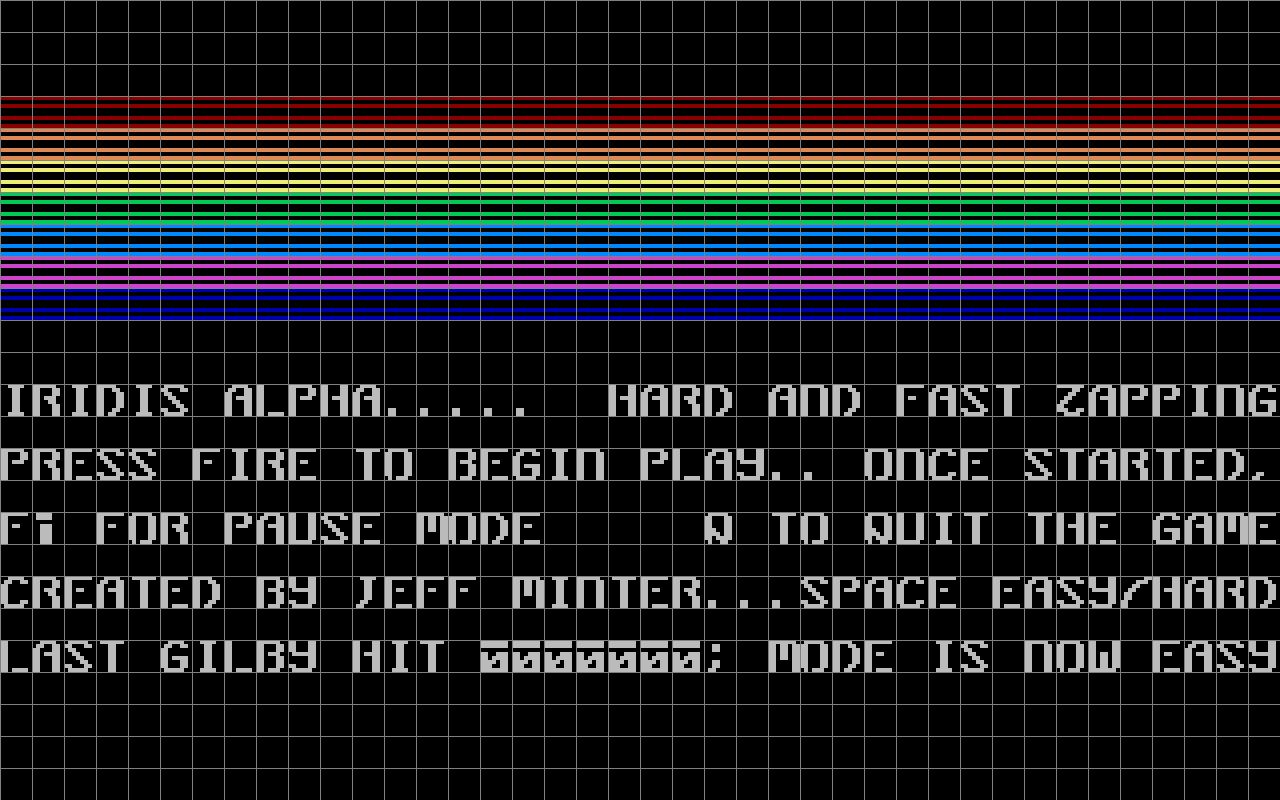
\includegraphics[width=13cm]{titlescreen/titlescreen_textonly_grid.png}%
    \end{adjustbox}
  \caption{The screen as it would appear after \icode{DrawStripesBehindTitle} and \icode{DrawTitleScreenText} have run. The added
  grid helps compare with our previous figures for \icode{SCREEN\_RAM} and \icode{COLOR\_RAM}.}
\end{figure}

\subsection{Racing the Beam}
Now we're ready to receive our ifirst beam. You may remember we set this to happen when the raster reached line 16:

\begin{lstlisting}[caption=In \icode{InitializeSpritesAndInterruptsForTitleScreen}]
        ; Set the position for triggering our interrupt.
        LDA #$10
        STA $D012    ;Raster Position
\end{lstlisting}

And that the routine we'll run when that happens is \icode{TitleScreenInterruptHandler} (which itself will pass
the work onto \icode{TitleScreenAnimation}:

\begin{lstlisting}[caption=In \icode{InitializeSpritesAndInterruptsForTitleScreen}]
        ; Set up the our interrupt handler for the title
        ; screen. This will do all the animation and title
        ; music work.
        LDA #<TitleScreenInterruptHandler
        STA $0314    ;IRQ
        LDA #>TitleScreenInterruptHandler
        STA $0315    ;IRQ
\end{lstlisting}

The painting of sprites and playing of music as the screen gets painted is all handled by \icode{TitleScreenAnimation}.
This routine works by calling one of three different sub-routines each time its called. It picks the one to run
depending on some internal state it maintains, all with a view to ensuring that the sprites spelling out the game's
title and the sprites depicting the animated gilbies are updated and in place before the raster reaches them.

To ensure it gets called by the interrupt when its needed it will repeatedly update the line that the next interrupt
should happen. We'll trace this as it actually happens, interrupt by interrupt, and sift through what the routine
does at each step during the raster's first pass at painting the entire screen.

The first time the raster is called, this is what the screen looks like:

\begin{figure}[H]
    \centering
      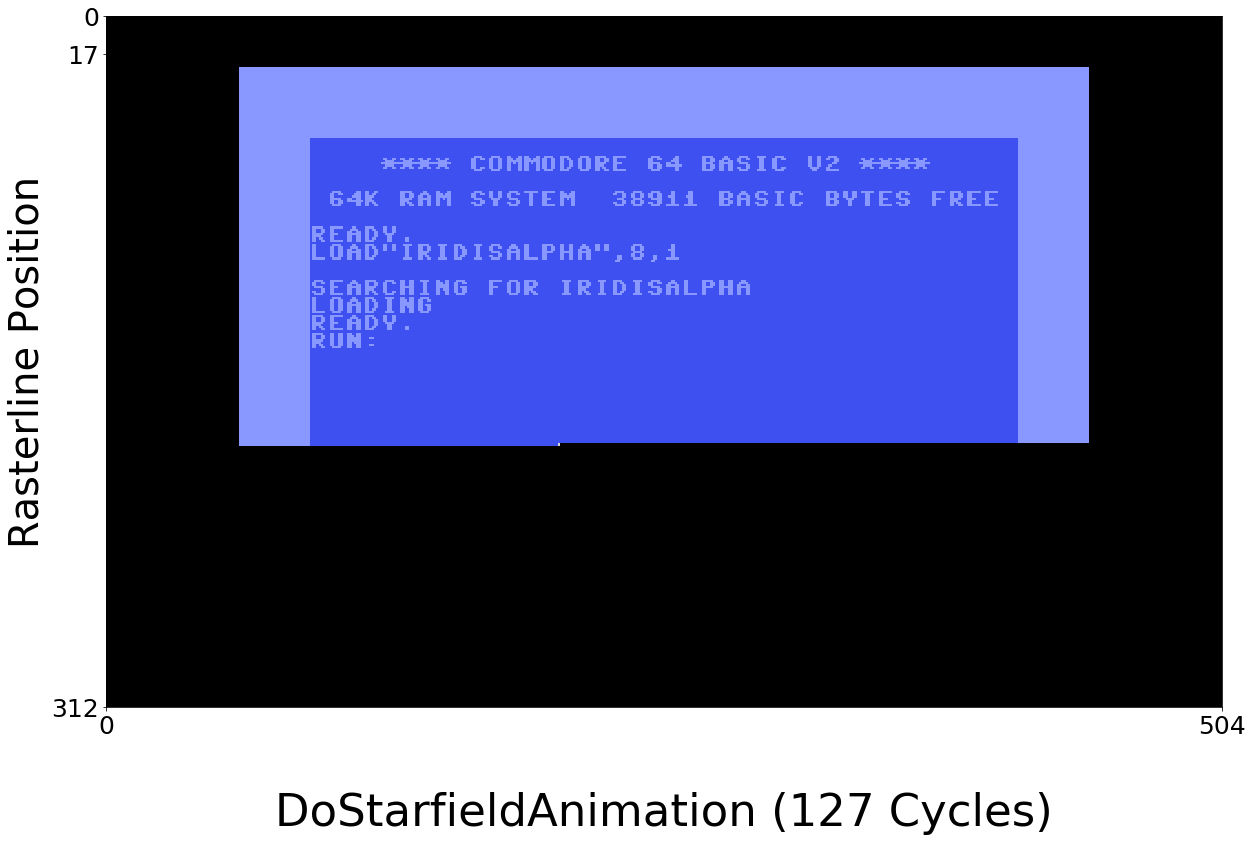
\includegraphics[width=10cm]{titlescreen/title1.png}%
\caption{The state of the screen the first time the raster interrupt is received at line 16.}
\end{figure}

Of course we never actually see the screen in this state because it only appears for a microsecond or two, much too
fast for us to observe. But as you can see the painting has aleady started. Everything above line 16 indicated in 
the figure has been painted black, as per our preparation of \icode{SCREEN\_RAM} a little earlier.

What our diagram above also tells us is that in this visit from the beam \icode{TitleScreenAnimation} chose to execute
the sub-routine \icode{DoStarfieldAnimation} and that it took 127 CPU cycles to complete it. Since it takes the
raster 63 cycles to do an entire line this means that by the time we've finished this piece of work, the raster will have
moved on to the next line - which is why the diagram shows 17 rather than 16. Every time we get an interrupt, the 
raster doesn't wait for us. We have to work quickly, especially if we're preparing graphics on lines that its likely
to reach soon. This is why each of these subroutines does as little as it can get away with to get the job done.

The three sub-routines the work at each raster interrupt can get divvied out to are \icode{UpdateJumpingGilbyPositionsAndColors},
\icode{DoStarfieldAnimation}, and a cluster of routines starting with \icode{UpdateTitleScreenSpriteColors}. The one
that's called the most often is \icode{DoStarfieldAnimation} as it is responsible for sprinkling the screen with 
animated stars traversing it left to right.

\begin{lstlisting}[caption=\icode{TitleScreenAnimation} responsible for choosing what to do at each interrupt. ]
;-------------------------------------------------------
; TitleScreenAnimation
; This handles all the activity in the title screen and is called
; roughly 60 times a second by the Raster Interrupt.
;-------------------------------------------------------
TitleScreenAnimation
        LDY titleScreenStarFieldAnimationCounter
        CPY #$0C
        BNE MaybeDoStarFieldOrTitleText

        JSR UpdateJumpingGilbyPositionsAndColors
        LDY #$10
        STY titleScreenStarFieldAnimationCounter

MaybeDoStarFieldOrTitleText   
        LDA titleScreenStarFieldYPosArray,Y
        BNE DoStarfieldAnimation

PaintTitleTextSprites
        JSR TitleScreenMutateStarfieldAnimationData

        LDA #$00
        STA titleScreenStarFieldAnimationCounter

        LDA #$10
        STA $D012    ;Raster Position

        ; Acknowledge the interrupt, so the CPU knows that
        ; we have handled it.
        LDA #$01
        STA $D019    ;VIC Interrupt Request Register (IRR)
        STA $D01A    ;VIC Interrupt Mask Register (IMR)

        JSR UpdateTitleTextSprites
        JSR MaybeUpdateSpriteColors
        JSR RecalculateJumpingGilbyPositions
        JSR PlayTitleScreenMusic
        JMP ReEnterInterrupt
        ; We're done, returns from function.
\end{lstlisting}

The internal accounting responsible for choosing the routine to run is tricky to decipher by just looking at the code. So
instead let's follow what actually happens in practice. If we roll ahead to the next interrupt we can already see something
happening:

\begin{figure}[H]
    \centering
      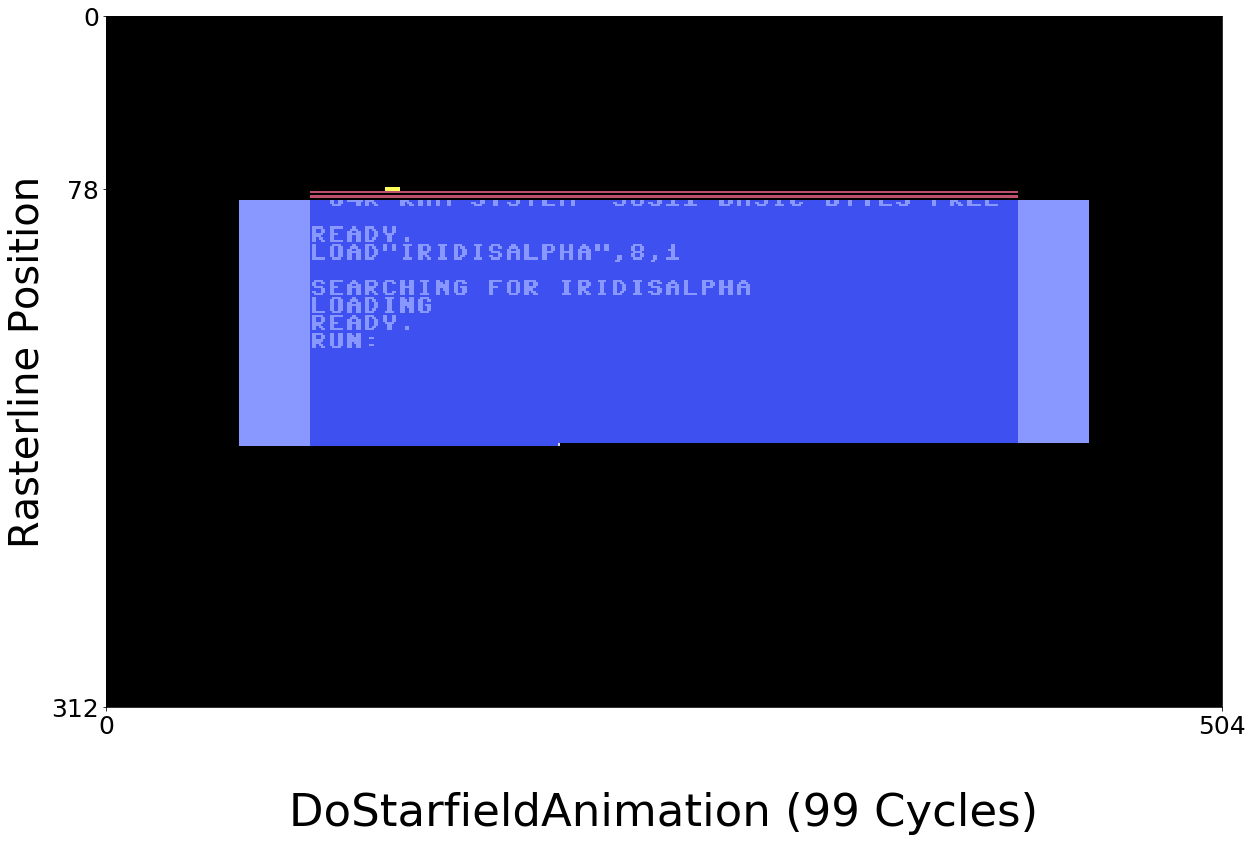
\includegraphics[width=10cm]{titlescreen/title3.png}%
\caption{The start of the stripes and a star.}
\end{figure}

If you look closely, you can see a yellow star painted over the first band of red stripes. This is our first sprite. You may
be wondering: what about the title sprites? Shouldn't they be there by now? The answer is no: we will paint them when the
raster reaches the end of the screen. When it goes to paint the screen a second time (the second 16 milliseconds) they
will be ready for painting. We'll see this in action a little later.

So let's see what \icode{DoStarfieldAnimation} did to get this sprite ready for painting.

When \icode{TitleScreenAnimation} chose \icode{DoStarfieldAnimation} as the sub-routine to run it loaded in a value
from \icode{titleScreenStarFieldYPosArray} to the \icode{A} register: 

\begin{lstlisting}
MaybeDoStarFieldOrTitleText   
        LDA titleScreenStarFieldYPosArray,Y
        BNE DoStarfieldAnimation
\end{lstlisting}

Since \icode{Y} is zero at this point this means it referenced the first value in the array, which is \icode{\$48}:
\begin{lstlisting}[basicstyle=\tiny]
titleScreenStarFieldYPosArray .BYTE $48,$4E,$54,$5A,$60,$66,$6C,$72
                              .BYTE $78,$7E,$84,$8A,$90,$96,$9C,$A2
                              .BYTE $A8,$AE,$B4,$BA,$C0,$C6,$CC,$D2
                              .BYTE $D8,$DE,$E4,$EA,$F0,$F6
titleScreenStarFieldXPosArray .BYTE $00,$3A,$1A,$C4,$1B,$94,$7B,$96
                              .BYTE $5D,$4F,$B5,$18,$C7,$E1,$EB,$4A
                              .BYTE $8F,$DA,$83,$6A,$B0,$FC,$68,$04
                              .BYTE $10,$06,$A7,$B8,$19,$BB
\end{lstlisting}

So when \icode{DoStarfieldAnimation} is called the first thing it does is set the y position of the star to paint
to \icode{\$48} (72 in decimal): 

\begin{lstlisting}[caption=The start of \icode{DoStarfieldAnimation} responsible for painting stars.]
DoStarfieldAnimation   
        ; A was loaded from titleScreenStarFieldYPosArray
        ; by the caller.
        STA $D00F    ;Sprite 7 Y Pos

        ; Set the X position of the star.
        LDA titleScreenStarFieldXPosArray + $01,Y
        STA $D00E    ;Sprite 7 X Pos

\end{lstlisting}

You can also see it then sets the X position of the star using values plucked from \icode{titleScreenStarFieldXPosArray}.
So we're leaning heavily on these two arrays to decide where to place stars. But so far, so simple. We've placed the star
on the screen more or less and when the raster reaches line 72 it will paint it. There's an additional complication to 
specifying the X coordinate of the star though and we can't really gloss over it here. We'll also encounter this
wrinkle elsewhere too so it's worth pausing on for a moment.

The next few lines of the routine do quite a bit of convoluted work to handle something called the \icode{spriteMSBXPosOffset} of the
star. This is our complication. 

\subsubsection{A Complication}
\begin{lstlisting}[caption= MSBXPos.. some'it.]
        ; Set the rest of the X position of the star
        ; if it's greater than 255.
        LDA titleScreenStarfieldMSBXPosArray + $01,Y
        AND #$01
        STA spriteMSBXPosOffset

        BEQ StarFieldSkipMSB

        LDA #$80
        STA spriteMSBXPosOffset
StarFieldSkipMSB   
        LDA $D010    ;Sprites 0-7 MSB of X coordinate
        AND #$7F
        ORA spriteMSBXPosOffset
        STA $D010    ;Sprites 0-7 MSB of X coordinate

\end{lstlisting}

If you look at the diagram again you may recall we said the screen we're painting is 504 pixels wide. Fortunately the only 
part we can paint is the section in the center that is 320 pixels wide and 200 pixels high. 

\begin{figure}[H]
    \centering
      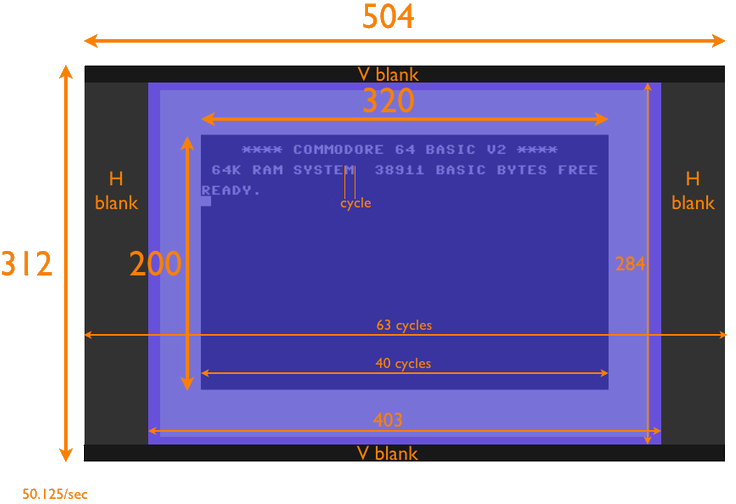
\includegraphics[width=10cm]{titlescreen/raster.png}%
  \caption{The different parts of the screen, we can only paint the bit in the middle. (Source: dustlayer.com)}
\end{figure}

200 is a value that can be expressed with a single byte. However, 320 is not. A byte can only store a number up to 255
so if we want to specify an X co-ordinate greater than 255 a single byte will not do. The way the C64 works around this
is by making a single extra bit for our sprite's X co-ordinate available that brings the available values up from 256
(0 - 255) to 512. Since there are 8 sprites in total we need 8 extra bits to cover this requirement for all of them.
For this purpose we use a single byte at address \icode{\$D010} that contains the extra bit for all 8 sprites. We refer
to this bit as the \icode{MSB} for the X co-ordinate because it is the 'Most Significant Bit', i.e. the left most bit,
in the 9-bit number that we store the X co-ordinate in. That's to say our x co-ordinate is given by combining the value
between 0 and 255 we store in our 8-bit byte for 'Sprite 7' in \icode{\$D00E} and the extra bit we store in \icode{\$D010}.

\begin{figure}[H]
  {
    \setlength{\tabcolsep}{3.0pt}
    \setlength\cmidrulewidth{\heavyrulewidth} % Make cmidrule = 
    \begin{adjustbox}{width=10cm,center}

      \begin{tabular}{rllllllll}
        \toprule
        Sprite 7 & Sprite 6 & Sprite 5 & Sprite 4 & Sprite 3 & Sprite 2 & Sprite 1 & Sprite 0        \\
        \midrule
        Bit 7 & Bit 6 & Bit 5 & Bit 4 & Bit 3 & Bit 2 & Bit 1 & Bit 0        \\
        \midrule
        0 & 0 & 0 & 0 & 0 & 0 & 0 & 0 \\
        \addlinespace
        \bottomrule
      \end{tabular}

    \end{adjustbox}

  }\caption*{The most significant bits in \icode{\$D010} for each sprite.}
\end{figure}

Since we are using 'Sprite 7' for painting the starfield the bit we are interested in is bit 7. The way
we're going to manage this value for the starfield is by keeping array \icode{titleScreenStarfieldMSBXPosArray}
that indicates whether the x co-ordinate for the current index is greater than 255. If the value in there
indicates that it is we'll set our bit in \icode{\$D010} to 1.

So when
we determine from looking in \icode{titleScreenStarfieldMSBXPosArray} that the x co-ordinate of the star is greater
than 256..

\begin{lstlisting}[basicstyle=\tiny]
        LDA titleScreenStarfieldMSBXPosArray + $01,Y
        AND #$01
        STA spriteMSBXPosOffset
\end{lstlisting}

.. we set \icode{spriteMSBXPosOffset} to indicate that that's the case. That's all this step, with the help
of the \icode{AND \#\$01} statement is doing. If 'Bit 1' is
set in the value we pluck from \icode{titleScreenStarfieldMSBXPosArray} it is just an indicator that the x co-ordinate
for this star is greater than 256. So if we see a value of \icode{\$02} in there our operation \icode{AND \#\$01} will
give us a zero result, meaning the intended value of the x co-ordinate is not greater than 256, othwerise it will give
us a non-zero result indicating that it is:

\begin{figure}[H]
  {
    \setlength{\tabcolsep}{3.0pt}
    \setlength\cmidrulewidth{\heavyrulewidth} % Make cmidrule = 
    \begin{adjustbox}{width=10cm,center}

      \begin{tabular}{rllllllll}
        \toprule
        Byte & Bit 7 & Bit 6 & Bit 5 & Bit 4 & Bit 3 & Bit 2 & Bit 1 & Bit 0        \\
        \midrule
        \$02 & 0 & 0 & 0 & 0 & 0 & 0 & 1 & 0 \\
        \$01 & 0 & 0 & 0 & 0 & 0 & 0 & 0 & 1 \\
        \midrule
        Result: \$00 & 0 & 0 & 0 & 0 & 0 & 0 & 0 & 0 \\
        \addlinespace
        \bottomrule
      \end{tabular}
    \end{adjustbox}
  }\caption*{AND'ing \$02 and \$01 gives \$00 (0). For \icode{AND} to give a 1 both bits must 1 or both must be 0.}
\end{figure}

This zero result allows \icode{BEQ StarFieldSkipMSB} to evaluate as \icode{True} so we skip ahead to \icode{StarFieldSkipMSB}
to set \icode{\$D010}.
It means for us that the value of the x co-ordinate is not going to be greater than 255. If this is not the case, we instead load a value of
\icode{\$80} to \icode{spriteMSBXPosOffset} to overwrite the \icode{00} there. This will indicate that the value of the x co-ordinate
is greater than 255.

\begin{lstlisting}[basicstyle=\tiny]
        BEQ StarFieldSkipMSB

        LDA #$80
        STA spriteMSBXPosOffset
StarFieldSkipMSB   
        LDA $D010    ;Sprites 0-7 MSB of X coordinate
        AND #$7F
        ORA spriteMSBXPosOffset
        STA $D010    ;Sprites 0-7 MSB of X coordinate
\end{lstlisting}

The remaining step above is to load the value we've arrived at in \icode{spriteMSBXPosOffset} to \icode{\$D010}. Since we
want to do this without affecting any of the other bits in there that have been set for the other sprites we can't
just do a \icode{LDA/STA} as that will overwrite what's already there. The combination of the \icode{AND/OR} operations
here accomplishes something quite nifty - it allows us to update just the bit (Bit 7) that interests us in \icode{\$D010}.

If we suppose the current value in \icode{\$D010} is \icode{\$F3}, our \icode{AND \#\$7F} operation clears 'Bit 7' so that
it is always set to zero:

\begin{figure}[H]
  {
    \setlength{\tabcolsep}{3.0pt}
    \setlength\cmidrulewidth{\heavyrulewidth} % Make cmidrule = 
    \begin{adjustbox}{width=10cm,center}

      \begin{tabular}{rllllllll}
        \toprule
        Byte & Bit 7 & Bit 6 & Bit 5 & Bit 4 & Bit 3 & Bit 2 & Bit 1 & Bit 0        \\
        \midrule
        \$F3 & 1 & 1 & 1 & 1 & 0 & 0 & 1 & 1 \\
        \$7F & 0 & 1 & 1 & 1 & 1 & 1 & 1 & 1 \\
        \midrule
        Result: \$73 & 0 & 1 & 1 & 1 & 0 & 0 & 1 & 1 \\
        \addlinespace
        \bottomrule
      \end{tabular}
    \end{adjustbox}
  }\caption*{AND'ing \$F3 and \$00 gives \$73. It clears 'Bit 7' for us of whatever value was there originally.}
\end{figure}

Now when we perform an 'or' operation on the result with \icode{ORA spriteMSBXPosOffset} it will have the effect of just setting 'Bit 7'
with the value we've stored in \icode{spriteMSBXPosOffset}. In this case it remains at zero because that's what we have in
\icode{spriteMSBXPosOffset} but if we have \icode{\$80} in there it would set it to 1: 

\begin{figure}[H]
  {
    \setlength{\tabcolsep}{3.0pt}
    \setlength\cmidrulewidth{\heavyrulewidth} % Make cmidrule = 
    \begin{adjustbox}{width=10cm,center}

      \begin{tabular}{rllllllll}
        \toprule
        Byte & Bit 7 & Bit 6 & Bit 5 & Bit 4 & Bit 3 & Bit 2 & Bit 1 & Bit 0        \\
        \midrule
        \$73 & 0 & 1 & 1 & 1 & 0 & 0 & 1 & 1 \\
        \$00 & 0 & 0 & 0 & 0 & 0 & 0 & 0 & 0 \\
        \midrule
        Result: \$73 & 0 & 1 & 1 & 1 & 0 & 0 & 1 & 1 \\
        \addlinespace
        \bottomrule
      \end{tabular}
    \end{adjustbox}
  }\caption*{OR'ing \$73 and \$00 gives \$73.}
\end{figure}

\subsubsection{Back to the Beam}
Now that we've fixed the star's co-ordinates there's just two main things left to do before we're done with
handling this raster interrupt. One is to set the color of the star. We do this using a look-up array
where we get the color for the star per our current index and set it:

\begin{lstlisting}
        LDA titleScreenStarFieldColorsArrayLookUp,Y
        TAX
        LDA titleScreenColorsArray - $01,X
        STA $D02E    ;Sprite 7 Color
\end{lstlisting}

The second, and most important, is that we update the position on the screen that we want the next interrupt to
happen. Remember for this visit we were interrupted at line 17. We want to place stars on other lines so we keep
a list of the lines we want to write stars on in \icode{titleScreenStarFieldYPosArray}, i.e. an array that
stores the y co-ordinates of our stars. What we do is simply update the Raster Interrupt with the next position
from this array so that we get called when the raster reaches it:

\begin{lstlisting}
        ; Update the raster position for the next interrupt
        ; to the current line - 1. This will allow us to 
        ; draw the sprite multiple times on different lines.
        LDA titleScreenStarFieldYPosArray + $01,Y
        SEC
        SBC #$01
        STA $D012    ;Raster Position
\end{lstlisting}

In this instance we're setting the value to \icode{\$48} (72). So when the next interrupt happens it will reveal
the star we just prepared. THis is the one we took a peek at in Figure 1.10.

The next ten interrupts will continue to revisit \icode{DoStarfieldAnimation}. Let's look at the screen
as it unfolds through each of these interrupts:

\begin{figure}[H]
    \centering
    \foreach \l in {5, 7, ...,23}
    {
      \includegraphics[width=4cm]{titlescreen/title\l.png}%
    }%
\caption{The next ten interrupts paint the starfield on the screen until we reach the point at which we want to prepare
  the gilby sprites.}
\end{figure}

\subsection{Enter The Gilbies}
\begin{figure}[H]
    \centering
      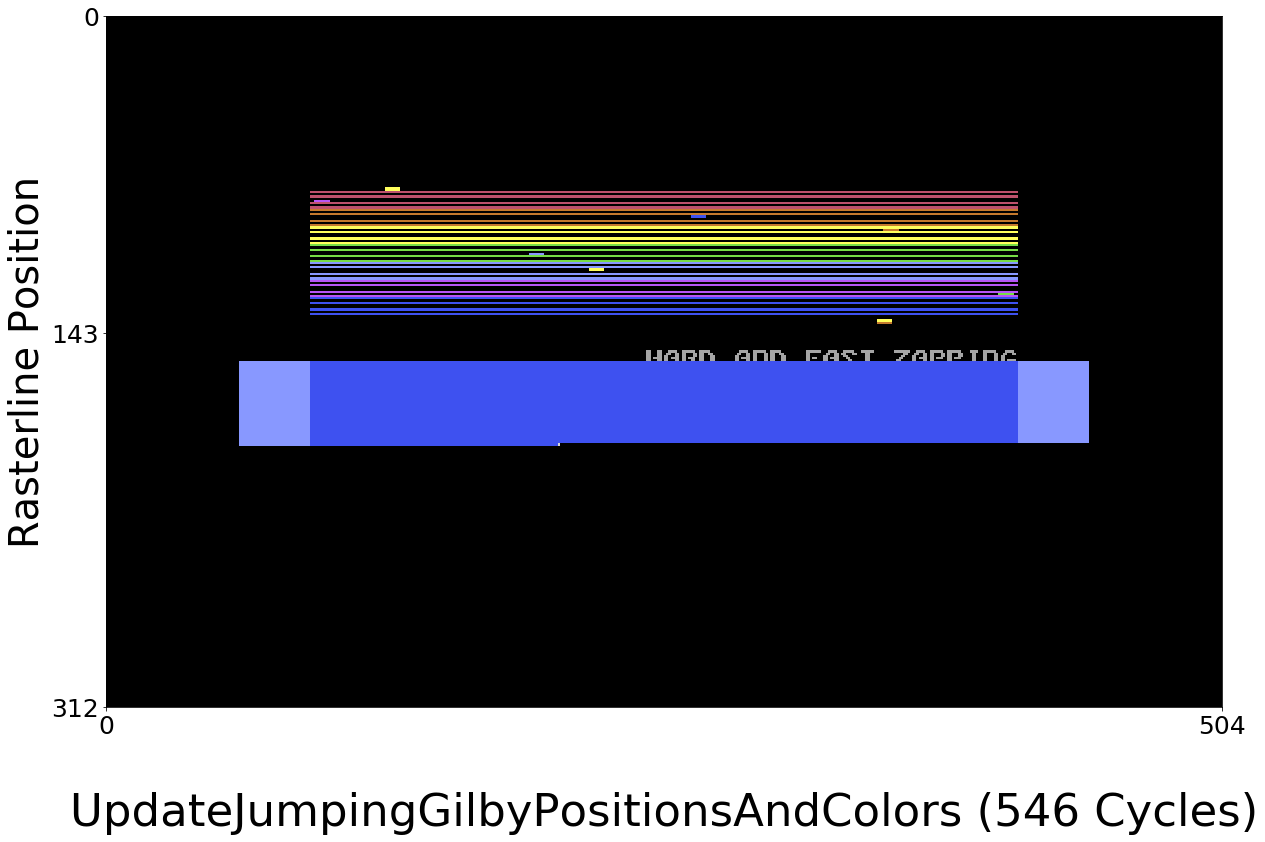
\includegraphics[width=12cm]{titlescreen/title25.png}%
\caption{The point we reach in the screen paint when we decide to prepare the gilby sprites.}
\end{figure}

Finally we've reached a point in the screen where we're not just going to add another star to the background.
We've been keeping a count of the number of interrupts we've handled in \icode{titleScreenStarFieldAnimationCounter}.
When it reaches \icode{\$0C} (12) we've handled the raster interrupt twelve times and painted nothing but the
text background we prepared earlier and the stars we've added along the way. Now's the time to do something else:

\begin{lstlisting}
TitleScreenAnimation
        LDY titleScreenStarFieldAnimationCounter
        CPY #$0C
        BNE MaybeDoStarFieldOrTitleText

        JSR UpdateJumpingGilbyPositionsAndColors
        LDY #$10
        STY titleScreenStarFieldAnimationCounter
\end{lstlisting}

The routine we call into here by the name of \icode{UpdateJumpingGilbyPositionsAndColors} will prepare the sequence
of jumping rainbow gilbies somewhere in the lower half of the screen before our current raster line. That's why we
call it at this point in the raster's journey - because the raster hasn't reached that position in the screen yet
(but will reach it shortly) so now is our opportunity to position the gilbies where we want them. 

Since this is an animation sequence we're managing the approach of \icode{UpdateJumpingGilbyPositionsAndColors} is
simply to update their position on the screen. Calculating this new position is something that happens a little later
in the routine \icode{RecalculateJumpingGilbyPositions} when we are nearer the bottom of the screen. This means the
position values we're picking up here are the initial ones set in the game's code:

\begin{lstlisting}
titleScreenGilbiesYPosArray       .BYTE $B2,$B6,$BB,$C1,$D0,$C8,$C1
titleScreenGilbiesXPosArray       .BYTE $54,$58,$5C,$60,$64,$68,$6C
\end{lstlisting}

The next time around we will pick up the positions as re-calculated by \icode{RecalculateJumpingGilbyPositions}.
So the positioning of the gilbies and the calculation of the updated positions happen separately. The reason
for that approach is simple: there isn't enough time right now to do anything but simply update the positions the gilbies
are displayed at.
Later on, when the raster has passed line 320 we will have a lot more time available to perform complex calculations
because we don't need to worry about the raster painting anything on the screen for a while.

Since there are 7 of them, setting the x and y co-ordinates of the seven gilby sprites is handled by a loop:

\begin{lstlisting}[caption= The loop in \icode{UpdateJumpingGilbyPositionsAndColors} updating the x and y position on screen and color of each of the gilby sprites.]
        ; Loop through the gilby sprites in the title screen and
        ; update their position and color
        LDX #$00
UpdateJumpingGilbiesLoop   
        TXA
        ASL
        TAY
        LDA titleScreenGilbiesXPosArray,X
        ASL
        STA $D000,Y  ;Sprite 0 X Pos
        BCC SkipGilbyMSBXPos
        LDA $D010    ;Sprites 0-7 MSB of X coordinate
        ORA titleScreenGilbiesMSBXPosArray,X
        STA $D010    ;Sprites 0-7 MSB of X coordinate
        JMP UpdateYPosJumpingGilbies

SkipGilbyMSBXPos   
        LDA $D010    ;Sprites 0-7 MSB of X coordinate
        AND titleScreenGilbiesMSBXPosOffset,X
        STA $D010    ;Sprites 0-7 MSB of X coordinate

UpdateYPosJumpingGilbies
        LDA titleScreenGilbiesYPosARray,X
        STA $D001,Y  ;Sprite 0 Y Pos

        LDA currentTitleScreenGilbySpriteValue
        STA Sprite0Ptr,X

        ; Update Gilby color.
        LDA titleScreenColorsArray,X
        STA $D027,X  ;Sprite 0 Color

        INX
        CPX #$07
        BNE UpdateJumpingGilbiesLoop
        RTS
\end{lstlisting}
We can see in here the verbosity required to handle the most significant bit of the sprite's x co-ordinate. Just
as with the starfield we need a separate array (\icode{titleScreenGilbiesMSBXPosArray} to handle this in addition
to arrays to manage the basic x/y positions themselves.

With the gilbies prepared we fall through and update the starfield again. Once that's done we're finished handling the
current raster interrupt. This is followed by another dozen or so interrupts where we again just prepare stars for display
and as the raster progress our gilbies are revealed.

\begin{figure}[H]
    \centering
    \foreach \l in {27, 29, ..., 55}
    {
      \begin{subfigure}{0.3\textwidth}
      \includegraphics[width=4cm]{titlescreen/title\l.png}%
      \end{subfigure}
    }%
\caption{Behold the gilbies.}
\end{figure}

\subsection{Title Text}
\begin{figure}[H]
    \centering
      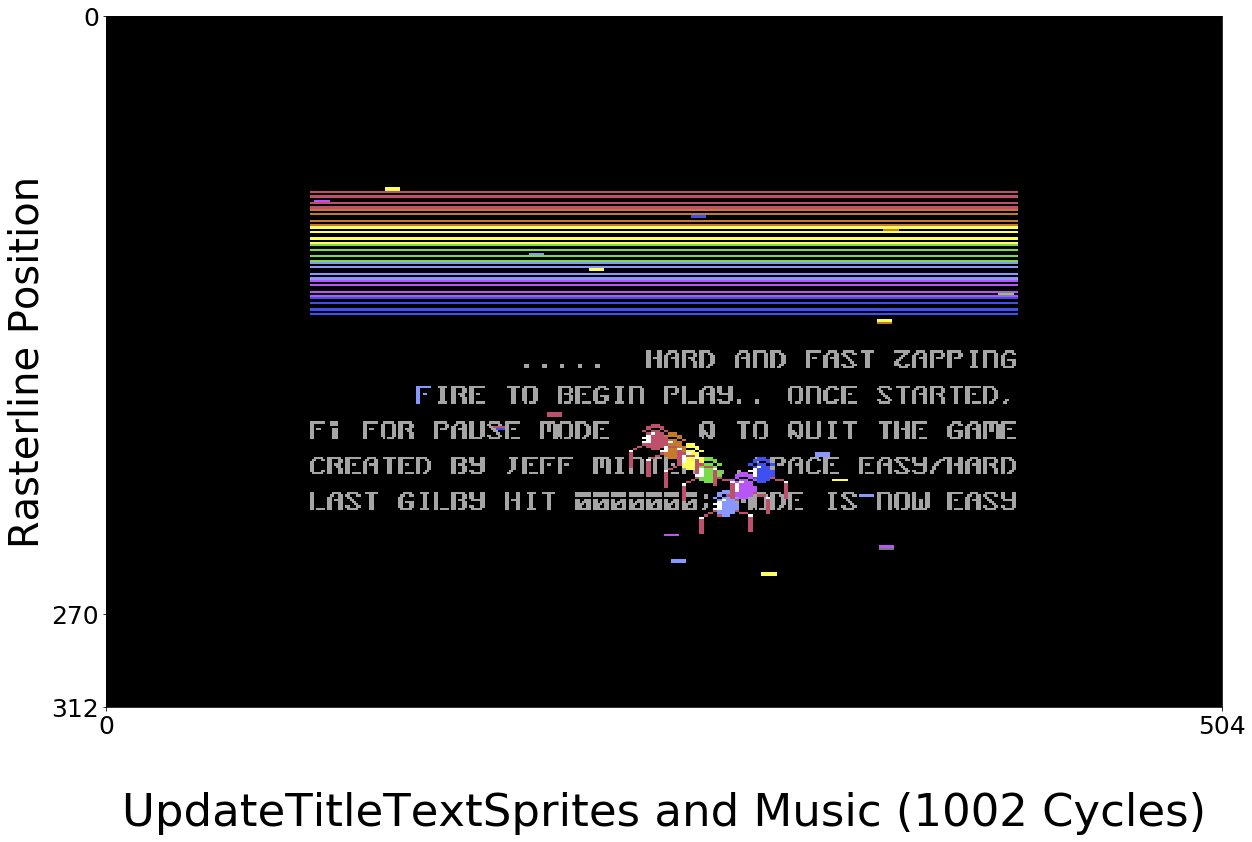
\includegraphics[width=12cm]{titlescreen/title57.png}%
\caption{We've finally reached the bottom of the screen, with gilbies and stars painted, but still no title.}
\end{figure}

We've finally reached the bottom of the screen in our first raster paint, at least the bottom of the portion of the
screen that we can paint. When the raster hits line 270 we're beyond the point that we can place anything on the screen and
into the border area. This gives us time to do some more complicated and time consuming stuff.

There's a relatively full agenda:

\begin{lstlisting}
        LDA #$10
        STA $D012    ;Raster Position

        ; Acknowledge the interrupt, so the CPU knows that
        ; we have handled it.
        LDA #$01
        STA $D019    ;VIC Interrupt Request Register (IRR)
        STA $D01A    ;VIC Interrupt Mask Register (IMR)

        ; All of this stuff can be done before the raster
        ; reaches the top of the screen again.
        JSR UpdateTitleTextSprites
        JSR MaybeUpdateSpriteColors
        JSR RecalculateJumpingGilbyPositions
        JSR PlayTitleScreenMusic
        JMP ReEnterInterrupt
\end{lstlisting}

First of all we set the raster interrupt to line 16 at the top of the screen again, then we acknowledge the interrupt. The
raster will continue its journey but because we're going to do this while it works its way the next 42 lines at the bottom 
of the screen we have more time than at any point previously to get things done.

Adding the title sprites is relatively light work. Just as with the gilbies we use a tight loop to paint each of them
on the screen. THere's no animation to handle here.

\begin{lstlisting}
titleTextSpriteArray          .BYTE $20,BIG_I,BIG_R,BIG_I,BIG_D,BIG_I,BIG_S
...

PaintSpriteLettersLoop   
        ; Assign the sprite.
        LDA titleTextSpriteArray,X
        STA Sprite0Ptr - $01,X

        ; Shift the value in X left 1 bit and assign to Y.
        ; So e.g. 6 becomes 12, 5 becomes 10, 4 becomes 8,
        ; 3 becomes 6 and so on. This allows us to use Y
        ; as an offset to the appropriate item in $D000-
        ; $D012 for updating the sprite's position.
        TXA
        ASL
        TAY

        ; Update the X Position of the sprite
        LDA titleTextXPosArray - $01,X
        STA $D000 - $02,Y

        LDA $D010    ;Sprites 0-7 MSB of X coordinate
        ORA titleTextMSBXPosArray,X
        STA $D010    ;Sprites 0-7 MSB of X coordinate

        ; Update the Y position of the sprite
        LDA #$40
        STA $D000 - $01,Y
        DEX
        BNE PaintSpriteLettersLoop

\end{lstlisting}

The other complex thing we do is calculate the next step in the jumping gilby animations. \icode{RecalculateJumpingGilbyPositions}
updates the x and y positions of the gilby sprites in \icode{titleScreenGilbiesYPosArray} and \icode{titleScreenGilbiesXPosArray}.

Finally we play a single note from the title music, we cover this in detail in a later chapter.

The raster continues on its journey and progresses through its second paint journey of the screen. The title sprites
are finally revealed.

\begin{figure}[H]
    \centering
    \foreach \l in {59, 61, ..., 81}
    {
      \begin{subfigure}{0.3\textwidth}
      \includegraphics[width=4cm]{titlescreen/title\l.png}%
      \end{subfigure}
    }%
\caption{The title text is finally revealed}
\end{figure}

And with that the title sequence is finally up and running after 20 milliseconds or so.

\begin{figure}[H]
    \centering
      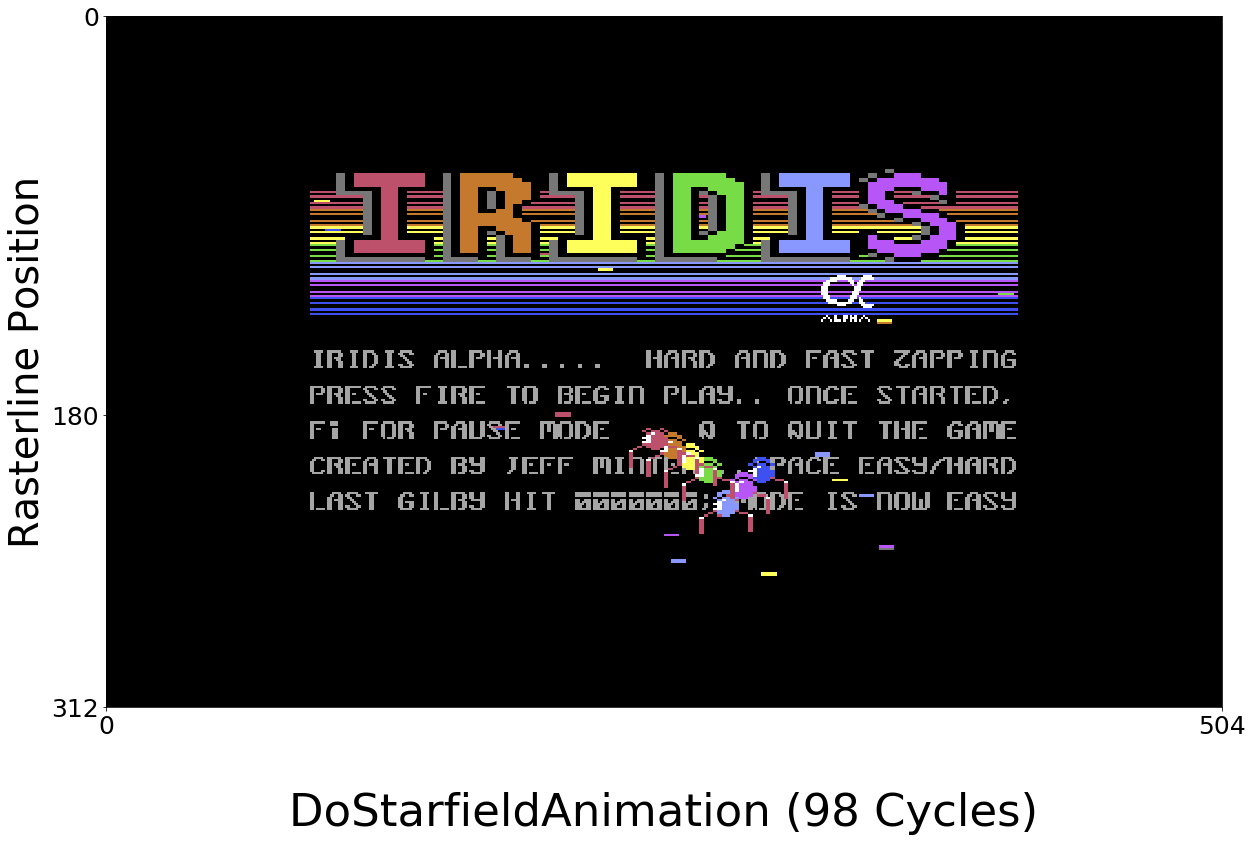
\includegraphics[width=12cm]{titlescreen/title89.png}%
\caption{We're done here.}
\end{figure}
